% =====================================================================
% HOL Manual LaTeX Source: tutorial
% =====================================================================

\documentclass[12pt,fleqn]{book}
%\usepackage{amsmath}
\usepackage{alltt}
\usepackage{../LaTeX/layout}
\usepackage{graphicx}
%HEVEA \usepackage{epsfig}
%PVH \usepackage{verbatim}

\renewcommand\leadsto\rightarrow

% ---------------------------------------------------------------------
% Input defined macros and commands
% ---------------------------------------------------------------------
% =====================================================================
%
% Macros for typesetting the HOL system manual
%
% =====================================================================

% ---------------------------------------------------------------------
% Abbreviations for words and phrases
% ---------------------------------------------------------------------

\newcommand\TUTORIAL{{\footnotesize\sl TUTORIAL}}
\newcommand\DESCRIPTION{{\footnotesize\sl DESCRIPTION}}
\newcommand\REFERENCE{{\footnotesize\sl REFERENCE}}
\newcommand\LOGIC{{\footnotesize\sl LOGIC}}
\newcommand\LIBRARIES{{\footnotesize\sl LIBRARIES}}

\newcommand{\bs}{\texttt{\char'134}} % backslash
\newcommand{\lb}{\texttt{\char'173}} % left brace
\newcommand{\rb}{\texttt{\char'175}} % right brace
\newcommand{\td}{\texttt{\char'176}} % tilde
\newcommand{\lt}{\texttt{\char'74}} % less than
\newcommand{\gt}{\texttt{\char'76}} % greater than
\newcommand{\dol}{\texttt{\char'44}} % dollar
% double back quotes ``
\newcommand{\dq}{\texttt{\char'140\char'140}}
%These macros were included by slind:

\newcommand{\holquote}[1]{\dq#1\dq}

\def\HOL{{\small HOL}}
\def\holn{\HOL}  % i.e. hol n(inety-eight), no digits in
                 % macro names is a bit of a pain; deciding to do away
                 % with hol98 nomenclature means that we just want to
                 % write HOL for hol98.
\def\holnversion{Kananaskis-7}
\def\holnsversion{Kananaskis~7} % version with space rather than hyphen
\def\LCF{{\small LCF}}
\def\LCFLSM{{\small LCF{\kern-.2em}{\normalsize\_}{\kern0.1em}LSM}}
\def\PPL{{\small PP}{\kern-.095em}$\lambda$}
\def\PPLAMBDA{{\small PPLAMBDA}}
\def\ML{{\small ML}}
\def\holmake{\texttt{Holmake}}

\newcommand\ie{\mbox{i{.}e{.}}}
\newcommand\eg{\mbox{e{.}g{.}}}
\newcommand\viz{\mbox{viz{.}}}
\newcommand\adhoc{\mbox{\it ad hoc}}
\newcommand\etal{{\it et al.\/}}
\newcommand\etc{\mbox{etc{.}}}

% ---------------------------------------------------------------------
% Simple abbreviations and macros for mathematical typesetting
% ---------------------------------------------------------------------

\newcommand\fun{{\to}}
\newcommand\prd{{\times}}

\newcommand\conj{\ \wedge\ }
\newcommand\disj{\ \vee\ }
\newcommand\imp{ \Rightarrow }
\newcommand\eqv{\ \equiv\ }
\newcommand\cond{\rightarrow}
\newcommand\vbar{\mid}
\newcommand\turn{\ \vdash\ }
\newcommand\hilbert{\varepsilon}
\newcommand\eqdef{\ \equiv\ }

\newcommand\natnums{\mbox{${\sf N}\!\!\!\!{\sf N}$}}
\newcommand\bools{\mbox{${\sf T}\!\!\!\!{\sf T}$}}

\newcommand\p{$\prime$}
\newcommand\f{$\forall$\ }
\newcommand\e{$\exists$\ }

\newcommand\orr{$\vee$\ }
\newcommand\negg{$\neg$\ }

\newcommand\arrr{$\rightarrow$}
\newcommand\hex{$\sharp $}

\newcommand{\uquant}[1]{\forall #1.\ }
\newcommand{\equant}[1]{\exists #1.\ }
\newcommand{\hquant}[1]{\hilbert #1.\ }
\newcommand{\iquant}[1]{\exists ! #1.\ }
\newcommand{\lquant}[1]{\lambda #1.\ }

\newcommand{\leave}[1]{\\[#1]\noindent}
\newcommand\entails{\mbox{\rule{.3mm}{4mm}\rule[2mm]{.2in}{.3mm}}}

% ---------------------------------------------------------------------
% Font-changing commands
% ---------------------------------------------------------------------

\newcommand{\theory}[1]{\hbox{{\small\tt #1}}}
\newcommand{\theoryimp}[1]{\texttt{#1}}

\newcommand{\con}[1]{{\sf #1}}
\newcommand{\rul}[1]{{\tt #1}}
\newcommand{\ty}[1]{\textsl{#1}}

\newcommand{\ml}[1]{\mbox{{\def\_{\char'137}\texttt{#1}}}}
\newcommand{\holtxt}[1]{\ml{#1}}
\newcommand\ms{\tt}
\newcommand{\s}[1]{{\small #1}}

\newcommand{\pin}[1]{{\bf #1}}
\def\m#1{\mbox{\normalsize$#1$}}

% ---------------------------------------------------------------------
% Abbreviations for particular mathematical constants etc.
% ---------------------------------------------------------------------

\newcommand\T{\con{T}}
\newcommand\F{\con{F}}
\newcommand\OneOne{\con{One\_One}}
\newcommand\OntoSubset{\con{Onto\_Subset}}
\newcommand\Onto{\con{Onto}}
\newcommand\TyDef{\con{Type\_Definition}}
\newcommand\Inv{\con{Inv}}
\newcommand\com{\con{o}}
\newcommand\Id{\con{I}}
\newcommand\MkPair{\con{Mk\_Pair}}
\newcommand\IsPair{\con{Is\_Pair}}
\newcommand\Fst{\con{Fst}}
\newcommand\Snd{\con{Snd}}
\newcommand\Suc{\con{Suc}}
\newcommand\Nil{\con{Nil}}
\newcommand\Cons{\con{Cons}}
\newcommand\Hd{\con{Hd}}
\newcommand\Tl{\con{Tl}}
\newcommand\Null{\con{Null}}
\newcommand\ListPrimRec{\con{List\_Prim\_Rec}}


\newcommand\SimpRec{\con{Simp\_Rec}}
\newcommand\SimpRecRel{\con{Simp\_Rec\_Rel}}
\newcommand\SimpRecFun{\con{Simp\_Rec\_Fun}}
\newcommand\PrimRec{\con{Prim\_Rec}}
\newcommand\PrimRecRel{\con{Prim\_Rec\_Rel}}
\newcommand\PrimRecFun{\con{Prim\_Rec\_Fun}}

\newcommand\bool{\ty{bool}}
\newcommand\num{\ty{num}}
\newcommand\ind{\ty{ind}}
\newcommand\lst{\ty{list}}

% ---------------------------------------------------------------------
% \minipagewidth = \textwidth minus 1.02 em
% ---------------------------------------------------------------------

\newlength{\minipagewidth}
\setlength{\minipagewidth}{\textwidth}
\addtolength{\minipagewidth}{-1.02em}

% ---------------------------------------------------------------------
% Environment for the items on the title page of a case study
% ---------------------------------------------------------------------

\newenvironment{inset}[1]{\noindent{\large\bf #1}\begin{list}%
{}{\setlength{\leftmargin}{\parindent}%
\setlength{\topsep}{-.1in}}\item }{\end{list}\vskip .4in}

% ---------------------------------------------------------------------
% Macros for little HOL sessions displayed in boxes.
%
% Usage: (1) \setcounter{sessioncount}{1} resets the session counter
%
%        (2) \begin{session}\begin{verbatim}
%             .
%              < lines from hol session >
%             .
%            \end{verbatim}\end{session}
%
%            typesets the session in a numbered box.
% ---------------------------------------------------------------------

\newlength{\hsbw}
\setlength{\hsbw}{\textwidth}
\addtolength{\hsbw}{-\arrayrulewidth}
\addtolength{\hsbw}{-\tabcolsep}
\newcommand\HOLSpacing{13pt}

\newcounter{sessioncount}
\setcounter{sessioncount}{0}

\newenvironment{session}{\begin{flushleft}
 \refstepcounter{sessioncount}
 \begin{tabular}{@{}|c@{}|@{}}\hline
 \begin{minipage}[b]{\hsbw}
 \vspace*{-.5pt}
 \begin{flushright}
 \rule{0.01in}{.15in}\rule{0.3in}{0.01in}\hspace{-0.35in}
 \raisebox{0.04in}{\makebox[0.3in][c]{\footnotesize\sl \thesessioncount}}
 \end{flushright}
 \vspace*{-.55in}
 \begingroup\small\baselineskip\HOLSpacing}{\endgroup\end{minipage}\\ \hline
 \end{tabular}
 \end{flushleft}}

% ---------------------------------------------------------------------
% Macro for boxed ML functions, etc.
%
% Usage: (1) \begin{holboxed}\begin{verbatim}
%               .
%               < lines giving names and types of mk functions >
%               .
%            \end{verbatim}\end{holboxed}
%
%            typesets the given lines in a box.
%
%            Conventions: lines are left-aligned under the "g" of begin,
%            and used to highlight primary reference for the ml function(s)
%            that appear in the box.
% ---------------------------------------------------------------------

\newenvironment{holboxed}{\begin{flushleft}
  \begin{tabular}{@{}|c@{}|@{}}\hline
  \begin{minipage}[b]{\hsbw}
% \vspace*{-.55in}
  \vspace*{.06in}
  \begingroup\small\baselineskip\HOLSpacing}{\endgroup\end{minipage}\\ \hline
  \end{tabular}
  \end{flushleft}}

% ---------------------------------------------------------------------
% Macro for unboxed ML functions, etc.
%
% Usage: (1) \begin{hol}\begin{verbatim}
%               .
%               < lines giving names and types of mk functions >
%               .
%            \end{verbatim}\end{hol}
%
%            typesets the given lines exactly like {boxed}, except there's
%            no box.
%
%            Conventions: lines are left-aligned under the "g" of begin,
%            and used to display ML code in verbatim, left aligned.
% ---------------------------------------------------------------------

\newenvironment{hol}{\begin{flushleft}
 \begin{tabular}{c@{}@{}}
 \begin{minipage}[b]{\hsbw}
% \vspace*{-.55in}
 \vspace*{.06in}
 \begingroup\small\baselineskip\HOLSpacing}{\endgroup\end{minipage}\\
 \end{tabular}
 \end{flushleft}}

% ---------------------------------------------------------------------
% Emphatic brackets
% ---------------------------------------------------------------------

\newcommand\leb{\lbrack\!\lbrack}
\newcommand\reb{\rbrack\!\rbrack}


% ---------------------------------------------------------------------
% Quotations
% ---------------------------------------------------------------------


%These macros were included by ap; they are used in Chapters 9 and 10
%of the HOL DESCRIPTION

\newcommand{\inds}%standard infinite set
 {\mbox{\rm I}}

\newcommand{\ch}%standard choice function
 {\mbox{\rm ch}}

\newcommand{\den}[1]%denotational brackets
 {[\![#1]\!]}

\newcommand{\two}%standard 2-element set
 {\mbox{\rm 2}}

%macros for pictures in latex

\def\puthrule(#1,#2)#3{\put(#1,#2){\line(1,0){#3}}}
\def\putvrule(#1,#2)#3{\put(#1,#2){\line(0,1){#3}}}
\def\putdot(#1){\put(#1){\circle*{0.2}}}
\def\ignore#1{}
\def\putgrid(#1,#2)(#3,#4){\multiput(#1,#2)(1,0){#3}{\circle*{0.2}}
\multiput(#1,#2)(0,1){#4}{\circle*{0.2}}}

\def\putdevice(#1,#2)#3{\put(#1,#2){\framebox(4,2){\small{\tt #3}}}}
\def\putport(#1,#2)#3{\put(#1,#2){\makebox(4,1){\small{\tt #3}}}}


%\input{../LaTeX/docmacros}
\usepackage{url}
\usepackage[line,arrow,frame,matrix]{xy}
\usepackage{../LaTeX/proof}
%\includeonly{title,contents,preface,../LaTeX/ack,intro,ml,logic,
% logic-holw,proof,references,Studies/preface,Studies/parity/parity}
%             Studies/microprocessor/all,
%\includeonly{Studies/microprocessor/all}
%\includeonly{Studies/int_mod/mod_arith_study/tutorial}
%\includeonly{binomial}
%\includeonly{parity}


\begin{document}

   \setlength{\unitlength}{1mm}           % unit of length = 1mm
   \setlength{\baselineskip}{16pt}        % line spacing = 16pt

   % ---------------------------------------------------------------------
   % prelims
   % ---------------------------------------------------------------------

%   \pagenumbering{roman}                  % roman page numbers for prelims
%   \setcounter{page}{1}                   % start at page 1

%%   % ===================================================================== %
% Standard titlepage for reduce library                                 %
% ===================================================================== %

\begin{titlepage}

\setcounter{page}{1}                      % titlepage IS page 1 !

% --------------------------------------------------------------------- %
% Name of the library.                                                  %
% --------------------------------------------------------------------- %

\mbox{}
\vskip20mm
\begin{center}
{\Huge\bf The HOL reduce Library}
\end{center}

% --------------------------------------------------------------------- %
% Name of the author                                                    %
% --------------------------------------------------------------------- %

\vskip15mm
\begin{center}
\large\bf J.\ R. \ Harrison
\end{center}

% --------------------------------------------------------------------- %
% Address of the author                                                 %
% --------------------------------------------------------------------- %

\vfill
\begin{center}
\bf
University of Cambridge, Computer Laboratory\\
New Museums Site, Pembroke Street\\
Cambridge, {\small\bf CB}2 3{\small\bf QG}, England.
\end{center}

% --------------------------------------------------------------------- %
% Date.                                                                 %
% --------------------------------------------------------------------- %

\vskip5mm
\begin{center}
\bf June 1991
\end{center}

\end{titlepage}

% --------------------------------------------------------------------- %
% To kick a blank page with no header (back of title page is blank).    %
% --------------------------------------------------------------------- %
\thispagestyle{empty}
\mbox{}

% --------------------------------------------------------------------- %
% Copyright notice (if desired).                                        %
% --------------------------------------------------------------------- %
\vfill
\begin{center}
\copyright\ J.\ R.\ Harrison 1991
\end{center}
\newpage
                        % tutorial title page
   \begin{titlepage}
\null\vskip-47pt
\hbox to \textwidth
{\bf [For \holnw{} \holnversion] { \hfil \today}}

\setcounter{page}{1}                      % titlepage IS page 1

\vspace*{60mm}


{\fontfamily{ptm}\selectfont
\begin{center}
\scalebox{1.4}{\begin{tabular}{c} \Huge The HOL-Omega System \\[4pt] \huge TUTORIAL TEASER \end{tabular}} \\
\end{center}}

\begin{center}
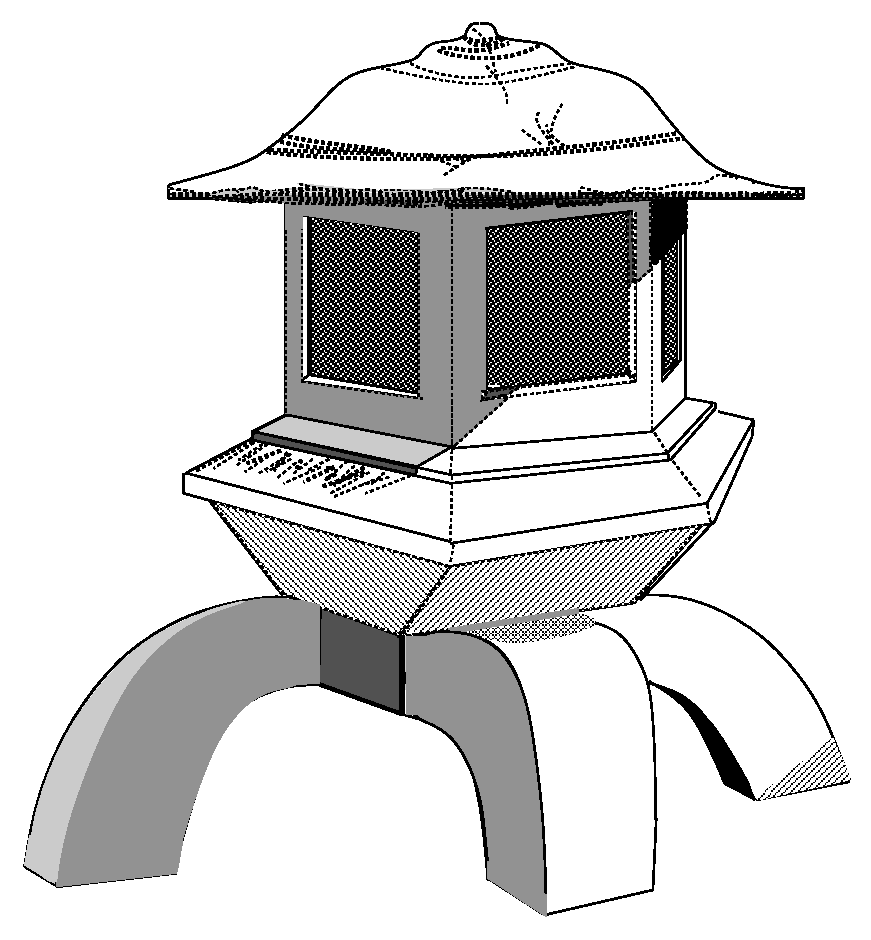
\includegraphics[width=3.8cm]{../Logo/lantern}
\end{center}


\vfill
\end{titlepage}

% To kick a blank page with no header
\thispagestyle{empty}
\cleardoublepage

%END LATEX

%HEVEA \begin{tabular}{l@{\hspace{5cm}}r}
%HEVEA {\bf [For \holnw{} \holnversion]} & \today\\
%HEVEA \end{tabular}
%HEVEA
%HEVEA \begin{center}
%HEVEA {\Huge\bf The HOL-Omega System}\\
%HEVEA {\LARGE \bf TUTORIAL TEASER}\\
%HEVEA \vspace{1cm}
%HEVEA \begin{toimage}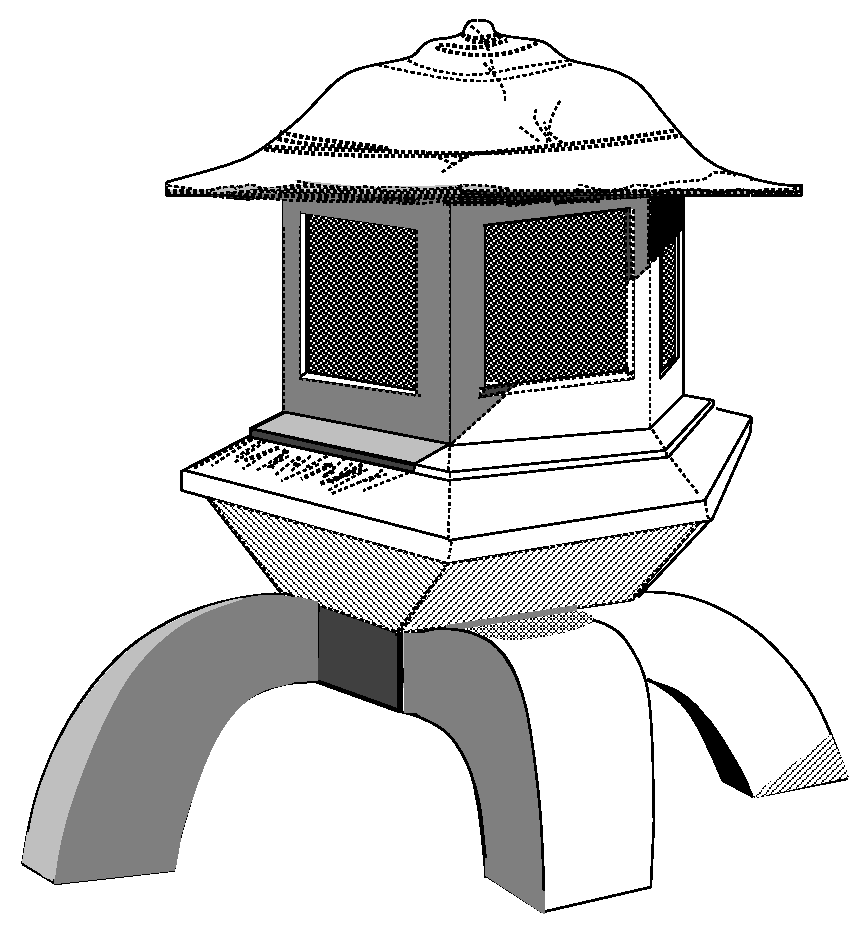
\epsfig{file=../Covers/LANTERN.ps,height=2.5in}\\
%HEVEA \end{toimage}\imageflush
%HEVEA \begin{tabular}{ccc}
%HEVEA University of Cambridge & \hspace*{10ex}DSTO\hspace*{10ex} & SRI International
%HEVEA \end{tabular}
%HEVEA \end{center}




%%% Local Variables:
%%% mode: latex
%%% TeX-master: "tutorial"
%%% End:
                  % tutorial teaser title page
%%   \chapter*{Preface}\markboth{Preface}{Preface}
\label{intro}

This volume contains a tutorial on the \HOL\ system.  It is one of three
documents making up the documentation for \HOL:

\begin{myenumerate}
\item \TUTORIAL: a tutorial introduction to \HOL.
\item \DESCRIPTION: a description of higher order logic,
the \ML\ programming language, and theorem proving methods in the \HOL\ system;
\item \REFERENCE: the reference documentation of the tools available in \HOL.
\end{myenumerate}

\noindent These three documents will be referred to by the short names (in
small slanted capitals) given above.

This document, \TUTORIAL, is intended to be the first item read by new users of
\HOL.  It provides a self-study introduction to the structure and use of the
system.  The tutorial is intended to give a `hands-on' feel for the way \HOL\
is used, but it does not systematically explain all the underlying principles
(\DESCRIPTION, explains these).  After working through \TUTORIAL\ the reader
should be capable of using \HOL\ for simple tasks, and should also be in a
position to consult the other two documents.

\section*{Getting started}

Chapter~\ref{install} explains how to get and install \HOL.  Once this is done,
the potential \HOL\ user should become familiar with the following subjects:

\begin{enumerate}
\item The programming meta-language \ML, and how to interact
with it through an editor.
\item The formal logic supported by 
the \HOL\ system (higher order logic) and its manipulation via \ML.
\item Forward proof and derived rules of inference.
\item Goal directed proof, tactics and tacticals.
\end{enumerate}

Chapters 1--5 introduce these topics. The remaining three chapters
contain examples of complete pieces of work.
\begin{itemize}
\item Chapter~\ref{parity}
consists of a worked example: the specification and
verification of a simple sequential parity checker.  The intention is
to   accomplish two things:
(i) to present a complete piece of work with \HOL; and
(ii) to give an idea of what it is like to use the \HOL\
system for a tricky proof.  

\item Chapter~\ref{tool} shows how a special purpose proof tool (a conjunction
normaliser) can be implemented and optimised. It illustrates methods for
`tuning' proof generating programs and discusses trade-offs between generality
and efficiency.

\item Chapter~\ref{binomial} is a proof of the Binomial Theorem in a ring.  It
is a medium sized worked example whose subject matter is probably more widely
known than any specific piece of hardware or software. The small amount of
algebra and mathematical notation needed to state and prove the Binomial
Theorem is presented; the notation is expressed in \HOL{}, and the
structure of the proof is outlined.

\end{itemize}

\noindent \TUTORIAL\ has been kept short so that new users of \HOL\ can get
going as fast as possible. Sometimes details have been simplified. It is
recommended that as soon as a topic in \TUTORIAL\ has been digested, the
relevant bits of \DESCRIPTION\ and \REFERENCE\ be studied.

\section*{Exercises}

The directory:

\begin{hol}\begin{verbatim}
   hol/Training/exercises
\end{verbatim}\end{hol}

\noindent contains exercises (with solutions) in the use of \HOL. It is
recommended that these exercises be studied in conjunction with reading
\TUTORIAL\ and \DESCRIPTION.

\section*{Courseware}

The  directory:

\begin{hol}\begin{verbatim}
   hol/Training/course
\end{verbatim}\end{hol}

\noindent contains the \LaTeX\ sources for an intensive course on \HOL\
developed by Tom Melham. These are intended to be a resource for anyone who
wishes to teach \HOL.

\section*{Case studies}

The previous version of \TUTORIAL\ contained a number of advanced case
studies. These are now separate documents in the directory:

\begin{hol}\begin{verbatim}
   hol/Training/studies
\end{verbatim}\end{hol}

\noindent The case studies in this directory are:

\begin{enumerate}
\item {\tt microprocessor}:  the specification and verification of a simple
microprocessor, due to Jeff Joyce ({\verb+joyce@cs.ubc.ca+}).
This case study illustrates the
state-of-the-art in an already mature area. Several new techniques are
illustrated, including the use of temporal logic embedded in \HOL\ for
reasoning about asynchronous processes.
\item {\tt protocols}: the specification and verification of a sliding window
protocol, due to Rachel Cardell-Oliver ({\verb+rco@cam.sri.com+}).
This case study shows a new and
rapidly evolving application of the \HOL\ system that is currently an
active area of research at Cambridge. There have been significant developments 
in this field since this study was written.
\item {\tt int\_mod}: modular arithmetic of integers
developed as an application of the group
theory library, due to Elsa Gunter ({\verb+elsa@research.att.com+}).
This case study
is a comprehensive
tutorial on how one might conduct mathematical proof in type theory.
It shows how to apply the abstract group theory library, which she
wrote, to the development of a particular mathematical theory (modular
arithmetic).  Her paper {\sl Doing Algebra in Simple Type Theory} is
included with the case study for the reader's convenience (it is also
to be published elsewhere).
\end{enumerate}

The case studies use different styles of proof in \HOL, different ways of
laying out \ML\ code, etc. These reflect the differing aesthetic tastes and
backgrounds of the authors. It is not intended that any of the styles is to be
considered `standard'.  There may eventually emerge a `Manual of Proof Style
for \HOL', but it would be premature to try to write one now. It is a
considerable virtue of Milner's \LCF\ approach to theorem proving that it so
smoothly accommodates such a wide variety of styles, and yet maintains complete
logical security.

The reader is warned that the case studies were developed for \HOL 88 Version
1.10 and it is possible that they will need to be modified to run in later
versions of \HOL.












                      % preface to entire tutorial
   \chapter*{Prologue}\markboth{Prologue}{Prologue}
\label{prologue}

This volume contains a short sample of material from the upcoming
tutorial on the \HOLW{} system.  The tutorial will be one of four
documents making up the documentation for \HOLW:

\begin{myenumerate}
\item \LOGIC: a formal description of the higher order logic
  implemented by the \HOLW{} system.
\item \TUTORIAL: a tutorial introduction to \HOLW, with case studies.
\item \DESCRIPTION: a detailed user's guide for the \HOLW{} system;
\item \REFERENCE: the reference manual for \HOLW.
\end{myenumerate}

This document provides a brief and light set of examples of using \HOLW{},
as an introduction, giving a taste of how the system might be used.
Like an appetizer to a main meal, it provides just a hint of
the sustenance to come.

\section*{Getting started}

Chapter~\ref{install} explains how to get and install \HOLW.
Then the new, additional
concepts and features of the \HOLW{} logic (higher order logic 
extended with System {\it F}, kinds, and ranks)
are casually demonstrated,
in chapter \ref{chap:appetizers}.

Chapter~\ref{chap:teaser_epilogue} briefly discusses some of the
examples distributed with \holnw{} in the \ml{examples/HolOmega} directory.

%\item Chapter~\ref{tool} shows how a special purpose proof tool (a
%  conjunction normaliser) can be implemented and optimised. It
%  illustrates methods for `tuning' proof generating programs and
%  discusses trade-offs between generality and efficiency.

%\item Chapter~\ref{binomial} is a proof of the Binomial Theorem in a
%  ring.  It is a medium sized worked example whose subject matter is
%  probably more widely known than any specific piece of hardware or
%  software. The small amount of algebra and mathematical notation
%  needed to state and prove the Binomial Theorem is presented; the
%  notation is expressed in \HOLW{}, and the structure of the proof is
%  outlined.

%\end{itemize}

\vspace{1cm}

%\noindent \TUTORIAL{} has been kept short so that new users of \HOLW{} can get
%going as fast as possible. Sometimes details have been simplified. It
%is recommended that as soon as a topic in \TUTORIAL\ has been
%digested, the relevant parts of \DESCRIPTION\ and \REFERENCE\ be
%studied.

%%% Local Variables:
%%% mode: latex
%%% TeX-master: "tutorial"
%%% End:
                      % prologue to teaser
   \chapter*{Riconoscimenti}\markboth{Riconoscimenti}{Riconoscimenti}

La maggior parte di \HOL\ � basato su codice scritto da---in ordine 
alfabetico---%
Hasan Amjad,
Richard Boulton,
Anthony Fox,
Mike Gordon,
Elsa Gunter,
John Harrison,
Peter Homeier,
G\'erard Huet (e altri presso l'istituto INRIA),
Joe Hurd,
Ramana Kumar,
Ken Friis Larsen,
Tom Melham,
Robin Milner,
Lockwood Morris,
Magnus Myreen,
Malcolm Newey,
Michael Norrish,
Larry Paulson,
Konrad Slind,
Don Syme,
Thomas T\"urk,
Chris Wadsworth,
e
Tjark Weber.
Molti altri hanno fornito parti del sistema, correzione di bug, ecc.

\subsection*{Edizione attuale}

L'edizione attuale di tutti e quattro i volumi (\LOGIC, \TUTORIAL,
\DESCRIPTION\ e \REFERENCE) � stata preparata da Michael Norrish e 
Konrad Slind. Altri contributi a questi volumi sono venuti da Hasan
Amjad, che ha sviluppato una libreria di controllo del modello, e ha scritto le sezioni 
che ne descrivono l'uso; Jens Brandt, che ha sviluppato e documentato una 
libreria per i numeri razionali; Anthony Fox, che ha formalizzato e 
documentato nuove teorie dei gruppi riguardanti i word e le librerie associate; Mike 
Gordon, che ha documentato le librerie per i BDD e SAT; Peter Homeier, 
che ha implementato e documentato la libreria quoziente; Joe Hurd, che 
ha aggiunto materiale sulla ricerca della dimostrazione nel primo ordine; e Tjark Weber, che ha scritto 
le librerie per le Teorie Modulo Soddisfacibilit�~(SMT) e le Formule Booleane 
Quantificate~(QBF).

\medskip

Il materiale nella terza edizione costituisce un'approfondita rielaborazione 
ed estensione delle edizioni precedenti, l'unico pezzo essenzialmente non 
alterato � la semantica di Andy Pitts (in \LOGIC), il che riflette il fatto 
che, nonostante il sistema \HOL\ abbia subito uno sviluppo e un miglioramento 
continuo, la logica di \HOL\ � rimasta inalterata dalla sua prima edizione 
(1988).

\newpage

\subsection*{Seconda edizione}

La seconda edizione di \REFERENCE\ � stato uno sforzo congiunto da parte del gruppo 
\HOL\ di Cambridge.

\subsection*{Prima edizione}

I tre volumi \TUTORIAL, \DESCRIPTION\ e \REFERENCE\ sono stati 
prodotti presso il Cambridge Research Center della SRI International con il 
supporto del DSTO Australia.

Il progetto di documentazione di \HOL\ fu gestito da Mike Gordon, che 
scrisse anche parti di \DESCRIPTION\ e \TUTORIAL\ usando del materiale basato su 
uno scritto originario che descriveva il sistema \HOL\footnote{M.J.C.\ Gordon, `HOL:
  a Proof Generating System for Higher Order Logic', in: {\it VLSI
    Specification, Verification and Synthesis\/}, edito da G.\
  Birtwistle e P.A.\ Subrahmanyam, (Kluwer Academic Publishers,
  1988), pp.\ 73--128.} e {\sl The ML Handbook\/}\footnote{{\sl The
    ML Handbook}, scritto inedito presso l'Inria da parte di Guy Cousineau, Mike
  Gordon, G\'erard Huet, Robin Milner, Larry Paulson and Chris
  Wadsworth.}. Altri che hanno contribuito a \DESCRIPTION\ includono Avra Cohn, 
che ha scritto del materiale su teoremi, regole, conversioni e tattiche, 
e ha anche composto l'indice (che fu battuto a macchina da Juanito Camilleri); 
Tom Melham, che ha scritto le sezioni che descrivono le definizioni di tipo, 
il concreto pacchetto dei tipi, e le tattiche di `risoluzione'; e Andy Pitts, 
che ha ideato la semantica a modelli insiemistici della logica di \HOL\ e ha scritto 
il materiale che la descrive.

Il documento originario usava macro \LaTeX\ fornite da Elsa
Gunter, Tom Melham e Larry Paulson. La battitura di tutti e tre 
i volumi fu gestita da Tom Melham. La copertina fu disegnata da Arnold
Smith, che us� una fotografia di una `lanterna da neve' presa da 
Avra Cohn (nel cui giardino risiede l'oggetto originale). John Van
Tassel ha composto l'immagine \LaTeX\ della lanterna.

Molte altre persone oltre a quelle elencate di sopra hanno contribuito nello sforzo della 
documentazione di \HOL\, sia fornendo materiale, sia inviando elenchi di errori nella prima 
edizione. Grazie a tutti coloro che hanno aiutato, e grazie al DSTO e all'SRI per il loro 
generoso supporto.




                 % global acknowledgements
   \tableofcontents

%   \newpage
%   \pagenumbering{arabic}                % arabic page numbers
%   \setcounter{page}{1}                  % start at page 1

   \chapter{Getting and Installing HOL-Omega}
\label{install}

This chapter describes how to get the \HOLW{} system and how to install
it.  It is generally assumed that some sort of Unix system is being
used, but the instructions that follow should apply {\it mutatis
  mutandis\/} to other platforms.  Unix is not a pre-requisite for
using the system. \HOLW{} may be run on PCs running Windows operating
systems from Windows~NT onwards (i.e., Windows~2000, XP and Vista are
also supported), as well as Macintoshes running Mac~OS~X.

\section{Getting HOL-Omega}

% The \HOLW{} system can be downloaded from
% % \url{http://hol.sourceforge.net}.
% \url{https://github.com/mn200/HOL} as part of the \HOL\ system. 
% % \HOLW\ is an extension of \HOL{-4}, and is backwards compatible with it.
\HOLW{} is part of the \HOL\ system.
% The \HOL\ system has several branches; branch {\tt HOL-Omega} is where
% development of the HOL-Omega theorem prover occurs.
The \HOL\ system has several branches; branch {\tt HOL-Omega} contains
the source of the HOL-Omega theorem prover.
The naming scheme for \holnw{}
releases is $\langle${\it name}$\rangle$-$\langle${\it
  number}$\rangle$; the release described here is \holnversion.

\HOL\ development uses the Git version control system.
Git is freely available from \texttt{http://git-scm.com/},
and is well described in the book {\it ProGit\/} by Scott Chacon.

A fresh copy of the current developer version of \HOLW\ may be checked out
into a fresh subdirectory called {\tt hol-omega} by the following Git command:
\begin{center}
\texttt{git clone -b HOL-Omega git://github.com/mn200/HOL.git hol-omega}
\end{center}

As a developer, to check out a fresh copy of \HOLW\ that one could
edit and write back to the github repository, one would set up a SSH key
with github and then do
\begin{center}
\texttt{git clone -b HOL-Omega git@github.com:mn200/HOL.git hol-omega}
\end{center}

\noindent
%To set up a SSH key with github, see
To set up a SSH key, see
%\begin{center}
\texttt{https://help.github.com/articles/generating-ssh-keys}.
%\end{center}

To become an \HOL\ developer and have write access to the github
repository, please contact one of the administrators listed at
\texttt{http://sourceforge.net/projects/hol/}.

\section{The {\tt hol-info} mailing list}

The \texttt{hol-info} mailing list serves as a forum for discussing
\HOLW{} and disseminating news about it.  If you wish to be on this
list (which is recommended for all users of \HOLW), visit
\url{http://lists.sourceforge.net/lists/listinfo/hol-info}.  This
web-page can also be used to unsubscribe from the mailing list.

\section{Installing HOL-Omega}

It is assumed that the \HOLW{} sources have been obtained and the
\texttt{tar} file unpacked into a directory \ml{hol-omega}.\footnote{You may
  choose another name if you want; it is not important.} The contents
of this directory are likely to change over time, but it should
contain the following:

\begin{center}
\begin{tabular}{|l|l|l|} \hline
\multicolumn{3}{|c|}{ } \\
\multicolumn{3}{|c|}{\bf Principal Files on the HOL-Omega Distribution Directory} \\
\multicolumn{3}{|c|}{ } \\
{\it File name} & {\it Description} & {\it File type}  \\ \hline
{\tt README} & Description of directory {\tt hol-omega} & Text\\
{\tt COPYRIGHT}& A copyright notice & Text\\
{\tt INSTALL} & Installation instructions & Text\\
{\tt tools} & Source code for building the system & Directory\\
{\tt bin} & Directory for HOL-Omega executables & Directory\\
{\tt sigobj} & Directory for \ML{} object files & Directory\\
{\tt src} & \ML{} sources of \HOLW & Directory\\
{\tt help} & Help files for \HOLW{} system & Directory\\
{\tt examples} & Example source files & Directory\\
\hline
\end{tabular}
\end{center}

The session in the box below shows a typical distribution directory.
The \HOLW{} distribution has been placed
in the directory {\small\tt /Users/palantir/hol-omega/}
on a Macintosh running OS X
% in the home directory of
for a user {\small\tt palantir}.

All sessions in this documentation will be displayed in boxes with a
number in the top right hand corner.  This number indicates whether
the session is a new one (when the number will be {\small\sl 1}) or
the continuation of a session started in an earlier box.
Consecutively numbered boxes are assumed to be part of a single
continuous session.  The Unix prompt for the sessions is
\texttt{\small \dol}, so lines beginning with this prompt were typed
by the user.  After entering the \HOLW{} system (see below), the user
is prompted with {\small\verb|-|} for an expression or command of the
\HOLW{} meta-language \ML; lines beginning with this are thus \ML\
expressions or declarations.  Lines not beginning with \texttt{\small
  \$} or {\small\verb|-|} are system output.  Occasionally, system
output will be replaced with a line containing {\small\verb|...|} when
it is of minimal interest. The meta-language \ML{} is introduced in
Chapter~\ref{ML}.

\setcounter{sessioncount}{0}
\begin{session}
% COPYRIGHT  bin/  examples/  INSTALL  src/
% README     doc/  help/      sigobj/  tools/
\begin{verbatim}
$ pwd
/Users/palantir/hol-omega
$ ls -F
COPYRIGHT   bin/          examples/   sigobj/       tools-poly/
INSTALL	    cleanall*     help/       src/
Manual/	    developers/   icon.gif*   std.prelude 
README      doc/          merging     tools/
\end{verbatim}
\end{session}

Now you will need to rebuild \HOLW{} from the sources.\footnote{It is
  possible that pre-built systems may soon be available from the
  web-page mentioned above.}

Before beginning you must have a current version of Moscow~ML or
Poly/ML\footnote{Poly/ML cannot be used with HOL-Omega on Windows.}.  In the
case of Moscow~ML, you must have version 2.01.  Moscow~ML is available
on the web from \url{http://www.dina.kvl.dk/~sestoft/mosml.html}.
Poly/ML is available from \url{http://polyml.org}. When you have your
ML system installed, and are in the root directory of the
distribution, the next step is to run \texttt{smart-configure}.  With
Moscow~ML, this looks like:

\begin{session}
\begin{alltt}
\dol mosml < tools/smart-configure.sml
Moscow ML version 2.01 (January 2004)
Enter `quit();' to quit.
- [opening file "tools/smart-configure-mosml.sml"]

HOL-Omega smart configuration.

Determining configuration parameters: OS mosmldir holdir
OS:                 macosx
mosmldir:           /Users/palantir/mosml/bin
holdir:             /Users/palantir/hol-omega
dynlib_available:   true

Configuration will begin with above values.  If they are wrong
press Control-C.
\end{alltt}
\end{session}

If you are using Poly/ML, then write
\begin{verbatim}
   poly < tools/smart-configure.sml
\end{verbatim}
instead.

Assuming you don't interrupt the configuration process, this will
build the \texttt{Holmake} and \texttt{build} programs, and move them
into the \texttt{hol-omega/bin} directory.  If something goes wrong at this
stage, consult Section~\ref{sec:editting-configure} below.

The next step is to run the \texttt{build} program.  This should
result in a great deal of output as all of the system code is compiled
and the theories built.  Eventually, a \HOLW{} system\footnote{Four
  \HOLW{} executables are produced: \textsf{hol}, \textsf{hol.noquote},
  \textsf{hol.bare} and \textsf{hol.bare.noquote}.  The first of these
  will be used for most examples in the \TUTORIAL{}.} is produced in
the \texttt{bin/} directory.

\begin{session}
\begin{alltt}
\dol bin/build
  ...
  ...
Uploading files to /Users/palantir/hol-omega/sigobj

Hol built successfully.
\dol
\end{alltt}
\end{session}


\subsection{Overriding \texttt{smart-configure}}
\label{sec:editting-configure}

If \texttt{smart-configure} is unable to guess correct values for the
various parameters (\texttt{holdir}, \texttt{OS} \etc) then you can
create a file called to provide correct values.  With Moscow~ML, this
should be \texttt{config-override} in the root directory of the HOL-Omega
distribution.  With Poly/ML, this should be \texttt{poly-includes.ML}
in the \texttt{tools-poly} directory. In this file, specify the
correct value for the appropriate parameter by providing an ML binding
for it.  All variables except \texttt{dynlib\_available} must be given
a string as a possible value, while \texttt{dynlib\_available} must be
either \texttt{true} or \texttt{false}.  So, one might write

\begin{session}
\begin{verbatim}
val OS = "unix";
val holdir = "/local/scratch/myholdir";
val dynlib_available = false;
\end{verbatim}
\end{session}

The \texttt{config-override} file need only provide values for those
variables that need overriding.

With this file in place, the \texttt{smart-configure} program will use
the values specified there rather than those it attempts to calculate
itself.  The value given for the \texttt{OS} variable must be one of
\texttt{"unix"}, \texttt{"linux"}, \texttt{"solaris"},
\texttt{"macosx"} or \texttt{"winNT"}.\footnote{The string
  \texttt{"winNT"} is used for Microsoft Windows operating systems
  that are at least as recent as Windows~NT.  This includes
  Windows~2000, XP and Vista.}

In extreme circumstances it is possible to edit the file
\texttt{tools/configure.sml} yourself to set configuration variables
directly.  (If you are using Poly/ML, you must edit
\texttt{tools-poly/configure.sml} instead.) At the top of this file
various incomplete SML declarations are present, but commented out.
You will need to uncomment this section (remove the \texttt{(*} and
\texttt{*)} markers), and provide sensible values.  All strings must
be enclosed in double quotes.

The \texttt{holdir} value must be the name of the top-level directory
listed in the first session above.  The \texttt{OS} value should be
one of the strings specified in the accompanying comment.

When working with Moscow~ML, the \texttt{mosmldir} value must be the
name of the directory containing the Moscow~ML binaries
(\texttt{mosmlc}, \texttt{mosml}, \texttt{mosmllex} etc).  When
working with Poly/ML, the \texttt{poly} string must be the path to the
\texttt{poly} executable that begins an interactive \ML{} session.
The \texttt{polymllibdir} must be a path to a directory that contains
the file \texttt{libpolymain.a}.

Subsequent values (\texttt{CC} and \texttt{GNUMAKE}) are needed for
``optional'' components of the system.  The first gives a string
suitable for invoking the system's C compiler, and the second
specifies a \textsf{make} program.

After editing, \texttt{tools/configure.sml} the lines above will look
something like:

\begin{session}
\begin{alltt}
\dol more configure.sml
  ...
val mosmldir:string = "/home/palantir/mosml";
val holdir :string  = "/home/palantir/hol-omega";
val OS :string      = "linux";
                           (* Operating system; choices are:
                                "linux", "solaris", "unix", "macosx",
                                "winNT"   *)

val CC:string       = "gcc";      (* C compiler                       *)
val GNUMAKE:string  = "make";     (* for bdd library and SMV          *)
val DEPDIR:string   = ".HOLMK";   (* where Holmake dependencies kept  *)
  ...
\dol
\end{alltt}
\end{session}

\noindent Now, at either this level (in the \texttt{tools} or
\texttt{tools-poly} directory) or at the level above, the script
\texttt{configure.sml} must be piped into the \ML{} interpreter (\ie,
\texttt{mosml} or \texttt{poly}).  For example,

\begin{session}
\begin{alltt}
\dol mosml < tools/configure.sml
Moscow ML version 2.01 (January 2004)
Enter `quit();' to quit.
- > val mosmldir = "/home/palantir/mosml" : string
  val holdir = "/home/palantir/hol-omega" : string
  val OS = "linux" : string
- > val CC = "gcc" : string
  ...
Beginning configuration.
Removing old quotation filter from bin/
Making tools/mllex/mllex.exe
Making bin/Holmake.
  ...
Making bin/build.
Making hol-mode.el (for Emacs/XEmacs)
Generating bin/hol.
Generating bin/hol.noquote.
  ...
Number of states = 170
Number of distinct rows = 90
Approx. memory size of trans. table = 23040 bytes
Analysing filter.sml
Compiling filter.sml
Compiling quote-filter.sml
  ...
Analysing selftest.sml
Quote-filter built
Setting up the muddy library Makefile.

Finished configuration!
\dol
\end{alltt}
\end{session}



%%% Local Variables:
%%% mode: latex
%%% TeX-master: "tutorial"
%%% End:
                       % intro: getting and installing hol
%%   \chapter{Introduzione a ML}
\label{ML}

Questo capitolo � una breve introduzione al meta-linguaggio \ML.
L'obiettivo � solo quello di dare una sensazione di come sia interagire con
il linguaggio. Si pu� trovare un'introduzione pi� dettagliata
in numerosi libri di testo e pagine web; si veda per esempio l'elenco delle risorse
sulla home page
di MoscowML\footnote{\url{http://www.dina.kvl.dk/~sestoft/mosml.html}},
o le FAQ
\texttt{comp.lang.ml}\footnote{\url{http://www.faqs.org/faqs/meta-lang-faq/}}.

\section{Come interagire con ML}

\ML{} � un linguaggio di programmazione interattivo come il Lisp. Al livello
dell'interprete si possono valutare espressioni ed eseguire dichiarazioni. Le prime
risultano nella stampa a schermo del valore dell'espressione e del suo tipo, le seconde
nel binding di un valore a un nome.

Un modo standard di interagire con \ML{} � quello di configurare lo schermo
della workstation in modo tale che ci siano due finestre:
\begin{myenumerate}
\item Una finestra di modifica in cui i comandi \ML{} sono inizialmente battuti
  e registrati.
\item Una finestra shell (o l'equivalente non-Unix) che � usata per
  valutare i comandi.
\end{myenumerate}

\noindent
Un modo comune per ottenere questo � lavorare all'interno di \ml{Emacs} con una
finestra di testo e una finestra shell.

Dopo ave battuto un comando sulla finestra di modifica (testo) esso pu� essere
trasferito alla shell e valutato in \HOL{} con un `copia e incolla'. In
\ml{Emacs} questo si ottiene copiando il testo in un buffer e poi facendo il
suo `yanking' nella shell. Il vantaggio di lavorare con un editor �
che se il comando ha un errore, allora il testo pu� essere modificato semplicemente
e usato di nuovo; inoltre esso salva i comandi in un file che pu� poi
essere usato di nuovo pi� avanti (attraverso un caricamento batch). In \ml{Emacs}, la finestra
di shell registra anche la sessione, inclusi sia l'input dell'utente
sia la risposta del sistema. Le sessioni in questo tutorial sono state prodotte
in questo modo. Queste sessioni sono divise in segmenti mostrati in riquadri
con un numero sul loro angolo superiore destro (per indicare la loro
posizione nella sessione completa).

Le interazioni in questi riquadri dovrebbero essere intese operare in
sequenza. Per esempio, si assume che i binding delle variabili fatte in box precedenti
persistano nei successivi. Per entrare nel sistema \HOL{} si
digita {\small\verb|hol|} o {\small\verb|hol.noquote|} in Unix,
eventualmente preceduti dall'informazione del percorso se la directory bin del sistema
\HOL{} non � nel proprio percorso. Il sistema \HOL{} quindi
stampa un messaggio di sign-on e ci colloca all'interno di \ML. Il prompt \ML{} �
{\small\verb|-|}, perci� le righe cominciano con {\small\verb|-|} sono quelle digitate
dall'utente e le altre righe sono le risposte del sistema.

  Qui, come nelle altre parti del \TUTORIAL{}, assumeremo che si stia usando
  {\small\verb|hol|}.

\setcounter{sessioncount}{0}
\begin{session}\begin{alltt}
\$ bin/hol

-----------------------------------------------------------------
       HOL-4 [\holnsversion (built Fri Apr 12 15:34:35 2002)]

       For introductory HOL help, type: help "hol";
-----------------------------------------------------------------

[loading theories and proof tools ************* ]
[closing file "/local/scratch/mn200/Work/hol98/tools/end-init-boss.sml"]
- 1 :: [2,3,4,5];
> val it = [1, 2, 3, 4, 5] : int list
\end{alltt}
\end{session}

L'espressione \ML{} {\small\verb|1 :: [2,3,4,5]|} ha la forma $e_1\
op\ e_2$ dove $e_1$ � l'espressione {\small\verb|1|} (il cui valore
� l'intero $1$), $e_2$ � l'espressione {\small\verb|[2,3,4,5]|}
(il cui valore � una lista di quattro interi) e $op$ � l'operatore
infisso `{\small\verb|::|}' che � come la funzione del Lisp {\it cons}.
Altre funzioni di elaborazione di liste includono {\small\verb|hd|} ($car$ in
Lisp), {\small\verb|tl|} ($cdr$ in Lisp) e {\small\verb|null|}
($null$ in Lisp). Il punto e virgola `{\small\verb|;|}' termina una
frase complessiva. La risposta del sistema � mostrata sulla linea che comincia
con il prompt {\small\verb|>|}. Essa consiste del valore
dell'espressione seguito, dopo un segno di due punti, dal suo tipo. Il type checker di \ML{}
deduce il tipo delle espressioni usando metodi inventati da Robin Milner
\cite{Milner-types}. Il tipo {\small\verb|int list|} � il tipo delle
`liste di interi'; {\small\verb|list|} � un operatore di tipo unario.
Il sistema di tipi di \ML{} � molto simile al sistema di tipi della
logica \HOL{} che � spiegata nel Capitolo~\ref{HOLlogic}.

Il valore dell'ultima espressione valutata dal top level \ML{} � sempre
memorizzata in una variabile chiamata {\small\verb|it|}.

\begin{session}
\begin{verbatim}
- val l = it;
> val l = [1, 2, 3, 4, 5] : int list

- tl l;
> val it = [2, 3, 4, 5] : int list

- hd it;
> val it = 2 : int

- tl(tl(tl(tl(tl l))));
> val it = [] : int list
\end{verbatim}
\end{session}

Seguendo gli standard del $\lambda$-calcolo, l'applicazione di una
funzione $f$ a un argomento $x$ pu� essere scritta senza parentesi come $f\
x$ (bench� � permesso anche
il pi� convenzionale $f${\small\verb|(|}$x${\small\verb|)|}). L'espressione
$f\ x_1\ x_2\ \cdots\ x_n$ abbrevia l'espressione
meno intelligibile {\small\verb|(|}$\cdots${\small\verb|((|}$f\ x_1$%
{\small\verb|)|}$x_2${\small\verb|)|}$\cdots${\small\verb|)|}$x_n$
(l'applicazione di funzione � associativa a sinistra).

Le dichiarazioni hanno la forma {\small\verb|val |}$x_1${\small\verb|=|}$e_1${\small\verb| and |}$\cdots
${\small\verb| and |}$x_n${\small\verb|=|}$e_n$ e hanno l'effetto che il valore di
ogni espressione $e_i$ venga legato al nome $x_i$.

\begin{session}
\begin{verbatim}
- val l1 = [1,2,3] and l2 = ["a","b","c"];
> val l1 = [1, 2, 3] : int list
  val l2 = ["a", "b", "c"] : string list
\end{verbatim}
\end{session}

Espressioni \ML{} come {\small\verb|"a"|}, {\small\verb|"b"|},
{\small\verb|"foo"|} \etc\ sono {\it stringhe\/} e hanno il tipo
{\small\verb|string|}. Qualsiasi sequenza di caratteri {\small ASCII} pu�
essere scritta tra virgolette\footnote{I caratteri di nuova riga devono essere scritti come
  \ml{$\backslash$n}, e le virgolette come \ml{$\backslash$"}.}. La funzione
{\small\verb|explode|} divide una stringa in una lista di caratteri
singoli, che sono scritti come stringhe di un singolo carattere, con
anteposto un carattere {\small\verb|#|}.

\begin{session}
\begin{verbatim}
- explode "a b c";
> val it = [#"a", #" ", #"b", #" ", #"c"] : char list
\end{verbatim}
\end{session}

Un'espressione della forma
{\small\verb|(|}$e_1${\small\verb|,|}$e_2${\small\verb|)|} viene valutata
a una coppia dei valori di $e_1$ e $e_2$. Se $e_1$ ha il tipo
$\sigma_1$ e $e_2$ ha il tipo $\sigma_2$ allora
{\small\verb|(|}$e_1${\small\verb|,|}$e_2${\small\verb|)|} ha il tipo
$\sigma_1${\small\verb|*|}$\sigma_2$. Il primo e il secondo componente
di una coppia possono essere estratti con le funzioni \ML{} {\small\verb|#1|}
e {\small\verb|#2|} rispettivamente. Se una tupla ha pi� di due componenti,
il suo $n$-esimo componente pu� essere estratto con una funzione
{\small\verb|#|$n$}.

I valori {\small\verb|(1,2,3)|}, {\small\verb|(1,(2,3))|} e
{\small\verb|((1,2), 3)|} sono tutti distinti e hanno i tipi
\linebreak{} {\small\verb|int * int * int|}, {\small\verb|int * (int * int)|} and
{\small\verb|(int * int) * int|} rispettivamente.

\begin{session}
\begin{verbatim}
- val triple1 = (1,true,"abc");
> val triple1 = (1, true, "abc") : int * bool * string
- #2 triple1;
> val it = true : bool

- val triple2 = (1, (true, "abc"));
> val triple2 = (1, (true, "abc")) : int * (bool * string)
- #2 triple2;;
> val it = (true, "abc") : bool * string
\end{verbatim}
\end{session}

\noindent L'espressioni \ML{} {\small\verb|true|} e {\small\verb|false|}
denotano i due valori di verit� di tipo {\small\verb|bool|}.

I tipi \ML{} possono contenere {\it variabili di tipo\/} {\small\verb|'a|},
{\small\verb|'b|}, {\small\verb|'c|}, \etc\ Tali tipi sono chiamati {\it
polimorfici\/}. Una funzione con un tipo polimorfico dovrebbe essere pensata come
se possedesse tutti i tipi che si possono ottenere sostituendo le variabili di tipo con dei tipi.
Questo � illustrato di sotto con la funzione {\small\verb|zip|}.

Le funzioni sono definite con dichiarazioni della forma {\small\verb|fun|}$\ f\
v_1\ \ldots\ v_n$ \ml{=} $e$ dove ciascuna $v_i$ � o una variabile o un pattern
composto di variabili.

La funzione {\small\verb|zip|}, di sotto, converte una coppia di liste
{\small\verb|([|}$x_1${\small\verb|,|}$\ldots${\small\verb|,|}$x_n$%
{\small\verb|], [|}$y_1${\small\verb|,|}$\ldots${\small\verb|,|}$y_n$%
{\small\verb|])|} in una lista di coppie
{\small\verb|[(|}$x_1${\small\verb|,|}$y_1${\small\verb|),|}$\ldots$%
{\small\verb|,(|}$x_n${\small\verb|,|}$y_n${\small\verb|)]|}.

\begin{session}
\begin{verbatim}
- fun zip(l1,l2) =
    if null l1 orelse null l2 then []
    else (hd l1,hd l2) :: zip(tl l1,tl l2);
> val zip = fn : 'a list * 'b list -> ('a * 'b) list

- zip([1,2,3],["a","b","c"]);
> val it = [(1, "a"), (2, "b"), (3, "c")] : (int * string) list
\end{verbatim}
\end{session}

Le funzioni possono essere {\it curried\/}, \ie\ prendono i lori argomenti `uno alla volta'
al posto che come una tupla. Questo � illustrato con la funzione
{\small\verb|curried_zip|} di sotto:

\begin{session}
\begin{verbatim}
- fun curried_zip l1 l2 = zip(l1,l2);
> val curried_zip = fn : 'a list -> 'b list -> ('a * 'b) list

- fun zip_num l2 = curried_zip [0,1,2] l2;
> val zip_num = fn : 'a list -> (int * 'a) list

- zip_num ["a","b","c"];
> val it = [(0, "a"), (1, "b"), (2, "c")] : (int * string) list
\end{verbatim}
\end{session}

La valutazione di un'espressione o {\it ha successo\/} o {\it
  fallisce\/}. Nel primo caso, la valutazione restituisce un valore; nel
secondo caso la valutazione � interrotta ed � sollevata
un'\emph{eccezione}. Questa eccezione � passata a qualunque cosa abbia invocato la valutazione.
Questo contesto pu� o propagare il fallimento (questo � il default) o
pu� {\it gestirlo\/}. Queste due possibilit� sono illustrate di sotto.
La gestione di un'eccezione � un'espressione della forma
$e_1${\small\verb| handle _ => |}$e_2$. Un'espressione di questa forma �
valutata valutando per prima cosa $e_1$. Se la valutazione ha successo (\ie\
non fallisce) allora il valore dell'intera espressione � il valore di
$e_1$. Se la valutazione di $e_1$ ha sollevato un'eccezione, allora il valore
dell'intera espressione � ottenuto valutando $e_2$.\footnote{Questa
  descrizione della gestione dell'eccezioni � di fatto una semplificazione grossolana
	del modo in cui le eccezioni possono essere gestite in \ML{}; si consulti un testo appropriato
	per una spiegazione migliore.}.

\begin{session}
\begin{verbatim}
- 3 div 0;
! Uncaught exception:
! Div

- 3 div 0 handle _ => 0;
> val it = 0 : int
\end{verbatim}
\end{session}

Le sessioni di sopra sono sufficienti per dare un idea dell'\ML. Nel prossimo
capitolo, sar� introdotta la logica supportata dal sistema \HOL{} (la logica di
ordine superiore), insieme con gli strumenti all'interno di \ML{} per
manipolarla.

%%% Local Variables:
%%% mode: latex
%%% TeX-master: "tutorial"
%%% End:
                          % intro to ml
%%   \chapter{The HOL Logic}
\label{HOLlogic}

The \HOL\  system  supports {\it  higher order  logic}.   This is  a version of
predicate calculus with three main extensions:

\begin{itemize}
\item Variables can range over functions and predicates
(hence `higher order').
\item The logic is {\it typed}.
\item There is no separate syntactic category of {\it formulae\/}
(terms of type \ml{bool} fulfill their role).
\end{itemize}

\section{Overview of higher order logic}

It is assumed the reader is familiar with predicate logic.  The syntax
and semantics of the particular logical system supported by \HOL\ is
described in detail in \DESCRIPTION.  The table below summarizes the
notation used.

\begin{center}
\begin{tabular}{|l|l|l|l|} \hline
\multicolumn{4}{|c|}{ } \\
\multicolumn{4}{|c|}{\bf Terms of the HOL Logic} \\
\multicolumn{4}{|c|}{ } \\
{\it Kind of term} & {\it \HOL\ notation} &
{\it Standard notation} &
{\it Description} \\ \hline
 & & & \\
Truth & {\small\verb|T|} & $\top$ & {\it true}\\ \hline
Falsity & {\small\verb|F|} & $\bot$ & {\it false}\\ \hline
Negation & {\small\verb|~|}$t$ & $\neg t$ & {\it not}$\ t$\\ \hline
Disjunction & $t_1${\small\verb|\/|}$t_2$ & $t_1\vee t_2$ &
$t_1\ ${\it or}$\ t_2$ \\ \hline
Conjunction & $t_1${\small\verb|/\|}$t_2$ & $t_1\wedge t_2$ &
$t_1\ ${\it and}$\ t_2$ \\ \hline
Implication & $t_1${\small\verb|==>|}$t_2$ & $t_1\imp t_2$ &
$t_1\ ${\it implies}$\ t_2$ \\ \hline
Equality & $t_1${\small\verb|=|}$t_2$ & $t_1 = t_2$ &
$t_1\ ${\it equals}$\ t_2$ \\ \hline
$\forall$-quantification & {\small\verb|!|}$x${\small\verb|.|}$t$ &
$\uquant{x}t$ & {\it for\ all\ }$x: t$ \\ \hline
$\exists$-quantification & {\small\verb|?|}$x${\small\verb|.|}$t$ &
$\equant{x}\ t$ & {\it for\ some\ }$x: t$ \\ \hline
$\hilbert$-term & {\small\verb|@|}$x${\small\verb|.|}$t$ &
$\hquant{x}t$ & {\it an}$\ x\ ${\it such\ that:}$\ t$ \\ \hline
Conditional & {\small\verb|(if|} $t$ {\small\verb|then|} $t_1$
              {\small\verb|else|} $t_2${\small\verb|)|} &
$(t\rightarrow t_1, t_2)$ & {\it if\ }$t${\it \ then\ }$t_1${\it\ else\ }$t_2$
 \\ \hline
\end{tabular}
\end{center}\label{logic-table}

\paragraph{Note on HOL example sessions}
All of the examples below assume that the user is running
\texttt{hol.unquote}, the executable for which is in the \texttt{bin/}
directory along with that for \texttt{hol}.  Further, the user needs
to execute the following commands before starting the sessions below:
\setcounter{sessioncount}{0}
\begin{session}
\begin{verbatim}
- app load ["arithmeticTheory", "pairTheory", "Psyntax"];
> val it = () : unit
- open Psyntax;
\end{verbatim}
\end{session}

\bigskip

Terms of the \HOL\ logic are represented in \ML\ by an {\it abstract
  type\/}\footnote{Abstract types appear to the user as primitive
  types with a collection of operations; they are described in
  \DESCRIPTION} called {\small\verb|term|}. They are normally input
between double back-quote marks.  For example, the expression
{\small\verb|``x /\ y ==> z``|} evaluates in \ML\ to a term representing
{\small\verb|x|}$\wedge${\small\verb|y|}$\Rightarrow${\small\verb|z|}.
Terms can be manipulated by various built-in \ML\ functions. For
example, the \ML\ function \ml{dest\_imp} with \ML\ type
{\small\verb|term -> term * term|} splits an implication into a pair
of terms consisting of its antecedent and consequent, and the \ML\
function \ml{dest\_conj} of type {\small\verb|term -> term * term|}
splits a conjunction into its two conjuncts.


\setcounter{sessioncount}{1}
\begin{session}
\begin{verbatim}
- ``x /\ y ==> z``;
> val it = ``x /\ y ==> z`` : term

- dest_imp it;
> val it = (``x /\ y``, ``z``) : term * term

- dest_conj(#1 it);
> val it = (``x``, ``y``) : term * term
\end{verbatim}
\end{session}

Terms of the \HOL\ logic are quite similar to \ML\ expressions, and
this can at first be confusing.  Indeed, terms of the logic have types
similar to those of \ML\ expressions.  For example,
{\small\verb|``(1,2)``|} is an \ML\ expression with \ML\ type
{\small\verb|term|}.  The \HOL\ type of this term is
{\small\verb|num # num|}.  By contrast, the \ML\ expression
{\small\verb|(``1``, ``2``)|} has type {\small\verb|term * term|}.

The types of \HOL\ terms form an \ML\ type called
{\small\verb|hol_type|}.  Types are usually input by applying the
parsing functionExpressions having the form
{\small\verb|``: |}$\cdots${\small\verb| ``|} evaluate to logical
types.
The built-in function {\small\verb|type_of|} has \ML\ type
{\small\verb|term->type|} and returns the logical type of a term.

\begin{session}
\begin{verbatim}
- ``(1,2)``;
> val it = ``(1,2)`` : term

- type_of it;
> val it = ``:num # num`` : hol_type

- (``1``, ``2``);
> val it = (``1``, ``2``) : term * term

- type_of(#1 it);
> val it = ``:num`` : hol_type
\end{verbatim}
\end{session}

To try to minimise confusion between the logical types of \HOL\ terms and
the \ML\ types of \ML\ expressions, the former will be referred to as {\it object
language types\/} and the latter as {\it meta-language types\/}.  For example,
{\small\verb|``(1,T)``|} is an \ML\ expression that has meta-language type
{\small\verb|term|} and evaluates to a term with object language type
{\small\verb|``:num#bool``|}.


\begin{session}
\begin{verbatim}
- ``(1,T)``;
> val it = ``(1,T)`` : term

- type_of it;
> val it = ``:num * bool`` : hol_type
\end{verbatim}
\end{session}

\HOL\ terms can be input using explicit {\it quotation\/}, as above, or
they can be constructed using \ML\ constructor functions. The function
{\small\verb|mk_var|} constructs a variable from a string and a type.  In
the example below, three variables of type {\small\verb|bool|} are
constructed.  These are used later.

\begin{session}
\begin{verbatim}
- val x = mk_var("x", ``:bool``)
  and y = mk_var("y", ``:bool``)
  and z = mk_var("z", ``:bool``);
> val x = ``x`` : term
  val y = ``y`` : term
  val z = ``z`` : term
\end{verbatim}
\end{session}

The constructors {\small\verb|mk_conj|} and {\small\verb|mk_imp|} construct
conjunctions and implications respectively.

\begin{session}
\begin{verbatim}
- val t = mk_imp(mk_conj(x,y),z);
> val t = ``x /\ y ==> z`` : term
\end{verbatim}
\end{session}

\section{Terms}

There are only four different kinds of terms:
\begin{enumerate}
\item Variables.
\item Constants.
\item Function applications: \ml{``$t_1$\ $t_2$``}.
\item $\lambda$-abstractions: {\small\verb|``\|}$x$\ml{.}$t$\ml{``}.
\end{enumerate}

Both variables and constants have a name and a type; the difference is
that constants cannot be bound by quantifiers, and their type is fixed
when they are declared (see below). The type checking algorithm uses
the types of constants to infer the types of variables in the same
quotation. If there is not enough type information type variables will
be guessed:

\begin{session}\begin{verbatim}
- ``~x``;
val it = ``~x`` : term

- ``x``;
<<HOL message: inventing new type variable names: 'a.>>
> val it = ``x`` : Term.term
- type_of it;
> val it = ``:'a`` : hol_type
\end{verbatim}\end{session}

    In the first case, the \HOL\ type checker used the known type
    \ml{bool->bool} of {\small\verb|~|} to deduce that the variable
    \ml{x} must have type \ml{bool}.  In the second case, it cannot
    deduce the type of \ml{x}.  The default `scope' of type
    information for type checking is a single quotation, so a type in
    one quotation cannot affect the type-checking of another.  If
    there is not enough contextually-determined type information to
    resolve the types of all variables in a quotation, then the system
    will guess different type variables for all the unconstrained
    variables.  Alternatively, it is possible to explicitly indicate
    the required types by using \ml{``$term$:$type$``} as illustrated
    below.

\begin{session}\begin{verbatim}
- ``(x,y)``;
<<HOL message: inventing new type variable names: 'a, 'b.>>
> val it = ``(x,y)`` : term
- type_of it;
> val it = ``:'a # 'b`` : hol_type

- ``x:num``;
> val it = ``x`` : term
- type_of it;
> val it = ``:num`` : hol_type
\end{verbatim}\end{session}

    Functions have types of the form \ml{$\sigma_1$->$\sigma_2$},
    where $\sigma_1$ and $\sigma_2$ are the types of the domain and
    range of the function, respectively.

\begin{session}\begin{verbatim}
- type_of ``$==>``;
> val it = ``:bool -> bool -> bool`` : hol_type

- type_of ``$+``;
> val it = ``:num -> num -> num`` : hol_type
\end{verbatim}\end{session}

\noindent Both \ml{+} and \ml{==>} are infixes, so their use in
contexts where they are not being used as such requires their
prefixing by the \texttt{\$}-sign.  This is analogous to the way in
which \texttt{op} is used in \ML. The session below illustrates the
use of these constants as infixes; it also illustrates object language
versus meta-language types.

\begin{session}\begin{verbatim}
- ``(x + 1, t1 ==> t2)``;
> val it = ``(x + 1,t1 ==> t2)`` : term

- type_of it;
> val it = ``:num # bool`` : hol_type

- (``x=1``, ``t1==>t2``);
> val it = (``x = 1``, ``t1 ==> t2``) : term * term

- (type_of (#1 it), type_of (#2 it));
> val it = (``:bool``, ``:bool``) : hol_type * hol_type
\end{verbatim}\end{session}

\noindent The types of constants are declared in {\it theories}.  This is
described later.

An application $t_1\ t_2$ is badly typed if $t_1$ is not a function:

\begin{session}\begin{verbatim}
- ``1 2``;

Type inference failure: unable to infer a type for the application of

(1 :num)

to

(2 :num)

unification failure message: unify failed
! Uncaught exception:
! HOL_ERR <poly>
\end{verbatim}\end{session}

\noindent or if it is a function, but $t_2$ is not in its range:

\begin{session}\begin{verbatim}
- ``~1``;

Type inference failure: unable to infer a type for the application of

$~

to

(1 :num)

unification failure message: unify failed
! Uncaught exception:
! HOL_ERR <poly>
\end{verbatim}\end{session}

    As before, the dollar in front of {\small\verb|~|} indicates that
    the constant has a special syntactic status (in this case a
    non-standard precedence). Putting {\small\verb|$|} in front of any
    symbol causes the parser to ignore any special syntactic status
    (like being an infix) it might have.

\begin{session}\begin{verbatim}
- ``$==> t1 t2``;
> val it = ``t1 ==> t2`` : term
- ``$/\ t1 t2``;
> val it = ``t1 /\ t2`` : term
\end{verbatim}\end{session}

    Lambda-terms, or $\lambda$-terms, denote functions. The symbol
    `{\small\verb|\|}' is used as an {\small ASCII} approximation to
    $\lambda$.  Thus `{\small\verb|\|}$x$\ml{.}$t$' should be read as
    `$\lquant{x}t$'. For example, {\small\verb|"\x. x+1"|} is a term
    that denotes the function $n\mapsto n{+}1$.

\begin{session}\begin{verbatim}
- ``\x. x + 1``;
> val it = ``\x. x + 1`` : term

- type_of it;
> val it = ``:num -> num`` : hol_type
\end{verbatim}\end{session}

The two most important quantifiers are \ml{!} and \ml{?}, universal
and existential quantifiers.  The logical statement that every number
is either even or odd might be phrased as
{\small\verb|!n. (n MOD 2 = 1) \/ (n MOD 2 = 0)|}, while the statement
of Euclid's result about the infinitude of primes is:
{\small\verb|!n. ?p. prime p /\ p > n|}






%%% Local Variables:
%%% mode: latex
%%% TeX-master: "tutorial"
%%% End:
                       % the HOL logic and intro to HOL proof
   \chapter{HOL-Omega Appetizers}\label{chap:appetizers}

% Whereas the previous chapter covered the classical \HOL{} logic,
This chapter will introduce the \HOLW{} logic, with the idea of
motivating it by a series of examples.  These examples are
only discussed superficially, to showcase the new ideas,
and not all details are pursued.
A more complete description of the \HOLW{} extensions is provided in
the next chapter in the tutorial.
But these are presented as appetizers,
to lightly show how the new features might be used to good effect.
% Some of these were inspired by the examples collected by Gabriel Scherer\footnote{
% {\tt http://blog.huoc.org/higher-rank-polymorphism.html}}.


\section{Collections}

To begin, \HOL{} is blessed with a number of different types in the logic that
represent different varieties of collections, like lists, sets, and bags. These
are polymorphic types, written e.g. $\alpha$ {\tt list}, where $\alpha$ is the
type of the elements of the list. All these collections are similar, in that they
all have an empty collection, they all have a way to insert a new element into
a collection, they all have a way to measure the size of a collection, etc.

Suppose one wanted to represent the notion of a collection as an abstraction
of the normal notions of a set or a list.  In \HOL{} there is no natural way to
do this, but in \HOLW{} one could use a type operator variable to stand for the
various collection types, and then create a record of some of
the normal functions used on collections, as follows.

\begin{session}
\begin{verbatim}
- new_theory "appetizers";
<<HOL message: Created theory "appetizers">>
> val it = () : unit
> set_trace "Unicode" 0;
val it = () : unit

- Hol_datatype `collection_ops =
     <| empty  : 'x 'col;
        insert : 'x -> 'x 'col -> 'x 'col;
        length : 'x 'col -> num |>`;
<<HOL message: Defined type: "collection_ops">>
> val it = () : unit
\end{verbatim}
\end{session}
Here we have used the type variable \texttt{'col} as a variable
to stand for the type operator we are talking about, whether \texttt{list},
\texttt{option}, or some other type.
In \HOL, type variables can only stand for entire types, like \texttt{num list},
but not type operators like just \texttt{list}.
But here, \texttt{'col} is being used as a function on types,
that takes a type \texttt{'x}, the type of the elements of the collection,
and returns a type \texttt{'x 'col}, the type of collections of such elements.
%While not present in \HOL{}, such type operator variables are made available in \HOLW{}.
Such type operator variables are one of the new features of \HOLW{}.

Both \texttt{'col} and \texttt{'x} are free type variables in this definition, so
the type being defined takes two arguments, e.g., \texttt{('col, 'x)collection\_ops}.
The order of the two arguments is by alphabetical order.

Now we can describe lists as collections:
\begin{session}
\begin{verbatim}
- val list_ops = Define
     `list_ops = <|empty := []:'a list; insert := CONS; length := LENGTH|>`;
Definition has been stored under "list_ops_def"
> val list_ops =
    |- list_ops = <|empty := []; insert := CONS; length := LENGTH|> : thm

- type_of ``list_ops``;
<<HOL message: inventing new type variable names: 'a>>
> val it =
    ``:(list, 'a) collection_ops``
     : hol_type
\end{verbatim}
\end{session}
The type of this collection is \texttt{(list, 'a) collection\_ops}.
The first argument is the type \texttt{list}, here being used without any type argument
of its own.  This is meaningful in \HOLW{}, although it may look weird to \HOL{} users
who are used to always seeing \texttt{list} with an argument, like \texttt{num list} or
\texttt{'a list}.  But here \texttt{list} is itself an argument, albeit a type operator
alone, replacing \texttt{'col} in the definition of \texttt{collection\_ops} above.

Here are sets described as collections:
\begin{session}
\begin{verbatim}
- val set_ops = Define
     `set_ops = <|empty := {}:'a set; insert := $INSERT; length := CARD|>`;
Definition has been stored under "set_ops_def"
> val set_ops = |- set_ops = <|empty := {}; insert := $INSERT; length := CARD|>
     : thm

- type_of ``set_ops``;
<<HOL message: inventing new type variable names: 'b>>
> val it =
    ``:(\'a. 'a -> bool, 'b) collection_ops``
     : hol_type
\end{verbatim}
\end{session}
Note that the first argument to this set collection type is
\verb|\|\texttt{'a.~'a~->~bool}. This is an {\it abstraction type}, similar to
the normal lambda abstraction in terms, but this abstraction is within the type
language of \HOLW.  The scope of the lambda binding of \texttt{'a} in the type
above is up to but not including the comma, which ends the first type argument.

% The second argument to this type is \texttt{'a}, which is distinct from the
% \texttt{'a} being used in the first argument.  The second argument is a free type
% variable, whereas the \texttt{'a} that appears twice within the first argument is
% a bound type variable.  These two variables are completely different variables and
% should not be confused with each other, just as the variables \texttt{x}
% which appear in \verb|\|\texttt{x.x+1} and in \texttt{2*x} are different
% variables.

But, you may ask, why does this type abstraction \verb|\|\texttt{'a.~'a~->~bool}
appear in this collection type?  The reason is that the type of sets in \HOL,
\texttt{'a set}, is actually a type abbreviation, not a real type. It is a feature
of the parser and prettyprinter, not the actual logic as such.  The abbreviation
\texttt{'a set} stands for the real type \texttt{'a -> bool}. The \HOLW{} system
figures out the appropriate type to substitute for the type argument \texttt{'col}
to create the type \texttt{'a -> bool},
% and that type is \verb|\|\texttt{'a.~'a~->~bool}.
and the substitution is [\texttt{'col} $\mapsto$ \verb|\|\texttt{'a.~'a~->~bool}].
The type resulting from the substitution
is \texttt{'a~(}\verb|\|\texttt{'a.~'a~->~bool)} (in postfix notation),
which is equivalent to \texttt{'a~->~bool} through type beta-reduction.

\HOL{} contains not only lists and sets, but also bags, which are sometimes
called multisets. Bags are like sets which can include multiple copies of
its elements, whereas sets can only contain a single copy of each.
Here are bags described as collections:
\begin{session}
\begin{verbatim}
- load "bagLib";
...
- val bag_ops = Define
     `bag_ops = <| empty := {||}:'a bag; insert := BAG_INSERT;
                   length := BAG_CARD|>`;
Definition has been stored under "bag_ops_def"
> val bag_ops =
    |- bag_ops = <|empty := {||}; insert := BAG_INSERT; length := BAG_CARD|> :
  thm

- type_of ``bag_ops``;
<<HOL message: inventing new type variable names: 'b>>
> val it =
    ``:(\'a. 'a -> num, 'b) collection_ops``
     : hol_type
\end{verbatim}
\end{session}
Similar to sets, \texttt{'a bag} is a type abbreviation for \texttt{'a -> num}.
In this case, \HOLW{} figures out that the correct type to substitute for
\texttt{'col} is \verb|\|\texttt{'a.~'a~->~num}.

So we can represent lists, sets, and bags as collections using this
record type with fields for these three common operations.

\subsection{Object-oriented collections}

In fact we can go further, and try to model collections in an object-oriented way,
% as in an object-oriented programming language,
combining together the data values stored in the collection with the operations
used to manipulate them.

\begin{session}
\begin{verbatim}
- Hol_datatype `collection =
     <| this : 'x 'col;
        ops  : ('col,'x) collection_ops |>`;
\end{verbatim}
\end{session}

Now we can define an operation to insert an element into a collection,
% or to measure the size of a collection,
without having to know what particular kind of collection it is.
\begin{session}
\begin{verbatim}
- val insert_def =
  Define `insert x (c:('col,'x)collection) =
             <| this := c.ops.insert x c.this;
                ops  := c.ops |>`;
Definition has been stored under "insert_def"
> val insert_def =
    |- !x c. insert x c = <|this := c.ops.insert x c.this; ops := c.ops|>
     : thm
\end{verbatim}
\end{session}

Similarly, we can define an operation to measure the size of a collection.
\begin{session}
\begin{verbatim}
- val length_def =
  Define `length (c:('col,'x)collection) = c.ops.length c.this`;
Definition has been stored under "length_def"
> val length_def =
    |- !c. length c = c.ops.length c.this
     : thm
\end{verbatim}
\end{session}
So we can use the same functions, \texttt{insert} and \texttt{length},
to manipulate any lists, sets, or bags, with the appropriate results for each
type of collection.

\subsection{Fold operation}

But what if we
want to add a ``fold'' operator, like the \texttt{FOLDR} function on lists:

\begin{session}
\begin{verbatim}
- type_of ``FOLDR``;
<<HOL message: inventing new type variable names: 'a, 'b>>
> val it =
    ``:('a -> 'b -> 'b) -> 'b -> 'a list -> 'b``
     : hol_type

- listTheory.FOLDR;
> val it =
    |- (!f e. FOLDR f e [] = e) /\
       !f e x l. FOLDR f e (x::l) = f x (FOLDR f e l)
     : thm
\end{verbatim}
\end{session}

\noindent
We might add a new field \texttt{fold} to our new record of collection operations
as follows.

\begin{session}
\begin{verbatim}
- Hol_datatype `collection_ops =
     <| empty  : 'x 'col;
        insert : 'x -> 'x 'col -> 'x 'col;
        length : 'x 'col -> num;
        fold   : ('x -> 'y -> 'y) -> 'y -> 'x 'col -> 'y |>`;
<<HOL message: Defined type: "collection_ops">>
> val it = () : unit
\end{verbatim}
\end{session}

Then we can construct a record of this type using \texttt{FOLDR}.
\begin{session}
\begin{verbatim}
- val list_ops = Define
     `list_ops = <| empty := []:'a list; insert := CONS; length := LENGTH;
                    fold := FOLDR|>`;
<<HOL message: inventing new type variable names: 'b>>
Definition has been stored under "list_ops_def"
> val list_ops =
    |- list_ops =
       <|empty := []; insert := CONS; length := LENGTH; fold := FOLDR|> : thm

- type_of ``list_ops``;
<<HOL message: inventing new type variable names: 'a, 'b>>
> val it =
    ``:(list, 'a, 'b) collection_ops``
     : hol_type
\end{verbatim}
\end{session}

Wait, this is not what we wanted. There is a third type argument in
\texttt{collection\_ops} now, \texttt{'b}.
This new type argument appears there because there are now
three free type variables in the definition of \texttt{collection\_ops},
\texttt{'col}, \texttt{'x}, and \texttt{'y}.
The third argument
% \texttt{'b}
% takes the place of the free \texttt{'y} in the definition of \texttt{collection\_ops}.
% This
\texttt{'y}
is the type of the value computed and returned
by \texttt{fold}.

But having the \texttt{'y} type variable free in this way {\it fails to be fully general},
as any particular instance of \texttt{fold} can produce only one type of result.
No matter its arguments, no different type of result can be produced.

To see this problem more clearly, suppose we follow this development further,
using this definition of \texttt{collection\_ops}, and upon it defining the collection
type and the fold operation on collections.
\begin{session}
\begin{verbatim}
- Hol_datatype `collection =
     <| this : 'x 'col;
        ops  : ('col,'x,'y) collection_ops |>`;
<<HOL message: Defined type: "collection">>
> val it = () : unit

- val fold_def = Define `fold f e c = c.ops.fold f e c.this`;
<<HOL message: inventing new type variable names: 'a, 'b, 'c>>
Definition has been stored under "fold_def"
> val fold_def =
    |- !f e c. fold f e c = c.ops.fold f e c.this
     : thm
\end{verbatim}
\end{session}

Now let's make an example collection.
\begin{session}
\begin{verbatim}
- val ex1 = ``<| this := [1;8;27]; ops := list_ops |>``;
<<HOL message: inventing new type variable names: 'a>>
> val ex1 = ``<|this := [1; 8; 27]; ops := list_ops|>`` : term
\end{verbatim}
\end{session}

\newpage
But when we try to do a fold on this example, we see a type error.
\begin{session}
\begin{verbatim}
- ``fold (\x y. x+y) 0 ^ex1``;

Type inference failure: unable to infer a type for the application of

(fold (\(x :num) (y :num). x + y) (0 :num) :
   (list, num, num) collection -> num)

on line 16, characters 2-19

which has type

:(list, num, num) collection -> num

to

<|this := [(1 :num); (8 :num); (27 :num)];
  ops := (list_ops :(list, num, 'a) collection_ops)|>

between beginning of frag 1 and end of frag 1

which has type

:(list, num, 'a) collection

unification failure message: unify failed
! Uncaught exception: 
! HOL_ERR
\end{verbatim}
\end{session}

This example failed type-checking because the type of the result that the collection
was able to provide (\texttt{'a})
was not the same as the type of the value that the actual fold
function, \verb|\|\texttt{x~y.x+y}, was trying to return (\texttt{num}).

We could try to patch this up by manually instantiating this example.
% but then it fails on other folds that return a different type:
\begin{session}
\begin{verbatim}
- val ex1a = inst [``:'a`` |-> ``:num``] ex1;
> val ex1a = ``<|this := [1; 8; 27]; ops := list_ops|>`` : term
- ``fold (\x y. x+y) 0 ^ex1a``;
> val it =
    ``fold (\x y. x + y) 0 <|this := [1; 8; 27]; ops := list_ops|>``
     : term
\end{verbatim}
\end{session}

This does work and the term passes type-checking. But what if we try another example
that returns a result of a different type?
\begin{session}
\begin{verbatim}
- ``fold (\x y. EVEN x /\ y) T ^ex1a``;

Type inference failure: unable to infer a type for the application of

(fold (\(x :num) (y :bool). EVEN x /\ y) T :
   (list, num, bool) collection -> bool)

on line 21, characters 2-27

which has type

:(list, num, bool) collection -> bool

to

<|this := [(1 :num); (8 :num); (27 :num)];
  ops := (list_ops :(list, num, num) collection_ops)|>

between beginning of frag 1 and end of frag 1

which has type

:(list, num, num) collection

unification failure message: unify failed
! Uncaught exception: 
! HOL_ERR
\end{verbatim}
\end{session}

The type of the result that the collection was able to provide (\texttt{num})
was not the same as the type of the value that the fold
function was trying to return (\texttt{bool}).


The point here is that the above version of fold is simply not general enough for
normal use.
What we really want is the following version.

\begin{session}
\begin{verbatim}
- Hol_datatype `collection_ops =
     <| empty  : 'x 'col;
        insert : 'x -> 'x 'col -> 'x 'col;
        length : 'x 'col -> num;
        fold   : !'y. ('x -> 'y -> 'y) -> 'y -> 'x 'col -> 'y |>`;
<<HOL message: Defined type: "collection_ops">>
> val it = () : unit
\end{verbatim}
\end{session}

In this new defintion of \texttt{collection\_ops}, the type of the \texttt{fold} field
begins with ``\texttt{!'y.}''. This indicates a {\it universal type};
the idea comes from a logic called System F. The \texttt{!'y.}~universally quantifies
\texttt{'y} over the body \texttt{\small ('x -> 'y -> 'y) -> 'y -> 'x 'col -> 'y}.
The quantification binds the occurrences
of \texttt{'y} within the universal type, so that \texttt{'y} does not become a free
type variable outside the binding, and thus not a free type variable of the
\texttt{collection\_ops} type.  Then this version of the \texttt{collection\_ops}
type is created with just its normal two arguments \texttt{'col} and
\texttt{'x}, not \texttt{'y}.

To create an example of this new type of fold operation, we need to provide a term
whose type is the above universal type.
Such a term is \verb|\|\texttt{:'b.~FOLDR}.
\begin{session}
\begin{verbatim}
- val list_ops = Define
   `list_ops = <|empty := []:'a list; insert := CONS; length := LENGTH;
                 fold := \:'b. FOLDR|>`;
Definition has been stored under "list_ops_def"
> val list_ops =
    |- list_ops =
       <|empty := []; insert := CONS; length := LENGTH;
         fold := (\:'b. FOLDR)|> : thm

- type_of ``list_ops``;
<<HOL message: inventing new type variable names: 'a>>
> val it =
    ``:(list, 'a) collection_ops``
     : hol_type
\end{verbatim}
\end{session}

The term \verb|\|\texttt{:'b.~FOLDR} is a {\it type abstraction term}. It abstracts
a term, here \texttt{FOLDR}, not by a term variable, but by a type variable \texttt{'b}.
This is a new variety of term not present in \HOL{},
but added in \HOLW{}.
The type of such a term is
a universal type.  Where the type of \texttt{FOLDR} is
\texttt{('a~->~'b~->~'b) -> 'b -> 'a 'col -> 'b},
the type of \verb|\|\texttt{:'b.~FOLDR} is instead
\texttt{!'b.~('a~->~'b~->~'b) -> 'b -> 'a 'col -> 'b}.

The use of a  universal type and a type abstraction term here provides the generality we
were looking for, so that \texttt{fold} can be used to return results of any desired type.

\begin{session}
\begin{verbatim}
- Hol_datatype `collection =
     <| this : 'x 'col;
        ops  : ('col,'x) collection_ops |>`;
<<HOL message: Defined type: "collection">>
> val it = () : unit

- val fold_def =
  Define `fold f (e:'b) (c:('col,'a)collection) = c.ops.fold f e c.this`;
Definition has been stored under "fold_def"
> val fold_def =
    |- !f e c. fold f e c = c.ops.fold f e c.this
     : thm
\end{verbatim}
\end{session}

If we turn on the printing of the types of terms, we can see in more detail
the types involved in the \texttt{fold} operation.
\begin{session}
\begin{verbatim}
- show_types := true;
> val it = () : unit
- fold_def;
> val it =
    |- !(f :'a -> 'b -> 'b) (e :'b) (c :('col :ty => ty, 'a) collection).
         fold f e c = c.ops.fold [:'b:] f e c.this
     : thm
\end{verbatim}
\end{session}

%After the selection of the \texttt{fold} operation within the operations record within
%\texttt{c},
Now in the definition of \texttt{fold},
we see \texttt{[:'b:]}.  This indicates an application of
the term \texttt{c.ops.fold} to the type \texttt{'b} as a type argument.
It is like an application of a term to a term argument, except the argument is a type,
not a term.  In such a {\it type application term}, the operator has to have a
universal type; in this case, the type of \texttt{c.ops.fold} is
\texttt{!'b.~('a~->~'b~->~'b) -> 'b -> 'a 'col -> 'b}. The result of the type
application is to substitute the type argument for the bound type variable throughout
the term.  In this case, the result has type
\texttt{('a~->~'b~->~'b) -> 'b -> 'a 'col -> 'b}.
It is therefore ready to take as its next arguments the terms \texttt{f}, \texttt{e},
and \texttt{c.this}.

The type arguments to terms are important for the logic, but in practice they tend to
make terms harder to read, so by default their printing is turned off.
Also, in many cases the user need not mention them when writing terms;
the parser's type inference will try to deduce where they are needed,
and then exactly which type argument should be inserted there.
That is how the \texttt{[:'b:]} type argument was inserted into the definition of
\texttt{fold} above.

This version of the fold operation can be used easily to construct folds
returning different types, without any manual instantiations.
\begin{session}
\begin{verbatim}
- show_types := false;
> val it = () : unit
- val ex1 = ``<| this := [2;3;5;7]; ops := list_ops |>``;
> val ex1 = ``<|this := [2; 3; 5; 7]; ops := list_ops|>`` : term

- ``fold (\x y. x+y) 0 ^ex1``;
> val it =
    ``fold (\x y. x + y) 0 <|this := [2; 3; 5; 7]; ops := list_ops|>``
     : term

- ``fold (\x y. EVEN x /\ y) T ^ex1``;
> val it =
    ``fold (\x y. EVEN x /\ y) T <|this := [2; 3; 5; 7]; ops := list_ops|>``
     : term
\end{verbatim}
\end{session}

\subsection{Map operation}

This seems to be working well.  Let's try another extension, adding a ``map''
operation to the group of operations on collections.  The basic idea of a map
operation is to apply a function to every element of a collection, and from all
of the results form a new collection.  For lists, \HOL{} contains the \texttt{MAP}
function predefined, and there are similar functions for sets and bags.
\begin{session}
\begin{verbatim}
- type_of ``MAP``;
<<HOL message: inventing new type variable names: 'a, 'b>>
> val it =
    ``:('a -> 'b) -> 'a list -> 'b list``
     : hol_type
\end{verbatim}
\end{session}

\begin{session}
\begin{verbatim}
- listTheory.MAP;
> val it =
    |- (!f. MAP f [] = []) /\ !f h t. MAP f (h::t) = f h::MAP f t
     : thm
\end{verbatim}
\end{session}

Suppose we try to extend the set of operations with an entry for \texttt{map},
using a universally quantified type in the same style as we did for \texttt{fold}.
\begin{session}
\begin{verbatim}
- Hol_datatype `collection_ops =
     <| length : 'x 'col -> num;
        empty  : 'x 'col;
        insert : 'x -> 'x 'col -> 'x 'col;
        fold   : !'y. ('x -> 'y -> 'y) -> 'y -> 'x 'col -> 'y;
        map    : !'y. ('x -> 'y) -> 'x 'col -> 'y 'col |>`;
<<HOL message: Defined type: "collection_ops">>
> val it = () : unit
\end{verbatim}
\end{session}

To fashion an example of this \texttt{map} operation, we need to provide a term
whose type is the universal type \texttt{\small !'y.~('x -> 'y) -> 'x 'col -> 'y 'col},
such as \verb|\|\texttt{:'b.~MAP}.
\begin{session}
\begin{verbatim}
- val list_ops = Define
   `list_ops = <|empty := []:'a list; insert := CONS; length := LENGTH;
                 fold := \:'b. FOLDR; map := \:'b. MAP |>`;
Definition has been stored under "list_ops_def"
> val list_ops =
    |- list_ops =
       <|empty := []; insert := CONS; length := LENGTH;
         fold := (\:'b. FOLDR); map := (\:'b. MAP)|>
     : thm

- type_of ``list_ops``;
<<HOL message: inventing new type variable names: 'a>>
> val it =
    ``:(list, 'a) collection_ops``
     : hol_type
\end{verbatim}
\end{session}

Next we can recreate the type of collections, using this expanded record of operations.
\begin{session}
\begin{verbatim}
- Hol_datatype `collection =
     <| this : 'x 'col;
        ops  : ('col,'x) collection_ops |>`;
<<HOL message: Defined type: "collection">>
> val it = () : unit
\end{verbatim}
\end{session}

Now we define the ``map'' operation that takes a function
and a collection and creates a new collection from the results.
\begin{session}
\begin{verbatim}
- val map_def =
  Define `map (f:'a -> 'b) c =
            <| this := c.ops.map f c.this;
               ops  := c.ops |> `;
\end{verbatim}
\end{session}

Unfortunately, this definition runs into difficulties with the typing.
\begin{session}
\begin{verbatim}
Exception raised at Preterm.typecheck:
on line 113, characters 15-30:

Type inference failure: unable to infer a type for the application of

 _ record fupdatethis
  (K
     ((c :('col :ty => ty, 'a) collection).ops.map [:'b:] (f :'a -> 'b)
        c.this) :'b 'col -> 'b 'col)

between line 112, character 12 and line 113, character 30

which has type

:('col :ty => ty, 'b) collection -> ('col, 'b) collection

to

<|ops := (c :('col :ty => ty, 'a) collection).ops|>

on line 113, characters 15-30

which has type

:('col :ty => ty, 'a) collection

unification failure message: unify failed

! Uncaught exception:
! HOL_ERR
\end{verbatim}
\end{session}
The details of the above error message are not important.
The real problem here is that the type of the new collection created is
\texttt{('col,'b)collection}, while the type of the original collection is
\texttt{('col,'a)collection}. The new collection being formed has its
\texttt{this} field given a value of the new collection type,
but the \texttt{ops} field is given a record of operations on the old collection type,
not the new one.

This problem can be resolved by using one more universal type for the \texttt{ops}
field itself.
\begin{session}
\begin{verbatim}
- Hol_datatype `collection =
     <| this : 'x 'col;
        ops  : !'x. ('col,'x) collection_ops |>`;
<<HOL message: Defined type: "collection">>
> val it = () : unit
\end{verbatim}
\end{session}

Now the \texttt{map} function can be defined as we desire, with no type problems.
\begin{session}
\begin{verbatim}
- val map_def =
  Define `map (f:'a -> 'b) c =
            <| this := c.ops.map f c.this;
               ops  := c.ops |> `;
Definition has been stored under "map_def"
> val map_def =
    |- !f c. map f c = <|this := c.ops.map f c.this; ops := c.ops|>
     : thm
\end{verbatim}
\end{session}

To check on the types involved, let's turn on the display of types.
\begin{session}
\begin{verbatim}
- show_types := true;
> val it = () : unit

- map_def;
> val it =
    |- !(f :'a -> 'b) (c :('col :ty => ty, 'a) collection).
         map f c =
         <|this := (c.ops [:'a:]).map [:'b:] f c.this; ops := c.ops|>
     : thm
\end{verbatim}
\end{session}
Here we can see not only the type argument \texttt{[:'b:]} inserted for \texttt{map},
as was done before for \texttt{fold}, but also the operations record itself
\texttt{c.ops} is given the type argument \texttt{[:'a:]}.  The parser's type inference
was able to deduce the necessary type arguments from the actual user input and
insert them in the appropriate places.

As a final example in this section, let's consider an operation that takes two collections,
which may use different underlying data structures, and combines their elements into a 
single collection.  We can do this without expanding the definition of
\texttt{collection\_ops}, but just using the operations that are already present.
\begin{session}
\begin{verbatim}
- val union_def =
  Define `union (c1: ('col1,'a)collection) (c2: ('col2,'a)collection) =
            <| this := fold c2.ops.insert c2.this c1 : 'a 'col2;
               ops  := c2.ops |>`;
Definition has been stored under "union_def"
> val union_def =
    |- !(c1 :('col1 :ty => ty, 'a) collection)
          (c2 :('col2 :ty => ty, 'a) collection).
         union c1 c2 =
         <|this := fold (c2.ops [:'a:]).insert c2.this c1; ops := c2.ops|>
     : thm

- type_of ``union``;
<<HOL message: inventing new type variable names: 'a, 'b, 'c>>
> val it =
    ``:('a :ty => ty, 'b) collection ->
       ('c :ty => ty, 'b) collection -> ('c, 'b) collection``
     : hol_type
\end{verbatim}
\end{session}



So the use of universal types
% for the \texttt{fold} and \texttt{map} fields,
% as well as for the \texttt{ops} field itself,
provides the needed
type polymorphism, which could not have been accomplished using simply the traditional
higher order logic type system.


Much of the advantage of \HOLW{} comes because of the new universal types.
% which may be written as $\forall \alpha.\sigma$, where $\sigma$ is a type expression
% that usually includes the type variable $\alpha$.
The free type variables in classic \HOL{} types could be thought of as being
implicitly univerally quantified, as they can be substituted by any other type
to form a type instance. But in \HOLW{}, the $\forall$ quantification can be
found {\it within} a type, as in
$(\forall\alpha.\alpha \rightarrow \alpha) \rightarrow \mbox{\tt bool}$.
This use of the $\forall$ in the left hand side of a function type $(\rightarrow)$
is key to much of the new functionality of \HOLW.


\subsection{Abstract collections}

We have seen how one could create a very nice version of collections, modeled in an
object-oriented way, so that the operations that obtain the size of a collection,
fold over a collection, etc., are invoked the same whether the actual internal data
structure is a list, set, or bag.
But what that internal data structure is, is still apparent from the type of the
collection.
\begin{session}
\begin{verbatim}
- val ex1 = ``<| this := [2;3;5;7]; ops := list_ops |>``;
> val ex1 = ``<|this := [2; 3; 5; 7]; ops := list_ops|>`` : term
- type_of ex1;
> val it =
    ``:(list, num) collection``
     : hol_type

- val ex2 = ``<| this := {2;3;5;7}; ops := set_ops |>``;
> val ex2 = ``<|this := {2; 3; 5; 7}; ops := set_ops|>`` : term
- type_of ex2;
> val it =
    ``:(\'b. 'b -> bool, num) collection``
     : hol_type
\end{verbatim}
\end{session}
The internal data structure is visible as \texttt{list} in example \texttt{ex1}
and as \verb|\|\texttt{'b.~'b~->~bool} in example \texttt{ex2}.

That internal data structure can be represented by a \HOLW{} type operator variable,
and that is how a general routine could be written to handle arguments built
using any collection structure, as was done above.

But suppose one wanted to completely hide the actual data structure used, abstracting
that information away from the external use of the collection, considering it a detail
of the implementation.
This could be very useful in modularizing a proof, where certain parts of the proof
know about the particular implementation data structure, but above a certain layer
that information is hidden, and the rest of the proof cannot know or rely on that
choice, but instead must work the same irrespective of what data structure is used.
This makes it possible, at a later time, to change the implementation data structure
to another structure, perhaps better suited to the task at hand, and to have that change
not affect any of the proof work done above the layer where that choice was abstracted,
like the edge of a module where internal implementation details cannot leak across
the module boundary.  This kind of information hiding is very helpful in creating large
software systems that are still maintainable and modifiable, and the same ideas apply
for large proofs as well.

To accomplish this information hiding, \HOLW{} provides a new variety of type called
an {\it existential type}.
\begin{session}
\begin{verbatim}
- ``:?'col. ('col, 'a) collection``;
> val it =
    ``:?'col :ty => ty. ('col, 'a) collection``
     : hol_type
- type_vars it;
> val it = [``:'a``] : hol_type list
\end{verbatim}
\end{session}
Existential types are written in the type language, similar to universal types, but
using an existential type operator. 
In the example above, the existential notation binds the type variable
\texttt{'col} across the body of the type,
\texttt{('col,'a)collection},
so that the free type variables of the type contain just the type variable \texttt{'a},
not \texttt{'col}.

Terms of existential type are called {\it packages}.  They can be constructed as a
special form using the \texttt{pack} keyword, as follows.
\begin{session}
\begin{verbatim}
- val list_pack = ``pack (:list, <|this := [2;3;2]; ops := list_ops|>)``;
> val list_pack =
    ``pack (:list,<|this := [2; 3; 2]; ops := list_ops|>)``
     : term
- type_of list_pack;
> val it =
    ``:?'x :ty => ty. ('x, num) collection``
     : hol_type
\end{verbatim}
\end{session}
The keyword \texttt{pack} is followed by a pair where the first element is a type,
preceeded by a colon, and the second element is a term.  The term, which normally
involves the type mentioned, is packaged up so that the type mentioned is hidden,
being replaced by a type variable, which becomes the bound type variable of the
existential type of the resulting package.

In the case above, the fact that \texttt{list\_pack} actually contains a list has been removed
from the package's type, where \texttt{list} has been replaced by the type variable
\texttt{'x}.
% of kind {\bf ty} $\Rightarrow$ {\bf ty}.

There is the possibility of ambiguity in the types when creating such a package.
Given a pair of a type and a term as above, there many be multiple ways that a resulting
existential type may be formed.
In such cases, the ambiguity can be resolved by using a type annotation on the package.
For example, in the session below two different packages are created from exactly the same
ingredients, except that one of them has a type annotation.  Note that the resulting
packages have different existential types; they are therefore different packages.
\begin{session}
\begin{verbatim}
- val list_pack2 =
    ``pack (:list, <| this := [[2];[3;5];[7]]; ops := list_ops |> )``;
> val list_pack2 =
    ``pack (:list,<|this := [[2]; [3; 5]; [7]]; ops := list_ops|>)``
     : term
- type_of list_pack2;
> val it =
    ``:?'x :ty => ty. ('x, num 'x) collection``
     : hol_type

- val list_pack3 =
    ``pack (:list, <| this := [[2];[3;5];[7]]; ops := list_ops |> )
        : ?'x. ('x,num list) collection``;
> val list_pack3 =
    ``pack (:list,<|this := [[2]; [3; 5]; [7]]; ops := list_ops|>)``
     : term
- type_of list_pack3;
> val it =
    ``:?'x :ty => ty. ('x, num list) collection``
     : hol_type
\end{verbatim}
\end{session}

% We can construct packages of any kind of collection, that is, based on any data type,
% and the neat thing is, if the collections all contain elements of the same type, then
% the collection packages themselves all have the same type.
We can construct packages of any kind of collection,
and if the collections contain elements of the same type, then
the packages themselves have the same type.
\begin{session}
\begin{verbatim}
- val set_pack =
    ``pack (:\'a.'a set, <| this := {2;3;2}; ops := set_ops |> )``;
> val set_pack =
    ``pack (:\'a. 'a -> bool,<|this := {2; 3; 2}; ops := set_ops|>)``
     : term
- type_of set_pack;
> val it =
    ``:?'x :ty => ty. ('x, num) collection``
     : hol_type

- val bag_pack =
    ``pack (:\'a.'a bag, <| this := {|2;3;2|}; ops := bag_ops |> )``;
> val bag_pack =
    ``pack (:\'a. 'a -> num,<|this := {|2; 3; 2|}; ops := bag_ops|>)``
     : term
- type_of bag_pack;
> val it =
    ``:?'x :ty => ty. ('x, num) collection``
     : hol_type
\end{verbatim}
\end{session}

Since all these packages have the same type, it is easy to write routines to take them
as arguments. The new feature needed is an extension of the \texttt{let~...~in} form
to deconstruct a package into a pair of a type variable and a term,
where the type variable represents the actual type that was hidden, and
where the term represents the body of the package, but where the hidden type
is again represented by the type variable.
%which was the first element of the pair.
\begin{session}
\begin{verbatim}
- val lengthp_def =
  Define `lengthp (p: ?'col. ('col,'a)collection) =
            let (:'col, c) = p in
              c.ops.length c.this `;
Definition has been stored under "lengthp_def"
> val lengthp_def =
    |- !p. lengthp p = (let (:'col :ty => ty,c) = p in c.ops.length c.this)
     : thm
\end{verbatim}
\end{session}

% In this example, the package \texttt{p} is unpacked into the type variable \texttt{'col}
% and the term variable \texttt{c}, where the type variable \texttt{'col} appears in the
% type of \texttt{c~{:}('col,'a)collection}, as well as in the body
% of the \texttt{let}, which is \texttt{c.ops.length c.this}.
% It is required that the type \texttt{'col} not escape from its binder's scope,
% so the type of the result of evaluating the body must not involve \texttt{'col}.
% Within the body of the \texttt{let} we can use \texttt{'col} any way we wish, but
% it has no meaning outside its scope, and any escape is prevented by the strong typing
% of the \HOLW{} logic.

In the \texttt{let} form above,
% \texttt{let~({:}'col,~c)~=~p~in~...},
the package \texttt{p} (of type
\texttt{?'col.('col,'a)collection})
is unpacked into the pair of the type variable \texttt{'col}
and the term variable \texttt{c}, where \texttt{c} has the type
\texttt{('col,'a)collection}.
The scopes of both \texttt{'col} and \texttt{c} include the body of the \texttt{let...in} form.
But the scope of \texttt{'col} also includes the term variable \texttt{c},
so that the \texttt{'col} that appears in the type of \texttt{c},
\texttt{('col,'a)collection}, is that \texttt{'col} that was just bound.
Both \texttt{'col} and \texttt{c}
have no meaning outside the \texttt{let}, so in particular it is meaningless
to have the body of the \texttt{let} return a value of a type involving
\texttt{'col}. Such an escape of \texttt{'col} from its scope is prevented
by the strong typing of the \HOLW{} logic.

Suppose we try to violate this rule, by defining an operation that returns
the internal data structure of a collection.
%\end{verbatim}
%\end{session}
%
Such a definition produces the following error message:
%\begin{session}
%\begin{verbatim}
\begin{session}
\begin{verbatim}
- val this_def =
  Define `this (p: ?'col. ('col,'a)collection) =
            let (:'col, c) = p in
              c.this `;
Exception raised at Preterm.typecheck:
roughly on line 85, characters 14-19:

Type inference failure: unable to infer a type for the application of

(UNPACK :(!('x :ty => ty). ('x, 'a) collection -> 'a ('col :ty => ty))
         -> (?('x :ty => ty). ('x, 'a) collection) -> 'a 'col)

roughly on line 84, characters 16-29

to

\:'col :ty => ty. (\(c :('col, 'a) collection). c.this)

roughly on line 85, characters 14-19

which has type

:!'col :ty => ty. ('col, 'a) collection -> 'a 'col

unification failure message: unify failed

! Uncaught exception:
! HOL_ERR
\end{verbatim}
\end{session}

But as long as we don't violate the rules, we are fine, and can define operations to
return packages newly constructed out of parts of other packages.
Here is an example of an operation that takes a package as an argument, inserts an element,
and then returns the result as a new package.
\begin{session}
\begin{verbatim}
- val insertp_def =
  Define `insertp (e:'a) (p: ?'col. ('col,'a)collection) =
            let (:'col, c) = p in
              pack (:'col,
                    <| this := c.ops.insert e c.this : 'a 'col;
                       ops  := c.ops |>) `;
Definition has been stored under "insertp_def"
> val insertp_def =
    |- !e p.
         insertp e p =
         (let (:'col :ty => ty,c) = p
          in
            pack
              (:'col :ty => ty,
                <|this := c.ops.insert e c.this; ops := c.ops|>))
     : thm
\end{verbatim}
\end{session}

We can define operations to do folds and maps on collections using the operators
\texttt{fold} and \texttt{map} defined before, but where the new operations now work on
packages, where the data structure is hidden internally.
\begin{session}
\begin{verbatim}
- val foldp_def =
  Define `foldp (f:'a -> 'b -> 'b) (e:'b) (p: ?'col. ('col,'a)collection) =
            let (:'col, c) = p in
              fold f e c `;
Definition has been stored under "foldp_def"
> val foldp_def =
    |- !f e p. foldp f e p = (let (:'col :ty => ty,c) = p in fold f e c)
     : thm

- val mapp_def =
  Define `mapp (f:'a -> 'b) (p: ?'col. ('col,'a)collection) =
            let (:'col, c) = p in
              pack (:'col, map f c) `;
Definition has been stored under "mapp_def"
> val mapp_def =
    |- !f p.
         mapp f p =
         (let (:'col :ty => ty,c) = p in pack (:'col :ty => ty,map f c))
     : thm
\end{verbatim}
\end{session}

In fact, we can actually build a single operation that takes any two collection pacakges
and combines their elements, even if they happen to have different underlying data structures,
like lists and bags.  The result here is calculated to have the same underlying data structure
as the second argument.
\begin{session}
\begin{verbatim}
- val unionp_def =
  Define `unionp (p1: ?'col. ('col,'a)collection)
                 (p2: ?'col. ('col,'a)collection) =
            let (:'col1, c1) = p1 in
            let (:'col2, c2) = p2 in
                pack (:'col2, union c1 c2) `;
Definition has been stored under "unionp_def"
> val unionp_def =
    |- !p1 p2.
         unionp p1 p2 =
         (let (:'col1 :ty => ty,c1) = p1 in
          let (:'col2 :ty => ty,c2) = p2
          in
            pack (:'col2 :ty => ty,union c1 c2))
     : thm
\end{verbatim}
\end{session}

Using packages in this way makes it easier to modularize a large proof, by providing a
way to hide the information about which particular types are being used at a lower level
in the overall proof.  This information hiding has major advantages for proof maintenance
and modification over time.
                  % motivation for the HOL-Omega logic
%%   \chapter{The HOL-Omega Logic}\label{chap:HOLWlogic}

An earlier chapter covered the classic \HOL{} logic.
%Whereas a prior chapter covered the \HOL{} logic,
This chapter will discuss the \HOLW{} logic, 
and focus on its
extensions and new features not present in classic \HOL.
%As described before, \HOLW{} goes beyond \HOL{} with
In essence, these center on
two main ideas, and what flows as a consequence from each:

\begin{itemize}
\item Types can be abstracted by type variables
(similar to how terms are abstracted by term variables in the lambda calculus).
%(similar to the lambda calculus, but at the type level,
% rather than the term level).
 \begin{itemize}
 \item Type operators are curried,
       so that they may take one argument at a time.
 \item Every type has a {\it kind}; kinds determine which
       type applications are sensible.
%       just as types determine which term applications are sensible.
 \item Type variables can represent type operators.
 \end{itemize}
\item Terms can be abstracted by type variables
(similar to System {\it F}).
 \begin{itemize}
 \item The type of such an abstraction is a {\it universal\/} type.
 \item Such an abstraction may be applied
       as a function to a type argument.
 \item Such applications are managed
       by classifying all types into {\it ranks}.
 \end{itemize}
\end{itemize}

In this chapter, we will give the new notation used to write expressions
of the \HOLW{} logic, how to construct these expressions by \ML{} functions,
and also discuss new \HOLW\ proof techniques.
%It is assumed the reader is familiar with the \HOL\ logic, as previously described.
Only the most essential new elements are given here, being a tutorial.
The full logic
%The full syntax and semantics of the logic
%logical system supported by \HOLW{}
is described in detail in \DESCRIPTION.


\section{New notation}

The table below summarizes a useful subset of the new notation used in
\HOLW.

\begin{center}
\begin{tabular}{|l|l|l|l|} \hline
\multicolumn{4}{|c|}{ } \\
\multicolumn{4}{|c|}{\bf New terms of the HOL-Omega Logic} \\
\multicolumn{4}{|c|}{ } \\
{\it Variety of term} & {\it \HOLW{} notation} &
{\it Standard notation} &
{\it Description} \\ \hline
 & & & \\
$\forall$-type quantification & {\small\verb|!:|}$\alpha${\small\verb|.|}$t$ &
$\uquant{\alpha}t$ & {\it for\ all\ }$\alpha: t$ \\ \hline
$\exists$-type quantification & {\small\verb|?:|}$\alpha${\small\verb|.|}$t$ &
$\equant{\alpha}t$ & {\it for\ some\ }$\alpha: t$ \\ \hline
$\lambda$-type abstraction & {\small\verb|\:|}$\alpha${\small\verb|.|}$t$ &
$\lquant{\alpha}t$ & {\it given $\alpha$, yield $t$}\\ \hline
Type application & $t$\ {\small\verb|[:|}$\sigma${\small\verb|:]|} &
$t[\sigma]$ & {\it apply $t$ to type $\sigma$}\\ \hline
\end{tabular}
\end{center}\label{notation-table}

The forms {\small\verb|!:|}$\alpha${\small\verb|.|}$t$
and {\small\verb|?:|}$\alpha${\small\verb|.|}$t$
are straightforward analogs of the universal and existential
quantifiers for terms {\small\verb|!|}$x${\small\verb|.|}$t$
and {\small\verb|?|}$x${\small\verb|.|}$t$,
except that instead of a term variable $x$ being quantified over
all values of the type of $x$, a type variable $\alpha$ is being
quantified over all types of the {\it kind\/} of $\alpha$. Kinds
will be described later in this chapter.
For both quantifiers, the body $t$ must have boolean type, and the
meaning of the quantification is that the body is always or sometimes
true as $\alpha$ ranges over its domain.
Similarly, {\small\verb|\:|}$\alpha${\small\verb|.|}$t$ is an analog of
term abstractions {\small\verb|\|}$x${\small\verb|.|}$t$.
Here the meaning of the abstraction is a function from the domain of
$\alpha$ to the meaning of $t$, with free occurrences of $\alpha$ in $t$
substituted by the function's argument.
In each of these three forms,
the type variable $\alpha$ may occur free in the body $t$,
and such occurrences are considered bound by the type quantification or
type abstraction.
The form $t$\ {\small\verb|[:|}$\sigma${\small\verb|:]|}
is an analog of the normal application of a term function to a term argument,
except that here the argument is a type, not a term.

The sequences {\small\verb|!:|}, {\small\verb|?:|}, {\small\verb|\:|},
{\small\verb|[:|}, and {\small\verb|:]|} are each considered one symbol.
The presence of the colon ({\small\verb|:|}) in these is meant as a reminder
that a type is involved, rather than a term.

Each of these forms can also handle multiple types, not just one:
\begin{center}
\begin{tabular}{|l|l|l|l|} \hline
\multicolumn{4}{|c|}{ } \\
\multicolumn{4}{|c|}{\bf New terms of the HOL-Omega Logic} \\
\multicolumn{4}{|c|}{ } \\
{\it Variety of term} & {\it \HOL{${}_\omega$} notation} &
{\it Stand. notation} &
{\it Description} \\ \hline
 & & & \\
$\forall$-type quantification & {\small\verb|!:|}$\alpha_1\ldots\alpha_n${\small\verb|.|}$t$ &
$\uquant{\alpha_1\ldots\alpha_n}t$ & {\it for\ all\ }$\alpha_1,\ldots,\alpha_n: t$ \\ \hline
$\exists$-type quantification & {\small\verb|?:|}$\alpha_1\ldots\alpha_n${\small\verb|.|}$t$ &
$\equant{\alpha_1\ldots\alpha_n}t$ & {\it for\ some\ }$\alpha_1,\ldots,\alpha_n: t$ \\ \hline
$\lambda$-type abstraction & {\small\verb|\:|}$\alpha_1\ldots\alpha_n${\small\verb|.|}$t$ &
$\lquant{\alpha_1\ldots\alpha_n}t$ & {\it given $\alpha_1,\ldots,\alpha_n$, yield $t$}\\ \hline
Type application & $t$\ {\small\verb|[:|}$\sigma_1,\ldots,\sigma_n${\small\verb|:]|} &
$t[\sigma_1,\ldots,\sigma_n]$ & {\it apply $t$ to types $\sigma_1,\ldots,\sigma_n$}\\ \hline
\end{tabular}
\end{center}\label{multiple-notation-table}

As for \HOL, terms of the \HOLW{} logic are represented in \ML{} by the
{\it abstract type\/} {\small\verb|term|}. They are normally input between
double back-quote marks.  For example, the expression
{\small\verb|``!:'a. P [:'a:] ==> Q [:'a:]``|} evaluates in \ML{}
to a term representing
$\uquant{\mbox{\small\texttt{'a}}}
{\mbox{\small\texttt{P}}[\mbox{\small\texttt{'a}}] \Rightarrow
 \mbox{\small\texttt{Q}}[\mbox{\small\texttt{'a}}]}$.
The new terms can be manipulated by various built-in \ML{} functions,
similar to the ones seen previously. For
example, the \ML{} function \ml{dest\_tyforall} with \ML{} type
{\small\verb|term -> hol_type * term|} splits a universal type quantification
into a pair of a type and a term, where the type is the bound type variable
and the term is the body of the quantification.
Similarly, the \ML\
function \ml{dest\_tycomb} of type {\small\verb|term -> term * hol_type|}
splits a type application into its term operator and its type operand.
\footnote
{All of the examples below assume that the user is running
\texttt{hol}, the executable for which is in the \texttt{bin/}
directory.}

When \ML\ values of type {\small\verb|term|} are submitted to the \ML\ 
interpreter, they are displayed back to the user, along with their \ML\ type.
The text that is displayed for a term is
% computed by a program called the {\it prettyprinter}.  The prettyprinter is
affected by several global
% variables that the user can set.
settings.
Among these are whether types within the term should be displayed,
such as the types of variables,
and whether the Unicode character set should be used to display some term
operators and type variables using special symbols and Greek letters.
For
%the greatest
clarity, in these examples
of interactions with \HOLW,
we will assume that the use of Unicode characters has been turned
% off.  This can be accomplished
off
by \texttt{set\_trace~"Unicode"~0}, as in the first session below.
But in normal use, most users will probably wish to keep the 
default setting, in order to enjoy the more attractive display.

\setcounter{sessioncount}{0}

By default, most types are not displayed
when terms are printed.
%by the prettyprinter.
In addition to the types of variables,
this also includes the type arguments in type applications,
such as \texttt{[:'a:]} in the term \texttt{P [:'a:]}, which appears as just
\texttt{P}.
% such as $\sigma$ in $t[\sigma]$.

\begin{session}
\begin{verbatim}
> set_trace "Unicode" 0;
val it = () : unit
> ``!:'a. P [:'a:]``;
val it = ``!:'a. P`` : term
> dest_tyforall it;
val it = (``:'a``, ``P``) : hol_type * term
> dest_tycomb(#2 it);
val it = (``P``, ``:'a``) : term * hol_type
\end{verbatim}
\end{session}

Alternatively, we can set \texttt{show\_types} to \texttt{true}
in order
to see
all type applications.
%the type application \verb|P [:'a:]|.

\begin{session}
\begin{verbatim}
> show_types := true;
val it = () : unit
> ``!:'a. P [:'a:]``;
val it =
   ``!:'a. (P :!'a. bool) [:'a:]``
   : term
> dest_tyforall it;
val it =
   (``:'a``,
    ``(P :!'a. bool) [:'a:]``)
   : hol_type * term
> dest_tycomb(#2 it);
val it =
   (``(P :!'a. bool)``,
    ``:'a``) : term * hol_type
\end{verbatim}
\end{session}

We collectively call such type quantifications and type abstractions,
whether single or multiple, {\it type binders}.

{\bf Note:}
There is an important restriction on forming such type binders.
Given a form which binds a type variable $\alpha$,
such as {\small\verb|!:|}$\alpha${\small\verb|.|}$t$,
the body $t$ cannot contain any free term variables $x$
whose type contains (freely) the type variable $\alpha$.
If it did, then the variable $x$ would also be a free variable of
{\small\verb|!:|}$\alpha${\small\verb|.|}$t$ (since a term variable $x$
is never bound by a type binder like {\small\verb|!:|}$\alpha$). 
But then since $x$ is visible
outside the type binder, so is $x$'s type, $\alpha$, which is the very
type variable bound by the type binder.  But $\alpha$ has no meaning
outside its type binder, so this makes no sense.
%
Here is an example of violating this restriction.
% For example, the following shows a violation of this restriction.

\begin{session}
\begin{verbatim}
> ``!:'a. (x:'a) = x``;

Type variable scoping failure: the abstraction by the type variable

:'a

on line 2, characters 4-5

of the term

(x :'a) = x

roughly on line 2, characters 8-17

contains the free term variable

(x :'a)

at line 2, character 9

whose type contains freely the type variable being abstracted,

:'a

on line 2, characters 4-5
\end{verbatim}
\end{session}

This restriction is only sensible, since if one could look at a free variable
such as \texttt{x:'a} from outside the type binder, then one could also see
the type variable \texttt{'a} (since it is a part of \texttt{x}),
but \texttt{'a} is supposed to be hidden within the type binder
\verb|!:'a. (x:'a) = x|.

\paragraph{Syntax of \HOLW\ types}

The types of the \HOLW{} logic form an \ML{} type called
{\small\verb|hol_type|}.  Every term in the logic has a well-defined type,
but unlike \HOL{}, not every type has some term of which it is the type.
In other words, there are some types which are not the type of any term.
Expressions having the form
{\small\verb|``: |}$\cdots${\small\verb| ``|} evaluate to logical
types.  The built-in function {\small\verb|type_of|} has \ML{} type
{\small\verb|term->hol_type|} and returns the logical type of a term.

To try to minimise confusion between the logical types of \HOLW{} terms and
the \ML{} types of \ML{} expressions, the former is referred to as {\it object
language types\/} and the latter as {\it meta-language types\/}.  For example,
{\small\verb|``!:'a.T``|} is an \ML{} expression that has meta-language type
{\small\verb|term|} and evaluates to a term with object language type
{\small\verb|``:bool``|}.
%
\begin{session}
\begin{verbatim}
> ``!:'a.T``;
val it = ``!:'a. T`` : term

> type_of it;
val it = ``:bool`` : hol_type
\end{verbatim}
\end{session}

%
\paragraph{Term constructors}
\HOLW{} terms can be input, as above, by using explicit {\it
quotation\/}, or they can be constructed by calling \ML{} constructor
functions.

Each of the new forms can be constructed, broken apart, or tested
by \ML{} functions:

\begin{center}
\begin{tabular}{|l|l|l|l|} \hline
\multicolumn{4}{|c|}{ } \\
\multicolumn{4}{|c|}{\bf \ML{} constructors, destructors, and tests} \\
\multicolumn{4}{|c|}{ } \\
{\it \HOL{${}_\omega$} notation} &
{\it Constructor} &
{\it Destructor} &
{\it Test} \\ \hline
 & & & \\
{\small\verb|!:|}$\alpha${\small\verb|.|}$t$ &
\texttt{mk\_tyforall} & \texttt{dest\_tyforall} &
\texttt{is\_tyforall} \\ \hline
{\small\verb|?:|}$\alpha${\small\verb|.|}$t$ &
\texttt{mk\_tyexists} & \texttt{dest\_tyexists} &
\texttt{is\_tyexists} \\ \hline
{\small\verb|\:|}$\alpha${\small\verb|.|}$t$ &
\texttt{mk\_tyabs} & \texttt{dest\_tyabs} &
\texttt{is\_tyabs} \\ \hline
$t$\ {\small\verb|[:|}$\sigma${\small\verb|:]|} &
\texttt{mk\_tycomb} & \texttt{dest\_tycomb} &
\texttt{is\_tycomb} \\ \hline
\end{tabular}
\end{center}\label{construct-destruct-table}

There are similar \ML{} functions for the forms with multiple types:

\begin{center}
\begin{tabular}{|l|l|l|} \hline
\multicolumn{3}{|c|}{ } \\
\multicolumn{3}{|c|}{\bf \ML{} constructors and destructors for multiple types} \\
\multicolumn{3}{|c|}{ } \\
{\it \HOL{${}_\omega$} notation} &
{\it Constructor} &
{\it Destructor} \\ \hline
 & & \\
{\small\verb|!:|}$\alpha_1\ldots\alpha_n${\small\verb|.|}$t$ &
\texttt{list\_mk\_tyforall} & \texttt{strip\_tyforall} \\ \hline
{\small\verb|?:|}$\alpha_1\ldots\alpha_n${\small\verb|.|}$t$ &
\texttt{list\_mk\_tyexists} & \texttt{strip\_tyexists} \\ \hline
{\small\verb|\:|}$\alpha_1\ldots\alpha_n${\small\verb|.|}$t$ &
\texttt{list\_mk\_tyabs} & \texttt{strip\_tyabs} \\ \hline
$t$\ {\small\verb|[:|}$\sigma_1,\ldots,\sigma_n${\small\verb|:]|} &
\texttt{list\_mk\_tycomb} & \texttt{strip\_tycomb} \\ \hline
\end{tabular}
\end{center}\label{multiple-construct-destruct-table}

Here are some examples of their use:

\begin{session}
\begin{verbatim}
> val x = mk_tyforall(``:'a``, ``T``);
val x = ``!:'a. T`` : term

> val x2 = mk_tyforall(``:'b``, x);
val x2 = ``!:'b 'a. T`` : term

> is_tyforall x2;
val it = true : bool

> dest_tyforall x2;
val it = (``:'b``, ``!:'a. T``) : hol_type * term
> strip_tyforall x2;
val it = ([``:'b``, ``:'a``], ``T``)
   : hol_type list * term

> list_mk_tyforall([``:'c``,``:'b``,``:'a``], ``T``);
val it = ``!:'c 'b 'a. T`` : term
> strip_tyforall it;
val it = ([``:'c``, ``:'b``, ``:'a``], ``T``)
   : hol_type list * term
\end{verbatim}
\end{session}

\paragraph{Varieties of terms}

The four different varieties of terms of \HOL{} are still present in \HOLW:
variables, constants, function applications (\ml{``$t_1$\ $t_2$``}),
and lambda abstractions ({\small\verb|``\|}$x$\ml{.}$t$\ml{``}).
In addition, \HOLW{} adds two new fundamental varieties:
type applications (\ml{``$t$\ [:$\sigma$:]``}) and
type abstractions ({\small\verb|``\:|}$\alpha$\ml{.}$t$\ml{``}).
More complex terms, including the type quantifications
{\small\verb|``!:|}$\alpha$\ml{.}$t$\ml{``} and
{\small\verb|``?:|}$\alpha$\ml{.}$t$\ml{``},
are just compositions of terms from this simple set.

It is foundational that every term has a type. The question then follows,
what are the types of these two new varieties of terms?
In particular, what is the type of a type abstraction term
{\small\verb|``\:|}$\alpha$\ml{.}$t$\ml{``}?
This turns out to be
%The type of a type abstraction term is
%To answer this we need to consider
a potent and valuable
new variety of types, not present in \HOL{} but introduced in \HOLW,
called {\it universal types}.

\paragraph{Universal types}

A universal type is written as \texttt{!$\alpha$.$\sigma$},
where $\alpha$ is a type variable and $\sigma$ is a type expression.
With Unicode it appears as \texttt{$\forall\alpha$.$\sigma$}.
The meaning of such a universal type is an infinite collection of all the possible
types that $\sigma$ can represent, for all the possible values of $\alpha$,
where the collection is indexed by the values of $\alpha$.

Do not confuse this universal type with
the universal term expression \texttt{!:$\alpha$.$t$}.

The type variable $\alpha$ usually will appear free in $\sigma$,
but it does not have to.  $\alpha$ is considered bound by the \texttt{!}
quantifier over the body $\sigma$, so $\alpha$ will never be a free type
variable of \texttt{!$\alpha$.$\sigma$}.
The \ML{} function \texttt{type\_vars} returns a list of the free type
variables in a type.
Universal types may be constructed using the parser, or
they may be constructed and taken apart by \ML{} functions
\texttt{mk\_univ\_type} and \texttt{dest\_univ\_type}.
%
\begin{session}
\begin{verbatim}
> val ty1 = mk_univ_type(``:'a``, ``:'a -> 'a``);
val ty1 = ``:!'a. 'a -> 'a``
   : hol_type

> type_vars ty1;
val it = [] : hol_type list

> dest_univ_type ty1;
val it = (``:'a``, ``:'a -> 'a``)
   : hol_type * hol_type

> val ty2 = ``:!'a. 'a -> 'b``;
val ty2 = ``:!'a. 'a -> 'b``
   : hol_type

> type_vars ty2;
val it = [``:'b``] : hol_type list
\end{verbatim}
\end{session}

\paragraph{Types of terms}
We can now state the types of the two new varieties of terms,
type applications and type abstractions.

Type abstraction terms have types which are universal types.
In particular, if the term $t$ has type $\sigma$, then the term
{\small\verb|\:|}$\alpha$\ml{.}$t$\ml{} has type
\texttt{!$\alpha$.$\sigma$}.

Type application terms have types determined in the following way.  For a
type application term \ml{$t$[:$\tau$:]} to be well-typed, it is required
that the term $t$ have a universal type, say \texttt{!$\alpha$.$\sigma$}.
Then the type of \ml{$t$[:$\tau$:]} is $\sigma[\tau / \alpha]$,
where the type expression $\tau$ is substituted for all free occurences
of $\alpha$ in $\sigma$.
%
\begin{session}
\begin{verbatim}
> type_of ``\:'a. 3:num``;
val it = ``:!'a. num`` : hol_type

> type_of ``(f : !'a. 'a -> 'a) [: num :]``; 
val it = ``:num -> num`` : hol_type

> ``(f : 'a -> 'a) [: num :]``;

Type inference failure: unable to form the application of the term

(f :'a -> 'a)

at line 17, character 3

to the type

:num :ty

on line 17, characters 20-22

since the term does not have a universal type.

unification failure message: unify failed
\end{verbatim}
\end{session}

\paragraph{Ranks of types}
To ensure the soundness of the \HOLW{} logic,
in addition to being well-typed, a term must also be {\it well-ranked}.
In \HOLW, every type has a rank.
The rank of a type is a natural number $0, 1, 2, ...$; it can never be negative.
This is essentially a measure of how deeply universal (or existential) types 
are nested within the type.
All the types in the classic \HOL{} logic have no universal types and
are of rank 0.  Forming a universal type out of a bound type variable
of rank 0 and a body of rank 0 or 1 will yield a type of rank 1.
Higher rank types can be constructed as well.
All the types that can be constructed in \HOLW{} can be
classified into one of these ranks.
%
The rank of a type may be obtained by the \ML{} function
\texttt{rank\_of\_type} of type \texttt{hol\_type -> int}.

The purpose of ranks is to restrict what types can properly be
the argument in a type application term.
%Since such a term has a type
%itself which is a universal type, if one could apply such a term
%Such a term has a type itself, which is a universal type.
If one could apply a type abstraction term
to its {\it own\/} type as an argument, this would introduce a circularity that could
imperil the soundness of the logic.
%
To prevent this, for every type application term
\ml{$t$[:$\tau$:]}, where $t$ has type \texttt{!$\alpha$.$\sigma$},
it is required that the rank of $\tau$ be less than or equal to
the rank of $\alpha$.  If it is greater than the rank of $\alpha$,
this will be
caught and
reported as an error.

By default, all type variables are given rank 0.  The user can specify
a particular rank for a type variable by annotating it with
a {\it rank constraint on types},
as in \texttt{('a :<= 1)}.

%Here are two examples of violations of the rank restriction on
%type applications.
The rank restriction on type applications is checked when terms
are constructed by the \ML{} function \texttt{mk\_tycomb}.
%
\begin{session}
\begin{verbatim}
> mk_tycomb(``f : !'a:<=0. 'a -> 'a``, ``:!'a:<=0. 'a -> 'a``)
# handle e => Raise e;

Exception raised at Term.mk_tycomb:
type application argument has rank exceeding that expected
Exception-
   HOL_ERR
  {message = "type application argument has rank exceeding that expected",
  origin_function = "mk_tycomb", origin_structure = "Term"} raised
\end{verbatim}
\end{session}

The rank restriction on type applications is also checked when terms
are parsed.
%
\begin{session}
\begin{verbatim}
> ``(\:'a:<=0. \x:'a. x) [: !'a:<=0. 'a -> 'a :]``;

Rank inference failure: unable to infer a rank for the application of the term

\:'a. (\(x :'a). x)

roughly on line 4, characters 20-21

which expects a type of rank 0

to the type

:!'a. 'a -> 'a

roughly on line 4, characters 38-42

which has rank 1

rank unification failure message: unify failed
Exception-
   HOL_ERR
  {message = "roughly on line 4, characters 38-42:\nfailed", origin_function =
  "typecheck", origin_structure = "Preterm"} raised
\end{verbatim}
\end{session}

\paragraph{Kinds of types}

Just as every term has a type, in \HOLW{} every type has a {\it kind}.
Kinds can be thought of as collections of type values, just as types
can be thought of as collections of term values.  Also, just as types
are used to determine when an argument to a term function is properly
well-typed, kinds are used to determine when a  type argument to a type
function is properly {\it well-kinded}.  As in \HOLW{} terms and
types are represented in \ML{} as members of the \ML{} types \texttt{term}
and \texttt{hol\_type},
so kinds are represented as members of the \ML{} type \texttt{kind}.

The most
common and
basic kind is \texttt{ty}.  This is the kind of every type in the
logic of classic \HOL.
%We can use
%see this by using
The \ML{} function \texttt{kind\_of~:~hol\_type -> kind}
shows the kind of a type:
%shows these kinds:
%shows the kinds of normal \HOL{} types:
%
\begin{session}
\begin{verbatim}
> kind_of ``:bool``;
val it = ``::ty`` : kind

> kind_of ``:num``;
val it = ``::ty`` : kind

> kind_of ``:num -> num``;
val it = ``::ty`` : kind

> kind_of ``:num list -> (num list # bool)``;
val it = ``::ty`` : kind

> load "realLib";
val it = () : unit
> kind_of ``:real``;
val it = ``::ty`` : kind
\end{verbatim}
\end{session}

The kinds above are printed like types, except that the contents of the
quotation start with a double colon (\texttt{{:}{:}}),
instead of a single colon.
%This is how
%Similarly,
In this fashion,
the parser can be used to create kinds, just as it can
%be used to
create types and terms in the \HOLW{} logic.

%Despite it's simplicity,
There are multiple instances of the \texttt{ty} kind, one for each rank.
% This means that the \texttt{ty} kind has a rank as an attribute. 
% The rank of the \texttt{ty} kind is an attribute of \texttt{ty}, just as 
Just as each instance of
the term \texttt{NIL} has its type as an attribute,
so each instance of \texttt{ty} has its rank as an attribute.
% e.g.\ \texttt{num list} or \texttt{(num -> num) option list}.
The default rank is 0, or
a kind's rank can be specified using a {\it rank constraint},
like \texttt{ty:3}.
The rank of a kind is obtained by the \ML{} function
\texttt{rank\_of~:~kind -> int}.

\begin{session}
\begin{verbatim}
> ``::ty``;
val it = ``::ty`` : kind
> rank_of it;
val it = 0 : rank

> ``::ty : 3``;
val it = ``::ty:3`` : kind
> rank_of it;
val it = 3 : rank
\end{verbatim}
\end{session}

In the previous example of type application terms,
that generated a rank error during parsing,
if we omit the rank constraints, then the
rank inference will
attempt to satisfy
the rank restriction
on type applicatons
by inferring that
the type abstraction's bound type variable must have rank 1
to accomodate the rank 1 type argument, and succeed.
%
\begin{session}
\begin{verbatim}
> show_types := true;
val it = () : unit
> ``(\:'a. \x:'a. x) [: !'a. 'a -> 'a :]``;
val it =
   ``(\:'a :(ty:1). (\(x :'a). x)) [:!'a. 'a -> 'a:]``
   : term
\end{verbatim}
\end{session}

Here the printer shows the type abstraction term's bound type variable \texttt{'a}
with an annotation, \texttt{'a~{:}(ty{:}1)}.  This is a {\it kind constraint},
saying that the kind of \texttt{'a} is \texttt{ty{:}1}, where the kind
itself is annotated to have rank 1 by a rank constraint on kinds,
\texttt{ty{:}1}.  This means that the type variable \texttt{'a} also has
rank 1.

So types may have constraints which are kinds, and kinds may have constraints
which are ranks.  In addition, we have seen how types may have contraints
which are ranks.
%but this is only advisable when the type is known to not have an arrow kind.
%Otherwise there may be confusion as to whether the domain or range is intended.

\paragraph{Arrow kinds}

So far all the types we have seen have had the kind \texttt{ty}.
The question is, are their any types with different kinds?
There are, as we shall see with the \texttt{list} type.
%
\begin{session}
\begin{verbatim}
> kind_of ``:num list``;
val it = ``::ty`` : kind

> kind_of ``:'a list``;
val it = ``::ty`` : kind

> kind_of ``:list``;
val it = ``::ty => ty`` : kind
\end{verbatim}
\end{session}

This may look unexpected and strange to an experienced \HOL{} user, 
since in \HOL{} one
can never have the \texttt{list} type name sitting alone like this.  The
\texttt{list} type is a type operator, and it expects exactly one argument.
In \HOL{} this argument must always be supplied immediately to create a type,
but in \HOLW{} we consider \texttt{list} to be a type in its own right. It is
distinguished from the classic \HOL{} types that are not type operators by
its kind, which is here reported to be \texttt{ty => ty}.

The kind \texttt{ty => ty} is an example of an {\it arrow kind}, written 
as a binary infix between two kinds which are the arguments to the arrow.
These arguments may be any kinds, so they may themselves be arrow kinds.
The arrow operator \texttt{=>} is right associative, so the default
parenthesization is to the right.
%
\begin{session}
\begin{verbatim}
> ``::(ty => ty) => ty``;
val it = ``::(ty => ty) => ty`` : kind
> ``::(ty => ty) => (ty => ty)``;
val it = ``::(ty => ty) => ty => ty`` : kind
\end{verbatim}
\end{session}

Now we can explore what are the kinds of some other type operators of \HOL{}:
%
\begin{session}
\begin{verbatim}
> kind_of ``:option``;
val it = ``::ty => ty`` : kind
> kind_of ``:fun``; 
val it = ``::ty => ty => ty`` : kind
> kind_of ``:prod``;
val it = ``::ty => ty => ty`` : kind
> kind_of ``:sum``;
val it = ``::ty => ty => ty`` : kind
\end{verbatim}
\end{session}

Given an arrow kind $k_1$ \texttt{=>} $k_2$, $k_1$ is called the domain
and $k_2$ is called the range.

Kinds are used to manage which type operators can be properly applied to
which type arguments, just as types are used to manage which term functions
can be properly applied to which term arguments.  To be {\it well-kinded},
a type operator can only be applied to a type argument whose kind matches
the type operator's domain.  If this is violated, an exception is raised.
%
\begin{session}
\begin{verbatim}
> kind_of ``:list``;
val it = ``::ty => ty`` : kind
> kind_of ``:num``;
val it = ``::ty`` : kind
> kind_of ``:num list``;
val it = ``::ty`` : kind
> kind_of ``:option list`` handle e => Raise e;

Kind inference failure: unable to infer a kind for the application of

:list : ty => ty

on line 38, characters 18-21

to

:option : ty => ty

on line 38, characters 11-16

kind unification failure message: unify failed

Exception raised at Pretype.kindcheck:
on line 38, characters 18-21:
failed
Exception-
   HOL_ERR
  {message = "on line 38, characters 18-21:\nfailed", origin_function =
  "kindcheck", origin_structure = "Pretype"} raised
\end{verbatim}
\end{session}

\paragraph{Type operators with multiple arguments}

Type operators may have any number of arguments, zero or more, but for a
particular type operator, the number of arguments it may take is fixed.  In
\HOL{} this  number is called the {\it arity\/} of the type operator, but in
the \HOLW{} logic this information is represented within the type operator's
kind.
%
%> kind_of ``:bool``;
%val it = ``::ty`` : kind
%> kind_of ``:list``;
%val it = ``::ty => ty`` : kind
\begin{session}
\begin{verbatim}
> kind_of ``:fun``;
val it = ``::ty => ty => ty`` : kind
> kind_of ``:prod``;
val it = ``::ty => ty => ty`` : kind
> kind_of ``:sum``;
val it = ``::ty => ty => ty`` : kind
\end{verbatim}
\end{session}

If desired, the \HOL{} arity of a type can be obtained by applying 
\texttt{arity\_of} to the type's kind. However, not all kinds
fit this pattern, and cannot be considered as a simple arity.
%
\begin{session}
\begin{verbatim}
> kind_of ``:fun``;
val it = ``::ty => ty => ty`` : kind
> arity_of it;
val it = 2 : int

> ``::(ty => ty) => ty``;
val it = ``::(ty => ty) => ty`` : kind
> arity_of it handle e => Raise e;

Exception raised at Kind.arity_of:
not an arity kind
Exception-
   HOL_ERR
  {message = "not an arity kind", origin_function = "arity_of",
  origin_structure = "Kind"} raised
\end{verbatim}
\end{session}

So the type operators \texttt{fun}, \texttt{prod}, and \texttt{sum},
which each take two type arguments, all have kind \texttt{ty => ty => ty}.
The notation for this kind is meant to imply that the type operators
\texttt{fun}, \texttt{prod}, and \texttt{sum}
are {\it curried}, that is, that they may take their arguments one at a time.
This is an extension beyond what is possible in \HOL, where all
%of the
type arguments must be included immediately. But in \HOLW{}, it is
perfectly reasonable to defer such applications. 
The result of a partial application of arguments to
a type operator is generally another type operator that can be further
applied to more arguments, until the full number of arguments
expected have been supplied.
%
\begin{session}
\begin{verbatim}
> ``:num fun``;
val it = ``:num fun`` : hol_type
> kind_of ``:num fun``;
val it = ``::ty => ty`` : kind
> ``:bool (num fun)``;
val it = ``:num -> bool`` : hol_type
> kind_of ``:bool (num fun)``;
val it = ``::ty`` : kind
\end{verbatim}
\end{session}

Notice in \texttt{``:bool (num fun)``} that it was necessary to use
parentheses.  For backwards compatibility with \HOL, by default
the application of type operators to arguments associates to the left.
If the parentheses had been omitted as in \texttt{``:bool num fun``},
the type parser would have tried to first apply \texttt{num} as an operator
to \texttt{bool}, and then to apply \texttt{fun} to the result.  Since
\texttt{num} is not an operator, this would have generated an error.

Maintaining the backwards compatibility with \HOL{} guarantees that
classic type expressions such as the following will parse correctly.
%
\begin{session}
\begin{verbatim}
> ``:(num # num) list option``;
val it =
   ``:(num # num) list option``
   : hol_type
\end{verbatim}
\end{session}

One can also use the traditional ``tuple'' notation for types
to apply several arguments to a type operator.
The arguments are listed
left to right
in the tuple before the type operator,
so that the first argument to the type operator will
be the left-most type in the tuple, with the rest of the arguments succeeding
it to the right, as is normal in \HOL.
%
\begin{session}
\begin{verbatim}
> ``:(num,bool)fun``;
val it = ``:num -> bool`` : hol_type
\end{verbatim}
\end{session}

\paragraph{Type applications}

The application of a type operator to a type argument is actually a new
variety of type in \HOL{}, called a {\it type application}.  These type
applications may be constructed using the parser as above, or constructed and
destructed by the \ML{} functions \texttt{mk\_app\_type} and
\texttt{dest\_app\_type}.
Remember that when parsed or printed, type operator application is {\it postfix}, not prefix as in the term language.
%
\begin{session}
\begin{verbatim}
> mk_app_type(``:list``, ``:num``);
val it = ``:num list`` : hol_type
> mk_app_type(``:option``, it);
val it = ``:num list option`` : hol_type
> dest_app_type it;
val it = (``:option``, ``:num list``)
   : hol_type * hol_type
\end{verbatim}
\end{session}

All types in the classic \HOL{} logic that have more than one argument
are represented in \HOLW{} as a series of type applications.  Such multiple
type applications may be constructed or taken apart in one step by
%the \ML{} functions
\texttt{list\_mk\_app\_type} and \texttt{strip\_app\_type}.
%
\begin{session}
\begin{verbatim}
> list_mk_app_type(``:fun``, [``:'a``,``:bool``]);
val it = ``:'a -> bool`` : hol_type
> strip_app_type it;
val it = (``:fun``, [``:'a``, ``:bool``])
   : hol_type * hol_type list
\end{verbatim}
\end{session}

\paragraph{Type constants}

Simple type names like \texttt{``:bool``}, \texttt{``:list``}, and
\texttt{``:fun``} are called {\it type constants}.
Each type constant contains its name and its kind.
\HOLW{} includes all of the type names of \HOL{} as type constants.
But the kind of a type constant in \HOLW{} may be any kind of \HOLW;
it need not be an arity kind as for those in \HOL.
Instances of these type constants
may be constructed or deconstructed by the \ML{} functions
\texttt{mk\_con\_type},
\texttt{mk\_thy\_con\_type},
\texttt{dest\_con\_type},
and \texttt{dest\_thy\_con\_type}.
For example, the function \texttt{mk\_con\_type} has \ML{} type
\texttt{string * kind -> hol\_type}.

{\bf Note:}
The classic \HOL{} functions \texttt{mk\_type},
\texttt{mk\_thy\_type},
\texttt{dest\_type},
and \texttt{dest\_thy\_type}
are supported in \HOLW{} for backwards compatibility.
They will work just as before if given inputs in the classical
\HOL{} subset of \HOLW.  However, these functions are deprecated, and should
not be relied on to work as expected on the new types introduced in \HOLW.
Their role is now replaced by the \ML{} functions to
construct type constants and type applications.
%
\begin{session}
\begin{verbatim}
> val ty1 = mk_type("fun",[``:'a``,``:bool``]);
val ty1 = ``:'a -> bool`` : hol_type
> dest_type ty1;
val it = ("fun", [``:'a``, ``:bool``])
   : string * hol_type list

> strip_app_type ty1;
val it = (``:fun``, [``:'a``, ``:bool``])
   : hol_type * hol_type list
> dest_con_type (fst it);
val it = ("fun", ``::ty => ty => ty``) : string * kind
\end{verbatim}
\end{session}

\paragraph{Type variables}

Type variables in \HOLW{} include all the type variables in \HOL.
In addition, \HOLW{} supports type variables with any kind of \HOLW{},
whereas the \HOL{}
type variables can only have kind \texttt{ty}.
A type variable with kind \texttt{ty => ty} holds values which
are type operators like \texttt{list} or \texttt{option}.
Thus, such a type variable with an arrow kind is called a {\it type operator
variable}.
As before, the names of type variables must begin with an apostrophe
(\texttt{'}).  Type variables may be
constructed and deconstructed by the \ML{} functions
\texttt{mk\_var\_type} of type \texttt{string * kind -> hol\_type} and
\texttt{dest\_var\_type} of type \texttt{hol\_type -> string * kind}.

For backwards compatibility the \HOL{} functions
\texttt{mk\_vartype~{:}~string -> hol\_type}
and
\texttt{dest\_vartype~{:}~hol\_type -> string}
are supported,
but they are deprecated.

{\bf Please take care} to not confuse the
similar names, \texttt{mk\_var\_type} and \texttt{mk\_vartype}.
%
\begin{session}
\begin{verbatim}
> val ty1 = mk_var_type("'a", ``::ty``);
val ty1 = ``:'a`` : hol_type
> dest_var_type ty1;
val it = ("'a", ``::ty``) : Type.tyvar
> dest_vartype ty1;
val it = "'a" : string

> val ty2 = mk_var_type("'b", ``::(ty => ty) => ty``);
val ty2 = ``:'b :(ty => ty) => ty`` : hol_type
> mk_app_type(ty2, ``:list``);
val it = ``:list ('b :(ty => ty) => ty)`` : hol_type
> dest_var_type ty2;
val it = ("'b", ``::(ty => ty) => ty``) : Type.tyvar
> dest_vartype ty2 handle e => Raise e;

Exception raised at Type.dest_vartype:
type operator kind - use dest_var_type
Exception-
   HOL_ERR
  {message = "type operator kind - use dest_var_type", origin_function =
  "dest_vartype", origin_structure = "Type"} raised
\end{verbatim}
\end{session}


\paragraph{Type abstractions}

Just as in \HOL{}'s term language we can form abstractions,
% {\small\verb|``\:|}$\alpha$\ml{.}$t$\ml{``} has type
% $\forall$-type quantification & {\small\verb|!:|}$\alpha${\small\verb|.|}$t$ &
{\small\verb|\|}\texttt{x.x+1},
so in \HOLW{}'s type language we can form type abstractions,
such as {\small\verb|\|}\texttt{'a.'a->bool}.
This can also be written as $\lambda$\texttt{'a.'a->bool}.
These represent functions from types to types, like type operators.
Similarly to universal types, type abstractions
{\small\verb|\|}$\alpha$\texttt{.}$\sigma$ bind the type variable
$\alpha$ over the body of the type abstraction $\sigma$, so the 
free type variables of {\small\verb|\|}$\alpha$\texttt{.}$\sigma$
are the free type variables of $\sigma$ except for $\alpha$.
The kind of a type abstraction {\small\verb|\|}$\alpha$\texttt{.}$\sigma$
is an arrow kind of the form $k_1$ \texttt{=>} $k_2$,
where $k_1$ is the kind of $\alpha$ and $k_2$ is the kind of $\sigma$.
%
\begin{session}
\begin{verbatim}
> ``:\'a.'a -> bool``;
val it = ``:\'a. 'a -> bool``
   : hol_type
> type_vars ``:\'a.'a -> bool``;
val it = [] : hol_type list
> type_vars ``:\'a.'a -> 'b``;
val it = [``:'b``] : hol_type list
> kind_of ``:\'a.'a -> bool``;
val it = ``::ty => ty`` : kind
> kind_of ``:\'a. num 'a``;
val it = ``::(ty => ty) => ty`` : kind
\end{verbatim}
\end{session}


\paragraph{Beta- and eta-reduction of types}

Type abstractions can be applied to type arguments the same way that
type operator constants are applied to type arguments.
The new feature is that we now see beta-redexes,
e.g.\ \texttt{(num (}{\small\verb|\|}\texttt{'a.'a~->~bool))},
completely within the type language.
(Remember that in \HOLW's type language, function application is {\it postfix},
not prefix as in the term language.)
%rather than the term language as for term abstractions.
The \ML{} function \texttt{beta\_conv\_ty} will reduce a type that is such
a beta-redex.
This is done by substituting the type argument for the bound
type variable within the type abstraction's body,
and replacing the beta redex by the substituted body.
Going further, the function \texttt{deep\_beta\_ty} will reduce
all beta-redexes that are within a type, repeatedly until none are left.

The semantics of \HOLW{} is that a type which is
a beta redex has the same meaning as the result of reducing the beta redex.
Thus \texttt{(num (}{\small\verb|\|}\texttt{'a.'a~->~bool))} is identified
with \texttt{num -> bool}, and so the result can always be used in place of
the beta redex.
%Performing a beta reduction may
%possibly decrease the rank of the type, and this is legitimate,
%not causing any problems.

In a parallel fashion, types are also identified up to eta-reduction, so that
{\small\verb|\|}\texttt{'a.'a~list} is identified with \texttt{list}.
The \ML{} function \texttt{eta\_conv\_ty} will reduce a type that is such
an eta-redex, and
the function \texttt{deep\_eta\_ty} will reduce
all eta-redexes that are within a type, repeatedly until none are left.
Usually, one will want to use the function \texttt{deep\_beta\_eta\_ty} to
reduce all beta- or eta-redexes within a type, completely.

In fact, the deep beta- and eta-reduction of types is performed automatically
by the parser, so if one types in a type expression which has a beta redex in
it, it will disappear before the time the type expression is printed.
If there is a need for an un-beta-reduced type, one can create types with
beta redexes in them by hand using \texttt{mk\_app\_type}.

The main thing to remember about type beta- and eta-reduction is, it should
never be necessary for the user to worry about this.  \HOLW{} will always
treat the types correctly, whether or not they have been reduced, for all
normal tasks like rewriting.
% and simplification. 
While the result of
such reduction is of course visually different from the starting type, both the
original and the result types are equivalent according to the \HOLW{} logic.
%
\begin{session}
\begin{verbatim}
> ``:num (\'a.'a -> bool)``;
val it = ``:num -> bool`` : hol_type

> val ty1 = mk_app_type(``:\'a.'a -> bool``, ``:num``);
val ty1 =
   ``:num (\'a. 'a -> bool)``
   : hol_type
> beta_conv_ty ty1;
val it = ``:num -> bool`` : hol_type

> val ty2 = mk_app_type(``:list``,mk_app_type(``:option``,ty1));
val ty2 =
   ``:num (\'a. 'a -> bool) option list``
   : hol_type
> beta_conv_ty ty2 handle e => Raise e;

Exception raised at Type.beta_conv_ty:
not a type beta redex
Exception-
   HOL_ERR
  {message = "not a type beta redex", origin_function = "beta_conv_ty",
  origin_structure = "Type"} raised
> deep_beta_ty ty2;
val it =
   ``:(num -> bool) option list``
   : hol_type
\end{verbatim}
\end{session}

\paragraph{Existential types}

There is one final variety of types, called {\it existential types}.
Analogous to universal types, they are written as
\texttt{?$\alpha$.$\sigma$} or as
\texttt{$\exists\alpha$.$\sigma$}, where $\alpha$ is a type variable
and $\sigma$ is a type expression. Like both universal types and
type abstractions, the type variable $\alpha$ is bound over the body
$\sigma$.  The free type variables of the existential type are the
free type variables of the body except for the bound type variable.

We mention existential types here for completeness, but the full meaning
and usefulness of existential types is deferred until 
%packages are discussed in 
chapter \ref{chap:package} on packages.
%, as existential types is a key feature enabling packages.
This advanced topic is best understood in a concentrated and focused manner.

\paragraph{Varieties of types}

Whereas in \HOL{} there are two varieties of types, namely type variables
and type combinations with zero or more arguments,
in \HOLW{} these are replaced by six varieties: type constants,
type variables, type applications, type abstractions, universal types, and
existential types.  What variety a type may be can be detected by the
\ML{} functions listed in the following table.

\begin{center}
\begin{tabular}{|l|l|l|} \hline
\multicolumn{3}{|c|}{ } \\
\multicolumn{3}{|c|}{\bf \ML{} test functions to identify type varieties} \\
\multicolumn{3}{|c|}{ } \\
{\it Variety of type} &
{\it \HOL{${}_\omega$} notation} &
{\it Test function} \\ \hline
Type constant & $\tau$ & \texttt{is\_con\_type} \\ \hline
Type variable & $\alpha$ & \texttt{is\_var\_type} \\ \hline
Type application &
$\sigma_{\mbox{\scriptsize \it arg}}\ \sigma_{\mbox{\scriptsize \it opr}}$ &
\texttt{is\_app\_type} \\ \hline
Type abstraction & {\small\verb|\|}$\alpha${\small\verb|.|}$\sigma$ &
\texttt{is\_abs\_type} \\ \hline
Universal type & {\small\verb|!|}$\alpha${\small\verb|.|}$\sigma$ &
\texttt{is\_univ\_type} \\ \hline
Existential type & {\small\verb|?|}$\alpha${\small\verb|.|}$\sigma$ &
\texttt{is\_exist\_type} \\ \hline
\end{tabular}
\end{center}\label{type-tests-table}


\paragraph{Type comparison}

Because of the introduction of bound type variables in type abstractions,
universal types, and existential types, the comparison of two types for 
equality cannot be handled
by \ML{} equality as is done in the \HOL{} system.  For example, the types
{\small\verb|\|}\texttt{'a.'a~->~'a} and {\small\verb|\|}\texttt{'b.'b~->~'b}
are not the same by \ML{} equality, but they are the same type in the \HOLW{}
logic.

This comparison is properly tested by the \ML{} function
\texttt{eq\_ty~{:}~hol\_type -> hol\_type -> bool}, and the use of
\ML{} equality for this test is deprecated in most cases.
The exception is in those situations when one knows that at least one
of the two types is a type variable;
then \ML{} equality will suffice to test for equality of types, because the
kinds that are now part of the type variables may themselves be properly
tested for equivalence by simple \ML{} equality.
%
\begin{session}
\begin{verbatim}
> ``:\'a.'a -> 'a`` = ``:\'b.'b -> 'b``;
val it = false : bool
> eq_ty ``:\'a.'a -> 'a`` ``:\'b.'b -> 'b``;
val it = true : bool
> ``:'a : 'k => ty:1`` = ``:'b : 'k => ty:1``;
val it = false : bool
> ``:'a : 'k => ty:1`` = ``:'a : 'k => ty``;
val it = false : bool
\end{verbatim}
\end{session}



\paragraph{Kind comparison}

When comparing two kinds to see if they are equivalent, the structure
of kinds is simple enough that \ML{} equality suffices.

However, when checking the application of a type operator to a type argument,
or when checking if a type application term's bound type variable to its
actual type argument, strict \ML{} equality between kinds is not appropriate,
because we wish to allow some flexibility with regards to ranks.
If the type argument is of the same or a lower rank than expected,
that is acceptable; the ranks do not have to be precisely equal.

%When applying a type operator to a type argument, to ensure that the
%application is proper, the domain of the kind of the type operator is
%compared to the kind of the type argument.
%The check that is done to see if a type argument's kind matches the 
%kind expected from the type operator allows for some flexibility with
%regards to ranks.
This check is performed by the infix \ML{} operator \texttt{:>=:}.
This relation between kinds is defined recursively 
according to the following rules:
%\newcommand{\myequiv}{\ =\ }
%\begin{center}
%\begin{tabular}[t]{lrclcl}
%{\it Base kinds} &
%\texttt{ty} {:} $r_1$ & \texttt{:>=:} &
%\texttt{ty} {:} $r_2$ & {\myequiv} & $r_1 \ge r_2$ \\
%{\it Arrow kinds} &
%$k_1$ \texttt{=>} $l_1$ & \texttt{:>=:} &
%$k_2$ \texttt{=>} $l_2$ & {\myequiv} &
%$k_1 = k_2 \ \wedge \ l_1\ \texttt{:>=:}\ l_2$ \\
%{\it Variable kinds} &
%$\kappa_1$ {:} $r_1$ & \texttt{:>=:} &
%$\kappa_2$ {:} $r_2$ & {\myequiv} & $\kappa_1 = \kappa_2 \ \wedge \ r_1 = r_2$ \\
%& \multicolumn{3}{r}{\it any other combination} & {\myequiv} & \texttt{false}.
%\end{tabular}
%\end{center}
%
\def\kindge{\hbox{${:}\!\!\ge\!\!{:}$}}
$$
\begin{array}{c@{\hspace{6mm}}c@{\hspace{6mm}}c}
\Rule{ r_1 \ge r_2}
     {\mbox{\tt ty} : r_1 \ \ \mbox{\tt :>=:} \ \ \mbox{\tt ty} : r_2}
&
\Rule{\kappa_1 = \kappa_2,\ \ r_1 = r_2}
     {\kappa_1 : r_1 \ \ \mbox{\tt :>=:} \ \ \kappa_2 : r_2}
&
\Rule{k_{1} = k_{2}, \ \ k_{1}' \ \mbox{\tt :>=:} \ k_{2}'}
     {k_{1}\ \mbox{\tt =>}\ k_{1}' \ \ \mbox{\tt :>=:} \ \ 
      k_{2}\ \mbox{\tt =>}\ k_{2}'}
\end{array}
$$
%
So a type operator $\sigma$ of kind $k_1$ \texttt{=>} $k_2$ can be applied
as a function to a type argument $\tau$ of kind $k_\tau$ only if
$k_1$ \texttt{:>=:} $k_\tau$.
For example, \texttt{list} cannot be applied to \texttt{option}
because \texttt{list} expects a type of kind \texttt{ty}, and
\texttt{option} has kind \texttt{ty~=>~ty}.
%
\begin{session}
\begin{verbatim}
> kind_of ``:option``;
val it = ``::ty => ty`` : kind
> kind_of ``:list``;
val it = ``::ty => ty`` : kind
> fst(kind_dom_rng(kind_of ``:list``));
val it = ``::ty`` : kind
> fst(kind_dom_rng(kind_of ``:list``)) :>=: kind_of ``:option``;
val it = false : bool
\end{verbatim}
\end{session}
%> fst(kind_dom_rng(kind_of ``:list``)) :>=: kind_of ``:num``;
%val it = true : bool

A type operator can be applied to a type argument of a lower rank,
but not to one of a higher rank.

%
\begin{session}
\begin{verbatim}
> ``::ty:1`` :>=: ``::ty:0``;
val it = true : bool
> ``::ty:0`` :>=: ``::ty:1``;
val it = false : bool
\end{verbatim}
\end{session}

If the domain of the kind of the type operator is itself an arrow kind, then
it's domain has to be exactly equal to the domain of the kind of
the type argument.  The ranges can differ in rank, but not the domains.
%
\begin{session}
\begin{verbatim}
> ``::ty:1 => ty:0`` :>=: ``::ty:0 => ty:0``;
val it = false : bool
> ``::ty:0 => ty:1`` :>=: ``::ty:0 => ty:0``;
val it = true : bool
\end{verbatim}
\end{session}

\paragraph{Rank comparison}

Rank comparisons are performed simply as \ML{} comparisons between integers,
whether equality, greater than, etc.  Ranks are simply integers, except that
they may never be negative.

\paragraph{Kind variables}

In type abstraction terms like
{\small\verb|\:|}$\alpha${\small\verb|. !x:|}$\alpha${\small\verb|. x=x|},
the kind of the bound type variable $\alpha$ is often \texttt{ty}, but in fact
%%it is not restricted to only being \texttt{ty},  but can
%the bound type variable of a type abstraction
can have any kind
in the \HOLW{} logic,
since type abstractions are a fundamental form of the logic.
As another example, in the term
{\small\verb|\:|}$\alpha${\small\verb|. !x:list|}~$\alpha${\small\verb|. x=x|},
the bound type variable $\alpha$ has the kind \texttt{(ty => ty) => ty}.

Similarly, we would like to form type quantification terms like
{\small\verb|!:|}$\alpha${\small\verb|. !x:list|}~$\alpha${\small\verb|. x=x|}.
But type quantification terms are not fundamental forms of the \HOLW{} logic.
Instead, they are applications of a term constant, either {\small\verb|!:|}
or {\small\verb|?:|}, to a type abstraction term.
{\small\verb|!:|} and {\small\verb|?:|} are new term constants
defined in theory \texttt{bool}.

But just what is the type of {\small\verb|!:|}?
In the expression
{\small\verb|!:|}$\alpha${\small\verb|. !x:|}$\alpha${\small\verb|. x=x|},
the type of {\small\verb|!:|} must be \texttt{(!'a:ty.~bool)~->~bool}.
But in the expression
{\small\verb|!:|}$\alpha${\small\verb|. !x:list|}~$\alpha${\small\verb|. x=x|},
the type of {\small\verb|!:|} must be
\texttt{(!'a:(ty~=>~ty)~=>~ty.~bool)~->~bool}.
These two types are clearly not the same.
How can one term constant have both these types?
%
\begin{session}
\begin{verbatim}
> dest_comb ``!:'a. !x:'a. x=x``;
val it =
   (``$!:``, ``\:'a. !x. x = x``)
   : term * term
> type_of (fst it);
val it = ``:(!'a. bool) -> bool``
   : hol_type
> dest_comb ``!:'a. !x:list 'a. x=x``;
val it =
   (``$!:``,
    ``\:'a :(ty => ty) => ty. !x. x = x``)
   : term * term
> type_of (fst it);
val it =
   ``:(!('a :(ty => ty) => ty). bool) -> bool``
   : hol_type
\end{verbatim}
\end{session}

\noindent
The answer is that the primitive type of {\small\verb|$!:|} is
\texttt{(!'a:'k.~bool)~->~bool}, which contains a {\it kind variable\/}
\texttt{'k}.  This kind variable has a rank, and may be instantiated with
any kind of that rank or less,
to form a {\it kind instance\/} of a type or term.  Thus both of the
type quantifications above are legal, with the kind variable providing
the necessary flexibility.
%
%> dest_thy_const ``$!:``;
%val it =
%   {Ty = ``:(!'a. bool) -> bool``,
%    Thy = "bool", Name = "!:"} : {Ty: hol_type, Thy: string, Name: string}
\begin{session}
\begin{verbatim}
> prim_mk_const{Thy = "bool", Name = "!:"};
val it =
   ``($!: :(!('a :'k). bool) -> bool)``
   : term
> inst_kind [``::'k`` |-> ``::(ty => ty) => ty``] it;
val it =
   ``($!: :(!('a :(ty => ty) => ty). bool) -> bool)``
   : term
\end{verbatim}
\end{session}

Kind variables are the third variety of kinds, along with the base kind
\texttt{ty} and arrow kinds.  The names of kind variables are like the 
names of type variables, in that they must start with an apostrophe
(\texttt{'}).  Kind variables also have a rank as an attribute, 
which limits what kinds may be substituted for the kind variable.

The rank of a base kind or of a kind variable is taken directly
from the kind.  The rank of an arrow kind is the maximum of the ranks of
the arrow kind's domain and range.

Despite the names of kind variables and type variables looking the same,
there is no confusion between them in the \HOLW{} logic.
%They come from different namespaces, so
One could use the same name for both a type variable
and a kind variable within the same expression without problems.

\paragraph{Varieties of kinds}

In \HOLW{} there are three varieties of kinds: the ``type'' kind \texttt{ty},
kind variables, and arrow kinds.
What variety a kind may be can be detected by the
\ML{} functions listed in the following table.
%They may also be constructed, deconstructed, etc., by related
%\ML{} functions in the normal fashion.

\begin{center}
\begin{tabular}{|l|l|l|} \hline
\multicolumn{3}{|c|}{ } \\
\multicolumn{3}{|c|}{\bf \ML{} test functions to identify kind varieties} \\
\multicolumn{3}{|c|}{ } \\
{\it Variety of kind} &
{\it \HOL{${}_\omega$} notation} &
{\it Test function} \\ \hline
Type kind & \texttt{ty} & \texttt{is\_type\_kind} \\ \hline
Kind variable & \texttt{'k, 'l, ...} & \texttt{is\_var\_kind} \\ \hline
Arrow kind & $k_{1}$ \texttt{=>} $k_{2}$ &
\texttt{is\_arrow\_kind} \\ \hline
\end{tabular}
\end{center}\label{kind-tests-table}


\paragraph{Universe polymorphism}

So we have seen how a type operator can be applied to type arguments
of lower rank, but not of higher rank.
This restriction is necessary for the simplicity of the semantics, but in
practice it could have turned out to be quite restrictive indeed.  For example,
the \texttt{list} type operator has kind \texttt{ty => ty}, taking an
argument which is a type of rank 0 to a result type of rank 0.  This is fine
for types of rank 0, like \texttt{bool} or \texttt{num}, but what if we
wish to form lists where the type of the argument
%has rank 1, like
is
\texttt{!'a.bool}
of rank $1$?
Without any further flexibility, one would need to define
a second version of \texttt{list}, say \texttt{list1\ {:}\ ty:1 => ty:1},
and then for lists of elements of rank 2 one would need
\texttt{list2}, and so on, an infinity of versions
of the \texttt{list} type operator,
%as \texttt{list1}, \texttt{list2}, \texttt{list3}, etc.,
each with their own distinct versions of \texttt{NIL} and \texttt{CONS}
for each rank $0, 1, 2, \cdots$.
We would also have to prove again each of the list theorems, duplicating the
entire list library afresh for each new rank.  
This would be extremely cumbersome,
but after finishing all this work, we would have gained 
no real new understanding or insight about our applications.

To overcome this practical problem, \HOLW{} contains
a very powerful feature, that a type constant
which is originally defined as
%a type constant of
one rank
can have instances of higher rank.
Thus the type constant \texttt{list} of kind \texttt{ty => ty}
can be ``promoted'' to kind \texttt{ty:1 => ty:1}, or to \texttt{ty:2 => ty:2},
or to \texttt{ty:3 => ty:3}, etc., raising all of the ranks in the kind
uniformly.
This feature is called {\it universe polymorphism\/} or {\it rank polymorphism}.

This rank promotion is done automatically in the parser when there is a need
to satisfy a rank restriction.
The rank of the type constant is increased to whatever rank
is necessary to be able to accept its argument, if possible.
Such promotions are inferred automatically by the parser's rank inference algorithm.
%
\begin{session}
\begin{verbatim}
> ``:(!'a. bool) list``;
val it = ``:(!'a. bool) list`` : hol_type
> fst(dest_app_type it);
val it = ``:list`` : hol_type
> kind_of it;
val it = ``::ty:1 => ty:1`` : kind
> rank_of it;
val it = 1 : rank
\end{verbatim}
\end{session}

These are considered different instances of the original type constant,
differing only in rank, and are thus called {\it rank instances}.

If we constrain the \texttt{list} type operator to be of rank 0,
%we defeat the automatic promotion,
%the automatic promotion is defeated,
%defeating the automatic promotion,
we prevent any promotion,
and the result is that the \texttt{list}
operator has insufficient rank for this argument:
%
\begin{session}
\begin{verbatim}
> ``:(!'a. bool) (list:<=0)``;

Rank inference failure: unable to infer a rank for the application of

:list : ty => ty

on line 51, characters 20-23

which expects a type of rank 0

to

:!'a. bool

roughly on line 51, characters 9-12

which has rank 1

rank unification failure message: unify failed
Exception-
   HOL_ERR
  {message = "on line 51, characters 20-23:\nfailed", origin_function =
  "kindcheck", origin_structure = "Pretype"} raised
\end{verbatim}
\end{session}

Just as type constants can be promoted to higher ranks than their
original definitions, so can term constants.
%Similarly, term constants can also be promoted to higher ranks than their
%original definition,
The parser will perform this promotion automatically when
rank inference determines there is a need.  Just as for types,
these are considered different rank instances of the original term constants.



\paragraph{Substitutions}

One of the most important operations on the syntax of the \HOLW{} logic is
the substitution of expressions for variables.  Only free variables are
affected by a substitution; all bound variables are unchanged.
Just as for term substitutions, if a type substitution might cause the
capture of a type variable, the corresponding bound type variable
is automatically renamed.
Because of the addition of kinds and ranks to the existing sorts of
terms and types, there are four varieties of substitutions in \HOLW:
\begin{itemize}
\item term expressions for (free) term variables,
\item type expressions for (free) type variables,
\item kind expressions for kind variables, and
\item a rank expression for the unique rank variable.
\end{itemize}

A rank substitution is represented by a simple nonnegative integer, say $n$.
It stands for the substitution of the unique rank variable $r_0$ by the 
rank expression $r_0 + n$, thus raising by $n$ all of the ranks in the object
of the substitution.

The other varieties of substitutions are represented by \ML{} lists of
\texttt{\{redex,residue\}} pairs.  Such pairs are easily created by the 
infix \texttt{|->} operator, which constructs a record with the two
fields \texttt{redex} and \texttt{residue}.  As a list, the substitution
may contain 0, 1, or more such pairs, all of the same sort.
%
\begin{session}
\begin{verbatim}
- [``x:num`` |-> ``y + 7``];
> val it = [{redex = ``x``, residue = ``y + 7``}] :
  {redex : term, residue : term} list
- [``:'a`` |-> ``:num -> bool``, ``:'b:ty => ty`` |-> ``:list``];
> val it =
    [{redex = ``:'a``, residue = ``:num -> bool``},
     {redex = ``:'b :ty => ty``, residue = ``:list``}] :
  {redex : hol_type, residue : hol_type} list
- [``::'k`` |-> ``::'l => ty``];
> val it = [{redex = ``::'k``, residue = ``::'l => ty``}] :
  {redex : kind, residue : kind} list
\end{verbatim}
\end{session}

\paragraph{Proper substitutions}

In \HOL, a substitution of term expressions for term variables requires that
for each \texttt{\{redex,residue\}} pair, the redex and the residue
have exactly the same type.  In \HOLW, there are similar restrictions for
term, type, and kind substitutions for them to be called {\it proper}.
Proper substitutions have the welcome property that when they are applied
to valid terms, types, or kinds, that the result is still a valid term,
type, or kind, respectively. By ``valid'' here we mean that it is well-typed,
well-kinded, and well-ranked.  Proper substitutions maintain these
well-formedness conditions, and that makes the semantics of substitution
simple and its implementation efficient.

Substitutions of kind expressions for kind variables are proper only if
for each redex and residue, the rank of the redex $\ge$ the rank of the residue.

%Improper substitutions are in general disallowed, although in some cases
%they may be used as a simple way to induce first a rank substitution,
%and then a kind substitution on the rank-substituted kind variable.
%%
%For example, the \ML{} function \texttt{Kind.align\_inst\_kind} applies the
%substitution [\texttt{'k |-> ty => ty:1}] to the kind
%\texttt{'k => 'l} by first promoting it to
%\texttt{'k:1 => 'l:1}, and then applying the proper kind substitution
%[\texttt{ 'k:1 |-> ty => ty:1}],
%yielding \texttt{(ty => ty:1) => 'l:1}.

Substitutions of type expressions for type variables are proper only if
for each redex and residue, the kind of the redex \texttt{:>=:}
the kind of the residue, where the \ML{} operator \texttt{:>=:} was described
earlier in the section on kind comparisons.
So a lower-rank type expression may be substituted for a higher-rank type
variable, as long as the kinds otherwise are the same.
%
%\begin{session}
%\begin{verbatim}
%- infix :>=: ;
%> infix 0 :>=:
%- ``::'k => ty:1`` :>=: ``::'k => ty``;
%> val it = true : bool
%- ``::'k => ty`` :>=: ``::'k => ty:1``;
%> val it = false : bool
%\end{verbatim}
%\end{session}

This flexibility with regards to ranks is also extended to proper term
substitutions, where the types of each redex and residue are compared using
the \ML{} operator \texttt{ge\_ty}, which also includes the
%flexibility of
alpha, beta, and eta conversions of the types involved.
%
\begin{session}
\begin{verbatim}
- ge_ty ``:!'a:ty:1. 'a -> 'b:ty:2`` ``:!'c:ty:1. 'c -> 'b:ty:1``;
> val it = true : bool
- ge_ty ``:!'a:ty:1. 'a -> 'b:ty:1`` ``:!'c:ty:1. 'c -> 'b:ty:2``;
> val it = false : bool
\end{verbatim}
\end{session}

\noindent
The relation \texttt{ge\_ty} is defined by the following rules, where for
clarity we use $\ge$ between types as an infix version of \texttt{ge\_ty}:
$$
\begin{array}[b]{c@{\hspace{4mm}}c@{\hspace{4mm}}c}
\Rule{\alpha = \alpha',\ k = k'}
     {\alpha : k \ \ge\  \alpha' : k'}
&
%\Rule{\sigma_\textit{opr} \ge \sigma_\textit{opr}',\ 
%      \sigma_\textit{arg} \ge \sigma_\textit{arg}'}
%     {\sigma_\textit{arg} \ \sigma_\textit{opr}\ \ge\ 
%      \sigma_\textit{arg}'\ \sigma_\textit{opr}'}
\Rule{\sigma_{opr} \ge \sigma_{opr}',\ 
      \sigma_{arg} \ge \sigma_{arg}'}
     {\sigma_{arg} \ \sigma_{opr}\ \ge\ 
      \sigma_{arg}'\ \sigma_{opr}'}
&
\Rule{k = k',\ \sigma \ge \sigma'[\alpha / \alpha']}
     {\forall\alpha{:}k.\ \sigma\ \ge\ \forall\alpha'{:}k'.\ \sigma'}
\\
& & \\
\Rule{\tau = \tau',\ k\ \mbox{\tt :>=:}\ k'}
     {\tau : k\ \ge\ \tau' : k'}
&
\hspace{3mm}
\Rule{k = k',\ \sigma \ge \sigma'[\alpha / \alpha']}
     {\lambda\alpha{:}k.\ \sigma\ \ge\ \lambda\alpha'{:}k'.\ \sigma'}
&
\Rule{k = k',\ \sigma \ge \sigma'[\alpha / \alpha']}
     {\exists\alpha{:}k.\ \sigma\ \ge\ \exists\alpha'{:}k'.\ \sigma'}
\\
& & \\
\multicolumn{3}{c}{
\Rule {\begin{array}{c}
       (\sigma_1,\ldots,\sigma_n)\tau\ \mathrm{is\ a\ \mbox{head-humble}\ type},\ 
       n \ge 0, \\
       \mathrm{name\ of}\ \tau = \mathrm{name\ of}\ \tau', \ 
       \forall i\in \{1,\ldots,n\}.\ \sigma_i \ge \sigma_i'
       \end{array}}
      {(\sigma_1,\ldots,\sigma_n)\tau \ \ge\ 
       (\sigma_1',\ldots,\sigma_n')\tau'}
}\hspace{7mm}
\end{array}
$$

The last rule above refers to {\it head-humble\/} types, which 
are described next.

\paragraph{Humble types}

Consider the type {\tt bool}. It contains exactly two values, 
{\tt T} and {\tt F}. It is a type of rank 0. If it is promoted to
rank 1, it still contains the same two values. If it is promoted
further, it still contains the same two values. Thus,  when it 
is promoted its meaning and behavior do not change. Essentially all
these types are the same type. We would like the \HOLW{} logic
to recognize this, and consider all these the same type, for simplicity
and easy of use.

By contrast, consider the type {\tt !'a:ty:0.'a~->~'a}. It contains all
functions that take first a type of kind {\tt ty:0}
and then a value of that type and return that same value.
This is a type of rank 1. If it is promoted one rank, it becomes
{\tt !'a:ty:1.'a~->~'a}, which is a type of rank 2.
It contains all functions that take first a type of kind {\tt ty:1}
and then a value of that type and return that same value.
The important fact is that this is not the same set of functions as
those contained by {\tt !'a:ty:0.'a~->~'a}. It is much larger.
We cannot consider these two types the same.

How do we distinguish those types that are unchanging
under promotion from those that are not? By introducing the 
notion of {\it humble types}.

To support humble types, every type constant has a flag associated
with it in the environment, indicating if the constant is humble or not.
%Except for {\tt itself}, all of the normal \HOL{} type constants are humble.

Then a {\it head-humble type\/} is one whose kind is a type kind of
some rank ({\tt ty:}$r$),
and which is of the form
$(\sigma_1,\ldots,\sigma_n)\tau$ for $n \ge 0$, where $\tau$ is a type
constant whose humble flag in the environment is true.
That is, the type must simply be a series of zero or more 
type applications headed by a type constant, which is very 
like the traditional types of \HOL. Note that a type constant
alone is only a head-humble type if it has a kind {\tt ty:}$r$.

Given this, we define a {\it humble type\/} as a head-humble type
where all of the type arguments $\sigma_i$ are humble types,
for $1 \le i \le n$.

For this subset of all \HOLW{} types, we can know that their
meaning and behavior will not change when they are promoted.
Therefore the \HOLW{} logic identifies these promoted types 
as the same type, and this is reflected in the definition 
of {\tt ge\_ty}.

\paragraph{Applying substitutions}

%Substitutions may be applied to any term, type, kind, or rank
%which is a larger sort than the substitution.
%Thus term substitutions may be applied only to terms,
%type substitutions may be applied to terms or types, kind substitutions
%may be applied to terms, types, or kinds, and rank substitutions may be
%applied to terms, types, kinds, or ranks.

The \ML{} operators that apply substitutions are defined in the core
structures of the \HOLW{} system,
%namely
\texttt{Term}, \texttt{Type}, \texttt{Kind}, and \texttt{Rank}.
%This is important because some of these
%have the same name, namely \texttt{inst\_kind} and \texttt{inst\_rank},
%and may need to be prefixed with the structure name as a qualifier.
%The most common operations need no qualifiers, e.g.\ those on terms.
Most of these operations can be used directly,
% e.g.\ those on terms,
%but \texttt{inst\_kind} and \texttt{inst\_rank}
%may need to be qualified.
%% with the structure name.
but those on types or kinds may need to be
qualified with the structure name, e.g.
{\tt Type.inst\_rank} or {\tt Kind.pure\_inst\_kind}.

\begin{center}
\begin{tabular}{|l|l|l|l|l|} \hline
\multicolumn{5}{|c|}{ } \\
\multicolumn{5}{|c|}{\bf \ML{} operators to apply substitutions} \\
\multicolumn{5}{|c|}{ } \\
&
{\it on Terms} &
{\it on Types} &
{\it on Kinds} &
{\it on Ranks} \\ \hline
 & & & & \\
{\it Structure of opr.'s}
 & \texttt{Term.}
 & \texttt{Type.}
 & \texttt{Kind.}
 & \texttt{Rank.} \\ \hline
{\it Term substitution} &
\texttt{subst} & --- & --- &
--- \\ \hline
{\it Type substitution} &
\parbox[t]{2cm}{
\texttt{pure\_inst} \\
\texttt{inst}
%(@)
\vspace{1.5mm}} &
\parbox[t]{3cm}{
\texttt{pure\_type\_subst} \\
\texttt{type\_subst}
%(@)
} &
--- & --- \\ \hline
{\it Kind substitution} &
%\texttt{inst\_kind} & 
\parbox[t]{3cm}{
\texttt{pure\_inst\_kind} \\
\texttt{inst\_kind}
%(@)
} &
\parbox[t]{3cm}{
\texttt{pure\_inst\_kind} \\
\texttt{inst\_kind}
%(@)
} &
\parbox[t]{3cm}{
\texttt{pure\_inst\_kind} \\
\texttt{inst\_kind}
% (@)
\vspace{1.5mm}} &
--- \\ \hline
{\it Rank substitution} &
\texttt{inst\_rank} & \texttt{inst\_rank} & \texttt{inst\_rank} &
\texttt{promote} \\ \hline
\end{tabular}
\end{center}\label{substitution-operators}

In the above table, the dash (---) indicates no such substitution is
possible.  In table entries where there are two operator names, the one with
``\texttt{pure\_}'' in the name indicates the normal substitution, and
the other
% name (with the @ sign)
indicates an ``aligning'' substitution operation.

The aligning substitution operations perform the same as the pure ones
if given a proper substitution as their argument.  But they will often
accept an improper substitution, which the pure version could not,
and interpret it as a combination of substitutions, where
%the redexes and residues of
the given substitution is
analyzed
%against each other
to determine what ``lower'' sorts of auxiliary
substitutions are needed to repair the given substitution, and make it proper.

For example, the type substitution $\theta$ = \verb+[``:'a`` |-> ``:!'b.bool``]+
is not proper; the rank of the residue \verb+!'b.bool+ is 1,
which is greater than the rank of the redex \verb|'a|, 0.
Given $\theta$,
%this type substitution,
the operator \texttt{pure\_inst} will fail, raising an exception.
%
\begin{session}
\begin{verbatim}
> val theta = [``:'a`` |-> ``:!'b.bool``];
val theta = [{redex = ``:'a``, residue = ``:!'b. bool``}]
            : {redex: hol_type, residue: hol_type} list
> pure_inst theta ``[]:('a -> 'c) list`` handle e => Raise e;

Exception raised at Term.pure_inst:
kind of redex does not contain kind of residue
\end{verbatim}
\end{session}
%- pure_inst [``:'a`` |-> ``:!'b.bool``] ``[]:'a list`` handle e => Raise e;
%
%Exception raised at Term.pure_inst:
%kind of redex does not contain kind of residue
%! Uncaught exception: 
%! HOL_ERR

However, if this substitution is given to \texttt{inst}, 
it will create the auxiliary rank substitution 1, and repair the given
$\theta$ to $\theta'$ = \verb+[``:'a:ty:1`` |-> ``:!'b.bool``]+.
Then \texttt{inst} will first apply the rank substitution 1,
followed by $\theta'$.  Any free occurrence of \verb|'a| in the object term
will first be lifted to \verb|'a:ty:1|, and then successfully replaced by
\verb+!'b.bool+.  Of course any other types in the object term
will also be lifted by one rank.
%
\begin{session}
\begin{verbatim}
> inst theta ``[]:('a -> 'c) list``;
val it = ``([] :((!'b. bool) -> ('c :(ty:1))) list)`` : term
\end{verbatim}
\end{session}
%> show_types := true;
%val it = () : unit
%> inst [``:'a`` |-> ``:!'b.bool``] ``[]:('a -> 'c) list``;
%val it = ``([] :((!'b. bool) -> ('c :(ty:1))) list)`` : term


\paragraph{Type checking}

The type checking performed by the \HOLW{} system is considerably
expanded from that of \HOL.  In addition to type checking to ensure
that the expression is well-typed, the parser now performs kind checking
and rank checking to ensure that the expression is well-kinded and well-ranked.
Nevertheless, backwards compatibility has been maintained, so that 
virtually all expressions that parse correctly in \HOL{} will also
parse correctly and to the same results in \HOLW.

However, if the new types and terms of \HOLW{} are used, there are
a few issues for the user to be aware of.  First, because of the
increased strength and complexity of the type language, type checking
is now potentially incomplete.  This means that type checking may fail
to discover all the types of an expression's subterms and report an error,
even if a suitable set of types might exist that would be consistent and
correct.  This is an inherent feature of the logic, and cannot be eliminated
in general.

Consider the term \texttt{``M (M 3) = T``}. This term is typeable in the logic.
But
%since all type coercions and type arguments are left out, then
the parser may
not realize that the variable \texttt{M} should have a universal type,
but instead conclude this is a typing error, and throw an exception.
%
Even if a type argument is provided to \texttt{M}, indicating
%a term of
it has a
universal type, the parser may still fail to correctly type the term.
%
%\begin{session}
%\begin{verbatim}
%> ``M [:bool:] (M 3 = 1)``;
%
%Type inference failure: unable to infer a type for the application of
%
%(M :!'a. num -> 'a) [:bool:]
%
%on line 9, characters 2-11
%
%which has type
%
%:num -> bool
%
%to
%
%(M :!'a. num -> 'a) [:num:] (3 :num) = (1 :num)
%
%on line 9, characters 14-20
%
%which has type
%
%:bool :ty
%
%unification failure message: unify failed
%\end{verbatim}
%\end{session}
%
\begin{session}
\begin{verbatim}
> ``M [:bool:] (M 3) = T``;

Type inference failure: unable to infer a type for the application of

(M :!'a. 'a -> 'a) [:bool:]

in compiler-generated text

which has type

:bool -> bool

to

(3 :num)

at line 33, character 16

unification failure message: unify failed
! Uncaught exception: 
! HOL_ERR
> ``(M:!'a. 'a -> bool) [:bool:] (M 3) = T``;
val it =
    ``(M :!'a. 'a -> bool) [:bool:] (M [:num:] (3 :num)) = T``
     : term
\end{verbatim}
\end{session}

The inherent incompleteness of type inference means that no type inference
algorithm can correctly solve all cases.  While the existing type inference
algorithm implemented in \HOLW{} will work in many normal cases, neither it
nor any possible improvement will solve all type inference situations properly.
%This incompleteness is inherent in the expressiveness of the logic itself.

However, there is a simple discipline that if the user will follow it,
then the type checking should become complete.  The discipline is
as follows.  For every term variable that appears in the expression to be
parsed, if the term variable's intended type includes universal or
existential types, then the user should annotate that term variable
at one of its occurrences in the expression
with a type constraint giving its type explicitly.
If this discipline is followed, then if a solution exists,
the type checking should complete correctly.
%
\begin{session}
\begin{verbatim}
> ``(M:!'a.'a->bool) (M 3) = T``;
val it =
   ``(M :!'a. 'a -> bool) [:bool:] (M [:num:] (3 :num)) <=> T``
   : term
\end{verbatim}
\end{session}

If the type annotations are of a size that is burdensome, then the
type abbreviation facility of \HOLW{} can ease the task.
Type abbreviations are not actual new types in the logic, but they are
abbreviations that are parsed and printed as if they were types.
%
\begin{session}
\begin{verbatim}
> type_abbrev ("iset", ``:!'a. 'a -> bool``);
val it = () : unit

> ``(M:iset) (M 3) = T``;
val it =
   ``(M :iset) [:bool:] (M [:num:] (3 :num)) <=> T``
   : term
\end{verbatim}
\end{session}


Here is another example where a variable needs to be used with different
types in the same expression.
\texttt{M} seems to need to have the three different types
\texttt{'a -> 'c}, \texttt{'b -> 'c}, and \texttt{'a -> 'b},
but a variable can only have one type within the same expression.

\begin{session}
\begin{verbatim}
> ``!:'a 'b 'c. !(f:'a -> 'b) (g:'b -> 'c). M (g o f) = M g o M f``;
<<HOL message: inventing new type variable names: 'b>>

Type inference failure: unable to infer a type for the application of

(M :('a -> 'c) -> 'b)

at line 58, character 54

to

(g :'b -> 'c)

at line 58, character 56

unification failure message: unify failed
\end{verbatim}
\end{session}

Providing the universal type of \texttt{M} explicitly by a type coercion
helps the type inference infer all types correctly.
%
\begin{session}
\begin{verbatim}
> ``!:'a 'b 'c. !(f:'a -> 'b) (g:'b -> 'c).
#     (M:!'a 'b. ('a->'b) -> 'a 'F -> 'b 'F) (g o f) = M g o M f``;
val it =
   ``!:'a 'b 'c.
    !(f :'a -> 'b) (g :'b -> 'c).
      (M :!'d 'e. ('d -> 'e) -> 'd ('F :ty => ty) -> 'e 'F) [:'a, 'c:]
        (g o f) =
      M [:'b, 'c:] g o M [:'a, 'b:] f``
   : term
\end{verbatim}
\end{session}

Again, the use of type abbreviations can clarify the development.
%
\begin{session}
\begin{verbatim}
> type_abbrev ("functor", ``:\'F. !'a 'b. ('a -> 'b) -> 'a 'F -> 'b 'F``);
val it = () : unit
> ``!:'a 'b 'c. !(f:'a -> 'b) (g:'b -> 'c).
#     (M:'F functor) (g o f) = M g o M f``;
val it =
   ``!:'a 'b 'c.
    !(f :'a -> 'b) (g :'b -> 'c).
      (M :('F :ty => ty) functor) [:'a, 'c:] (g o f) =
      M [:'b, 'c:] g o M [:'a, 'b:] f``
   : term
\end{verbatim}
\end{session}

% To assist the user, if during parsing a variable is discovered which must
% have a universal type, but is not annotated with a type constraint,
% a warning is printed.

The kind system is simple enough that kind inference is complete and should
always find the right kinds if possible.
%they exist.
However, the rank system is more complex, as it involves natural numbers.
The algorithm for rank inference in \HOLW{} is incomplete,
%However, the rank system, as it
%involves natural numbers, is also known to be incomplete, and
so while it usually works successfully for most 
%normal 
expressions,
it 
%can occur
is possible that rank inference for some expressions may fail
even when a proper assignment of ranks does exist.
%
\begin{session}
\begin{verbatim}
> ``:(!'b. 'b 'a) 'a``;

Rank inference failure: unable to infer a rank for the application of

:'a :ty => ty

on line 67, characters 16-17

which expects a type of rank 0

to

:!'b. 'b ('a :ty => ty)

roughly on line 67, characters 12-10

which has rank 1

rank unification failure message: unify failed
\end{verbatim}
\end{session}

In such cases, the user will need to annotate some of his type variables or
kinds with kind or rank constraints, respectively,
to supply the information needed by the parser.
%
\begin{session}
\begin{verbatim}
> ``:(!'b:ty:0. 'b 'a) ('a : ty:1 => ty:0)``;
val it =
   ``:(!'b. 'b ('a :(ty:1 => ty))) 'a``
   : hol_type
\end{verbatim}
\end{session}



%Is it is necessary to understand
%how the type checker infers types for the two new basic term categories.



\section{Proof in HOL-Omega}

% \newcommand\tacticline{\hline \hline}
% \newenvironment{proofenumerate}{\begin{enumerate}}{\end{enumerate}}
% proofenumerate is distinguished from a normal enumeration so that
% h e v e a can spot these special cases and treat them better.

\setcounter{sessioncount}{0}

The next sections discuss the new proof facilities in \HOLW{}.
Since \HOLW{} is backwards compatible with \HOL, every valid proof
in \HOL{} will also be a valid proof in \HOLW, and every tool that
\HOL{} provides for constructing proofs also works the same, given
the same inputs, in \HOLW.  However, because of the increased expressiveness
of the \HOLW{} logic, many existing proof tools are extended in their 
function, and many new proof tools are added.  This section will focus
on these additions and extensions, expecting that the reader is already
familiar with \HOL{}.  Many of the new facilities
are analogs of \HOL{} tools; for example, where a \HOL{} tool dealt with
quantification of term variables, there is a corresponding \HOLW{} tool
that deals with quantification of type variables.
%
We present the tools of \HOLW{} in stages: first the fundamental 
axioms and rules of inference, then some basic derived rules of inference, 
followed by more complex forward reasoning rules, then new tactics for backwards
reasoning, and finally we describe broadly the extensions of the major
library packages.
% for rewriting and simplification.

% \section{Forward Proof}

To begin with,
where \HOL{} has five axioms and eight primitive rules of inference,
the \HOLW{} logic adds three new axioms, giving eight in all,
and four new primitive inference rules,
giving twelve in all.
We'll get to the axioms in a moment, but let us first examine the new
primitive rules of inference.
%We will first describe the new primitive rules of inference, and then
%the new axioms.

\subsection{Primitive rules of inference}

There are four new primitive rules of inference:
%in \HOLW{}:

\begin{itemize}
\item \texttt{TY\_ABS}
\item \texttt{TY\_BETA\_CONV}
\item \texttt{INST\_RANK}
\item \texttt{INST\_KIND}
\end{itemize}

% The rule of inference \texttt{INST\_TYPE} has been replaced by (or renamed to)
% the rule \texttt{INST\_TYPE}. The \HOLW{} \texttt{INST\_TYPE} is no
% longer primitive, but can be expressed in terms of \texttt{PURE\_INST\_TYPE},
% \texttt{PURE\_INST\_KIND}, and \texttt{INST\_RANK}.
% In \HOLW,
% \texttt{INST\_TYPE} is still backwards compatible with \HOL,
% but it has been extended in its function
% %with regards to the new types
% %to automatically align the kinds and ranks in its argument and
% to, when needed, automatically peform rank and kind substitutions implicit in
% a given type substitution.

\vspace{1em}
\noindent
{\bf {TY\_ABS}:}
%
The \texttt{TY\_ABS} rule of
inference is {\it type abstraction congruence}.
In natural deduction notation this is:

\[ \frac{\Gamma\turn t_1 = t_2}
        {\Gamma\turn (\lambda\alpha{.}~t_1) = (\lambda\alpha{.}~t_2)}\]

\begin{itemize}
\item where the type variable $\alpha$ is not free in $\Gamma$, and
\item $\alpha$ is not free in any free term variable of $t_1$ or $t_2$.
\end{itemize}

\noindent This rule is represented in \ML\
by a function
{\small\verb|TY_ABS|},
which is an analog of the \HOL{} rule {\small\verb|ABS|}.
{\small\verb|TY_ABS|} takes as arguments a type variable
{\small\verb|``:|}$\alpha${\small\verb|``|} and a theorem
{\small\verb%|- %}$t_1${\small\verb% = %}$t_2$ and returns the theorem
{\small\verb%|- (\:%}$\alpha${\small\verb%.%}~$t_1
${\small\verb%) = (\:%}$\alpha${\small\verb%.%}~$t_2${\small\verb%)%}.
As expected, the type variable {\small\verb|``:|}$\alpha${\small\verb|``|}
will not be free in the resulting theorem.
%
\begin{session}
\begin{verbatim}
> val th1 = combinTheory.K_DEF;
val th1 =
   |- (K :'a -> 'b -> 'a) = (\(x :'a) (y :'b). x)
   : thm
> val th2 = TY_ABS ``:'b`` th1;
val th2 =
   |- (\:'b. (K :'a -> 'b -> 'a)) = (\:'b. (\(x :'a) (y :'b). x))
   : thm
> val th3 = TY_ABS ``:'a`` th2;
val th3 =
   |- (\:'a 'b. (K :'a -> 'b -> 'a)) = (\:'a 'b. (\(x :'a) (y :'b). x))
   : thm
> type_vars_in_term (concl th3);
val it = [] : hol_type list
\end{verbatim}
\end{session}


\vspace{1em}
\noindent
{\bf {TY\_BETA\_CONV}:}
%
The \texttt{TY\_BETA\_CONV} rule of
inference is {\it type beta conversion}.
In natural deduction notation this is:

\[ \frac{}{\Gamma\turn (\lquant{\alpha}{t}) [\sigma] = t[\sigma/\alpha] }\]

\begin{itemize}
\item $t[\sigma/\alpha]$ denotes the result of substituting the type $\sigma$
for free occurrences of the type variable $\alpha$ in $t$,
where {\tt kind\_of} $\alpha$ {\small\verb%:>=:%} {\tt kind\_of} $\sigma$,
with the restriction that no free type variables in $\sigma$
become bound after substitution.
\end{itemize}

\noindent This rule is represented in \ML\
by a function
{\small\verb|TY_BETA_CONV|},
which is an analog of the \HOL{} rule {\small\verb|BETA_CONV|}.
{\small\verb|TY_BETA_CONV|} takes as an argument a term of the form
{\small\verb%(\:%$\alpha$\small\verb%.%}~$t${\small\verb%)[:%}$\sigma${\small\verb%:]%}
and returns the theorem
{\small\verb%|- (\:%$\alpha$\small\verb%.%}~$t${\small\verb%)[:%}$\sigma
${\small\verb%:] = %}$t[\sigma/\alpha]$.
%
\begin{session}
\begin{verbatim}
> TY_BETA_CONV ``(\:'a. K:'a -> 'b -> 'a) [:'c -> 'd:]``;
val it =
   |- (\:'a. (K :'a -> 'b -> 'a)) [:'c -> 'd:] =
   (K :('c -> 'd) -> 'b -> 'c -> 'd)
   : thm
> TY_BETA_CONV ``(\:'a 'b. (\(x :'a) (y :'b). x)) [:'b -> 'c:]``;
val it =
   |- (\:'a 'd. (\(x :'a) (y :'d). x)) [:'b -> 'c:] =
   (\:'d. (\(x :'b -> 'c) (y :'d). x))
   : thm
\end{verbatim}
\end{session}


\vspace{1em}
\noindent
{\bf {INST\_RANK}:}
%
The \texttt{INST\_RANK} rule of
inference is {\it universe polymorphism\/}
(or {\it rank polymorphism})
at the level of theorems.
In natural deduction notation this is:

\[ \frac{\Gamma\turn t}{\Gamma[r_0 + r/r_0]\turn t[r_0 + r/r_0] }\]

\begin{itemize}
\item
Here $r_0$ is the one and only rank variable,
and $r$ is a nonnegative integer; and

\item
$t[r_0 + r/r_0]$ denotes the result of substituting the rank $r_0 + r$
for all occurrences of the rank variable $r_0$ in $t$, and
$\Gamma[r_0 + r/r_0]$ denotes the result of substituting the rank $r_0 + r$
for all occurrences of the rank variable $r_0$ in $\Gamma$.
This has the effect of increasing the ranks of all types and
kinds by $r$. Note that $r$ may legitimately be 0, which does not change
the ranks at all.
\end{itemize}

\noindent This rule is represented in \ML\
by a function
{\small\verb|INST_RANK|},
which has no analog in \HOL{}.
{\small\verb|INST_RANK|} takes as arguments an integer $r$, which
must be equal to or greater than zero, and a theorem $\Gamma\turn t$,
and returns the theorem
$\Gamma[r_0 + r/r_0]$ {\small\verb%|-%} $t[r_0 + r/r_0]$.
This is a reflection of the fact that any mathematical development that was
performed at some rank level, could have been performed just as well at the
next rank one level up.  Here $r_0$, the unique rank variable, is present
but hidden and not printed in all \HOLW{} ranks.  
Thus the kind printed as \texttt{ty:1} 
is actually the kind \texttt{ty} at rank $r_0 + 1$.  
If this kind is instantiated
with $[ r_0 \mapsto r_0 + 2 ]$, then the rank $r_0 + 1$ is transformed to
$(r_0 + 2) + 1 = r_0 + (2 + 1) = r_0 + 3$, and the effect is to raise the kind
\texttt{ty:1} to \texttt{ty:3}.  When this rank instantiation occurs,
it must be done consistently throughout all of a theorem, including its
hypotheses.
%
\begin{session}
\begin{verbatim}
> set_trace "assumptions" 1;
val it = () : unit
> ASSUME ``xs = MAP (f:'a -> 'b) ys``;
val it =
    [(xs :'b list) = MAP (f :'a -> 'b) (ys :'a list)]
|- (xs :'b list) = MAP (f :'a -> 'b) (ys :'a list)
   : thm
> INST_RANK 3 it;
val it =
    [(xs :('b :(ty:3)) list) = MAP (f :('a :(ty:3)) -> 'b) (ys :'a list)]
|- (xs :('b :(ty:3)) list) = MAP (f :('a :(ty:3)) -> 'b) (ys :'a list)
   : thm
> set_trace "assumptions" 0;
val it = () : unit
\end{verbatim}
\end{session}


\vspace{1em}
\noindent
{\bf {INST\_KIND}:}
%
The \texttt{INST\_KIND} rule of
inference is {\it kind polymorphism\/}
at the level of theorems.
In natural deduction notation this is:

\[ \frac{\Gamma\turn t}{\Gamma[\theta]\turn t[\theta] }\]

\begin{itemize}
\item where $\theta$ is
a proper kind substitution, that is,
a kind substitution
of the form
$[\kappa_1\mapsto{k_1},\ 
\kappa_2\mapsto{k_2},\ 
\ldots,\ \kappa_n\mapsto{k_n}]$ ($0 \le n$),
where the $\kappa_i$ are kind variables and the $k_i$ are kinds,
and where for each $i \in \{1, \ldots, n\}$,
\texttt{rank\_of}~$\kappa_i$ $\ge$
%{\small\verb|>=|} 
\texttt{rank\_of}~$k_i$;
%This says that $\theta$ is a {\it proper\/} kind substitution.
and
\item where $t[\theta]$ denotes the result of substituting the kind $k_i$
for all occurrences of the kind variable $\kappa_i$ in $t$, and
$\Gamma[\theta]$ denotes the result of substituting the kind $k_i$
for all occurrences of the kind variable $\kappa_i$ in $\Gamma$,
for all $i \in \{1,\ldots,n\}$.
\end{itemize}

\noindent This rule is represented in \ML\
by a function
{\small\verb|INST_KIND|},
which has no analog in \HOL{}.
{\small\verb|INST_KIND|} takes as arguments a kind substitution $\theta$
and a theorem $\Gamma\turn t$,
and returns the theorem
$\Gamma[\theta]$ {\small\verb%|-%} $t[\theta]$.
When this kind instantiation occurs, it must be done consistently throughout
all of a theorem, including its hypotheses.

Similarly, the existing primitive inference rules {\small\verb|INST_TYPE|}
and {\small\verb|INST|} from \HOL{} are modified to expect proper substitutions
as arguments,
using {\tt :>=:} and {\tt ge\_ty} to check.

\subsection{New axioms}

\HOLW{} contains all of the axioms of \HOL, and adds three more.  
Two of these new axioms, {\tt UNPACK\_PACK\_AX} and 
{\tt PACK\_ONTO\_AX}, have to do with packages, 
so we will delay their discussion until
chapter~\ref{chap:package}, 
to deal with that subject completely at one time.

The remaining new axiom is the Law of Type Eta Conversion, which is bound
to the \ML{} name {\small\verb|TY_ETA_AX|}.
It is an analog of the \HOL{} Law of Eta Conversion, {\small\verb|ETA_AX|}.

\begin{session}
\begin{verbatim}
> show_types := true;
val it = () : unit
> ETA_AX;
val it =
   |- !(t :'a -> 'b). (\(x :'a). t x) = t
   : thm
- TY_ETA_AX;
val it =
   |- !(t :!'a :'k. 'a ('b :('k => ty:1))). (\:'a :'k. t [:'a:]) = t
   : thm
\end{verbatim}
\end{session}

Here the universally quantified variable {\small\verb|t|} has type
{\small\verb|!'a :'k. 'a ('b :('k => ty:1))|}, a universal type binding
the type variable {\small\verb|'a:'k|} over the body
{\small\verb|'a ('b :('k => ty:1))|}.
The symbol `{\small\verb|\:|}' is the abstraction notation `$\lambda$' for
types over terms.  The notation `{\small\verb|'a:'k|}' means that the kind of
the type variable {\small\verb|'a|} is the kind variable {\small\verb|'k|},
whose rank is the default rank, 0.  The type variable {\small\verb|'b|} is a
type operator, of kind {\small\verb|'k => ty:1|}, meaning it expects a type
argument of kind {\small\verb|'k|}, and yields a type of kind
{\small\verb|ty:1|} which has rank 1.  Note that {\small\verb|TY_ETA_AX|}
has one free type variable, {\small\verb|'b|}, and one free kind variable,
{\small\verb|'k|}.

The presence of the free kind variable {\small\verb|'k|} and free type operator
variable {\small\verb|'b|} give this axiom the flexibility to apply to any
possible instance of type eta redexes.  To see how this works, consider the
following example:
%
\begin{session}
\begin{verbatim}
> val tm = ``\:'c. (m : !'d. 'd -> 'd list) [:'c:]``;
val tm =
   ``\:'c. (m :!'d. 'd -> 'd list) [:'c:]``
   : term
> val th = REWRITE_CONV [TY_ETA_AX] tm;
val th =
   |- (\:'c. (m :!'d. 'd -> 'd list) [:'c:]) = m
   : thm
\end{verbatim}
\end{session}

In this apparently simple example of rewriting and type eta reduction,
there is a lot of detailed machinery going on quietly behind the scenes
to accomplish this result.  We will show an example of how this works here;
the casual reader can skip this example if desired.

To successfully rewrite the term \texttt{tm1} by the theorem
{\small\verb|TY_ETA_AX|} involves first matching the left-hand-side of
{\small\verb|TY_ETA_AX|} to the term \texttt{tm1}.  The matching is done by
the \HOLW{} function \texttt{om\_match\_term}, which is an expanded version
of the \HOL{} function \texttt{match\_term}.  It takes two terms as inputs,
a pattern term and a target term, compares them, and returns a tuple of four
substitutions to be applied together to the pattern term
to make it the same as the target term.

\begin{session}
\begin{verbatim}
> val ptm = lhs(snd(dest_forall(concl TY_ETA_AX)));
val ptm =
   ``\:'a :'k. (t :!'a :'k. 'a ('b :('k => ty:1))) [:'a:]``
   : term

> set_trace "print_tyabbrevs" 0;
val it = () : unit
> val (tmS,tyS,kdS,rkS) = om_match_term ptm tm;
val kdS = [{redex = ``::'k``, residue = ``::ty``}] : (kind, kind) Term.subst
val rkS = 0 : rank
val tmS =
   [{redex = ``(t :!'a. 'a (\'d. 'd -> 'd list))``,
     residue = ``(m :!'d. 'd -> 'd list)``}]
   : (term, term) Term.subst
val tyS =
   [{redex = ``:'b :(ty => ty:1)``,
     residue = ``:\'d. 'd -> 'd list``}]
   : (hol_type, hol_type) Term.subst
\end{verbatim}
\end{session}

These four substitutions are of different sorts;
the first one in the tuple is on terms, the second on types, the third on
kinds, and the last on ranks.  Each substitution is guarranteed to be proper.
(The rank substitution is represented simply
by a integer, being how many ranks to promote the pattern term.)
These substitutions are intended to be applied in a strict order, where the
rank substitution is applied first, followed by the substitutions for kinds,
types, and terms, in exactly that order.

In the example above, the rank substitution is 0, so the ranks do not change.
%
\begin{session}
\begin{verbatim}
> rkS;
val it = 0 : rank
> val tm1 = inst_rank rkS ptm;
val tm1 =
   ``\:'a :'k. (t :!'a :'k. 'a ('b :('k => ty:1))) [:'a:]``
   : term
\end{verbatim}
\end{session}

Next, {\small\verb|'k|} is substituted by {\small\verb|ty|}.
%
\begin{session}
\begin{verbatim}
> kdS;
val it = [{redex = ``::'k``, residue = ``::ty``}] : (kind, kind) Term.subst
> val tm2 = inst_kind kdS tm1;
val tm2 =
   ``\:'a. (t :!'a. 'a ('b :(ty => ty:1))) [:'a:]``
   : term
\end{verbatim}
\end{session}

Then {\small\verb|'b|} of kind {\small\verb|ty => ty:1|}
is instantiated to {\small\verb|\'d:ty. 'd -> 'd list|} of kind
{\small\verb|ty => ty|}.
This is proper because even though these two kinds are not equal,
they satisfy the relationship
{\small\verb|``::ty => ty:1`` :>=: ``::ty => ty``|}.
%
\begin{session}
\begin{verbatim}
> tyS;
val it =
   [{redex = ``:'b :(ty => ty:1)``,
     residue = ``:\'d. 'd -> 'd list``}]
   : (hol_type, hol_type) Term.subst
> val tm3 = inst tyS tm2;
val tm3 =
   ``\:'a. (t :!'a. 'a (\'d. 'd -> 'd list)) [:'a:]``
   : term
\end{verbatim}
\end{session}


Finally the term variable {\small\verb|t|}, which now has type
{\small\verb|!'a. 'a (\'d. 'd -> 'd list)|}, is substituted by the
term {\small\verb|m : !'d. 'd -> 'd list|}, which has the same type as
{\small\verb|t|} because types are identified up to alpha-beta-eta conversion
in the type language.
%
\begin{session}
\begin{verbatim}
> tmS;
val it =
   [{redex = ``(t :!'a. 'a (\'d. 'd -> 'd list))``,
     residue = ``(m :!'d. 'd -> 'd list)``}]
   : (term, term) Term.subst
> val tm4 = subst tmS tm3;
val tm4 =
   ``\:'a. (m :!'d. 'd -> 'd list) [:'a:]``
   : term
\end{verbatim}
\end{session}


\subsection{Basic derived rules of inference}

Derived rules of inference are \ML{} functions that are not primitive
rules of inference, but are defined using the primitive rules of inference
or other derived rules.  Because of the \LCF{} architecture of \HOLW,
all such derived rules are guaranteed to be sound
if all of the primitive rules of inference and axioms are sound.

%Despite the theoretical completeness of the primitive rules of inference,
There is a family of rules that express the natural deduction rules
for the new constructs of \HOLW{} at a basic level.  Some have already been
given (\texttt{TY\_ABS} and \texttt{TY\_BETA\_CONV}).
%but others will be given here. 
This section discusses 6 new basic rules of inference
and one new instantiation rule.  These are so foundational that even though
they are theoretically derivable, for efficiency's sake they are implemented
directly in the \HOLW{} kernel.

\begin{itemize}
%\item \texttt{ALIGN\_INST\_KIND}
%\item \texttt{ALIGN\_INST\_TYPE}
\item \texttt{TY\_COMB}
%\item \texttt{TY\_SPEC}
%\item \texttt{TY\_GEN}
\item \texttt{TY\_SPEC} and 
      \texttt{TY\_GEN}
%\item \texttt{TY\_EXISTS}
%\item \texttt{TY\_CHOOSE}
\item \texttt{TY\_EXISTS} and 
      \texttt{TY\_CHOOSE}
\item \texttt{TY\_EXT}
\item \texttt{INST\_ALL}
\end{itemize}

%\vspace{1em}
\vspace{2mm}
\noindent
{\bf {TY\_COMB}:}
%
The \texttt{TY\_COMB} rule of
inference is {\it congruence of term-type combinations}.
In natural deduction notation this is:

\[ \frac{\Gamma\turn f = g}{\Gamma\turn f[\sigma] = g[\sigma]}\]

\begin{itemize}
\item where $t[\sigma]$ denotes the application of the term $t$
(which must have a universal type, say $\forall\alpha.\tau$)
to the type argument $\sigma$,
where $\sigma$ and $\alpha$ must have the same kind.
\end{itemize}

\noindent
\texttt{TY\_COMB : thm -> hol\_type -> thm}

\vspace{1em}
\noindent This rule is represented in \ML\
by a function
{\small\verb|TY_COMB|},
which takes as arguments a theorem
{\small\verb%|- f = g%} and a type $\sigma$, and returns the theorem
{\small\verb%|- f [:%}$\sigma${\small\verb%:] = g [:%}$\sigma${\small\verb%:]%}.
%
This is an analog of \HOL{}'s term combination rule
\texttt{AP\_THM}, and similar to \texttt{MK\_COMB}, considering
that the equality of the type arguments to \texttt{f} and \texttt{g}
is immediately decidable.\footnote
{In a more complex type system, such as with
dependent types, an analog to \texttt{MK\_COMB} would need an input theorem
like \texttt{|- }$\sigma = \tau$,
and would produce the result
\texttt{|-} $f$ \texttt{[:}$\sigma$\texttt{:]} = $g$ \texttt{[:}$\tau$\texttt{:]}.
}

\begin{session}
\begin{verbatim}
> val th1 = REWRITE_CONV[TY_ETA_AX] ``\:'a. (\:'b. []:'b list) [:'a:]``;
val th1 =
    [] |- (\:'a. (\:'b. ([] :'b list)) [:'a:]) = (\:'b. ([] :'b list))
   : thm
> TY_COMB th1 ``:'c # 'd list``;
val it =
    []
|- (\:'a. (\:'b. ([] :'b list)) [:'a:]) [:'c # 'd list:] =
   (\:'b. ([] :'b list)) [:'c # 'd list:]
   : thm
\end{verbatim}
\end{session}


\vspace{1em}
\noindent
{\bf {TY\_SPEC}:}
%
The \texttt{TY\_SPEC} rule of
inference is {\it type specialization\/} (or $\forall$-type-elimination).
In natural deduction notation this is:

\[ \frac{\Gamma\turn \uquant{\alpha}t}{\Gamma\turn t[\sigma/\alpha]}\]

\begin{itemize}
\item $t[\sigma/\alpha]$ denotes the result of substituting the type $\sigma$
for free occurrences of the type variable $\alpha$ in $t$,
where $\sigma$ and $\alpha$ must have the same kind, and
with the restriction that no free type variables in $\sigma$
become bound after substitution.
\end{itemize}

\noindent This rule is represented in \ML\
by a function
{\small\verb|TY_SPEC|},
%\footnote{{\tt TY\_SPEC} is not a
%primitive rule of inference in the \HOLW{} logic, but is a derived rule.
%Derived rules
%are described in Section~\ref{forward}.}
which takes as arguments a type
%{\small\verb|``:|}$\sigma${\small\verb|``|}
$\sigma$
and a theorem
{\small\verb%|- !:%}$\alpha${\small\verb|.|}$t$, and returns the theorem
{\small\verb%|- %}$t[\sigma/\alpha]$, the result of substituting $\sigma$ for $\alpha$
in $t$.
%
This is an analog of \HOL{}'s universal term specialization rule
\texttt{SPEC}.

\vspace{1em}
\noindent
{\bf {TY\_GEN}:}
%
Another rule of inference is {\it type generalization\/} (or
$\forall$-type-introduction).  In standard natural deduction notation this is:

\[ \frac{\Gamma\turn t}{\Gamma\turn \uquant{\alpha}t}\]

\begin{itemize}
\item
This rule has the necessary restriction that $\alpha$ must not be free
in the hypotheses $\Gamma$.
\end{itemize}

\noindent This rule is represented in \ML\
by a function
{\small\verb|TY_GEN|},
%\footnote{{\tt TY\_GEN} is not a
%primitive rule of inference in the \HOLW{} logic, but is a derived rule.
%Derived rules
%are described in Section~\ref{forward}.}
which takes as arguments a type variable
{\small\verb|``:|}$\alpha${\small\verb|``|} and a theorem
{\small\verb%|- %}$t$ and returns the theorem
{\small\verb%|- !:%}$\alpha${\small\verb|.|}$t$.
There is no compulsion that $\alpha$ should be free in $t$.
%
This is an analog of \HOL{}'s universal term generalization rule
\texttt{GEN}.
%
\begin{session}
\begin{verbatim}
> val th1 = CONJUNCT1 listTheory.MAP;
val th1 =
    [] |- !(f :'a -> 'b). MAP f ([] :'a list) = ([] :'b list)
   : thm
> val th2 = TY_GEN ``:'b`` th1;
val th2 =
    [] |- !:'b. !(f :'a -> 'b). MAP f ([] :'a list) = ([] :'b list)
   : thm
> val th3 = TY_GEN ``:'a`` th2;
val th3 =
    [] |- !:'a 'b. !(f :'a -> 'b). MAP f ([] :'a list) = ([] :'b list)
   : thm
> val th4 = TY_SPEC ``:num`` th3;
val th4 =
    [] |- !:'b. !(f :num -> 'b). MAP f ([] :num list) = ([] :'b list)
   : thm
> val th5 = TY_SPEC ``:bool`` th4;
val th5 =
    [] |- !(f :num -> bool). MAP f ([] :num list) = ([] :bool list)
   : thm
\end{verbatim}
\end{session}


\vspace{1em}
\noindent
{\bf {TY\_EXISTS}:}
%
\HOLW{} also supports existential quantification of types over terms,
including a rule of 
inference for {\it existential type generalization\/} (or
$\exists$-type-introduction).  In standard natural deduction notation this is:
%
\[ \frac{\Gamma\turn p[\sigma/\alpha]}{\Gamma\turn \equant{\alpha}p}\]
%
\begin{itemize}
\item
where $\alpha$ must not be free
in the hypotheses $\Gamma$, and
\item
$p[\sigma/\alpha]$ must be the same as the conclusion of the original theorem.
\end{itemize}

\noindent
\texttt{TY\_EXISTS : term * hol\_type -> thm -> thm}

\vspace{1em}
\noindent This rule is represented in \ML\
by a function
{\small\verb|TY_EXISTS|},
which takes as arguments a pair of
a term and a type, and then a theorem,
where the term
is a type-existentially quantified pattern indicating
the desired form of the result
{\small\verb|``?:|}$\alpha.\ p${\small\verb|``|},
the type
{\small\verb|``:|}$\sigma${\small\verb|``|}
is the witness for the existential quantifier,
and the input theorem has the form
{\small\verb%|- %}$p[\sigma/\alpha]$.
{\small\verb|TY_EXISTS|} returns the result theorem
{\small\verb%|- ?:%}$\alpha${\small\verb|.|}$p$.
%
This is an analog of \HOL{}'s existential term generalization rule
\texttt{EXISTS}.
%
\begin{session}
\begin{verbatim}
> CONJUNCT1 BOOL_EQ_DISTINCT;
val it =  [] |- T <=/=> F : thm
> EXISTS (``?y. T <=/=> y``, ``F``) it;
val it =  [] |- ?(y :bool). T <=/=> y : thm
> EXISTS (``?x y. x <=/=> y``, ``T``) it;
val it =
    [] |- ?(x :bool) (y :bool). x <=/=> y
   : thm
> TY_EXISTS (``?:'a. ?(x:'a) (y:'a). x <> y``, ``:bool``) it;
val it =
    [] |- ?:'a. ?(x :'a) (y :'a). x <> y
   : thm
\end{verbatim}
\end{session}

\vspace{1em}
\noindent
{\bf {TY\_CHOOSE}:}

As a converse to the last rule,
another rule of 
inference is {\it existential type specialization\/} (or
$\exists$-type-elimination).  In standard natural deduction notation this is:
%
\[ \frac{\Gamma_1\turn \exists\alpha.s , \hspace{4mm}
         \Gamma_2 \cup \{s[\beta/\alpha]\}\turn t}
        {\Gamma_1 \cup \Gamma_2\turn t}\]

\begin{itemize}
\item
where the existentially specialized type variable $\beta$ must not be free
in $\Gamma_1$, $\Gamma_2$, or $t$.
\end{itemize}

\noindent
\texttt{TY\_CHOOSE : hol\_type * thm -> thm -> thm}

\vspace{1em}
\noindent This rule is represented in \ML\
by a function
{\small\verb|TY_CHOOSE|},
which takes as arguments a pair of
a type variable and a type-existential theorem, and then a second theorem,
where
the first theorem has the form
{\small\verb%|- %}$\exists\alpha.s$, and
the type variable $\beta$ is fresh, not appearing free in the theorems
except for the single hypothesis $s[\beta/\alpha]$ in the
second theorem.
{\small\verb|TY_CHOOSE|} returns a theorem with the conclusion of
the second theorem, and whose hypotheses are those of the two theorems
except for $s[\beta/\alpha]$, which is eliminated.
%
This is an analog of \HOL{}'s existential term specialization rule
\texttt{CHOOSE}.

\vspace{1em}
\noindent
{\bf {TY\_EXT}:}
%
Another rule of 
inference is {\it type extensionality}.
In standard natural deduction notation this is:

\[ \frac{\Gamma\turn \forall\alpha.\ t_1[\alpha] = t_2[\alpha]}
        {\Gamma\turn t_1 = t_2}\]

\begin{itemize}
\item where $t[\alpha]$ denotes the application of the term $t$
(which must have a universal type, say $\forall\beta.\tau$)
to the type variable argument $\alpha$,
where $\alpha$ and $\beta$ must have the same kind.
\end{itemize}

\noindent
\texttt{TY\_EXT : thm -> thm}

\vspace{1em}
\noindent This rule is represented in \ML\
by a function
{\small\verb|TY_EXT|},
which takes as argument a theorem of the form
{\small\verb%|- %}$\forall\alpha${\small\verb%. t1 [:%}$\alpha${\small\verb%:] = t2 [:%}$\alpha${\small\verb%:]%}.
{\small\verb|TY_EXT|} returns a theorem of the form
{\small\verb%|- t1 = t2%}.
%
This is an analog of \HOL{}'s extensionality rule
\texttt{EXT}.

\begin{session}
\begin{verbatim}
> ASSUME ``!:'a. (\:'b.?x:'b.T) [:'a:] = (\:'b.T) [:'a:]``;
val it =
    [.] |- !:'a. (\:'b. ?(x :'b). T) [:'a:] <=> (\:'b. T) [:'a:]
   : thm
> TY_EXT it;
val it =
    [.] |- (\:'b. ?(x :'b). T) = (\:'b. T)
   : thm
\end{verbatim}
\end{session}

%\vspace{1em}
%\noindent
%{\bf {BETA\_TY\_CONV}:}
%%
%Another rule of 
%inference is {\it beta conversion of types\/} (as distinguished
%from the beta conversion of terms).
%In standard natural deduction notation this is:
%%
%\[ \frac{}
%        {\turn t = t_\beta}\]
%
%\begin{itemize}
%\item where $t_\beta$ denotes
%the same term as $t$, but where all types within $t$ have been
%reduced by beta reduction as far as possible.
%\end{itemize}
%
%\vspace{1em}
%\noindent This rule is represented in \ML\
%by a function
%{\small\verb|BETA_TY_CONV|},
%which takes as argument a term,
%and returns a theorem of an equality between the original term and a 
%version of that term where all types have been beta reduced.
%%Since types are identified up to beta reduction
%%(actually to alpha, beta, and eta reduction),
%This does not change the semantics of the terms or types
%at all.  It only simplifies how they are printed.

\vspace{1em}
\noindent
{\bf {INST\_ALL}:}
%
This rule combines rank, kind, type, and term substitution efficiently.
%For efficiency's sake,
%there is a rule which combines rank, kind, type, and term substitution.
%In standard natural deduction notation this is:
%
%\[ \frac{\Gamma\turn t}
%        {\Gamma[\theta_r][\theta_k][\theta_\sigma][\theta_t]
%        \turn t[\theta_r][\theta_k][\theta_\sigma][\theta_t]}\]
%
%\begin{itemize}
%\item where $t[\theta_r][\theta_k][\theta_\sigma][\theta_t]$ denotes
%the application of the substitutions $\theta_r,\theta_k,\theta_\sigma,\theta_t$
%to the term $t$, with the rank substitution $\theta_r$ applied first,
%followed by $\theta_k$, $\theta_\sigma$, and $\theta_t$,
%substituting kinds, types, and terms, in that order.
%\end{itemize}

\pagebreak[0]

\vspace{1em}
\noindent
\texttt{INST\_ALL : \\
\mbox{\hspace{1cm}}
(term,term)subst * (hol\_type,hol\_type)subst * (kind,kind)subst * int \\
\mbox{\hspace{1cm}}
-> thm -> thm}

\vspace{1em}
\noindent This rule is represented in \ML\
by a function
{\small\verb|INST_ALL|},
which takes as arguments a tuple of substitutions for terms, types, kinds,
and ranks, and a theorem,
and returns a theorem where the substitutions have been uniformly performed
on the theorem's hypotheses and conclusion, in the order of ranks first, then
kinds, then types, and finally terms. \\
{\small\verb|INST_ALL|}
\texttt{(}$\theta_t,\theta_\sigma,\theta_k,\theta_r$\texttt{)}{\small\verb| th|}
is identical in effect to
\begin{center}
{\small\verb%INST%} $\theta_t$
{\small\verb%(INST_TYPE%} $\theta_\sigma$
{\small\verb%(INST_KIND%} $\theta_k$
{\small\verb%(INST_RANK%} $\theta_r$ {\small\verb%th)))%}.
\vspace{2mm}
\end{center}

{\small\verb|INST_ALL|} may be more efficient than the above, as it
minimizes the number of passes over the structure of the terms and types
in {\small\verb|th|} when performing the substitutions.

\begin{session}
\begin{verbatim}
> val tmS = [``t:!'a. 'a -> 'a list`` |-> ``m:!'a. 'a -> 'a list``];
val tmS =
   [{redex = ``(t :!'a. 'a -> 'a list)``,
     residue = ``(m :!'a. 'a -> 'a list)``}]
   : {redex: term, residue: term} list
> val tyS = [``:'b: ty => ty:1`` |-> ``:\'a. 'a -> 'a list``];
val tyS =
   [{redex = ``:'b :(ty => ty:1)``,
     residue = ``:\'a. 'a -> 'a list``}]
   : {redex: hol_type, residue: hol_type} list
> val kdS = [``::'k`` |-> ``::ty``];
val kdS = [{redex = ``::'k``, residue = ``::ty``}]
   : {redex: kind, residue: kind} list
> val rkS = 0;
val rkS = 0 : int
> TY_ETA_AX;
val it =
   |- !(t :!'a :'k. 'a ('b :('k => ty:1))). (\:'a :'k. t [:'a:]) = t
   : thm
> INST_ALL (tmS,tyS,kdS,rkS) (SPEC_ALL TY_ETA_AX);
val it =
   |- (\:'a. (m :!'a. 'a -> 'a list) [:'a:]) = m
   : thm
> INST tmS(INST_TYPE tyS(INST_KIND kdS(INST_RANK rkS(SPEC_ALL TY_ETA_AX))));
val it =
   |- (\:'a. (m :!'a. 'a -> 'a list) [:'a:]) = m
   : thm
\end{verbatim}
%> CONV_RULE BETA_TY_CONV it;
%val it =
%   |- (\:'a. (m :!'a. 'a -> 'a list) [:'a:]) = m
%   : thm
\end{session}

%\newpage
\section{Backwards Proof}

As in \HOL{}, proof may be accomplished by first positing a goal to be proved,
and then working backwards, applying tactics to reduce that goal to simpler
subgoals. Then the same is done to each subgoal in turn, each generating zero
or more new subgoals of its own. Hopefully, eventually each subgoal
has been reduced to zero subgoals and is then solved,
whereupon the subgoal package wraps the whole process up and creates an actual,
accredited \HOLW{} theorem of the original goal.

We will discuss first some of the new, basic tactics that have been added
in \HOLW, and then a number of existing tactics that have been suitably
extended.
This is only indicates some of the \HOLW{} additions;
many more features have been added than can be covered in this tutorial.
% for the larger logic.

\subsection{New Basic Tactics}

Here are some of the new tactics in \HOLW{}:

\begin{itemize}
\item \texttt{TY\_GEN\_TAC}
%\item \texttt{TY\_SPEC\_TAC}
\item \texttt{TY\_EXISTS\_TAC}
%\item \texttt{TY\_CHOOSE\_TAC}
%\item \texttt{TY\_BETA\_TAC}
%\item \texttt{BETA\_TY\_TAC}
%\item \texttt{BETA\_ETA\_TY\_TAC}
\end{itemize}

\subsubsection{\texttt{TY\_GEN\_TAC : tactic}}

\begin{itemize}
\item {\bf Summary:} Strips off one type-universal quantifier.
%
\begin{center}
\begin{tabular}{c}
{\small\verb|!:|}$\alpha${\small\verb|.|}$t[\alpha]$
\\ \tacticline
$t[\alpha' / \alpha]$
\\
\end{tabular}
\end{center}
Where $\alpha'$ is a variant of $\alpha$ not free in the goal or the
assumptions.
Here $t[\alpha]$ simply means that the type variable $\alpha$ may appear
free in the term $t$, and $t[\alpha' / \alpha]$ means $t$ with $\alpha'$
substituted for all the free occurrences of $\alpha$.

\item {\bf Uses:} Solving type-universally quantified goals.
\texttt{REPEAT TY\_GEN\_TAC} strips off all type-universal quantifiers.
\texttt{STRIP\_TAC} (see below) applies \texttt{TY\_GEN\_TAC} to 
type-universally quantified goals.

\end{itemize}
%
\begin{session}
\begin{verbatim}
> g `!:'a. !x:'a. x = x`;
val it =
   Proof manager status: 1 proof.
1. Incomplete goalstack:
     Initial goal:

     !:'a. !(x :'a). x = x


   : proofs
> e(TY_GEN_TAC);
OK..
1 subgoal:
val it = 
!(x :'a). x = x

   : proof
\end{verbatim}
\end{session}

\subsubsection{\texttt{TY\_EXISTS\_TAC : hol\_type -> tactic}}

\begin{itemize}
\item {\bf Summary:} Supplies a witness for a type-existential quantifier.
%
\begin{center}
\begin{tabular}{c}
{\small\verb|?:|}$\alpha${\small\verb|.|}$t[\alpha]$
\\ \tacticline
$t[\sigma / \alpha]$
\\
\end{tabular}
\end{center}
Where $\sigma$ is the first argument of \texttt{TY\_EXISTS\_TAC}. The type
$\sigma$ is provided as the explicit witness to satisfy the type-existential
quantification.
%Here $t[\alpha]$ simply means that the type variable $\alpha$ may appear
%free in the term $t$, and $t[\sigma / \alpha]$ means $t$ with $\sigma$
%substituted for all the free occurrences of $\alpha$.

\item {\bf Uses:} Solving type-existentially quantified goals.

\end{itemize}
%
\begin{session}
\begin{verbatim}
> g `(!:'a. t[:'a:]) ==> (?:'a. t[:'a:])`;
val it =
   Proof manager status: 1 proof.
1. Incomplete goalstack:
     Initial goal:

     (!:'a. (t :!'a. bool) [:'a:]) ==> ?:'a. t [:'a:]


   : proofs
> e(DISCH_TAC);
OK..
1 subgoal:
val it =
   
?:'a. (t :!'a. bool) [:'a:]
------------------------------------
  !:'a. (t :!'a. bool) [:'a:]

   : proof
> e(TY_EXISTS_TAC ``:'a``);
OK..
1 subgoal:
val it =
   
(t :!'a. bool) [:'a:]
------------------------------------
  !:'a. (t :!'a. bool) [:'a:]

   : proof
> e(ASM_REWRITE_TAC[]);
OK..

Goal proved.
 [.] |- (t :!'a. bool) [:'a:]

Goal proved.
 [.] |- ?:'a. (t :!'a. bool) [:'a:]
val it =
   Initial goal proved.
|- (!:'a. (t :!'a. bool) [:'a:]) ==> ?:'a. t [:'a:]
   : proof
\end{verbatim}
\end{session}


\subsection{Extended Tactics}

Many of the existing tactics of \HOL{} have been extended
to work with the new forms of \HOLW.
In large part, this is due to the matching of terms and types being
extended in the same way that has been seen previously, e.g., for rewriting.
Thus the tactics \texttt{MATCH\_ACCEPT\_TAC} and \texttt{MATCH\_MP\_TAC}
have the same behaviors as before, but also will successfully match their
pattern terms against kind and rank instances.

In some cases a tactic's functionality has been extended beyond matching
in ways that are natural for the new forms.

% The reader is assummed to be familiar
% with these from \HOL, so only the new functionality of these is described.

\begin{itemize}
\item \texttt{STRIP\_TAC}
%\item \texttt{MATCH\_ACCEPT\_TAC}
%\item \texttt{HO\_MATCH\_ACCEPT\_TAC}
%\item \texttt{MATCH\_MP\_TAC}
%\item \texttt{HO\_MATCH\_MP\_TAC}
\item \texttt{SIMP\_TAC} and other simplifier tactics
\end{itemize}

\subsubsection{\texttt{STRIP\_TAC : tactic}}

In \HOL, \texttt{STRIP\_TAC} combines the effects of
\texttt{GEN\_TAC}, \texttt{CONJ\_TAC}, and \texttt{DISCH\_TAC},
choosing which depending on what the current goal is.
In addition, if a new assumption is added that is a conjunction,
it is broken into two new assumptions, and
if a new assumption is added that has an existential quantifier,
that quantifier is stripped off and the bound variable renamed if necessary
to be fresh.

In \HOLW{}, \texttt{STRIP\_TAC} adds the effect of \texttt{TY\_GEN\_TAC},
and also, if a new assumption is added that has a type-existential quantifier,
the quantifier is stripped off
and the bound type variable renamed if necessary to be fresh.

% \subsubsection{\texttt{MATCH\_ACCEPT\_TAC : thm -> tactic}}
% 
% \begin{itemize}
% \item {\bf Summary:} Solves the current goal by supplying a theorem
% that matches it.
% %
% \begin{center}
% \begin{tabular}{c}
% $t'$
% \\ \tacticline
% \\
% \end{tabular}
% \end{center}
% Where the theorem provided as the first argument of \texttt{MATCH\_ACCEPT\_TAC}
% may be universally quantified by both term and type variables,
% and its body $t$ matches the current goal $t'$ for some instance.
% 
% In \HOLW, this matching can take into
% account the full expressivity of the larger logic, including for example,
% that type variables are matched by higher order matching.
% \end{itemize}
% 
% \subsubsection{\texttt{MATCH\_MP\_TAC : thm -> tactic}}
% 
% \begin{itemize}
% \item {\bf Summary:} reasons backwards from the current goal using an
% implication, possibly quantified.
% %
% \begin{center}
% \begin{tabular}{c}
% $q'$
% \\ \tacticline
% $p'$
% \\
% \end{tabular}
% \end{center}
% Where the theorem provided as the first argument of \texttt{MATCH\_ACCEPT\_TAC}
% may be universally quantified by both term and type variables,
% and its body is an implication of the form $p$ \texttt{==>} $q$.
% 
% $q$ is matched against the current goal $q'$, and then the goal
% is replaced by the correspondingly instantiated version of $p$, $p'$,
% as the new subgoal.
% As before, this matching can take into account the full expressivity
% of the \HOLW{} logic.
% 
% \end{itemize}


\subsubsection{\texttt{SIMP\_TAC} and other simplifier tactics}

The simplifier is too complex to be treated in any complete way in this
tutorial, but it is appropriate to mention here that just as in \HOL{}
the core set of simplifications (\texttt{bool\_ss})
performs beta reductions of
terms, the core set of simplifications in \HOLW{} adds type-beta
reductions of terms, essentially building in the effects of
\texttt{TY\_BETA\_CONV}.
%and \texttt{TY\_ABS\_CONV}.
In addition, just as in \HOL{} the core set of simplifications contains
simple reductions concerning universal and existential quantification,
like \verb+(!x:'a. t) = t+, the core set in in \HOLW{} adds the corresponding
simple reductions concerning type-universal and type-existential quantification,
such as \verb+(!:'a:'k. t) = t+.
Also, just as the \HOL{} simplification set \texttt{ETA\_ss} performs eta
reductions of terms, so in \HOLW{} it also performs type eta reductions,
essentially building in the effect of \texttt{TY\_ETA\_CONV}.
As covered in chapter~\ref{chap:package} on packages, 
the axiom {\tt UNPACK\_PACK\_AX} is also added to the 
core simplification set,
so that package reduction is automatically included as well.

Since these extensions are built-in as part of the core simplification set or
\texttt{ETA\_ss}, it is not necessary to create or mention any new
simplification sets in order to access this additional simplifier functionality
for proofs in \HOLW.


\subsection{Other Rules, Tactics, and Automation}

There are many more new inference rules, conversions, and tactics that
have been added to \HOLW{} beyond what has been presented here.
For more on these, the reader is directed to \DESCRIPTION.
As has been said, all the tools of \HOL{} work just as before in \HOLW{}
given the same inputs.  In addition,
in general the tools of \HOL{} have been revised for \HOLW{} to be
sensitive to and properly handle the new forms of the extended logic.
In particular, this includes matching tactics like
\texttt{MATCH\_ACCEPT\_TAC} and \texttt{MATCH\_MP\_TAC},
all the rewriting tactics, the resolution tactics
\texttt{RES\_TAC} and \texttt{IMP\_RES\_TAC},
the simplifier, and the datatype definition tools. 
There are some exceptions, e.g.\ the quotient library,
as work continues on revising the extensive \HOL{} library code.
But for the most part, the existing facilities of \HOL{} can be used without
worry and they will generally just do the right thing.  Examples of their use
will be seen in the chapters that follow.

%The first-order provers like \texttt{PROVE\_TAC} still
%require a simple first-order goal, without any of the new forms,
%to be solvable.

%
\section{Backwards Compatibility}
%

Significantly,
despite all of this
expansion of the logic, all of the tools perform exactly as before if given
inputs in the original \HOL{} logic.
In particular, existing projects built using \HOL{} should just build
correctly in \HOLW, with only very slight and rare exceptions.

Of those rare exceptions, the most frequently encountered is a problem
with parsing terms of the logic that have type annotations as part of a list
of bound variable names.  While in \HOL{} it is fine to say
\begin{session}
\begin{verbatim}
> ``\x:bool (lst:'a list). T``;
val it = ``\x lst. T`` : term
\end{verbatim}
\end{session}
%
in \HOLW{} this causes a parsing error:
\begin{session}
\begin{verbatim}
> ``\x:bool (lst:'a list). T``;
Exception-
   HOL_ERR
  {message =
  "on line 9, characters 11-13:\nType parsing failure with remaining input:
     lst:'a list). T",
  origin_function = "parse_type", origin_structure = "Parse"} raised
\end{verbatim}
\end{session}

The reason for the parsing errors is that since the type language in \HOLW{}
is more expressive, the type parser tries to interpret the term variable
\texttt{(lst:'a list)} as if it were a type operator
to apply to \texttt{bool},
%of kind \texttt{ty => ty},
which of course it is not.

Alternatively, whereas in \HOLW{} it is fine to say
\begin{session}
\begin{verbatim}
> ``\x:bool (list). T``;
val it = ``\x. T`` : term
\end{verbatim}
\end{session}
%
but in \HOL{} the name \texttt{list} is differently interpreted as a
term variable name:
\begin{session}
\begin{verbatim}
> ``\x:bool (list). T``;
<<HOL message: inventing new type variable names: 'a>>
val it = ``\x list. T`` : term
\end{verbatim}
\end{session}

The real problem in both cases here is that the \HOLW{} type parser tries to
reach farther than the \HOL{} type parser in order to gather in the entire type,
before looking for the next term variable in the list. The way to fix these
sort of problems is simply to enclose the term variable with its type
annotation within parentheses, as
\begin{session}
\begin{verbatim}
> ``\(x:bool) (lst:'a list). T``;
val it = ``\x lst. T`` : term
\end{verbatim}
\end{session}

This is by far the most common issue in re-running \HOL{} scripts in
\HOLW{}, and even this issue has been extremely rare in practice, since
most people already use parentheses around their variables
with type annotations
in such variable lists.
%as in the example above.
The scarcity of such issues demonstrates the degree of
backwards compatibility achieved.
                  % the HOL-Omega logic and proof system
%  \chapter{Introduction to Proof with HOL}
\label{proof}

\newcommand\tacticline{\hline \hline}
\newenvironment{proofenumerate}{\begin{enumerate}}{\end{enumerate}}
% proofenumerate is distinguished from a normal enumeration so that
% h e v e a can spot these special cases and treat them better.


\paragraph{Preliminaries} This chapter discusses the nature of proof
in \HOL{} in more detail.  The previous chapter has provided a broad
overview of how proof is done in \HOL{}, while here the emphasis is on
attaining a more thorough grounding in the material.  As before, we
are using \textsf{hol.unquote}.

\setcounter{sessioncount}{0}

For a logician, a formal proof is a sequence, each of whose elements
is either an {\it axiom\/} or follows from earlier members of the
sequence by a {\it rule of inference\/}.  A theorem is the last
element of a proof.

Theorems are represented in \HOL{} by values of an abstract type
{\small\verb|thm|}.  The  only way  to create theorems is by generating a
proof.  In \HOL{} (following \LCF), this consists in applying \ML{} functions
representing {\it rules of inference\/} to  axioms or previously generated
theorems.  The sequence of such applications  directly corresponds to a
logician's proof.

There are five axioms of the \HOL{} logic and eight primitive
inference rules. The axioms are bound to ML names. For example, the Law of
Excluded Middle is bound to the \ML{} name {\small\verb|BOOL_CASES_AX|}:

\begin{session}
\begin{verbatim}
- BOOL_CASES_AX;
> val it = |- !t. (t = T) \/ (t = F) : thm
\end{verbatim}
\end{session}

Theorems are printed with a preceding turnstile {\small\verb+|-+} as
illustrated above; the symbol `{\small\verb|!|}' is the universal
quantifier `$\forall$'.  Rules of inference are \ML{} functions that
return values of type {\small\verb|thm|}.  An example of a rule of
inference is {\it specialization\/} (or $\forall$-elimination).  In
standard `natural deduction' notation this is:

\[ \Gamma\turn \uquant{x}t\over \Gamma\turn t[t'/x]\]

\begin{itemize}
\item $t[t'/x]$ denotes the result of substituting $t'$ for free
occurrences of $x$ in $t$, with the restriction that no free variables in $t'$
become bound after substitution.
\end{itemize}

\noindent This rule is represented in \ML\
by a function
{\small\verb|SPEC|},\footnote{{\tt SPEC} is not a
primitive rule of inference in the HOL logic, but is a derived rule. Derived rules
are described in Section~\ref{forward}.}
which takes as arguments a term
{\small\verb|``|}$a${\small\verb|``|} and a theorem
{\small\verb%|- !%}$x${\small\verb|.|}$t[x]$ and returns the theorem
{\small\verb%|- %}$t[a]$, the result of substituting $a$ for $x$ in $t[x]$.

\begin{session}
\begin{verbatim}
- val Th1 = BOOL_CASES_AX;
> val Th1 = |- !t. (t = T) \/ (t = F) : thm

- val Th2 = SPEC ``1 = 2`` Th1;
> val Th2 = |- ((1 = 2) = T) \/ ((1 = 2) = F) : thm
\end{verbatim}
\end{session}

This session consists of a proof of two steps: using an axiom and
applying the rule \ml{SPEC}; it interactively performs the following proof:


\begin{proofenumerate}
\item $ \turn \uquant{t} t=\top\ \disj\  t=\bot$ \hfill
[Axiom \ml{BOOL\_CASES\_AX}]
\item $ \turn (1{=}2)=\top\ \disj\ (1{=}2)=\bot$\hfill [Specializing line 1 to `$1{=}2$']
\end{proofenumerate}

If the argument to an \ML{} function representing a rule of inference
is of the wrong kind, or violates a condition of the rule, then the
application fails.  For example, $\ml{SPEC}\ t\ th$ will fail if $th$
is not of the form $\ml{|-\ !}x\ml{.}\cdots$ or if it is of this form
but the type of $t$ is not the same as the type of $x$, or if the free
variable restriction is not met.  When one of the standard
\ml{HOL\_ERR} exceptions is raised, more information about the failure
can often be gained by using the \ml{Raise} function.

\begin{session}
\begin{verbatim}
- SPEC ``1=2`` Th2;
! Uncaught exception:
! HOL_ERR <poly>

- SPEC ``1 = 2`` Th2 handle e => Raise e;

Exception raised at Thm.SPEC:

! Uncaught exception:
! HOL_ERR <poly>
\end{verbatim}
\end{session}
However, as this session illustrates, the failure token does not
always indicate the exact reason for failure. The failure conditions
for rules of inference are given in \REFERENCE.

A proof in the \HOL{} system is constructed by repeatedly applying
inference rules to axioms or to previously proved theorems.  Since
proofs may consist of millions of steps, it is necessary to provide
tools to make proof construction easier for the user.  The proof
generating tools in the \HOL{} system are just those of \LCF, and are
described later.

The general form of a theorem is $t_1,\ldots,t_n\ $\ml{|-}$\ t$, where
$t_1$, $\ldots$ , $t_n$ are boolean terms called the {\it assumptions}
and $t$ is a boolean term called the {\it conclusion\/}.  Such a
theorem asserts that if its assumptions are true then so is its
conclusion.  Its truth conditions are thus the same as those for the
single term
$(t_1${\small\verb|/\|}$\ldots${\small\verb|/\|}$t_n$)\ml{==>}$t$.
Theorems with no assumptions are printed out in the form \ml{|-}$\ t$.

The five axioms and eight primitive inference rules of the \HOL{} logic
are described in detail in the document \DESCRIPTION.  Every value of
type \ml{thm} in the \HOL{} system can be obtained by repeatedly
applying primitive inference rules to axioms.  When the \HOL{} system
is built, the eight primitive rules of inference are defined and the
five axioms are bound to their \ML{} names, all other predefined
theorems are proved using rules of inference as the system is
made.\footnote{This is a slight over-simplification.} This is one of
the reasons why building \ml{hol} takes so long.

In the rest of this chapter, the process of {\it forward proof\/},
which has just been sketched, is described in more detail.  In
Chapter~\ref{tactics} {\it goal directed proof\/} is described,
including the important notions of {\it tactics\/} and {\it
  tacticals\/}, due to Robin Milner.

\section{Forward proof}
\label{forward}

Three of the primitive inference rules of the \HOL{} logic are
\ml{ASSUME} (assumption introduction), \ml{DISCH} (discharging or
assumption elimination) and \ml{MP} (Modus Ponens).  These rules will
be used to illustrate forward proof and the writing of derived rules.

The inference rule {\small\verb|ASSUME|} generates theorems of the form
$t${\small\verb% |- %}$t$. Note, however, that the \ML{} printer prints each
  assumption as a dot (but this default can be changed; see below).
  The function {\small\verb|dest_thm|} decomposes a theorem into a
  pair consisting of list of assumptions and the conclusion. The \ML\
  type \ml{goal} abbreviates {\small\verb|(term)list * term|}, this is
  motivated in Section~\ref{tactics}.

\begin{session}
\begin{verbatim}
- val Th3 = ASSUME ``t1==>t2``;;
> val Th3 =  [.] |- t1 ==> t2 : thm

- dest_thm Th3;
> val it = ([``t1 ==> t2``], ``t1 ==> t2``) : term list * term
\end{verbatim}
\end{session}

A sort of dual to \ml{ASSUME} is the primitive inference rule
\ml{DISCH} (discharging, assumption elimination) which infers from
a theorem of the form $\cdots t_1\cdots\ml{\ |-\ }t_2$ the new theorem
$\cdots\ \cdots\ \ml{|-}\ t_1\ml{==>}t_2$. \ml{DISCH} takes as arguments
the term to be discharged (\ie\ $t_1$) and the theorem from whose
assumptions it is to be discharged and returns the result of the discharging.
The following session illustrates this:

\begin{session}
\begin{verbatim}
- val Th4 = DISCH ``t1==>t2`` Th3;
> val Th4 = |- (t1 ==> t2) ==> t1 ==> t2 : thm
\end{verbatim}
\end{session}
Note that the term being discharged need not be in the assumptions; in
this case they will be unchanged.

\begin{session}\begin{verbatim}
- DISCH ``1=2`` Th3;
> val it =  [.] |- (1 = 2) ==> t1 ==> t2 : thm

- dest_thm it;
> val it = ([``t1 ==> t2``], ``(1 = 2) ==> t1 ==> t2``) : term list * term
\end{verbatim}\end{session}

    In \HOL\, the rule \ml{MP} of Modus Ponens is specified in
    conventional notation by:
\[
\Gamma_1 \turn t_1 \imp t_2 \qquad\qquad \Gamma_2\turn t_1\over
\Gamma_1 \cup \Gamma_2 \turn t_2
\]
The \ML{} function \ml{MP} takes argument theorems of the form
\ml{$\cdots\ $|-$\ t_1$\ ==>\ $t_2$} and \ml{$\cdots\ $|-$\ t_1$} and
returns \ml{$\cdots\ $|-$\ t_2$}. The next session illustrates the use
of \ml{MP} and also a common error, namely not supplying the \HOL\
logic type checker with enough information.

\begin{session}\begin{verbatim}
- val Th5 = ASSUME ``t1``;
<<HOL message: inventing new type variable names: 'a.>>
! Uncaught exception:
! HOL_ERR <poly>
- val Th5 = ASSUME ``t1`` handle e => Raise e;
<<HOL message: inventing new type variable names: 'a.>>

Exception raised at Thm.ASSUME:
not a proposition
! Uncaught exception:
! HOL_ERR <poly>

- val Th5 = ASSUME ``t1:bool``;
> val Th5 =  [.] |- t1 : thm

- val Th6 = MP Th3 Th5;
> val Th6 =  [..] |- t2 : thm
\end{verbatim}\end{session}

    The hypotheses of \ml{Th6} can be inspected with the \ML{} function
    \ml{hyp}, which returns the list of assumptions of a theorem (the
    conclusion is returned by \ml{concl}).

\begin{session}\begin{verbatim}
- hyp Th6;
> val it = [``t1 ==> t2``, ``t1``] : term list
\end{verbatim}\end{session}

    \HOL{} can be made to print out hypotheses of theorems explicitly
    by setting the global flag \ml{show\_assums} to true.

\begin{session}\begin{verbatim}
- show_assums := true;
> val it = () : unit

- Th5;
> val it =  [t1] |- t1 : thm

- Th6;
> val it =  [t1 ==> t2, t1] |- t2 : thm
\end{verbatim}\end{session}


\noindent Discharging \ml{Th6} twice establishes the theorem
\ml{|-\ t1 ==> (t1==>t2) ==> t2}.

\begin{session}\begin{verbatim}
- val Th7 = DISCH ``t1==>t2`` Th6;
> val Th7 = [t1] |- (t1 ==> t2) ==> t2 : thm

- val Th8 = DISCH ``t1:bool`` Th7;
> val Th8 = |- t1 ==> (t1 ==> t2) ==> t2 : thm
\end{verbatim}\end{session}

    The sequence of theorems: \ml{Th3}, \ml{Th5}, \ml{Th6}, \ml{Th7},
    \ml{Th8} constitutes a proof in \HOL{} of the theorem \ml{|-\ t1
      ==> (t1 ==> t2) ==> t2}. In standard logical notation this proof
    could be written:

\begin{proofenumerate}
\item $ t_1\imp t_2\turn t_1\imp t_2$ \hfill
[Assumption introduction]
\item $ t_1\turn t_1$ \hfill
[Assumption introduction]
\item $ t_1\imp t_2,\ t_1 \turn t_2 $ \hfill
[Modus Ponens applied to lines 1 and 2]
\item $ t_1 \turn (t_1\imp t_2)\imp t_2$ \hfill
[Discharging the first assumption of line 3]
\item $ \turn t_1 \imp (t_1 \imp t_2) \imp t_2$ \hfill
[Discharging the only assumption of line 4]
\end{proofenumerate}

\subsection{Derived rules}


A {\it proof from hypothesis $th_1, \ldots, th_n$} is a sequence each
of whose elements is either an axiom, or one of the hypotheses $th_i$,
or follows from earlier elements by a rule of inference.

For example, a proof of $\Gamma,\ t'\turn t$ from the hypothesis
$\Gamma\turn t$ is:


\begin{proofenumerate}
\item $ t'\turn t'$ \hfill [Assumption introduction]
\item $ \Gamma\turn t$ \hfill [Hypothesis]
\item $ \Gamma\turn t'\imp t$ \hfill [Discharge $t'$ from line 2]
\item $ \Gamma,\ t'\turn t$ \hfill [Modus Ponens applied to lines 3 and 1]
\end{proofenumerate}

\noindent This proof works for any hypothesis of the form $\Gamma\turn t$
and any boolean term $t'$ and shows that the result of adding an
arbitrary hypothesis to a theorem is another theorem (because the four
lines above can be added to any proof of $\Gamma\turn t$ to get a
proof of $\Gamma,\ t'\turn t$).\footnote{This property of the logic is
  called {\it monotonicity}.} For example, the next session uses this
proof to add the hypothesis \ml{``t3``} to \ml{Th6}.

\begin{session}\begin{verbatim}
- val Th9 = ASSUME ``t3:bool``;
> val Th9 = [t3] |- t3 : thm

- val Th10 = DISCH ``t3:bool`` Th6;
> val Th10 = [t1 ==> t2, t1] |- t3 ==> t2 : thm

- val Th11 = MP Th10 Th9;
> val Th11 = [t1 ==> t2, t1, t3] |- t2 : thm
\end{verbatim}\end{session}


    A {\it derived rule\/} is an \ML{} procedure that generates a proof
    from given hypotheses each time it is invoked. The hypotheses are
    the arguments of the rule.  To illustrate this, a rule, called
    \ml{ADD\_ASSUM}, will now be defined as an \ML{} procedure that
    carries out the proof above. In standard notation this would be
    described by:

\[ \Gamma\turn t\over \Gamma,\ t'\turn t \]

\noindent The \ML{} definition is:

\begin{session}\begin{verbatim}
- fun ADD_ASSUM t th = let
    val th9 = ASSUME t
    val th10 = DISCH t th
  in
    MP th10 th9
  end;
> val ADD_ASSUM = fn : term -> thm -> thm

- ADD_ASSUM ``t3:bool`` Th6;
> val it =  [t1, t1 ==> t2, t3] |- t2 : thm
\end{verbatim}\end{session}

\noindent The body of \ml{ADD\_ASSUM} has been coded  to mirror  the proof done
in session~10 above, so as to show how an interactive proof can be
generalized into a procedure.  But \ml{ADD\_ASSUM} can be written much
more concisely as:

\begin{session}\begin{verbatim}
- fun ADD_ASSUM t th = MP (DISCH t th) (ASSUME t);
> val ADD_ASSUM = fn : term -> thm -> thm

- ADD_ASSUM ``t3:bool`` Th6;
val it = [t1 ==> t2, t1, t3] |- t2 : thm
\end{verbatim}\end{session}


    Another example of a derived inference rule is \ml{UNDISCH}; this
    moves the antecedent of an implication to the assumptions.

\[ \Gamma\turn t_1\imp t_2 \over\Gamma,\ t_1\turn t_2 \]

\noindent An \ML{} derived rule that implements this is:


\begin{session}\begin{verbatim}
- fun UNDISCH th = MP th (ASSUME(#1(dest_imp(concl th))));
> val UNDISCH = fn : thm -> thm

- Th10;
> val it =  [t1 ==> t2, t1] |- t3 ==> t2 : thm

- UNDISCH Th10;
> val it =  [t1, t1 ==> t2, t3] |- t2 : thm
\end{verbatim}\end{session}

\noindent Each time \ml{UNDISCH\ $\Gamma\turn t_1\imp t_2$} is executed,
the following proof is performed:

\begin{proofenumerate}
\item $ t_1\turn t_1$ \hfill [Assumption introduction]
\item $ \Gamma\turn t_1\imp t_2$ \hfill [Hypothesis]
\item $ \Gamma,\ t_1\turn t_2$ \hfill [Modus Ponens applied to lines 2 and 1]
\end{proofenumerate}

The rules \ml{ADD\_ASSUM} and \ml{UNDISCH} are the first derived rules
defined when the \HOL{} system is built. For a description of the main
rules see the section on derived rules in \DESCRIPTION.

\section{Rewriting}

An important derived rule is \ml{REWRITE\_RULE}.  This takes a list of
conjunctions of equations, \ie\ a list of theorems of the form:

\[ \Gamma\turn (u_1 = v_1) \conj (u_2 = v_2) \conj \ldots\ \conj (u_n  = v_n)\]

\noindent  and a theorem
$\Delta\turn t$ and repeatedly replaces instances of $u_i$ in $t$ by
the corresponding instance of $v_i$ until no further change occurs.
The result is a theorem $\Gamma\cup\Delta\turn t'$ where $t'$ is the
result of rewriting $t$ in this way.  The session below illustrates
the use of \ml{REWRITE\_RULE}.  In it the list of equations is the
value \ml{rewrite\_list} containing the pre-proved theorems
\ml{ADD\_CLAUSES} and \ml{MULT\_CLAUSES}.  These theorems are from the
theory \ml{arithmetic}, so we must use a fully qualified name with the
name of the theory as the first component to refer to them.
(Alternatively, we could, as in the Euclid example of
chapter~\ref{chap:euclid}, use \ml{open} to bring declare all of the
values in the theory at the top level.)

\begin{session}\begin{verbatim}
- val rewrite_list = [arithmeticTheory.ADD_CLAUSES,
                      arithmeticTheory.MULT_CLAUSES];
> val rewrite_list =
    [ []
     |- (0 + m = m) /\ (m + 0 = m) /\ (SUC m + n = SUC (m + n)) /\
        (m + SUC n = SUC (m + n)),
      []
     |- !m n.
          (0 * m = 0) /\ (m * 0 = 0) /\ (1 * m = m) /\ (m * 1 = m) /\
          (SUC m * n = m * n + n) /\ (m * SUC n = m + m * n)]
    : Thm.thm list
\end{verbatim}\end{session}

\begin{session}\begin{verbatim}
- REWRITE_RULE rewrite_list (ASSUME ``(m+0)<(1*n)+(SUC 0)``);
> val it =  [m + 0 < 1 * n + SUC 0] |- m < SUC n : thm
\end{verbatim}\end{session}

\noindent
This can then be rewritten using another pre-proved theorem
\ml{LESS\_THM}, this one from the theory \ml{prim\_rec}:

\begin{session}\begin{verbatim}
- REWRITE_RULE [prim_recTheory.LESS_THM] it;
> val it =  [m + 0 < 1 * n + SUC 0] |- (m = n) \/ m < n : thm
\end{verbatim}\end{session}

    \ml{REWRITE\_RULE} is not a primitive in \HOL, but is a derived
    rule. It is inherited from Cambridge \LCF\ and was implemented by
    Larry Paulson (see his paper \cite{lcp_rewrite} for details). In
    addition to the supplied equations, \ml{REWRITE\_RULE} has some
    built in standard simplifications:

\begin{session}\begin{verbatim}
- REWRITE_RULE [] (ASSUME ``(T /\ x) \/ F ==> F``);
> val it = [T /\ x \/ F ==> F] |- ~x : thm
\end{verbatim}\end{session}

    There are elaborate facilities in \HOL{} for producing customized
    rewriting tools which scan through terms in user programmed
    orders; \ml{REWRITE\_RULE} is the tip of an iceberg, see
    \DESCRIPTION\ for more details.

\chapter{Goal Oriented Proof: Tactics and Tacticals}
\label{backward}\label{tactics}

The style of forward proof described in the previous chapter is
unnatural and too `low level' for many applications. An important
advance in proof generating methodology was made by Robin Milner in
the early 1970s when he invented the notion of {\it tactics\/}. A
tactic is a function that does two things.
\begin{myenumerate}
\item Splits a `goal' into `subgoals'.
\item Keeps track of the reason why solving the subgoals will solve the goal.
\end{myenumerate}

\noindent Consider, for example, the  rule of $\wedge$-introduction\footnote{In
  higher order logic this is a derived rule; in first order logic it
  is usually primitive.  In HOL the rule is called {\tt CONJ} and its
  derivation is given in \DESCRIPTION.}  shown below:

\[ \Gamma_1\turn
t_1\qquad\qquad\qquad\Gamma_2\turn t_2\over \Gamma_1\cup\Gamma_2 \turn t_1\conj
t_2 \]


\noindent In \HOL,  $\wedge$-introduction is  represented by  the \ML{} function
\ml{CONJ}:

\[\ml{CONJ}\ (\Gamma_1\turn t_1)\ (\Gamma_2\turn t_2) \ \ \leadsto\
\ (\Gamma_1\cup\Gamma_2\turn  t_1\conj  t_2)\]

\noindent  This  is   illustrated  in  the
following new session (note that the session number has been reset to
{\small\sl 1}; we'll again assume that we're using \ml{hol.unquote}.

\setcounter{sessioncount}{0}
\begin{session}\begin{verbatim}
- show_assums := true;
val it = () : unit

- val Th1 = ASSUME ``A:bool`` and Th2 = ASSUME ``B:bool``;
> val Th1 =  [A] |- A : thm
  val Th2 =  [B] |- B : thm

- val Th3 = CONJ Th1 Th2;
> val Th3 =  [A, B] |- A /\ B : thm
\end{verbatim}\end{session}

    Suppose the goal is to prove $A\conj B$, then this rule says that
    it is sufficient to prove the two subgoals $A$ and $B$, because
    from $\turn A$ and $\turn B$ the theorem $\turn A\conj B$ can be
    deduced. Thus:

\begin{myenumerate}
\item To prove $\turn A \conj B$ it is sufficient to
      prove $\turn A$ and $\turn B$.
\item The justification for the reduction of the
goal  $\turn A \conj B$  to the two  subgoals  $\turn A$
and $\turn B$ is the rule of $\wedge$-introduction.
\end{myenumerate}

A {\it goal\/} in \HOL{} is a pair \ml{([$t_1$;\ldots;$t_n$],$t$)} of
\ML{} type {\small\verb|term list * term|}. An {\it achievement\/} of
such a goal is a theorem \ml{$t_1$,$\ldots$,$t_n$\ |-\ $t$}.  A tactic
is an \ML{} function that when applied to a goal generates subgoals
together with a {\it justification function\/} or {\it validation\/},
which will be an \ML{} derived inference rule, that can be used to
infer an achievement of the original goal from achievements of the
subgoals.

If $T$ is a tactic (\ie\ an \ML{} function of type \ml{goal -> (goal
  list * (thm list -> thm))}) and $g$ is a goal, then applying $T$ to
$g$ (\ie\ evaluating the \ML{} expression $T\ g$) will result in an
object which is a pair whose first component is a list of goals and
whose second component is a justification function, \ie\ a value with
\ML{} type {\small\verb|thm list -> thm|}.

An example tactic is \ml{CONJ\_TAC} which implements (i) and (ii)
above.  For example, consider the utterly trivial goal of showing
{\small\verb|T /\ T|}, where \ml{T} is a constant that stands for
$true$:

\begin{session}\begin{verbatim}
- val goal1 =([]:term list, ``T /\ T``);
> val goal1 = ([], ``T /\ T``) : term list * term

- CONJ_TAC goal1;
> val it =
    ([([], ``T``), ([], ``T``)], fn)
    : (term list * term) list * (thm list -> thm)

- val (goal_list,just_fn) = it;
> val goal_list =
    [([], ``T``), ([], ``T``)]
    : (term list * term) list
  val just_fn = fn : thm list -> thm
\end{verbatim}\end{session}

\noindent \ml{CONJ\_TAC} has produced a goal  list consisting  of two identical
subgoals of just showing \ml{([],"T")}.  Now, there is a preproved
theorem in \HOL, called \ml{TRUTH}, that achieves this goal:

\begin{session}\begin{verbatim}
- TRUTH;
> val it = [] |- T : thm
\end{verbatim}\end{session}

\noindent Applying the justification function \ml{just\_fn} to a list
of theorems achieving the goals in \ml{goal\_list} results
in a theorem achieving the original goal:

\begin{session}\begin{verbatim}
- just_fn [TRUTH,TRUTH];
> val it =  [] |- T /\ T : thm
\end{verbatim}\end{session}

    Although this example is trivial, it does illustrate the essential
    idea of tactics.  Note that tactics are not special
    theorem-proving primitives; they are just \ML{} functions.  For
    example, the definition of \ml{CONJ\_TAC} is simply:

\begin{hol}\begin{verbatim}
   fun CONJ_TAC (asl,w) = let
     val (l,r) = dest_conj w
   in
     ([(asl,l), (asl,r)], fn [th1,th2] => CONJ th1 th2)
   end
\end{verbatim}\end{hol}

\noindent The \ML{} function \ml{dest\_conj} splits a conjunction into its
two conjuncts: If \ml{(asl,``$t_1$}{\small\verb|/\|}\ml{$t_2$``)} is a
goal, then \ml{CONJ\_TAC} splits it into the list of two subgoals
\ml{(asl,$t_1$)} and \ml{(asl,$t_2$)}. The justification function,
{\small\verb|fn [th1,th2] => CONJ th1 th2|} takes a list
\ml{[$th_1$,$th_2$]} of theorems and applies the rule \ml{CONJ} to
$th_1$ and $th_2$.

To summarize: if $T$ is a tactic and $g$ is a goal, then applying $T$
to $g$ will result in a pair whose first component is a list of goals
and whose second component is a justification function, with \ML{} type
{\small\verb|thm list -> thm|}.

Suppose
$T\ g${\small\verb| = ([|}$g_1${\small\verb|,|}$\ldots${\small\verb|,|}$g_n${\small\verb|],|}$p${\small\verb|)|}.
The idea is that $g_1$ , $\ldots$ , $g_n$ are subgoals and $p$ is a
`justification' of the reduction of goal $g$ to subgoals $g_1$ ,
$\ldots$ , $g_n$.  Suppose further that the subgoals $g_1$ , $\ldots$
, $g_n$ have been solved.  This would mean that theorems $th_1$ ,
$\ldots$ , $th_n$ had been proved such that each $th_i$ ($1\leq i\leq
n$) `achieves' the goal $g_i$.  The justification $p$ (produced by
applying $T$ to $g$) is an \ML{} function which when applied to the
list
{\small\verb|[|}$th_1${\small\verb|,|}$\ldots${\small\verb|,|}$th_n${\small\verb|]|}
returns a theorem, $th$, which `achieves' the original goal $g$.  Thus
$p$ is a function for converting a solution of the subgoals to a
solution of the original goal. If $p$ does this successfully, then the
tactic $T$ is called {\it valid\/}.  Invalid tactics cannot result in
the proof of invalid theorems; the worst they can do is result in
insolvable goals or unintended theorems being proved.  If $T$ were
invalid and were used to reduce goal $g$ to subgoals $g_1$ , $\ldots$
, $g_n$, then effort might be spent proving theorems $th_1$ , $\ldots$
, $th_n$ to achieve the subgoals $g_1$ , $\ldots$ , $g_n$, only to
find out after the work is done that this is a blind alley because
$p${\small\verb|[|}$th_1${\small\verb|,|}$\ldots${\small\verb|,|}$th_n${\small\verb|]|}
doesn't achieve $g$ (\ie\ it fails, or else it achieves some other
goal).

A theorem {\it achieves\/} a goal if the assumptions of the theorem are
included in the assumptions of the goal {\it and\/} if the conclusion of the
theorems is equal (up to the renaming of bound variables) to the conclusion of
the goal. More precisely, a theorem
\begin{center}
$t_1$, $\dots$, $t_m${\small\verb% |- %}$t$
\end{center}

\noindent  achieves a goal
\begin{center}
{\small\verb|([|}$u_1${\small\verb|,|}$\ldots${\small\verb|,|}$u_n${\small\verb|],|}$u${\small\verb|)|}
\end{center}

\noindent if and only if $\{t_1,\ldots,t_m\}$
is a subset of $\{u_1,\ldots,u_n\}$ and $t$ is equal to $u$ (up to
renaming of bound variables).  For example, the goal
{\small\verb|([``x=y``, ``y=z``, ``z=w``], ``x=z``)|} is achieved by
the theorem {\small\verb+[x=y, y=z] |- x=z+} (the assumption
{\small\verb|``z=w``|} is not needed).

A tactic {\it solves\/} a goal if it reduces the goal
to the empty list
of subgoals. Thus $T$ solves $g$ if
$T\ g${\small\verb| = ([],|}$p${\small\verb|)|}.
If this is the case and if $T$ is valid, then $p${\small\verb|[]|}
will evaluate to a theorem achieving $g$.
Thus if $T$ solves $g$ then the \ML{} expression
{\small\verb|snd(|}$T\ g${\small\verb|)[]|} evaluates to
a theorem achieving $g$.

Tactics are specified using the following notation:

\begin{center}
\begin{tabular}{c} \\
$goal$ \\ \tacticline
$goal_1\ \ \ goal_2 \ \ \ \cdots\ \ \ goal_n$ \\
\end{tabular}
\end{center}

\noindent For example, a tactic called {\small\verb|CONJ_TAC|} is described by

\newcommand\ttbs{\texttt{\symbol{"5C}}}
\newcommand\ttland{\texttt{/\ttbs}}

\begin{center}
\begin{tabular}{lr} \\
\multicolumn{2}{c}{$t_1$ \ttland{} $t_2$} \\ \tacticline
$t_1$ & $t_2$ \\
\end{tabular}
\end{center}



\noindent Thus {\small\verb|CONJ_TAC|} reduces a goal of the form
{\small\verb|(|}$\Gamma${\small\verb|,``|}$t_1${\small\verb|/\|}$t_2${\small\verb|``)|}
to subgoals
{\small\verb|(|}$\Gamma${\small\verb|,``|}$t_1${\small\verb|``)|} and {\small\verb|(|}$\Gamma${\small\verb|,``|}$t_2${\small\verb|``)|}.
The fact that the assumptions of the top-level goal
are propagated unchanged to the two subgoals is indicated by the absence
of assumptions in the notation.

Another example is {\small\verb|numLib.INDUCT_TAC|}, the tactic for
doing mathematical induction on the natural numbers:

\begin{center}
\begin{tabular}{lr} \\
\multicolumn{2}{c}{\texttt{!}$n$\texttt{.}$t[n]$} \\ \tacticline
$t[\texttt{0}]$ & $\quad\{t[n]\}\ t[\texttt{SUC}\;n]$
\end{tabular}
\end{center}

{\small\verb|INDUCT_TAC|} reduces a goal
{\small\verb|(|}$\Gamma${\small\verb|,``!|}$n${\small\verb|.|}$t[n]${\small\verb|``)|} to a basis subgoal
{\small\verb|(|}$\Gamma${\small\verb|,``|}$t[${\small\verb|0|}$]${\small\verb|``)|}
and an induction step subgoal
{\small\verb|(|}$\Gamma\cup\{${\small\verb|``|}$t[n]${\small\verb|``|}$\}${\small\verb|,``|}$t[${\small\verb|SUC |}$n]${\small\verb|``)|}.
The extra induction assumption {\small\verb|``|}$t[n]${\small\verb|``|}
is indicated in the tactic notation with set brackets.

\begin{session}\begin{verbatim}
- numLib.INDUCT_TAC([], ``!m n. m+n = n+m``);
> val it =
    ([([], ``!n. 0 + n = n + 0``),
      ([``!n. m + n = n + m``], ``!n. SUC m + n = n + SUC m``)], fn)
    : (term list * term) list * (thm list -> thm)
\end{verbatim}\end{session}

\noindent The first subgoal is the basis case and the second subgoal is
the step case.

Tactics generally fail (in the \ML{} sense, \ie\ raise an exception) if
they are applied to inappropriate goals. For example,
{\small\verb|CONJ_TAC|} will fail if it is applied to a goal whose
conclusion is not a conjunction. Some tactics never fail, for example
{\small\verb|ALL_TAC|}

\begin{center}
\begin{tabular}{c} \\
$t$ \\ \tacticline
$t$
\end{tabular}
\end{center}

\noindent is the `identity tactic'; it reduces a goal
{\small\verb|(|}$\Gamma${\small\verb|,|}$t${\small\verb|)|} to the
single subgoal
{\small\verb|(|}$\Gamma${\small\verb|,|}$t${\small\verb|)|}---\ie\ it
has no effect. {\small\verb|ALL_TAC|} is useful for writing complex
tactics using tacticals.


\section{Using tactics to prove theorems}
\label{using-tactics}

Suppose goal $g$ is to be solved. If $g$ is simple it might be
possible to immediately think up a tactic, $T$ say, which reduces it
to the empty list of subgoals. If this is the case then executing:

$\ ${\small\verb| val (|}$gl${\small\verb|,|}$p${\small\verb|) = |}$T\ g$

\noindent will bind $p$ to a function which when applied to the empty list
of theorems yields a theorem $th$ achieving $g$.  (The declaration
above will also bind $gl$ to the empty list of goals.) Thus a theorem
achieving $g$ can be computed by executing:

$\ ${\small\verb| val |}$th${\small\verb| = |}$p${\small\verb|[]|}

\noindent This will be illustrated using \ml{REWRITE\_TAC} which takes a list
of equations (empty in the example that follows) and tries to prove a goal
by rewriting with these equations together with
\ml{basic\_rewrites}:

\begin{session}\begin{verbatim}
- val goal2 = ([]:term list, ``T /\ x ==> x \/ (y /\ F)``);
> val goal2 = ([], ``T /\ x ==> x \/ y /\ F``) : (term list * term)

- REWRITE_TAC [] goal2;
> val it = ([], fn) : (term list * term) list * (thm list -> thm)

- #2 it [];
> val it =  [] |- T /\ x ==> x \/ y /\ F : thm
\end{verbatim}\end{session}

\noindent Proved theorems are usually stored in the current theory
so that they can be used in subsequent sessions.

The built-in function
 \ml{store\_thm} of
\ML{} type {\small\verb|(string * term * tactic) -> thm|} facilitates the use
of tactics:
{\small\verb|store_thm("foo",|}$t${\small\verb|,|}$T${\small\verb|)|} proves
the goal   {\small\verb|([],|}$t${\small\verb|)|}   (\ie\  the   goal  with  no
assumptions and  conclusion  $t$)  using  tactic  $T$  and  saves the resulting
theorem with name {\small\verb|foo|} on the current theory.

If the theorem is not to be saved, the function \ml{prove} of type
{\small\verb|(term * tactic) -> thm|} can be used.  Evaluating
{\small\verb|prove(|}$t${\small\verb|,|}$T${\small\verb|)|} proves   the   goal
{\small\verb|([],|}$t${\small\verb|)|} using $T$ and returns the result without
saving it.  In both cases  the evaluation  fails if  $T$ does  not solve the
goal {\small\verb|([],|}$t${\small\verb|)|}.

When conducting a proof that involves many subgoals and tactics, it is
necessary to keep track of all the justification functions and compose
them in the correct order.  While this is feasible even in large
proofs, it is tedious.  \HOL{} provides a package for building and
traversing the tree of subgoals, stacking the justification functions
and applying them properly; this package was originally implemented
for \LCF\ by Larry Paulson.

The subgoal package implements a simple framework for interactive
proof. A proof tree is created and traversed top-down.  The current
goal can be expanded into subgoals using a tactic; the subgoals are
pushed onto a goal stack and the justification function onto a proof
stack.  Subgoals can be considered in any order.  If the tactic solves
a subgoal (\ie\ returns an empty subgoal list), then the package
proceeds to the next subgoal in the tree.

The function \ml{set\_goal} of type \ml{goal -> proofs}\footnote{The
  \ml{proofs} type stores multiple proof attempts (multiple trees) at
  once.} initializes the subgoal package with a new goal. Usually
top-level goals have no assumptions; the function \ml{g} is useful in
this case.

To illustrate the subgoal package the trivial theorem $\vdash
\uquant{m}m+0=m$ will be proved from the definition of addition (we
first \ml{open} the theory of arithmetic to bring ML bindings for its
theorems to the top level):

\begin{session}\begin{verbatim}
- open arithmeticTheory;
> ...
- ADD;
> val it = |- (!n. 0 + n = n) /\ (!m n. (SUC m) + n = SUC(m + n)) : thm
\end{verbatim}\end{session}

\noindent Notice that \ml{ADD} specifies
$0+m=m$ but not $m+0=m$. Of course, $\uquant{m\ n}m+n = n+m$ is true,
but the first step of the proof is to show $\uquant{m}m+0=m$ from the
definition of addition.  Notice that the function \ml{g} does not take
a term as an argument, but rather a \emph{quotation}, with only one
set of back-quotes.

\begin{session}\begin{verbatim}
- g `!m. m+0=m`;
> val it =
    Proof manager status: 1 proof.
    1. Incomplete:
         Initial goal:
         !m. m + 0 = m
\end{verbatim}\end{session}

\noindent This sets up the goal. Next the goal is split into a basis and step case
with \ml{Induct}. To do this the function \ml{e} (or,
equivalently, \ml{expand}) is used. This applies a tactic to the top
goal on the stack, then pushes the resulting subgoals onto the goal
stack, then prints the resulting subgoals. If there are no subgoals,
the justification function is applied to the theorems solving the
subgoals that have been proved and the resulting theorems are printed.

\begin{session}\begin{verbatim}
- e Induct;
OK..
2 subgoals:
> val it =
    SUC m + 0 = SUC m
    ------------------------------------
      m + 0 = m

    0 + 0 = 0
\end{verbatim}\end{session}

\noindent The top of the goal stack is printed last. The basis case
is an instance of the definition of addition, so is solved by
rewriting with \ml{ADD}.

\begin{session}\begin{verbatim}
- e(REWRITE_TAC[ADD]);
OK..

Goal proved.
 [] |- 0 + 0 = 0

Remaining subgoals:
> val it =
    SUC m + 0 = SUC m
    ------------------------------------
      m + 0 = m
\end{verbatim}\end{session}

\noindent The basis is solved and the goal
stack popped so that its top is now the step case, namely showing that
{\small\verb|(SUC m) + 0 = SUC m|} under the assumption
{\small\verb|m + 0 = m|}. This goal can be solved by rewriting first with the
definition of addition:

\begin{session}\begin{verbatim}
- e(REWRITE_TAC[ADD]);
OK..
1 subgoal:
> val it =
    SUC (m + 0) = SUC m
    ------------------------------------
      m + 0 = m
\end{verbatim}\label{session:rewrite-add}\end{session}

\noindent and then with the assumption \ml{m+0=m}. The tactic
\ml{ASM\_REWRITE\_TAC} is used to rewrite with the assumptions of a
goal. It is just like \ml{REWRITE\_TAC} except that it adds the
assumptions to the list of equations used for rewriting. For the
example here no equations besides the assumptions are needed, so
\ml{ASM\_REWRITE\_TAC} is given the empty list of equations.

\begin{session}\begin{verbatim}
- e(ASM_REWRITE_TAC[]);
OK..

Goal proved.
 [m + 0 = m] |- SUC (m + 0) = SUC m

Goal proved.
 [m + 0 = m] |- SUC m + 0 = SUC m
> val it =
    Initial goal proved.
     [] |- !m. m + 0 = m
    : GoalstackPure.goalstack
\end{verbatim}\label{session:asm-rewrite-add}\end{session}

\noindent The top goal is solved, hence the preceding goal (the step case)
is solved too, and since the basis is already solved, the main goal is
solved.

The theorem achieving the goal can be extracted from the subgoal package with
\ml{top\_thm}:

\begin{session}\begin{verbatim}
- top_thm();
val it = [] |- !m. m + 0 = m : thm
\end{verbatim}\end{session}

    The proof just done can be `optimized'. For example, instead of
    first rewriting with \ml{ADD} (box \ref{session:rewrite-add}) and
    then with the assumptions (box \ref{session:asm-rewrite-add}), a
    single rewriting with \ml{ADD} and the assumptions would suffice.
    To illustrate, the last two steps of the proof will be `undone'
    using the function \ml{backup} (also, \ml{b}) which restores the
    previous state of the goal and theorem stacks.

\begin{session}\begin{verbatim}
- b();
> val it =
    SUC (m + 0) = SUC m
    ------------------------------------
      m + 0 = m

- b();
> val it =
    SUC m + 0 = SUC m
    ------------------------------------
      m + 0 = m

\end{verbatim}\end{session}

\noindent The proof can now be completed in one step instead of two:

\begin{session}\begin{verbatim}
- e(ASM_REWRITE_TAC[ADD]);
OK..

Goal proved.
 [m + 0 = m] |- SUC m + 0 = SUC m
> val it =
    Initial goal proved.
     [] |- !m. m + 0 = m
    : GoalstackPure.goalstack
\end{verbatim}\end{session}


    The order in which goals are attacked can be adjusted using
    \ml{rotate\ }$n$ (alternatively,~\ml{r}) which rotates the goal
    stack by $n$. For example:

\begin{session}\begin{verbatim}
- b(); b();
> ...

> val it =
    SUC m + 0 = SUC m
    ------------------------------------
      m + 0 = m

    0 + 0 = 0

- r 1;
> val it =
    0 + 0 = 0


    SUC m + 0 = SUC m
    ------------------------------------
      m + 0 = m
\end{verbatim}\end{session}

\noindent The top goal is now the step case not the basis case, so expanding
with a tactic will apply the tactic to the step case.

\begin{session}\begin{verbatim}
- e(ASM_REWRITE_TAC[ADD]);
OK..

Goal proved.
 [m + 0 = m] |- SUC m + 0 = SUC m

Remaining subgoals:
> val it =
    0 + 0 = 0
\end{verbatim}\end{session}

    It is possible to do the whole proof in one step, but this
    requires a compound tactic built using the {\it
      tactical\/}\footnote{This word was invented by Robin Milner:
      `tactical' is to `tactic` as `functional' is to `function'.}
    \ml{THENL}.  Tacticals are higher order operations for combining
    tactics.

\section{Tacticals}
\label{tacticals}

A {\it tactical\/} is an \ML{} function that takes one or more tactics
as arguments, possibly with other arguments as well, and returns a
tactic as its result.  The various parameters passed to tacticals are
reflected in the various \ML{} types that the built-in tacticals have.
Some important tacticals in the \HOL{} system are listed below.

\subsection{\tt THENL : tactic -> tactic list -> tactic}

If tactic $T$ produces $n$ subgoals and $T_1$, $\ldots$ , $T_n$ are
tactics then $T${\small\verb| THENL|}
{\small\verb|[|}$T_1${\small\verb|;|}$\ldots${\small\verb|;|}$T_n${\small\verb|]|}
is a tactic which first applies $T$ and then applies $T_i$ to the
$i$th subgoal produced by $T$.  The tactical {\small\verb|THENL|} is
useful if one wants to do different things to different subgoals.

\ml{THENL} can be illustrated by doing the proof of $\vdash \uquant{m}m+0=m$ in
one step.

\setcounter{sessioncount}{0}
\begin{session}\begin{verbatim}
- g `!m. m + 0 = m`;
> val it =
    Proof manager status: 1 proof.
    1. Incomplete:
         Initial goal:
         !m. m + 0 = m

- e(INDUCT_TAC THENL [REWRITE_TAC[ADD], ASM_REWRITE_TAC[ADD]]);
OK..
> val it =
    Initial goal proved.
     [] |- !m. m + 0 = m
\end{verbatim}\end{session}

\noindent The compound tactic
{\small\verb|INDUCT_TAC THENL [REWRITE_TAC[ADD];ASM_REWRITE_TAC[ADD]]|}
first applies \ml{INDUCT\_TAC} and then applies
\ml{REWRITE\_TAC[ADD]} to the first subgoal (the basis) and
\ml{ASM\_REWRITE\_TAC[ADD]} to the second subgoal (the step).

The tactical {\small\verb|THENL|} is useful for doing different things
to different subgoals. The tactical \ml{THEN} can be used to apply the
same tactic to all subgoals.

\subsection{\tt THEN : tactic -> tactic -> tactic}\label{THEN}

The tactical {\small\verb|THEN|} is an \ML{} infix. If $T_1$ and $T_2$
are tactics, then the \ML{} expression $T_1${\small\verb| THEN |}$T_2$
evaluates to a tactic which first applies $T_1$ and then applies $T_2$
to all the subgoals produced by $T_1$.

In fact, \ml{ASM\_REWRITE\_TAC[ADD]} will solve the basis as well as
the step case of the induction for $\uquant{m}m+0=m$, so there is an
even simpler one-step proof than the one above:
\setcounter{sessioncount}{0}
\begin{session}\begin{verbatim}
- g `!m. m+0 = m`;
> val it =
    Proof manager status: 1 proof.
    1. Incomplete:
         Initial goal:
         !m. m + 0 = m

- e(INDUCT_TAC THEN ASM_REWRITE_TAC[ADD]);
OK..
> val it =
    Initial goal proved.
     [] |- !m. m + 0 = m
\end{verbatim}\end{session}

\noindent This is typical: it is common to use a single tactic for several
goals. Here, for example, are the first four consequences of the
definition \ml{ADD} of addition that are pre-proved when the built-in
theory \ml{arithmetic} \HOL{} is made.

\begin{hol}\begin{verbatim}
   val ADD_0 = prove (
     ``!m. m + 0 = m``,
     INDUCT_TAC THEN ASM_REWRITE_TAC[ADD]);
\end{verbatim}\end{hol}

\begin{hol}\begin{verbatim}
   val ADD_SUC = prove (
     ``!m n. SUC(m + n) = m + SUC n``,
     INDUCT_TAC THEN ASM_REWRITE_TAC[ADD]);
\end{verbatim}\end{hol}

\begin{hol}\begin{verbatim}
   val ADD_CLAUSES = prove (
     ``(0 + m = m)              /\
       (m + 0 = m)              /\
       (SUC m + n = SUC(m + n)) /\
       (m + SUC n = SUC(m + n))``,
     REWRITE_TAC[ADD, ADD_0, ADD_SUC]);
\end{verbatim}\end{hol}

\begin{hol}\begin{verbatim}
   val ADD_COMM = prove (
     ``!m n. m + n = n + m``,
     INDUCT_TAC THEN ASM_REWRITE_TAC[ADD_0, ADD, ADD_SUC]);
\end{verbatim}\end{hol}


\noindent These proofs are performed when the \HOL{} system is made and the
theorems are saved in the theory \ml{arithmetic}. The complete list of
proofs for this built-in theory can be found in the file
\ml{src/num/arithmeticScript.sml}.


\subsection{\tt ORELSE : tactic -> tactic -> tactic}\label{ORELSE}

The tactical {\small\verb|ORELSE|} is an \ML{} infix. If $T_1$ and
$T_2$ are tactics,
%\index{tacticals!for alternation}
then $T_1${\small\verb| ORELSE |}$T_2$ evaluates to a tactic which
applies $T_1$ unless that fails; if it fails, it applies $T_2$.
\ml{ORELSE} is defined in \ML{} as a curried infix by\footnote{This is
  a minor simplification.}

\begin{hol}
   {\small\verb|(|}$T_1${\small\verb| ORELSE |}$T_2${\small\verb|)|} $g$
   {\small\verb|=|}  $T_1\; g$ {\small\verb|handle _ =>|} $T_2\; g$
\end{hol}
%\index{alternation!of tactics|)}

\subsection{\tt REPEAT : tactic -> tactic}

If $T$ is a tactic then {\small\verb|REPEAT |}$T$ is a tactic which
repeatedly applies $T$ until it fails. This can be illustrated in
conjunction with \ml{GEN\_TAC}, which is specified by:

\begin{center}
\begin{tabular}{c} \\
{\small\verb|!|}$x${\small\verb|.|}$t[x]$
\\ \tacticline
$t[x']$
\\
\end{tabular}
\end{center}

\begin{itemize}
\item Where $x'$ is a variant of $x$
not free in the goal or the assumptions.
\end{itemize}

\noindent \ml{GEN\_TAC} strips off one quantifier;
\ml{REPEAT\ GEN\_TAC} strips off all quantifiers:

\begin{session}\begin{verbatim}
- g `!x y z. x+(y+z) = (x+y)+z`;
> val it =
    Proof manager status: 1 proof.
    1. Incomplete:
         Initial goal:
         !x y z. x + (y + z) = x + y + z

- e GEN_TAC;
OK..
1 subgoal:
> val it =
    !y z. x + (y + z) = x + y + z

- e(REPEAT GEN_TAC);
OK..
1 subgoal:
> val it =
    x + (y + z) = x + y + z
\end{verbatim}\end{session}

\section{Some tactics built into HOL}

This section contains a summary of some of the tactics built into the
\HOL{} system (including those already discussed).  The tactics given
here are those that are used in the parity checking example.

Before beginning, note that the \ML{} type {\small\verb|thm_tactic|}
abbreviates {\small\verb|thm->tactic|}, and the type
{\small\verb|conv|}\footnote{The type {\small{\tt conv}} comes from
  Larry Paulson's theory of conversions \cite{lcp_rewrite}.}
abbreviates {\small\verb|term->thm|}.

\subsection{\tt REWRITE\_TAC : thm list -> tactic}
\label{rewrite}

\begin{itemize}
\item{\bf Summary:} {\small\verb|REWRITE_TAC[|}$th_1${\small\verb|,|}$\ldots${\small\verb|,|}$th_n${\small\verb|]|}
simplifies the goal by rewriting
it with the explicitly given theorems $th_1$, $\ldots$ , $th_n$,
and various built-in rewriting rules.


\begin{center}
\begin{tabular}{c} \\
$\{t_1, \ldots , t_m\}t$
\\ \tacticline
$\{t_1, \ldots , t_m\}t'$
\\
\end{tabular}
\end{center}

\noindent where $t'$ is obtained from $t$ by rewriting with
\begin{enumerate}
\item  $th_1$, $\ldots$ , $th_n$ and
\item  the standard rewrites held in the \ML{} variable {\small\verb|basic_rewrites|}.
\end{enumerate}

\item{\bf Uses:} Simplifying goals using previously proved theorems.

\item{\bf Other rewriting tactics}:
\begin{enumerate}
\item {\small\verb|ASM_REWRITE_TAC|} adds the assumptions of the goal
  to the list of theorems used for rewriting.
\item {\small\verb|PURE_REWRITE_TAC|} uses neither the assumptions nor
  the built-in rewrites.
\item {\small\verb|bossLib.RW_TAC|} of type \ml{simpLib.simpset -> thm
    list -> tactic}.  A \ml{simpset} is a special collection of
  rewriting theorems and other theorem-proving functionality.  Values
  defined by \HOL{} include \ml{bossLib.base\_ss}, which has basic
  knowledge of the boolean connectives, \ml{bossLib.arith\_ss} which
  ``knows'' all about arithmetic, and \ml{HOLSimps.hol\_ss}, which
  includes theorems appropriate for lists, pairs, and arithmetic.
  Additional theorems for rewriting can be added using the second
  argument of \ml{RW\_TAC}.
\end{enumerate}
\end{itemize}


\subsection{\tt CONJ\_TAC : tactic}\label{CONJTAC}

\begin{itemize}

\item{\bf Summary:} Splits a
goal {\small\verb|``|}$t_1${\small\verb|/\|}$t_2${\small\verb|``|} into two subgoals {\small\verb|``|}$t_1${\small\verb|``|}
and {\small\verb|``|}$t_2${\small\verb|``|}.

\begin{center}
\begin{tabular}{lr} \\
\multicolumn{2}{c}{$t_1$ \ttland{} $t_2$} \\ \tacticline
$t_1$ & $t_2$ \\
\end{tabular}
\end{center}

\item{\bf Uses:} Solving conjunctive goals.
{\small\verb|CONJ_TAC|} is invoked by {\small\verb|STRIP_TAC|} (see below).

\end{itemize}



\subsection{\tt EQ\_TAC : tactic}\label{EQTAC}


\begin{itemize}

\item{\bf Summary:}
{\small\verb|EQ_TAC|}
splits an equational goal into two implications (the `if-case' and
the `only-if' case):

\begin{center}



\begin{tabular}{lr} \\
\multicolumn{2}{c}{$u\; \ml{=}\; v$} \\ \tacticline
$u\; \ml{==>}\; v$ & $\quad v\; \ml{==>}\; u$ \\
\end{tabular}
\end{center}

\item{\bf Use:} Proving logical equivalences, \ie\ goals of the form
``$u$\ml{=}$v$'' where $u$ and $v$ are boolean terms.

\end{itemize}




\subsection{\tt DISCH\_TAC : tactic}\label{DISCHTAC}

\begin{itemize}

\item{\bf Summary:} Moves the antecedent
of an implicative goal into the assumptions.

\begin{center}
\begin{tabular}{c} \\
$u${\small\verb| ==> |}$v$
\\ \tacticline
$\{u\}v$
\\
\end{tabular}
\end{center}


\item{\bf Uses:} Solving goals of the form
{\small\verb|``|}$u${\small\verb| ==> |}$v${\small\verb|``|} by assuming {\small\verb|``|}$u${\small\verb|``|} and then solving
{\small\verb|``|}$v${\small\verb|``|}.
{\small\verb|STRIP_TAC|} (see below) will invoke {\small\verb|DISCH_TAC|} on implicative goals.
\end{itemize}

\subsection{\tt GEN\_TAC : tactic}

\begin{itemize}

\item{\bf  Summary:} Strips off one universal quantifier.


\begin{center}
\begin{tabular}{c} \\
{\small\verb|!|}$x${\small\verb|.|}$t[x]$
\\ \tacticline
$t[x']$
\\
\end{tabular}
\end{center}

\noindent Where $x'$ is a variant of $x$
not free in the goal or the assumptions.

\item{\bf   Uses:} Solving universally quantified goals.
{\small\verb|REPEAT GEN_TAC|} strips off all
universal quantifiers and is often the first thing one does in a proof.
{\small\verb|STRIP_TAC|} (see below) applies {\small\verb|GEN_TAC|} to universally quantified goals.
\end{itemize}


\subsection{\tt bossLib.PROVE\_TAC : thm list -> tactic}

\begin{itemize}
\item {\bf Summary:} Used to do first order reasoning, solving the
  goal completely if successful, failing otherwise.  Using the
  provided theorems and the assumptions of the goal,
  {\small\verb|PROVE_TAC|} does a search for possible proofs of the
  goal.  Eventually fails if the search fails to find a proof shorter
  than a reasonable depth.
\item {\bf Uses:} To finish a goal off when it is clear that it is a
  consequence of the assumptions and the provided theorems.
\end{itemize}


\subsection{\tt STRIP\_TAC : tactic}

\begin{itemize}

\item{\bf Summary:} Breaks a goal apart.  {\small\verb|STRIP_TAC|}
  removes one outer connective from the goal, using
  {\small\verb|CONJ_TAC|}, {\small\verb|DISCH_TAC|},
  {\small\verb|GEN_TAC|}, \etc\ If the goal is
$t_1${\small\verb|/\|}$\cdots${\small\verb|/\|}$t_n${\small\verb| ==> |}$t$
then {\small\verb|STRIP_TAC|} makes each $t_i$ into a separate assumption.

\item{\bf Uses:} Useful for splitting a goal up into manageable pieces.
Often the best thing to do first is {\small\verb|REPEAT STRIP_TAC|}.
\end{itemize}

\subsection{\tt SUBST\_TAC : thm list -> tactic}

\begin{itemize}

\item{\bf Summary:}
  {\small\verb+SUBST_TAC[|-+}$u_1${\small\verb|=|}$v_1${\small\verb|,|}$\ldots${\small\verb+,|-+}$u_n${\small\verb|=|}$v_n${\small\verb|]|}
  converts a goal $t[u_1,\ldots ,u_n]$ to the subgoal form
  $t[v_1,\ldots ,v_n]$.

\item{\bf Uses:} To make replacements for terms in situations in which
  {\small\verb|REWRITE_TAC|} is too general or would loop.
\end{itemize}


\subsection{\tt ACCEPT\_TAC : thm -> tactic}\label{ACCEPTTAC}


\begin{itemize}

\item{\bf Summary:} {\small\verb|ACCEPT_TAC |}$th$
is a tactic that solves any goal that is
achieved by $th$.

\item{\bf Use:} Incorporating forward proofs, or theorems already
  proved, into goal directed proofs.  For example, one might reduce a
  goal $g$ to subgoals $g_1$, $\dots$, $g_n$ using a tactic $T$ and
  then prove theorems $th_1$ , $\dots$, $th_n$ respectively achieving
  these goals by forward proof. The tactic

\[\ml{  T THENL[ACCEPT\_TAC }th_1\ml{,}\ldots\ml{,ACCEPT\_TAC }th_n\ml{]}
\]

would then solve $g$, where \ml{THENL}
%\index{THENL@\ml{THENL}}
is the tactical that applies the respective elements of the tactic
list to the subgoals produced by \ml{T}.

\end{itemize}



\subsection{\tt ALL\_TAC : tactic}

\begin{itemize}
\item{\bf Summary:} Identity tactic for the tactical {\small\verb%THEN%}
(see \DESCRIPTION).

\item{\bf Uses:}
\begin{enumerate}
\item Writing tacticals (see description of {\small\verb|REPEAT|}
in \DESCRIPTION).
\item With {\small\verb%THENL%}; for example, if tactic $T$ produces two subgoals
and we want to apply $T_1$
to the first one but to do nothing to the second, then
the tactic to use is $T${\small\verb% THENL[%}$T_1${\small\verb|;ALL_TAC]|}.
\end{enumerate}
\end{itemize}

\subsection{\tt NO\_TAC : tactic}

\begin{itemize}
\item{\bf Summary:} Tactic that always fails.

\item{\bf Uses:} Writing tacticals.
\end{itemize}









%%% Local Variables:
%%% mode: latex
%%% TeX-master: "tutorial"
%%% End:

%%   \chapter{Esempio: il Teorema di Euclide}
\label{chap:euclid}

\setcounter{sessioncount}{0}

In questo capitolo, dimostriamo in \holn{} che per ogni numero, c'� un 
numero primo che � pi� grande, cio�, che i numeri primi formano una 
sequenza infinita. Questa dimostrazione � stata estratta e adattata da un 
pi� ampio esempio, dovuto a John Harrison, in cui egli dimostrava il caso 
$n = 4$ dell'ultimo teorema di Fermat. Lo sviluppo della dimostrazione ha lo scopo 
di servire come un'introduzione all'esecuzione di dimostrazioni interattive di alto livello 
in \holn\footnote{Le dimostrazioni discusse di sotto si possono trovare in 
\texttt{examples/euclid.sml} della distribuzione \HOL{}.}.
Molti dei dettagli possono essere difficili da cogliere per il lettore alle prime armi;
ciononostante, si raccomanda di seguire l'esempio in modo completo 
al fine di ottenere una vera sensazione dell'uso di \HOL{} per dimostrare teoremi non-banali.

Alcuni tutorial sulla descrizione di sistemi di dimostrazione, mostrano il sistema mentre esegue 
incredibili gesta di dimostrazione automatica di teoremi. In questo esempio, \textit{non} 
abbiamo seguito questo approccio; piuttosto, cerchiamo di mostrare come si affronta 
nella realt� il problema di dimostrare teoremi in \holn{}: quando 
� possibile pi� di un modo per dimostrare qualcosa, considereremo 
le scelte; quando sorge una difficolt�, tenteremo di spiegare come affrontare 
il problema in modo chiaro.

Si `guida' \holn{} interagendo con il loop interattivo ML. In questo 
stile interattivo, si eseguono chiamate a funzioni ML per richiamare 
un contesto logico gi� stabilito, ad esempio, attraverso \ml{load}; per definire 
nuovi concetti, ad esempio, attraverso \ml{Hol\_datatype},  \ml{Define}, e \ml{Hol\_reln};
e per eseguire dimostrazioni usando l'interfaccia goalstack, e 
gli strumenti di dimostrazione da \ml{bossLib} (o se essi falliscono, dalle 
librerie di basso livello).

Cominciamo. Per prima cosa, avviamo il sistema, con il comando \ml{<holdir>/bin/hol}.
Quindi con ``\ml{open}'' apriamo la teoria aritmetica; questo significa che tutti i binding \ML{} 
dalla teoria \HOL{} sono resi disponibili al loop interattivo.
\begin{session}
\begin{verbatim}
- open arithmeticTheory;
  ...
\end{verbatim}
\end{session}
Ora iniziamo la formalizzazione. Al fine di definire il concetto di 
numero primo, abbiamo prima bisogno di definire la relazione di \emph{divisibilit�}:

\begin{session}
\begin{verbatim}
- val divides_def = Define `divides a b = ?x. b = a * x`;

Definition has been stored under "divides_def".
> val divides_def = |- !a b. divides a b = ?x. b = a * x : thm
\end{verbatim}
\end{session}

La definizione � aggiunta alla teoria corrente con il nome 
\ml{divides\_def}, ed � anche restituita dall'invocazione di 
\ml{Define}. Approfittiamo di questo ed effettuiamo un binding del nome 
\ML{} \ml{divides\_def} alla definizione. Nel modo usuale di 
interagire con \HOL, un tale binding \ML{} � fatto per ogni 
definizione e teorema (utile) dimostrato: l'ambiente \ML{} viene  
cos� usato come un luogo conveniente per mantenere definizioni e teoremi per 
un futuro riferimento nella sessione.

Vogliamo trattare \ml{divides} come un infisso (non-associativo):
\begin{session}
\begin{verbatim}
- set_fixity "divides" (Infix(NONASSOC, 450));
\end{verbatim}
\end{session}
Poi definiamo la propriet� di essere un numero \emph{primo}: un numero $p$ � 
primo se e solo se non � uguale a $1$ e non ha altri divisori oltre 
$1$ e s� stesso:

\begin{session}
\begin{verbatim}
- val prime_def =
    Define `prime p = ~(p=1) /\ !x. x divides p ==> (x=1) \/ (x=p)`;

Definition has been stored under "prime_def".
> val prime_def =
    |- !p. prime p = ~(p = 1) /\ !x. x divides p ==> (x = 1) \/ (x = p)
    : thm
\end{verbatim}
\end{session}

Questo conclude le definizioni da fare. Ora dobbiamo ``solo'' dimostrare 
che ci sono infiniti numeri primi. Se fossimo arrivati ad affrontare questo 
problema senza un background, allora saremmo costretti a passare per un processo 
non completamente chiaro e spesso tremendamente difficile di ricerca dei giusti lemmi 
richiesti per dimostrare il nostro teorema desiderato\footnote{Questo naturalmente � un 
problema generale quando si affronta qualsiasi tipo di dimostrazione.}. Fortunatamente, stiamo 
lavorando a partire da un dimostrazione gi� completata e possiamo dedicarci al problema 
decisamente pi� semplice di spiegare come dimostrare i teoremi richiesti.

\paragraph{Strumenti di dimostrazione}
Lo sviluppo illustrer� che c'� spesso pi� di un modo di 
affrontare una dimostrazione HOL, persino quando si ha in mente un'unica dimostrazione 
(informale). In questo esempio, spesso \emph{troviamo} dimostrazioni usando 
la tattica di riscrittura \ml{RW\_TAC} per espandere le definizioni ed eseguire semplificazioni 
di base, riducendo spesso un goal alla sua essenza.
\begin{session}
\begin{verbatim}
RW_TAC;
val it = fn :simpset -> thm list -> term list * term ->
             (term list * term) list * (thm list -> thm)
\end{verbatim}
\end{session}
Il tipo ML di \ml{RW\_TAC} � 
\ml{:simpset -> thm list -> tactic}\footnote{Sfortunatamente, il sistema MoscowML non stampa 
il tipo delle tattiche nella sua forma abbreviata.}.
Quando \ml{RW\_TAC} � applicata a un \textit{simpset}---per questo esempio sar� 
sempre \ml{arith\_ss}---e a una lista di teoremi, i 
teoremi saranno aggiunti al simpset come regole di riscrittura aggiuntive.
Vedremo che \ml{arith\_ss} � anche informato in qualche modo circa 
l'aritmetica\footnote{Specialmente l'aritmetica lineare: formule puramente 
universali, che coinvolgono gli operatori {\tt SUC}, $+$, $-$, letterali 
numerici, $<$, $\leq$, $>$, $\geq$, $=$, e la moltiplicazione per letterali 
numerici}.
A volte la semplificazione con \ml{RW\_TAC} dimostra il goal immediatamente.
Spesso comunque, ci rimane un goal che richiede un p� di studio prima di 
realizzare quali lemmi sono necessari per concludere la dimostrazione. Una volta che questi lemmi 
sono stati dimostrati, o individuati nelle teorie progenitrici, 
\ml{METIS\_TAC}\footnote{\ml{METIS\_TAC} 
esegue una ricerca della dimostrazione al primo ordine nello stile della risoluzione.} pu� 
essere invocata con essi, con la speranza che essa individuer� le istanziazioni 
corrette necessarie per concludere la dimostrazione. Si noti che queste due operazioni, 
la semplificazione e la ricerca automatica di una dimostrazione nello stile della risoluzione, non saranno sufficienti per 
eseguire tutte le dimostrazioni in questo esempio: in particolare, il nostro sviluppo, avr� 
anche bisogno dell'analisi dei casi e dell'induzione.

\paragraph{Trovare i teoremi}
Questo fa sorgere la seguente domanda: come si trovano i giusti lemmi e 
le regole di riscrittura da usare? Questo � piuttosto problematico, specialmente dal momento che il numero di 
teorie progenitrici, e di teoremi al loro interno, � grande. Ci sono molte 
possibilit�.
\begin{itemize}
\item Si pu� usare il sistema di help per cercare definizioni e 
teoremi, cos� come procedure di dimostrazione; per esempio, un'invocazione di
{\small
\begin{verbatim}
   help "arithmeticTheory"
\end{verbatim}}
mostrer� tutte le definizioni e i teoremi che sono stati archiviati nella 
teoria dell'aritmetica. Comunque, bisogna conoscere il nome completo dell'elemento 
che si sta cercando prima che il sistema di help sia utile, cos� i due 
seguenti strumenti di ricerca sono spesso pi� utili.
\item \verb+DB.match+ permette l'uso di pattern per individuare il 
teorema cercato. Sar� restituito qualunque teorema archiviato che ha un'istanza del pattern 
come un sotto termine.
\item \verb+DB.find+ user� frammenti dei nomi come chiavi con cui 
cercare l'informazione
\end{itemize}

\paragraph{Composizione di tattiche}
Una volta che � stata trovata una dimostrazione di una proposizione, � d'abitudine, bench� 
non necessario, avviare un processo di \emph{revisione}, in cui la 
sequenza di tattiche originaria � composta in un'unica tattica. A volte, 
la tattica risultante � molto pi� breve, e in un certo senso pi� gradevole 
da un punto di vista estetico. Alcuni utenti spendono un bel p� di tempo per raffinare queste tattiche, 
nonostante non sembri esserci un reale maggior beneficio nel fare questo, dal momento che esse 
sono ricette di dimostrazione \emph{ad hoc}, una per ciascun teorema. Nel 
seguito, mostreremo in pochi casi come questo viene fatto.

\section{Divisibilit�}

Iniziamo dimostrando un numero di teoremi circa la relazione 
\verb+divides+. Vedremo che ciascuno di questi teoremi iniziali pu� essere 
dimostrato con una singola invocazione di \ml{METIS\_TAC}. Sia \ml{RW\_TAC} 
sia \ml{METIS\_TAC} sono ragionatori piuttosto potenti, e la scelta di un 
ragionatore in una situazione particolare � una questione di esperienza. La 
ragione principale per cui \ml{METIS\_TAC} funziona cos� bene � che \verb+divides+ 
� definita per mezzo di un quantificatore esistenziale, e \ml{METIS\_TAC} 
� piuttosto buono per istanziare in modo automatico gli esistenziali nel 
corso di una dimostrazione. Per un semplice esempio, si consideri la dimostrazione di $\forall x.\
x\; \mathtt{divides}\; 0$. Si inserisce una nuova proposizione da dimostrare 
attraverso ``\ml{g}'', che avvia un nuovo goalstack.

\begin{session}
\begin{verbatim}
- g `!x. x divides 0`;

> val it =
    Proof manager status: 1 proof.
    1. Incomplete:
         Initial goal:
         !x. x divides 0

     : proofs
\end{verbatim}
\end{session}
Il manager di dimostrazione ci dice che c'� soltanto una dimostrazione da gestire, e 
ripete il goal dato. Ora espandiamo la definizione di 
\verb+divides+. Si noti che ha luogo un'$\alpha$-conversione al fine di 
mantenere distinta la $x$ del goal e la $x$ nella definizione di
\ml{divides}:
\begin{session}
\begin{verbatim}
- e (RW_TAC arith_ss [divides_def]);

OK..
1 subgoal:
> val it =
    ?x'. (x = 0) \/ (x' = 0)
\end{verbatim}
\end{session}
E' naturalmente piuttosto facile istanziare il quantificatore esistenziale a 
mano.
\begin{session}
\begin{verbatim}
- e (EXISTS_TAC ``0``);

OK..
1 subgoal:
> val it =
    (x = 0) \/ (0 = 0)
\end{verbatim}
\end{session}
Poi un passo di semplificazione conclude la dimostrazione.
\begin{session}
\begin{verbatim}
- e (RW_TAC arith_ss []);
OK..

Goal proved.
|- (x = 0) \/ (0 = 0)

Goal proved.
|- ?x'. (x = 0) \/ (x' = 0)
> val it =
    Initial goal proved.
    |- !x. x divides 0
\end{verbatim}
\end{session}

Cosa � appena successo qui? L'applicazione di \ml{RW\_TAC} al goal 
lo ha decomposto in una lista vuota di subgoal; in altre parole, il goal � stato 
dimostrato da \ml{RW\_TAC}. Una volta che il goal � stato dimostrato, � tirato fuori 
dal goalstack, stampato a video, e il teorema diventa 
disponibile per l'uso al livello dello stack. Quando tutti i subgoal 
richiesti da \textit{quel} livello sono stati dimostrati, anche il goal corrispondente a 
quel livello pu� essere dimostrato. Questo processo di `svolgimento' continua fino a quando 
lo stack � vuoto, o fino a quando raggiunge un goal con pi� di un subgoal 
non dimostrato rimanente. Questo processo pu� essere difficile da 
visualizzare,\footnote{Forse per il fatto che abbiamo usato uno stack per implementare quello 
che teoricamente � un albero!} ma ci� non importa, dal momento che il goalstack � stato 
scritto espressamente per permettere all'utente d'ignorare tali dettagli.

Se le tre interazioni sono combinate insieme con \ml{THEN} per 
formare una singola tattica, possiamo provare la dimostrazione 
dall'inizio (usando la funzione \ml{restart}) e questa volta richieder� 
soltanto un unico passo:
\begin{session}
\begin{verbatim}
- restart();
>   ...

- e (RW_TAC arith_ss [divides_def] THEN EXISTS_TAC ``0``
     THEN RW_TAC arith_ss []);
OK..

> val it =
    Initial goal proved.
    |- !x. x divides 0
\end{verbatim}
\end{session}
Abbiamo visto un modo di dimostrare il teorema. Comunque, come menzionato 
in precedenza, c'� un altro modo: si potrebbe lasciare che \ml{METIS\_TAC} espanda la 
definizione di \ml{divides} e trovi l'istanziazione richiesta per 
\verb+x'+ dal teorema \ml{MULT\_CLAUSES}\footnote{Potreste 
  voler provare a digitare \ml{MULT\_CLAUSES} nel loop interativo 
	per vedere esattamente cosa esso afferma.}.
\begin{session}
\begin{verbatim}
- restart();
>   ...

- e (METIS_TAC [divides_def, MULT_CLAUSES]);
OK..
metis: r[+0+10]+0+0+0+1+2#
> val it =
    Initial goal proved.
    |- !x. x divides 0
\end{verbatim}
\end{session}
Mentre lavora, \ml{METIS\_TAC} stampa a video alcune diagnostiche 
possibilmente interessanti. In ogni caso, avendo eseguito la nostra dimostrazione all'interno del pacchetto goalstack,
    ora vogliamo avere accesso al valore del teorema che abbiamo 
		dimostrato. Per far questo usiamo la funzione \ml{top\_thm}, e quindi 
		usiamo \ml{drop} per svuotare lo stack:
\begin{session}
\begin{verbatim}
- val DIVIDES_0 = top_thm();

> val DIVIDES_0 = |- !x. x divides 0 : thm

- drop();
OK..
> val it = There are currently no proofs. : proofs
\end{verbatim}
\end{session}

Abbiamo usato \ml{METIS\_TAC} in questo modo per dimostrare la seguente 
collezione di teoremi circa \ml{divides}. Come menzionato in precedenza, i 
teoremi forniti a \ml{METIS\_TAC} nelle seguenti dimostrazioni (di solito) non 
provengono dal nulla: in molti casi � stato fatto un qualche lavoro esplorativo 
con \ml{RW\_TAC} per espandere le definizioni e vedere quali lemmi sarebbero 
stati richiesti da \ml{METIS\_TAC}.

\begin{description}
\label{euclid:extra-proofs}
\item [\small{({\it DIVIDES\_0\/})}]
\begin{tabular}[t]{l}
\verb+!x. x divides 0+ \\ \hline
 \verb+METIS_TAC [divides_def, MULT_CLAUSES]+
\end{tabular}

\item[\small{({\it DIVIDES\_ZERO\/})}]
\begin{tabular}[t]{l}
\verb+!x. 0 divides x = (x = 0)+ \\ \hline
 \verb+METIS_TAC [divides_def, MULT_CLAUSES]+
\end{tabular}

\item[\small{({\it DIVIDES\_ONE\/})}]
\begin{tabular}[t]{l}
\verb+!x. x divides 1 = (x = 1)+ \\ \hline
 \verb+METIS_TAC [divides_def, MULT_CLAUSES, MULT_EQ_1]+
\end{tabular}

\item[\small{({\it DIVIDES\_REFL\/})}]
\begin{tabular}[t]{l}
\verb+!x. x divides x+ \\ \hline
 \verb+METIS_TAC [divides_def, MULT_CLAUSES]+ \\
\end{tabular}

\item[\small{({\it DIVIDES\_TRANS\/})}]
\begin{tabular}[t]{l}
\verb+!a b c. a divides b /\ b divides c ==> a divides c+ \\ \hline
 \verb+METIS_TAC [divides_def, MULT_ASSOC]+ \\
\end{tabular}
\item[\small{({\it DIVIDES\_ADD\/})}]
\begin{tabular}[t]{l}
\verb|!d a b. d divides a /\ d divides b ==> d divides (a+b)| \\ \hline
 \verb|METIS_TAC [divides_def,LEFT_ADD_DISTRIB]|
\end{tabular}

\item[\small{({\it DIVIDES\_SUB\/})}]
\begin{tabular}[t]{l}
\verb+!d a b. d divides a /\ d divides b ==> d divides (a-b)+ \\ \hline
 \verb+METIS_TAC [divides_def, LEFT_SUB_DISTRIB]+ \\
\end{tabular}

\item[\small{({\it DIVIDES\_ADDL\/})}]
\begin{tabular}[t]{l}
\verb|!d a b. d divides a /\ d divides (a+b) ==> d divides b| \\ \hline
 \verb+METIS_TAC [ADD_SUB, ADD_SYM, DIVIDES_SUB]+ \\
\end{tabular}

\item[\small{({\it DIVIDES\_LMUL\/})}]
\begin{tabular}[t]{l}
\verb+!d a x. d divides a ==> d divides (x * a)+ \\ \hline
 \verb+METIS_TAC [divides_def, MULT_ASSOC, MULT_SYM]+ \\
\end{tabular}

\item[\small{({\it DIVIDES\_RMUL\/})}]
\begin{tabular}[t]{l}
\verb+!d a x. d divides a ==> d divides (a * x)+ \\ \hline
 \verb+METIS_TAC [MULT_SYM, DIVIDES_LMUL]+ \\
\end{tabular}

\end{description}

\noindent Assumeremo che le dimostrazioni di sopra siano state eseguite, e 
che gli appropriati nomi ML siano stati dati a tutti i teoremi. 
Ora affrontiamo un lemma circa la divisibilit� che non soccombe a una 
singola invocazione di \ml{METIS\_TAC}:
\begin{description}
\item [\small{({\it DIVIDES\_LE\/})}]
\begin{tabular}[t]{l}
\verb+!m n. m divides n ==> m <= n \/ (n = 0)+ \\ \hline
\verb+RW_TAC arith_ss [divides_def]+ \\
\verb+   THEN Cases_on `x`+ \\
\verb+   THEN RW_TAC arith_ss [MULT_CLAUSES]+ \\
\end{tabular}
\end{description}
Vediamo come questo � dimostrato. Il modo pi� semplice � di iniziare a semplificare 
con la definizione di \ml{divides}:
\begin{session}
\begin{verbatim}
- g `!m n . m divides n ==> m <= n \/ (n = 0)`;
>   ...

- e (RW_TAC arith_ss [divides_def]);

1 subgoal:
> val it =
    m <= m * x \/ (m * x = 0)
\end{verbatim}
\end{session}

Considerando il goal, di base abbiamo tre possibilit�: (1) trovare una 
collezione di lemmi che insieme implicano il goal e usare 
\ml{METIS\_TAC}; (2) fare un case split su $m$; oppure (3) fare un case split su 
$x$. La prima non sembra semplice, dal momento che il goal in realt� 
non calza nella `forma' di un qualsiasi teorema pre-dimostrato di cui l'autore sia a 
conoscenza. Bench� l'opzione (2) sar� rigettata alla fine, proviamola 
comunque. Per eseguire il case split, usiamo \verb+Cases_on+, che sta 
per ``trova il termine dato nel goal ed esegui un'analisi dei casi sulle 
possibilit� di costruzione previste dal costruttore del suo datatype'' [corrisponde al pattern matching di ML (ndt)]. Dal momento che 
l'occorrenza di $m$ nel goal ha il tipo $num$, i casi considerati saranno 
se $m$ � $0$ o un successore.
\begin{session}
\begin{verbatim}
- e (Cases_on `m`);
OK..
2 subgoals:
> val it =
    SUC n <= SUC n * x \/ (SUC n * x = 0)

    0 <= 0 * x \/ (0 * x = 0)
\end{verbatim}
\end{session}
\noindent Il primo subgoal (l'ultimo stampato) � banale:

\begin{session}
\begin{verbatim}
- e (RW_TAC arith_ss []);
OK..

Goal proved.
  ...

Remaining subgoals:
> val it =
    SUC n <= SUC n * x \/ (SUC n * x = 0)
\end{verbatim}
\end{session}
\noindent Proviamo \ml{RW\_TAC} di nuovo:
\begin{session}
\begin{verbatim}
- e (RW_TAC arith_ss []);
OK..
1 subgoal:
> val it =
    SUC n <= x * SUC n \/ (x = 0)
\end{verbatim}
\end{session}
Il disgiunto a destra � stato semplificato; comunque, il disgiunto a sinistra ha 
fallito di espandere la definizione della moltiplicazione nell'espressione 
$\mathtt{SUC}\ n * x$, cosa che sarebbe stata conveniente. Di fatto l'ha cambiata 
in $x * \mathtt{SUC}\ n$, che non � conveniente.
Perch�, visto che si suppone che \verb+arith_ss+ e di conseguenza \ml{RW\_TAC} siano esperte 
nell'aritmetica? La risposta � duplice: primo, le clausole ricorsive per l'addizione e la 
moltiplicazione non sono in \verb+arith_ss+ perch� una loro applicazione senza controllo 
da parte del sistema di riscrittura sembra che, in generale, renda alcune 
dimostrazioni \emph{pi�} complicate, piuttosto che pi� semplici; in secondo luogo, il semplificatore 
riorganizzer� i termini aritmetici per rendere pi� semplici alcune dimostrazioni automatiche. Cos� 
l'assenza delle clausole ricorsive per la moltiplicazione 
significa che $\mathtt{SUC}\ n * x$ non si espande a $(n * x) + x$;
piuttosto, la riorganizzazione porta a $x * \mathtt{SUC}\; n$. OK, aggiungiamo 
la definizione della moltiplicazione. Questo rivela un nuovo problema: come 
individuare questa definizione. La funzione
\begin{holboxed}
\begin{verbatim}
   DB.match : string list -> term
                -> ((string * string) * (thm * class)) list
\end{verbatim}
\end{holboxed}

\noindent
� spesso utile a questo scopo. Essa prende una lista di nomi di teorie, e 
un pattern, e cerca nella lista delle teorie un teorema, 
una definizione, o un assioma che ha un'istanza del pattern come sotto termine. 
Se la lista dei nomi di teorie � vuota, allora sono incluse nella ricerca 
tutte le teorie caricate. Cerchiamo nella teoria dell'aritmetica il  
sotto termine che deve essere riscritto.

\begin{session}
\begin{verbatim}
- DB.match ["arithmetic"] ``SUC n * x``;

> val it =
   [(("arithmetic", "FACT"),
     (|- (FACT 0 = 1) /\ !n. FACT (SUC n) = SUC n * FACT n, Def)),
    (("arithmetic", "LESS_MULT_MONO"),
     (|- !m i n. SUC n * m < SUC n * i = m < i, Thm)),
    (("arithmetic", "MULT"),
     (|- (!n. 0 * n = 0) /\ !m n. SUC m * n = m * n + n, Def)),
    (("arithmetic", "MULT_CLAUSES"),
     (|- !m n.
           (0 * m = 0) /\ (m * 0 = 0) /\ (1 * m = m) /\ (m * 1 = m) /\
           (SUC m * n = m * n + n) /\ (m * SUC n = m + m * n), Thm)),
    (("arithmetic", "MULT_LESS_EQ_SUC"),
     (|- !m n p. m <= n = SUC p * m <= SUC p * n, Thm)),
    (("arithmetic", "MULT_MONO_EQ"),
     (|- !m i n. (SUC n * m = SUC n * i) = m = i, Thm)),
    (("arithmetic", "ODD_OR_EVEN"),
     (|- !n. ?m. (n = SUC (SUC 0) * m) \/ (n = SUC (SUC 0) * m + 1), Thm))]
   : ...
\end{verbatim}
\end{session}

Per alcuni, questo restituisce un p� troppa informazione; comunque, possiamo 
focalizzare la ricerca stabilendo che il pattern appaia come una regola 
di riscrittura:

\begin{session}
\begin{verbatim}
- DB.match [] ``SUC n * x = M``;

> val it =
    [(("arithmetic", "MULT"),
      (|- (!n. 0 * n = 0) /\ !m n. SUC m * n = m * n + n, Def)),
     (("arithmetic", "MULT_CLAUSES"),
      (|- !m n.
            (0 * m = 0) /\ (m * 0 = 0) /\ (1 * m = m) /\ (m * 1 = m) /\
            (SUC m * n = m * n + n) /\ (m * SUC n = m + m * n), Thm)),
     (("arithmetic", "MULT_MONO_EQ"),
      (|- !m i n. (SUC n * m = SUC n * i) = m = i, Thm))] : ...
\end{verbatim}
\end{session}

Sia {\small\verb+arithmeticTheory.MULT+} sia
{\small\verb+arithmeticTheory.MULT_CLAUSES+} sarebbero accettabili; 
scegliamo l'ultima.

\begin{session}
\begin{verbatim}
- b();
  ...

e (RW_TAC arith_ss [MULT_CLAUSES]);

OK..
1 subgoal:
> val it =
    SUC n <= x + n * x \/ (x = 0)
\end{verbatim}
\end{session}
Ora vediamo che, al fine di fare progressi nella dimostrazione, dovremo fare 
un case split su $x$ comunque, e che avremmo dovuto fare lo split su di esso 
fin dall'inizio. Di conseguenza facciamo un backup. Dovremo fare un backup (undo) tre volte.
\begin{session}
\begin{verbatim}
- b();
> val it =
    SUC n <= SUC n * x \/ (SUC n * x = 0)

- b();
> val it =
    SUC n <= SUC n * x \/ (SUC n * x = 0)


    0 <= 0 * x \/ (0 * x = 0)

- b();
> val it =
    m <= m * x \/ (m * x = 0)
\end{verbatim}
\end{session}

Ora possiamo andare avanti e fare un'analisi dei casi su $x$. Eseguiremo anche\linebreak 
l'invocazione a una tattica composta, dal momento che sappiamo gi� che dovremo 
invocare \ml{RW\_TAC} in entrambi i rami dell'analisi dei casi. Questo pu� essere 
fatto usando \ml{THEN}. Quando $t_1 \ \mbox{\ml{THEN}}\ t_2$ � applicato 
a un goal $g$, prima $t_1$ � applicato a $g$, dando una lista di nuovi 
subgoal, poi $t_2$ � applicato ad ogni membro della lista. Tutti i goal 
risultanti da queste applicazioni di $t_2$ sono raccolti insieme e 
restituiti.
\begin{session}
\begin{verbatim}
- e (Cases_on `x` THEN RW_TAC arith_ss [MULT_CLAUSES]);
OK..

Goal proved.
|- m <= m * x \/ (m * x = 0)
> val it =
    Initial goal proved.
    |- !m n. m divides n ==> m <= n \/ (n = 0)
\end{verbatim}
\end{session}
Questo � stato facile! Ovviamente fare un case split su $x$ era la scelta 
giusta. Il processo di {\it trovare\/} la dimostrazione ora � terminato, e 
tutto ci� che rimane da fare � impacchettare la dimostrazione in una singola 
tattica come abbiamo visto di sopra. Al posto di usare \ml{top\_thm} e il goalstack, 
possiamo bypassarlo e usare la funzione \ml{store\_thm}. Questa funzione 
prende una stringa, un termine e una tattica e applica la tattica al termine 
per ottenere un teorema, e quindi archivia il teorema nella teoria corrente 
sotto il nome dato.
\begin{session}
\begin{verbatim}
- val DIVIDES_LE = store_thm (
     "DIVIDES_LE",
     ``!m n. m divides n ==> m <= n \/ (n = 0)``,
     RW_TAC arith_ss  [divides_def]
       THEN Cases_on `x`
       THEN RW_TAC arith_ss  [MULT_CLAUSES]);

> val DIVIDES_LE = |- !m n. m divides n ==> m <= n \/ (n = 0) : thm
\end{verbatim}
\end{session}
Archiviare i teoremi nel nostro script di salvataggio della sessione in questo stile 
(piuttosto che con il goalstack) risulta in uno script pi� conciso, e 
rende anche pi� facile trasformare il nostro script in un file di teoria, come facciamo 
nella sessione~\ref{sec:script-to-theory}.

\subsection{Divisibilit� e fattoriale}

Il prossimo lemma, {\small{\it DIVIDES\_FACT\/}}, dice che ogni numero 
maggiore di $0$ e $\leq n$ divide il fattoriale di 
$n$. Il fattoriale si trova in \verb+arithmeticTheory.FACT+ ed � stato 
definito per ricorsione primitiva:
\begin{description}
\item [\small{({\it FACT\/})}]
\begin{minipage}[t]{0.5\textwidth}
\begin{verbatim}
  (FACT 0 = 1) /\
  (!n. FACT (SUC n) = SUC n * FACT n)
\end{verbatim}
\end{minipage}
\end{description}
Una dimostrazione lucidata di {\small{\it DIVIDES\_FACT\/}} � la 
seguente\footnote{Questa e le successive dimostrazioni usano i teoremi dimostrati 
  alla pagina~\pageref{euclid:extra-proofs}, che sono state aggiunte all'ambiente \ML{} 
	dopo essere state dimostrate.}:
\begin{description}
\item [\small{({\it DIVIDES\_FACT\/})}]
\begin{tabular}[t]{l}
\verb+!m n. 0 < m /\ m <= n ==> m divides (FACT n)+ \\ \hline
\verb+RW_TAC arith_ss [LESS_EQ_EXISTS]+ \\
\verb+ THEN Induct_on `p`+ \\
\verb+ THEN RW_TAC arith_ss [FACT,ADD_CLAUSES]+ \\
\verb+ THENL [Cases_on `m`, ALL_TAC]+ \\
\verb+ THEN METIS_TAC [FACT, DECIDE ``!x. ~(x < x)``,+ \\
\verb+                 DIVIDES_RMUL, DIVIDES_LMUL, DIVIDES_REFL]+ \\
\end{tabular}
\end{description}
Esamineremo questa dimostrazione nel dettaglio, cos� dovremmo prima tentare di 
comprendere perch� il teorema � vero. Qual � l'intuizione sottostante?
Supponiamo che $0 < m \leq n$, e cos� $\mbox{\tt FACT}\ n = 1 * \cdots * m *
\cdots * n$. Mostrare che $m\ \mbox{\tt divides}\ (\mbox{\tt FACT}\ n)$ 
significa esibire un $q$ tale che $q * m = \mbox{\tt FACT}\ n$. Cos� $q
= \mbox{\tt FACT}\ n \div m$. Se dovessimo intraprendere questo approccio alla 
dimostrazione, finiremmo per dover trovare e applicare dei lemmi circa $\div$. 
Questo sembra portarci un p� fuori strada; non c'� una dimostrazione 
che non usa la divisione? Ebbene s�, possiamo dimostrare il teorema per 
induzione su $n - m$: nel caso migliore, dovremo dimostrare $n\;
\mbox{\tt divides}\ (\mbox{\tt FACT}\; n)$, che dovrebbe essere facile; nel 
caso induttivo, l'ipotesi d'induzione sembrerebbe doverci dare 
ci� di cui abbiamo bisogno. Questa strategia per il caso induttivo � un p� vaga, 
perch� stiamo provando a figurarci mentalmente una formula piuttosto 
complicata, ma possiamo contare sul fatto che il sistema calcoli in modo accurato il 
i casi d'induzione per noi. Se il caso induttivo si riveler� non essere 
ci� che ci aspettavamo, dovremo ripensare il nostro approccio.
\begin{session}
\begin{verbatim}
- g `!m n. 0 < m /\ m <= n ==> m divides (FACT n)`;

> val it =
    Proof manager status: 1 proof.
    1. Incomplete:
         Initial goal:
         !m n. 0 < m /\ m <= n ==> m divides FACT n
\end{verbatim}
\end{session}
Al posto di eseguire un'induzione direttamente su $n-m$, faremo un'induzione su una variabile 
testimone, ottenuta usando il teorema \verb+LESS_EQ_EXISTS+.
\begin{session}
\begin{verbatim}
- LESS_EQ_EXISTS;
> val it = |- !m n. m <= n = (?p. n = m + p) : thm

- e (RW_TAC arith_ss [LESS_EQ_EXISTS]);
OK..
1 subgoal:
> val it =
    m divides FACT (m + p)
    ------------------------------------
       0 < m
\end{verbatim}
\end{session}
\noindent Ora eseguiamo un'induzione su $p$:
\begin{session}
\begin{verbatim}
- e (Induct_on `p`);
OK..
2 subgoals:
> val it =
    m divides FACT (m + SUC p)
    ------------------------------------
      0.  0 < m
      1.  m divides FACT (m + p)

    m divides FACT (m + 0)
   ------------------------------------
      0 < m
\end{verbatim}
\end{session}
\noindent Il primo goal pu� ovviamente essere semplificato:
\begin{session}
\begin{verbatim}
- e (RW_TAC arith_ss []);
OK..
1 subgoal:
> val it =
    m divides FACT m
    ------------------------------------
      0 < m
\end{verbatim}
\end{session}
\noindent Ora possiamo fare un'analisi dei casi su $m$: se � $0$, abbiamo un 
goal banale; se � un successore, allora possiamo usare la definizione di 
\ml{FACT} e i teoremi \ml{DIVIDES\_RMUL} e 
\ml{DIVIDES\_REFL}.
\begin{session}
\begin{verbatim}
- e (Cases_on `m`);
OK..
2 subgoals:
> val it =
    SUC n divides FACT (SUC n)
    ------------------------------------
      0 < SUC n

    0 divides FACT 0
    ------------------------------------
      0 < 0
\end{verbatim}
\end{session}

 Qui il primo subgoal ha un'assunzione che � falsa, Possiamo 
 dimostrare questo al sistema usando la funzione 
\ml{DECIDE} per dimostrare un semplice fatto dell'aritmetica (cio�, che nessun 
numero $x$ � minore di s� stesso), e quindi passare il teorema 
risultante a \ml{METIS\_TAC}, che pu� combinare questo con l'assunzione 
contraddittoria\footnote{Si noti come il sistema interattivo 
	stampi il teorema dimostrato con \ml{[.]} prima del 
	turnstile. Questa notazione indica che un teorema ha un'assunzione 
(in questo caso l'asserzione falsa $0<0$).}.

\begin{session}
\begin{verbatim}
- e (METIS_TAC [DECIDE ``!x. ~(x < x)``]);
OK..
metis: r[+0+4]#

Goal proved.
 [.] |- 0 divides FACT 0

Remaining subgoals:
> val it =
    SUC n divides FACT (SUC n)
    ------------------------------------
      0 < SUC n
\end{verbatim}
\end{session}
Usando i teoremi identificati di sopra, il subgoal rimanente pu� 
essere dimostrato con \ml{RW\_TAC}.

\begin{session}
\begin{verbatim}
- e (RW_TAC arith_ss [FACT, DIVIDES_LMUL, DIVIDES_REFL]);
OK..

Goal proved.   ...

Remaining subgoals:
> val it =
    m divides FACT (m + SUC p)
    ------------------------------------
      0.  0 < m
      1.  m divides FACT (m + p)
\end{verbatim}
\end{session}
Quest'ultimo passo, cio� l'invocazione di \ml{RW\_TAC}, 
potrebbe essere ottenuta anche con \ml{METIS\_TAC}. Si noti che 
l'unica differenza � l'uso di \ml{DIVIDES\_LMUL} nel semplificatore 
\emph{al posto di} \ml{DIVIDES\_RMUL} in \ml{METIS\_TAC}. Questo � dovuto al 
gi� menzionato riarrangiamento algebrico dei termini aritmetici nel semplificatore.
\begin{session}
\begin{verbatim}
- b();
> ...

- e (METIS_TAC [FACT, DIVIDES_RMUL, DIVIDES_REFL]);
OK..

Goal proved.  ...
\end{verbatim}
\end{session}
Ora abbiamo completato il caso base dell'induzione e possiamo spostarci al 
caso di passo. Una cosa ovvia da provare � la semplificazione con le 
definizioni dell'addizione e del fattoriale:
\begin{session}
\begin{verbatim}
- e (RW_TAC arith_ss [FACT, ADD_CLAUSES]);

OK..
1 subgoal:
> val it =
    m divides FACT (m + p) * SUC (m + p)
    ------------------------------------
      0.  0 < m
      1.  m divides FACT (m + p)
\end{verbatim}
\end{session}
\noindent E ora, per mezzo di \ml{DIVIDES\_RMUL} e l'ipotesi d'induzione, abbiamo 
finito:
\begin{session}
\begin{verbatim}
- e (METIS_TAC [DIVIDES_RMUL]);
OK..
metis: r[+0+5]+0+0+0+0+1#

Goal proved.
  ...
> val it =
    Initial goal proved.
    |- !m n. 0 < m /\ m <= n ==> m divides FACT n
\end{verbatim}
\end{session}
Abbiamo concluso la ricerca della dimostrazione, e possiamo spostarci al compito di 
creare una singola tattica a partire dalla sequenza delle invocazioni delle tattiche che abbiamo 
appena fatto. Assumiamo che sia stata tenuta traccia della sequenza delle invocazioni 
in un file o nel buffer di un editor di testo. Avremmo dunque qualcosa 
di simile a ci� che segue:
\begin{hol}
\begin{verbatim}
    e (RW_TAC arith_ss [LESS_EQ_EXISTS]);
    e (Induct_on `p`);
    (*1*)
    e (RW_TAC arith_ss  []);
    e (Cases_on `m`);
    (*1.1*)
    e (METIS_TAC [DECIDE ``!x. ~(x < x)``]);
    (*1.2*)
    e (RW_TAC arith_ss [FACT, DIVIDES_LMUL, DIVIDES_REFL]);
    (*2*)
    e (RW_TAC arith_ss [FACT, ADD_CLAUSES]);
    e (METIS_TAC [DIVIDES_RMUL]);
\end{verbatim}
\end{hol}
\noindent

Abbiamo aggiunto uno schema di numerazione per tenere traccia dei rami nella 
dimostrazione. Possiamo cucire insieme l'espressioni di sopra nella seguente tattica 
composta:

\begin{hol}
\begin{verbatim}
    RW_TAC arith_ss [LESS_EQ_EXISTS]
     THEN Induct_on `p`
     THENL [RW_TAC arith_ss [] THEN Cases_on `m`
            THENL [METIS_TAC [DECIDE ``!x. ~(x < x)``],
                   RW_TAC arith_ss [FACT, DIVIDES_LMUL, DIVIDES_REFL]],
            RW_TAC arith_ss [FACT, ADD_CLAUSES] THEN METIS_TAC [DIVIDES_RMUL]]
\end{verbatim}
\end{hol}

\noindent Questo pu� essere testato per vedere che non abbiamo fatto errori:

\begin{session}
\begin{verbatim}
- restart();
> ...

- e (RW_TAC arith_ss [LESS_EQ_EXISTS]
       THEN Induct_on `p` THENL
       [RW_TAC arith_ss [] THEN Cases_on `m` THENL
          [METIS_TAC [DECIDE ``!x. ~(x < x)``],
           RW_TAC arith_ss [FACT, DIVIDES_LMUL, DIVIDES_REFL]],
        RW_TAC arith_ss [FACT, ADD_CLAUSES] THEN METIS_TAC [DIVIDES_RMUL]]);
OK..
metis: r[+0+5]+0+0+0+0+1#
metis: r[+0+4]#
> val it =
    Initial goal proved.
    |- !m n. 0 < m /\ m <= n ==> m divides FACT n
\end{verbatim}
\end{session}

Per molti utenti, questa sarebbe la conclusione di questa dimostrazione: la 
tattica ora pu� essere impacchettata in un'invocazione di 
\ml{prove}\footnote{La funzione \ml{prove} prende un termine e una tattica 
e tenta di dimostrare il termine usando la tattica fornita. Essa 
restituisce il teorema dimostrato se la tattica ha successo. Essa non salva 
il teorema alla teoria sviluppata.} o di \ml{store\_thm} e quella 
sarebbe la conclusione. Comunque, un altro utente potrebbe notare 
che questa tattica potrebbe essere abbreviata.

Per iniziare, entrambi i rami dell'induzione iniziano con un'invocazione di 
\ml{RW\_TAC}, e la semantica di \ml{THEN} ci permette di fondere le 
occorrenze di \ml{RW\_TAC} prima di \ml{THENL}. La tattica rimaneggiata 
�
\begin{hol}
\begin{verbatim}
 RW_TAC arith_ss [LESS_EQ_EXISTS]
   THEN Induct_on `p`
   THEN RW_TAC arith_ss [FACT, ADD_CLAUSES]
   THENL [Cases_on `m` THENL
            [METIS_TAC [DECIDE ``!x. ~(x < x)``],
             RW_TAC arith_ss [FACT, DIVIDES_LMUL, DIVIDES_REFL]],
          METIS_TAC [DIVIDES_RMUL]]
\end{verbatim}
\end{hol}
(Naturalmente, quando una tattica � stata rivisitata, dovrebbe essere testata per vedere 
se continua a dimostrare il goal!) Ora si ricordi che l'uso di \ml{RW\_TAC} 
nel caso base potrebbe essere sostituito da una chiamata a \ml{METIS\_TAC}. Cos� 
sembra possibile fondere i due sotto casi del caso base in un'unica 
invocazione di \ml{METIS\_TAC}:

\begin{hol}
\begin{verbatim}
 RW_TAC arith_ss [LESS_EQ_EXISTS]
   THEN Induct_on `p`
   THEN RW_TAC arith_ss [FACT, ADD_CLAUSES]
   THENL [Cases_on `m` THEN
            METIS_TAC[DECIDE ``!x. ~(x<x)``,FACT,DIVIDES_RMUL,DIVIDES_REFL],
          METIS_TAC [DIVIDES_RMUL]]
\end{verbatim}
\end{hol}

\noindent
In fine, spingendo questo revisionismo quasi al suo limite, ci 
piacerebbe che ci fosse un'unica invocazione di \ml{METIS\_TAC} per concludere 
la dimostrazione. La semantica di \ml{THEN} e di \ml{ALL\_TAC} vengono 
in nostro aiuto: divideremo la costruzione di $m$ nel caso base, 
come nell'incarnazione attuale della tattica, ma lasceremo il 
caso induttivo di passo inalterato attraverso \ml{THENL}. Questo si ottiene 
usando \verb+ALL_TAC+, questa � una tattica che agisce come una funzione 
d'identit� sul goal.
\begin{hol}
\begin{verbatim}
   RW_TAC arith_ss [LESS_EQ_EXISTS]
     THEN Induct_on `p`
     THEN RW_TAC arith_ss [FACT, ADD_CLAUSES]
     THENL [Cases_on `m`, ALL_TAC]
     THEN METIS_TAC [DECIDE ``!x. ~(x < x)``,
                     FACT, DIVIDES_RMUL, DIVIDES_REFL]
\end{verbatim}
\end{hol}

\noindent
Il risultato � che ci saranno tre subgoal risultanti da 
\ml{THENL}: i due sotto casi nel caso base e il caso di passo 
inalterato. Ciascuno � dimostrato con una chiamata a \ml{METIS\_TAC}. Abbiamo finito ora?
Non necessariamente. Per esempio, il case split esplicito, cio� \ml{Cases\_on `m`},
pu� essere sostituito fornendo il teorema dei \emph{casi} per i numeri naturali 
(\ml{num\_CASES}) a \ml{METIS\_TAC}. Con questo, il case split su $m$, sar� 
generato automaticamente da \ml{METIS\_TAC} durante la ricerca della dimostrazione. Di conseguenza 
possiamo abbreviare la tattica di nuovo.
\begin{session}
\begin{verbatim}
- num_CASES;
> val it = |- !m. (m = 0) \/ ?n. m = SUC n : thm

- restart();
- e (RW_TAC arith_ss [LESS_EQ_EXISTS]
     THEN Induct_on `p`
     THEN METIS_TAC [DECIDE ``!x. ~(x < x)``, FACT, num_CASES,
                     DIVIDES_RMUL, DIVIDES_LMUL, DIVIDES_REFL, ADD_CLAUSES]);
\end{verbatim}
\end{session}
Ora abbiamo concluso il nostro esercizio di revisione delle tattiche. Certamente, 
sarebbe difficile indovinare che questa tattica finale dimostrerebbe il 
goal; i lemmi richiesti per l'invocazione finale di \ml{METIS\_TAC} 
sono stati trovati attraverso un processo incrementale di revisione.

\subsection{Divisibilit� e fattoriale (di nuovo!)}

Nella precedente dimostrazione, abbiamo fatto un passo di semplificazione iniziale al fine 
di esporre una variabile su cui indurre. Comunque, la dimostrazione in realt� 
� su $n - m$. Possiamo esprimere questo in modo diretto? La 
risposta � un s� con riserva: l'induzione pu� essere dichiarata in modo naturale, ma 
porta a dei goal in qualche modo meno naturali.
\begin{session}
\begin{verbatim}
- restart();

- e (Induct_on `n - m`);

OK..
2 subgoals:
> val it =
    !n m. (SUC v = n - m) ==> 0 < m /\ m <= n ==> m divides FACT n
    ------------------------------------
      !n m. (v = n - m) ==> 0 < m /\ m <= n ==> m divides FACT n

    !n m. (0 = n - m) ==> 0 < m /\ m <= n ==> m divides FACT n
\end{verbatim}
\end{session}
    Questo � leggermente complicato da leggere, cos� usiamo \ml{STRIP\_TAC} e 
    \ml{REPEAT} per spostare gli antecedenti dei goal nelle 
		assunzioni. L'uso di \ml{THEN} assicura che la tatticca venga applicata 
		in entrambi i rami dell'induzione.
\begin{session}
\begin{verbatim}
- b();
  ...

- e (Induct_on `n - m` THEN REPEAT STRIP_TAC);

OK..
2 subgoals:
> val it =
    m divides FACT n
    ------------------------------------
      0.  !n m. (v = n - m) ==> 0 < m /\ m <= n ==> m divides FACT n
      1.  SUC v = n - m
      2.  0 < m
      3.  m <= n

    m divides FACT n
    ------------------------------------
      0.  0 = n - m
      1.  0 < m
      2.  m <= n
\end{verbatim}
\end{session}
Osservando il primo goal, ragioniamo che se $0 = n - m$ e $m
\leq n$, allora $m = n$. Possiamo dimostrare questo fatto, usando \ml{DECIDE\_TAC}\footnote
{\ml{DECIDE\_TAC} � una procedura di decisione per un'utile classe di formule aritmetiche.}
e aggiungerla alle ipotesi per mezzo dell'uso dell'operatore infisso ``\ml{by}'':
\begin{session}
\begin{verbatim}
- e (`m = n` by DECIDE_TAC);
OK..
1 subgoal:
> val it =
    m divides FACT n
    ------------------------------------
      0.  0 = n - m
      1.  0 < m
      2.  m <= n
      3.  m = n
\end{verbatim}
\end{session}

\noindent Ora possiamo usare \ml{RW\_TAC} per propagare  l'uguaglianza appena derivata 
attraverso il goal.
\begin{session}
\begin{verbatim}
- e (RW_TAC arith_ss []);

OK..
1 subgoal:
> val it =
    m divides FACT m
    ------------------------------------
      0.  0 = m - m
      1.  0 < m
      2.  m <= m
\end{verbatim}
\end{session}
    A questo punto nella dimostrazione precedente abbiamo fatto un'analisi dei casi su $m$. 
		Comunque, abbiamo gi� l'ipotesi che $m$ � positivo 
		(insieme alle altre due ipotesi al momento inutili). Cos� sappiamo che 
		$m$ � il successore di qualche numero $k$. Potremmo desiderare di affermare 
		questo fatto con un'invocazione di ``\ml{by}'' nel modo seguente:
\[
    \mbox{\ml{`?k. m = SUC k` by <tactic>}}
\]
Ma qual � la tattica? Se proviamo \ml{DECIDE\_TAC}, essa fallir� dal momento che 
non gestisce enunciati esistenziali. Anche un'applicazione di 
\ml{RW\_TAC} si dimostrer� insoddisfacente. Cosa fare?

Quando capita una situazione di questo tipo, � spesso meglio iniziare una nuova dimostrazione per il 
lemma richiesto. Questo si pu� fare semplicemente invocando ``\ml{g}'' 
di nuovo. Un nuovo goalstack sar� creato e aggiunto a quello 
corrente\footnote{Questa aggiunta di tentativi di dimostrazione (goalstack) � differente 
  dall'aggiunta di goal e giustificazioni all'interno di un particolare 
	goalstack.} e sar� stampata una panoramica dei tentativi di dimostrazione 
esistenti:
\begin{session}
\begin{verbatim}
- g `!m. 0 < m ==> ?k. m = SUC k`;

> val it =
    Proof manager status: 2 proofs.
    2. Incomplete:
         Initial goal:
         !m n. 0 < m /\ m <= n ==> m divides FACT n


         Current goal:
         m divides FACT m
         ------------------------------------
           0.  0 = m - m
           1.  0 < m
           2.  m <= m

    1. Incomplete:
         Initial goal:
         !m. 0 < m ==> ?k. m = SUC k
\end{verbatim}
\end{session}
    Il nostro nuovo goal pu� essere dimostrato abbastanza velocemente. Una volta che lo abbiamo dimostrato, 
		possiamo legarlo a un nome ML e usarlo nella dimostrazione precedente, 	per 
		mezzo di una specie di gioco di prestigio con la funzione ``\ml{before}''\footnote{Una 
		  versione infissa del combinatore {\tt K}, definito da {\tt fun (x before
        y) = x}.}
\begin{session}
\begin{verbatim}
- e (Cases THEN RW_TAC arith_ss []);

OK..
> val it =
    Initial goal proved.
    |- !m. 0 < m ==> ?k. m = SUC k

- val lem = top_thm() before drop();

OK..
> val lem = |- !m. 0 < m ==> ?k. m = SUC k : thm
\end{verbatim}
\end{session}

Ora possiamo ritornare al filo principale della dimostrazione. Lo stato del 
subgoal corrente della dimostrazione pu� essere mostrato usando la funzione 
``\ml{p}''.

\begin{session}
\begin{verbatim}
- p ();

> val it =
    m divides FACT m
    ------------------------------------
      0.  0 = m - m
      1.  0 < m
      2.  m <= m
\end{verbatim}
\end{session}
    Ora possiamo usare \ml{lem} nella dimostrazione. Un p� opportunisticamente, 
		vireremo sull'invocazione usata nella precedente dimostrazione (pi� o meno) 
		allo stesso punto, sperando che questo risolva il goal:
\begin{session}
\begin{verbatim}
- e (`?k. m = SUC k` by
     METIS_TAC[lem] THEN RW_TAC arith_ss [FACT, DIVIDES_LMUL, DIVIDES_REFL]);
OK..
metis: r[+0+6]+0+0+0+0+0+1#

Goal proved.   ...

Remaining subgoals:
> val it =
    m divides FACT n
    ------------------------------------
      0.  !n m. (v = n - m) ==> 0 < m /\ m <= n ==> m divides FACT n
      1.  SUC v = n - m
      2.  0 < m
      3.  m <= n
\end{verbatim}
\end{session}
    Funziona! Questo si occupa del caso base, Per il passo d'induzione, 
		le cose sembrano un p� pi� complicate che nella dimostrazione precedente.
		Comunque, possiamo fare progressi realizzando che l'ipotesi 
		implica che $0 < n$ e cos�, di nuovo per mezzo di \ml{lem}, possiamo trasformare $n$ 
		in un successore, abilitando di conseguenza l'espansione di \ml{FACT}, come nella 
		dimostrazione precedente:
\begin{session}
\begin{verbatim}
- e (`0 < n` by DECIDE_TAC THEN `?k. n = SUC k` by METIS_TAC [lem]);
OK..
metis: r[+0+8]+0+0+0+0+0+0+2#
1 subgoal:
> val it =
    m divides FACT n
    ------------------------------------
      0.  !n m. (v = n - m) ==> 0 < m /\ m <= n ==> m divides FACT n
      1.  SUC v = n - m
      2.  0 < m
      3.  m <= n
      4.  0 < n
      5.  n = SUC k
\end{verbatim}
\end{session}
\noindent La dimostrazione ora si conclude nello stesso modo di quella precedente:
\begin{session}
\begin{verbatim}
- e (RW_TAC arith_ss [FACT, DIVIDES_RMUL]);
OK..

Goal proved.  ...
> val it =
    Initial goal proved.
    |- !m n. 0 < m /\ m <= n ==> m divides FACT n
\end{verbatim}
\end{session}
\noindent Lasciamo i dettagli del cucire insieme la dimostrazione al lettore 
interessato.

\section{Primariet�}

Ora ci spostiamo a stabilire alcuni fatti circa la primariet� dei 
primi numeri: $0$ e $1$ non sono primi, ma $2$ lo �. Inoltre, tutti 
i primi sono positivi. Queste sono piuttosto semplici da dimostrare.

\begin{description}

\item [\small{({\it NOT\_PRIME\_0\/})}]
\begin{tabular}[t]{l}
\verb+~prime 0+ \\ \hline
\verb+RW_TAC arith_ss [prime_def,DIVIDES_0]+ \\
\end{tabular}

\item [\small{({\it NOT\_PRIME\_1\/})}]
\begin{tabular}[t]{l}
\verb+~prime 1+ \\ \hline
\verb+RW_TAC arith_ss [prime_def]+ \\
\end{tabular}

\item [\small{({\it PRIME\_2\/})}]
\begin{tabular}[t]{l}
\verb+prime 2+ \\ \hline
\verb+RW_TAC arith_ss [prime_def]+ \\
\verb+ THEN METIS_TAC [DIVIDES_LE, DIVIDES_ZERO,+ \\
\verb+                 DECIDE ``~(2=1)``, DECIDE ``~(2=0)``,+ \\
\verb+                 DECIDE ``x <= 2 = (x=0) \/ (x=1) \/ (x=2)``]+ \\
\end{tabular}

\item [\small{({\it PRIME\_POS\/})}]
\begin{tabular}[t]{l}
\verb+!p. prime p ==> 0<p+ \\ \hline
\verb+Cases THEN RW_TAC arith_ss [NOT_PRIME_0]+ \\
\end{tabular}
\end{description}

\section{Esistenza dei fattori primi}

Ora siamo nella posizione di dimostrare un lemma pi� sostanziale: ogni numero 
diverso da $1$ ha un fattore primo. La dimostrazione procede attraverso 
un'\emph{induzione completa} su $n$. L'induzione completa � 
necessaria dal momento che un fattore primo non sar� un predecessore. Dopo 
l'induzione, la dimostrazione si divide nei casi se $n$ � primo o 
no. Il primo caso ($n$ � primo) � 
banale. Nel secondo caso, ci deve essere un $x$ che divide $n$, e 
$x$ non � $1$ o $n$. Per {\small\it DIVIDES\_LE}, $n=0$ o $x \leq n$. Se 
$n=0$, allora $2$ � un primo che divide $0$. Dall'altro lato, se $x \leq
n$, ci sono due casi: se $x < n$ allora possiamo usare l'ipotesi 
d'induzione e per la transitivit� di \ml{divides} abbiamo finito; altrimenti, 
$x=n$ e quindi abbiamo una contraddizione con il fatto che $x$ non � $1$ 
n� $n$. La tattica ripulita � la seguente:
\begin{description}
\item [\small{({\it PRIME\_FACTOR\/})}]
\begin{tabular}[t]{l}
\verb+!n. ~(n = 1) ==> ?p. prime p /\ p divides n+ \\ \hline
\verb+completeInduct_on `n`+ \\
\verb+  THEN RW_TAC arith_ss []+ \\
\verb+  THEN Cases `prime n` THENL+ \\
\verb+  [METIS_TAC [DIVIDES_REFL], + \\
\verb+   `?x. x divides n /\ ~(x=1) /\ ~(x=n)` + \\
\verb+    by METIS_TAC[prime_def]+ \\
\verb+     THEN METIS_TAC [LESS_OR_EQ, PRIME_2, +\\
\verb+                  DIVIDES_LE,DIVIDES_TRANS,DIVIDES_0]]+ \\
\end{tabular}
\end{description}
Iniziamo invocando l'induzione completa. Questo ci d� un'ipotesi 
d'induzione che vale per ogni numero $m$ strettamente minore di $n$:
\begin{session}
\begin{verbatim}
- g `!n. ~(n = 1) ==> ?p. prime p /\ p divides n`;

- e (completeInduct_on `n`);
OK..
1 subgoal:
> val it =
    ~(n = 1) ==> ?p. prime p /\ p divides n
    ------------------------------------
      !m. m < n ==> ~(m = 1) ==> ?p. prime p /\ p divides m
\end{verbatim}
\end{session}
Possiamo spostare l'antecedente nelle ipotesi e fare il nostro case 
split. Si noti che il termine dato a \ml{Cases\_on} non deve per forza essere nel 
goal:
\begin{session}
\begin{verbatim}
- e (RW_TAC arith_ss [] THEN Cases_on `prime n`);
OK..
2 subgoals:
> val it =
    ?p. prime p /\ p divides n
    ------------------------------------
      0.  !m. m < n ==> ~(m = 1) ==> ?p. prime p /\ p divides m
      1.  ~(n = 1)
      2.  ~prime n

    ?p. prime p /\ p divides n
    ------------------------------------
      0.  !m. m < n ==> ~(m = 1) ==> ?p. prime p /\ p divides m
      1.  ~(n = 1)
      2.  prime n
\end{verbatim}
\end{session}
\noindent Come menzionato, il primo caso � dimostrato con la riflessivit� della 
divisibilit�:
\begin{session}
\begin{verbatim}
- e (METIS_TAC [DIVIDES_REFL]);
OK..
metis: r[+0+7]+0+0+0+0+1#

Goal proved.  ...
\end{verbatim}
\end{session}
\noindent
Nel secondo caso, otteniamo un divisore di $n$ che non � $1$ n� $n$ 
(dal momento che $n$ non � primo):
\begin{session}
\begin{verbatim}
- e (`?x. x divides n /\ ~(x=1) /\ ~(x=n)` by METIS_TAC [prime_def]);
OK..
metis: r[+0+11]+0+0+0+0+0+0+1+1+1+1+0+1+1#
1 subgoal:
> val it =
    ?p. prime p /\ p divides n
    ------------------------------------
      0.  !m. m < n ==> ~(m = 1) ==> ?p. prime p /\ p divides m
      1.  ~(n = 1)
      2.  ~prime n
      3.  x divides n
      4.  ~(x = 1)
      5.  ~(x = n)
\end{verbatim}
\end{session}
A questo punto, la tattica ripulita invoca semplicemente \ml{METIS\_TAC} con 
una collezione di teoremi. Tenteremo un'esposizione pi� 
dettagliata. Data l'ipotesi, e {\small\it DIVIDES\_LE}, possiamo 
affermare $x < n \lor n = 0$ e cos� dividere la dimostrazione in due casi:
\begin{session}
\begin{verbatim}
- e (`x < n \/ (n=0)` by METIS_TAC [DIVIDES_LE,LESS_OR_EQ]);
OK..
metis: r[+0+14]+0+0+0+0+0+0+0+0+0+0+1+0+1#
2 subgoals:
> val it =
    ?p. prime p /\ p divides n
    ------------------------------------
      0.  !m. m < n ==> ~(m = 1) ==> ?p. prime p /\ p divides m
      1.  ~(n = 1)
      2.  ~prime n
      3.  x divides n
      4.  ~(x = 1)
      5.  ~(x = n)
      6.  n = 0

    ?p. prime p /\ p divides n
    ------------------------------------
      0.  !m. m < n ==> ~(m = 1) ==> ?p. prime p /\ p divides m
      1.  ~(n = 1)
      2.  ~prime n
      3.  x divides n
      4.  ~(x = 1)
      5.  ~(x = n)
      6.  x < n
\end{verbatim}
\end{session}
Nel primo subgoal, possiamo vedere che gli antecedenti dell'ipotesi 
d'induzione sono soddisfatti e cos� $x$ ha un divisore primo. Possiamo quindi usare 
la transitivit� della divisibilit� per ottenere il fatto che questo divisore di $x$ � 
anche un divisore di $n$, concludendo quindi questo ramo della dimostrazione:
\begin{session}
\begin{verbatim}
- e (METIS_TAC [DIVIDES_TRANS]);
OK..
metis: r[+0+11]+0+0+0+0+0+0+0+1+0+4+1+0+3+0+2+2+1#

Goal proved.
\end{verbatim}
\end{session}
\noindent I goal rimanenti possono essere chiariti per semplificazione:
\begin{session}
\begin{verbatim}
- e (RW_TAC arith_ss  []);
OK..
1 subgoal:
> val it =
    ?p. prime p /\ p divides 0
    ------------------------------------
      0.  !m. m < 0 ==> ~(m = 1) ==> ?p. prime p /\ p divides m
      1.  ~(0 = 1)
      2.  ~prime 0
      3.  x divides 0
      4.  ~(x = 1)
      5.  ~(x = 0)

- DIVIDES_0;
> val it = |- !x. x divides 0 : thm

- e (RW_TAC arith_ss  [it]);
OK..
1 subgoal:
> val it =
    ?p. prime p
    ------------------------------------
      0.  !m. m < 0 ==> ~(m = 1) ==> ?p. prime p /\ p divides m
      1.  ~(0 = 1)
      2.  ~prime 0
      3.  x divides 0
      4.  ~(x = 1)
      5.  ~(x = 0)
\end{verbatim}
\end{session}
I due passi della semplificazione esplorativa ci hanno portato a uno stato dove 
tutto ci� che dobbiamo fare � esibire un primo. E ne abbiamo gi� uno a portata di mano:
\begin{session}
\begin{verbatim}
- e (METIS_TAC [PRIME_2]);
OK..
metis: r[+0+6]#

Goal proved.   ...
> val it =
    Initial goal proved.
    |- !n. ~(n = 1) ==> ?p. prime p /\ p divides n
\end{verbatim}
\end{session}
Di nuovo, � necessario fare del lavoro per comporre e magari ripulire una singola 
tattica, dai passi individuali di dimostrazione, ma non lo descriveremo\footnote{
Di fatto, la tattica pu� essere semplificata in un'induzione completa 
 seguita da un'invocazione di \ml{METIS\_TAC} con lemmi adeguati.}.
Piuttosto andiamo avanti, perch� il nostro obiettivo finale � a portata di mano.

\section{Il teorema di Euclide}

\noindent{\bf Teorema.} Ogni numero ha un primo pi� grande di lui.\\
\noindent  {\it Dimostrazione Informale.} \\
\noindent Assumiamo l'opposto; allora c'� un $n$ 
tale che tutti i $p$ pi� grandi di $n$ non sono primi. Si consideri $\mbox{\tt
FACT}(n) + 1$: esso non � uguale a 1 cos�, per {\small{\it PRIME\_FACTOR}}, 
c'� un primo $p$ che lo divide. Si noti che $p$ divide anche 
$\mbox{\tt FACT}(n)$ perch� $p \leq n$\footnote{Per {\small{\it DIVIDES\_FACT}} [ndt].}. Per {\small{\it DIVIDES\_ADDL}},
abbiamo $p=1$. Ma allora $p$ non � primo, il che � una contraddizione. \\
\noindent {\it Fine della dimostrazione}.

Una traduzione in HOL della dimostrazione pu� essere data nel modo seguente:
\begin{description}
\item [\small{({\it EUCLID\/})}]
\begin{tabular}[t]{l}
\verb+!n. ?p. n < p /\ prime p+ \\ \hline
\verb+SPOSE_NOT_THEN STRIP_ASSUME_TAC+ \\
\verb!  THEN MP_TAC (SPEC ``FACT n + 1`` PRIME_FACTOR)! \\
\verb+  THEN RW_TAC arith_ss [FACT_LESS, DECIDE ``~(x=0) = 0<x``]+ \\
\verb+  THEN METIS_TAC [NOT_PRIME_1, NOT_LESS, PRIME_POS, + \\
\verb+                  DIVIDES_FACT, DIVIDES_ADDL, DIVIDES_ONE]+ \\
\end{tabular}
\end{description}
Consideriamo questo a parte e osserviamolo nel dettaglio. Una dimostrazione per 
contraddizione pu� essere avviata usando la funzione di \ml{bossLib} 
\ml{SPOSE\_NOT\_THEN}. Con essa, si assume la negazione del 
goal attuale e quindi la si usa nel tentativo di dimostrare la falsit� 
(\verb+F+). La negazione assunta $\neg(\forall n.\ \exists p.\ n < p
\land \mbox{\tt prime}\ p)$ � semplificata un p� in $\exists n.\
\forall p.\ n < p \supset \, \neg \,\mbox{\tt prime}\ p$ e poi � 
passata alla tattica \ml{STRIP\_ASSUME\_TAC}. Questo sposta il suo argomento 
alla lista delle assunzioni del goal dopo aver eliminato la quantificazione 
esistenziale su $n$.
\begin{session}
\begin{verbatim}
- g `!n. ?p. n < p /\ prime p`;

- e (SPOSE_NOT_THEN STRIP_ASSUME_TAC);
OK..
1 subgoal:
> val it =
    F
    ------------------------------------
      !p. n < p ==> ~prime p
\end{verbatim}
\end{session}
Cos� abbiamo l'ipotesi che tutti i $p$ al di sopra di un certo $n$ non 
specificato non sono primi, e il nostro compito � di mostrare che ci� non pu� essere. A questo 
punto approfittiamo della grande ispirazione di Euclide e costruiamo un 
termine esplicito da $n$. Nella dimostrazione informale ci viene chiesto di `considerare' 
il termine $\mbox{\tt FACT}\ n + 1$\footnote{Il parser di HOL pensa che 
$\mbox{\tt FACT}\ n + 1$ sia equivalente a $(\mbox{\tt FACT}\ n) + 1$.}
Questo termine avr� certe propriet� (cio�, ha un fattore primo) che 
porta a una contraddizione. Domanda: come `consideriamo' questo termine nella 
dimostrazione formale HOL? Risposta: istanziando un lemma con esso e portando il 
lemma nella dimostrazione. Il lemma e la sua istanziazione sono \footnote{La 
funzione {\tt SPEC} implementa la regola della specializzazione universale.}:
\begin{session}
\begin{verbatim}
- PRIME_FACTOR;
> val it = |- !n. ~(n = 1) ==> (?p. prime p /\ p divides n) : thm

- val th = SPEC ``FACT n + 1`` PRIME_FACTOR;
> val th =
    |- ~(FACT n + 1 = 1) ==> (?p. prime p /\ p divides FACT n + 1)
\end{verbatim}
\end{session}
E' evidente che l'antecedente di \ml{th} pu� essere eliminato. In 
\holn{}, si potrebbe fare questo in un cosiddetto stile di dimostrazione {\it in avanti\/} (dimostrando 
$\vdash \neg(\mbox{\tt FACT}\ n + 1 = 1)$ e poi applicando {\it
modus ponens}, il cui risultato pu� poi essere usato nella dimostrazione), oppure 
si potrebbe portare \ml{th} nella dimostrazione e semplificarlo {\it in
situ}. Scegliamo il secondo approccio.
\begin{session}
\begin{verbatim}
- e (MP_TAC (SPEC ``FACT n + 1`` PRIME_FACTOR));
OK..
1 subgoal:
> val it =
    (~(FACT n + 1 = 1) ==> ?p. prime p /\ p divides FACT n + 1) ==> F
    ------------------------------------
      !p. n < p ==> ~prime p
\end{verbatim}
\end{session}
    L'invocazione di \ml{MP\_TAC} ($\vdash M$) applicata a un goal 
		$(\Delta, g)$ restituisce il goal $(\Delta, M \supset g)$. Ora 
		semplifichiamo:
\begin{session}
\begin{verbatim}
- e (RW_TAC arith_ss []);
OK..
2 subgoals:
> val it =
    ~prime p \/ ~(p divides FACT n + 1)
    ------------------------------------
      0.  !p. n < p ==> ~prime p
      1.  prime p

    ~(FACT n = 0)
    ------------------------------------
      !p. n < p ==> ~prime p
\end{verbatim}
\end{session}
    Si ricordi che zero � minore di qualsiasi fattoriale, un fatto che si trova in 
		\ml{arithmeticTheory} sotto il nome \ml{FACT\_LESS}. Cos� possiamo 
		risolvere il goal principale per semplificazione:
\begin{session}
\begin{verbatim}
- e (RW_TAC arith_ss [FACT_LESS, DECIDE ``!x. ~(x=0) = 0 < x``]);
OK..
Goal proved.  ...
\end{verbatim}
\end{session}
Si noti l'uso `on-the-fly' di \verb+DECIDE+ per fornire una riscrittura 
\textit{ad hoc}. Osservando il goal rimanente, si potrebbe pensare che il nostro obiettivo, di 
dimostrare la falsit�, � andato perso. Ma questo non � vero: un goal 
$\neg P \lor \neg Q$ � logicamente equivalente a $P \imp Q \imp \mathtt{F}$.
Nell'invocazione seguente, usiamo l'uguaglianza 
$\vdash A \imp B = \neg A \lor B$ come una regola di riscrittura orientata da destra a sinistra per mezzo 
dell'uso di \ml{GSYM}\footnote{In parole povere, \ml{GSYM} scambia i lati sinistro e 
destro di qualsiasi equazione che trova.}.
\begin{session}
\begin{verbatim}
- IMP_DISJ_THM;
> val it = |- !A B. A ==> B = ~A \/ B : thm

- e (RW_TAC arith_ss [GSYM IMP_DISJ_THM]);
OK..
1 subgoal:
> val it =
    ~(p divides FACT n + 1)
    ------------------------------------
      0.  !p. n < p ==> ~prime p
      1.  prime p
     : goalstack
\end{verbatim}
\end{session}

Possiamo procedere velocemente per mostrare che $p \ \mathtt{divides}\ (\mathtt{FACT}\; n)$, 
e di conseguenza che $p = 1$, quindi che $p$ non � primo, a quel punto abbiamo finito.
Questo pu� essere impacchettato tutto in una singola invocazione di \ml{METIS\_TAC}:
\begin{session}
\begin{verbatim}
- e (METIS_TAC [DIVIDES_FACT, DIVIDES_ADDL, DIVIDES_ONE,
                NOT_PRIME_1, NOT_LESS, PRIME_POS]);
metis: r[+0+12]+0+0+0+0+0+0+0+1+1+0+0+0+0+1+1+1+1+4#

Goal proved.
 [..] |- ~(p divides FACT n + 1)

Goal proved.
 [.] |- ~prime p \/ ~(p divides FACT n + 1)

Goal proved.
 [.]
|- (~(FACT n + 1 = 1) ==> ?p. prime p /\ p divides FACT n + 1) ==> F

Goal proved.
 [.] |- F
> val it =
    Initial goal proved.
    |- !n. ?p. n < p /\ prime p : goalstack
\end{verbatim}
\end{session}
    Il teorema di Euclide ora � dimostrato, e possiamo riposare. Comunque, questa 
		presentazione della dimostrazione finale sar� insoddisfacente per alcuni, 
		dal momento che la dimostrazione � completamente nascosta nell'invocazione del 
		ragionatore automatico. Bene allora, proviamo un'altra dimostrazione, questa volta 
		impiegando il cosiddetto stile `asserzionale'. Quando usato in modo uniforme, 
		questo permette una presentazione leggibile e lineare che rispecchia la 
		dimostrazione informale. Il seguente dimostra il teorema di Euclide nello 
		stile asserzionale. Pensiamo che sia abbastanza leggibile, certamente molto 
		di pi� della dimostrazione standard basata su tattiche appena data\footnote{Si noti 
		  che {\tt CCONTR\_TAC}, che � utilizzata per avviare la dimostrazione, 
			istanzia una dimostrazione per contraddizione negando il goal e 
			spostandolo nelle ipotesi, lasciando {\tt F} come il nuovo goal.}.

\begin{description}
\item [\small{({\it AGAIN\/})}]
\begin{tabular}[t]{l}
\verb+!n. ?p. n < p /\ prime p+ \\ \hline
\verb|CCONTR_TAC THEN | \\
\verb|`?n. !p. n < p ==> ~prime p`  by METIS_TAC []             THEN| \\
\verb|`~(FACT n + 1 = 1)`           by RW_TAC arith_ss  [FACT_LESS,| \\
\verb|                                    DECIDE``~(x=0)=0<x``] THEN| \\
\verb|`?p. prime p /\  | \\
\verb|     p divides (FACT n + 1)`  by METIS_TAC [PRIME_FACTOR] THEN| \\
\verb|`0 < p`                       by METIS_TAC [PRIME_POS]    THEN| \\
\verb|`p <= n`                      by METIS_TAC [NOT_LESS]     THEN| \\
\verb|`p divides FACT n`            by METIS_TAC [DIVIDES_FACT] THEN| \\
\verb|`p divides 1`                 by METIS_TAC [DIVIDES_ADDL] THEN| \\
\verb|`p = 1`                       by METIS_TAC [DIVIDES_ONE]  THEN| \\
\verb|`~prime p`                    by METIS_TAC [NOT_PRIME_1]  THEN| \\
\verb|METIS_TAC []| \\
\end{tabular}
\end{description}

\section{Trasformare lo script in una teoria}
\label{sec:script-to-theory}

Avendo dimostrato il nostro risultato, probabilmente vogliamo impacchettarlo in un modo 
che lo renda disponibile per le sessioni future, ma che non ci richieda di 
di passare di nuovo attraverso lo sforzo di dimostrare il teorema. Persino avere 
uno script completo da cui sia possibile fare un copia e incolla � una 
soluzione soggetta ad errori.

Al fine di fare questo abbiamo bisogno un file con il nome 
$x$\ml{Script.sml}, dove $x$ � il nome della teoria che desideriamo 
esportare. Questo file ha quindi bisogno di essere compilato. Di fatto, usiamo realmente 
il compilatore di Moscow ML, accuratamente aumentato con il contesto logico 
appropriato. Comunque, il linguaggio accettato dal compilatore non � 
esattamente lo stesso di quello accettato dal sistema interattivo, cos� abbiamo 
bisogno di fare un poco di lavoro per smussare lo script originario nella 
forma corretta.

Daremo un'illustrazione di conversione a una forma che possa essere 
compilata usando lo script
\[
  \mbox{\ml{<holdir>/examples/euclid.sml}}
\] come nostra linea di base. Questo 
file � gi� vicino ad essere nella forma corretta. Ha tutte le 
dimostrazioni dei teoremi in una forma ``cucita'' cos� che quando eseguito, non 
coinvolge per nulla il goal-stack. Nella sua forma data, pu� essere eseguito 
come input per \textsf{hol} cos�:

\setcounter{sessioncount}{0}
\begin{session}
\begin{verbatim}
$ cd examples/
$ ../bin/hol < euclid.sml
  ...

> val EUCLID = |- !n. ?p. n < p /\ prime p : thm
  ...

> val EUCLID_AGAIN = |- !n. ?p. n < p /\ prime p : thm
-
\end{verbatim}
\end{session}

Comunque, vogliamo creare una \ml{euclidTheory} che possiamo caricare in 
altre sessioni interattive. Cos�, il nostro primo passo � creare un file 
\ml{euclidScript.sml}, e copiare in esso il corpo di 
\ml{euclid.sml}

La prima linea non-commentata apre \ml{arithmeticTheory}. Comunque, quando 
si scrive per il compilatore, � necessario menzionare esplicitamente gli altri 
moduli \HOL{} da cui dipende. Dobbiamo aggiungere
\[
\mbox{\ml{open HolKernel boolLib Parse bossLib}}
\]
La linea successiva che presenta una difficolt� � 
\[
  \mbox{\ml{set\_fixity "divides" (Infixr 450);}}
\]
Mentre � legittimo digitare espressioni direttamente nel 
sistema interattivo, il compilatore richiede che ogni espressione di primo livello 
sia una dichiarazione. Soddisfiamo questo requisito alterando questa linea 
in una dichiarazione ``non fare nulla'' che non registra il risultato 
dell'espressione:
\[
\mbox{\ml{val \_{} = set\_fixity "divides" (Infixr 450)}}
\]
Gli unici altri cambiamenti extra sono inserire tra parentesi il resto del testo dello script 
con le chiamate a \ml{new\_theory} e \ml{export\_theory}. Cos�,
prima della definizione di \ml{divides}, aggiungiamo:
\[
\mbox{\ml{val \_{} = new\_theory "euclid";}}
\]
and at the end of the file:
\[
\mbox{\ml{val \_{} = export\_theory();}}
\]

Ora, possiamo compilare lo script che abbiamo creato usando lo 
strumento \textsf{Holmake}. Per mantenere le cose un p� pi� ordinate, per prima cosa spostiamo 
il nostro script in una nuova directory.

\begin{session}
\begin{verbatim}
$ mkdir euclid
$ mv euclidScript.sml euclid
$ cd euclid
$ ../../bin/Holmake
Analysing euclidScript.sml
Trying to create directory .HOLMK for dependency files
Compiling euclidScript.sml
Linking euclidScript.uo to produce theory-builder executable
<<HOL message: Created theory "euclid".>>
Definition has been stored under "divides_def".
Definition has been stored under "prime_def".
Meson search level: .....
Meson search level: .................
 ...
Exporting theory "euclid" ... done.
Analysing euclidTheory.sml
Analysing euclidTheory.sig
Compiling euclidTheory.sig
Compiling euclidTheory.sml
\end{verbatim}
\end{session}

Ora abbiamo creato quattro nuovi file, varie forme di \ml{euclidTheory} 
con quattro differenti suffissi. Solo \ml{euclidTheory.sig} � realmente 
adatta per un consumo da parte dell'uomo. Mentre siamo ancora nella directory 
\ml{euclid} che abbiamo creato, possiamo provare:

\begin{session}
\begin{alltt}
\$ ../../bin/hol
[...]

[closing file "/local/scratch/mn200/Work/hol98/tools/end-init-boss.sml"]
- load "euclidTheory";
> val it = () : unit
- open euclidTheory;
> type thm = thm
  val DIVIDES_TRANS =
    |- !a b c. a divides b /\ b divides c ==> a divides c
    : thm
  ...
  val DIVIDES_REFL = |- !x. x divides x : thm
  val DIVIDES_0 = |- !x. x divides 0 : thm
\end{alltt}
\end{session}

\section{Sommario}

Il lettore ora ha visto un teorema interessante dimostrato, in grande dettaglio, 
in \holn{}. La discussione ha illustrato gli strumenti di alto  livello forniti in 
\ml{bossLib} e ha toccato questioni che includono la selezione degli strumenti, l'undo, 
la `levigatura delle tattiche', la semplificazione esplorativa, e la `biforcazione' di 
nuovi tentativi di dimostrazione. Abbiamo anche tentato di dare un'idea dei processi di 
pensiero che un utente potrebbe impiegare. Ci� che segue � una raccolta pi� o meno 
casuale di altre osservazioni.
\begin{itemize}

\item Nonostante la dimostrazione del teorema di Euclide sia breve e semplice da 
comprendere quando presentata in modo informale, � stata richiesta una quantit� 
forse sorprendente di sviluppo a supporto dell'impostazione dell'argomento 
classico di Euclide.

\item Il supporto alla dimostrazione fornito da \ml{bossLib}
(\verb+RW_TAC+, \ml{METIS\_TAC}, \ml{DECIDE\_TAC}, \ml{DECIDE},
\ml{Cases\_on}, \ml{Induct\_on}, e dal costrutto ``\ml{by}'') � stato 
quasi completo per questo esempio: raramente � stato necessario ricorrere a 
tattiche di basso livello.

\item La semplificazione � un cavallo di battaglia delle tattiche; persino quando � stato usato 
un ragionatore automatico come \ml{METIS\_TAC}, la sua applicazione � stata spesso 
preparata da qualche semplificazione esplorativa. Vale la pena quindi prendere 
confidenza con i punti di forza e di debolezza del semplificatore.

\item Un problema comune con i sistemi interattivi di dimostrazione � trattare con 
le ipotesi. Spesso \ml{METIS\_TAC} e il costrutto ``\ml{by}'' permettono 
di usare le ipotesi senza ricorrere direttamente alla loro indicizzazione 
(o al dar loro un nome, che equivale alla stessa cosa). Questo � desiderabile, 
dal momento che le ipotesi sono concettualmente un {\it insieme}, e inoltre, 
l'esperienza ha mostrato che il proliferare dell'indicizzazione nelle ipotesi risulta in 
script di dimostrazione difficili da manutenere. Comunque, pu� confondere lavorare con 
un grande insieme di ipotesi, nel qual caso i seguenti approcci possono essere 
utili.

Ci si pu� riferire direttamente alle ipotesi usando \ml{UNDISCH\_TAC} (rende 
l'ipotesi designata l'antecedente del goal), 
\ml{ASSUM\_LIST} (fornisce l'intera lista delle ipotesi a una tattica), 
\ml{POP\_ASSUM} (da la prima ipotesi a una tattica), e 
\ml{PAT\_ASSUM} (da a una tattica la prima ipotesi 
{\it che soddisfa il matching\/}). (Si veda \REFERENCE{} per maggiori dettagli su tutte queste cose.)
I numeri associati alle ipotesi dal gestore di dimostrazione verosimilmente potrebbero 
essere usati per accedere alle ipotesi (sarebbe piuttosto semplice scrivere una 
tattica simile). Comunque, iniziare una nuova dimostrazione � a volte la 
cosa pi� illuminante da fare.

In alcuni casi, � utile essere in grado di cancellare un'ipotesi. Questo si pu� 
ottenere passando l'ipotesi a una tattica che la ignora.
Per esempio, per scartare la prima ipotesi, si pu� invocare 
\ml{POP\_ASSUM (K ALL\_TAC)}.

\item Nell'esempio, non abbiamo usato le caratteristiche pi� avanzate di 
\ml{bossLib}, in gran parte perch� non forniscono, finora, molte pi� 
funzionalit� rispetto alla semplice sequenza di semplificazione, procedure 
di decisione, e ragionamento automatico al primo ordine. Il tatticale 
\ml{THEN} � dunque servito come una sostituzione adeguata. Nel futuro, 
questi punti d'ingresso dovrebbero diventare pi� potenti.

\item E' quasi sempre necessario avere un'idea della dimostrazione {\it
    informale\/} al fine di avere successo quando di fa una dimostrazione 
	formale. Tuttavia, troppo spesso i novizi adottano la seguente 
	strategia: (1) riscrivere il goal con alcune definizioni rilevanti, e 
	quindi (2) fare affidamento sulla sintassi del goal risultante per guidare 
	la selezione delle tattiche successive. Un tale approccio costituisce un chiaro 
	caso di cane che si morde la coda, ed � una strategia povera da adottare. 
	La comprensione della struttura di alto livello della dimostrazione � uno dei 
	fattori pi� importanti negli esercizi di verifica di successo.

L'autore ha notato che molti degli esperti di verifica pi� di successo 
lavorano usando un foglio di carta per tenere traccia dei passi principali che 
devono essere fatti. Forse distogliere lo sguardo sulla carte aiuta a rompere 
l'effetto ipnotizzante dello schermo del computer.

Dall'altra parte, uno dei vantaggi di avere una logica meccanizzata 
� che la macchina pu� essere usata come un calcolatore di espressioni formali, 
e cos� l'utente lo pu� usare per esplorare velocemente e accuratamente varie 
possibilit� di dimostrazione.

\item Gli strumenti molto potenti come \ml{METIS\_TAC}, \ml{DECIDE\_TAC}, e
\ml{RW\_TAC} sono il modo principale per fare progressi in una dimostrazione in 
\ml{bossLib}. In molti casi, essi fanno ci� che si desidera, o addirittura 
riescono a stupire l'utente con la loro potenza. Nella formalizzazione del 
teorema di Euclide, gli strumenti hanno funzionato piuttosto bene. Tuttavia, a volte 
sono eccessivamente aggressivi, o semplicemente fanno errori. In questi casi, si devono 
usare, o persino scrivere, degli strumenti di dimostrazione pi� specializzati, e di conseguenza 
alla fine bisogna imparare il supporto sottostante a \ml{bossLib}.

\item Avere una buona conoscenza dei lemmi disponibile, e di dove essi 
si trovano, � una parte essenziale per avere successo. Spesso gli strumenti 
potenti possono sostituire i lemmi in un dominio ristretto, ma in generale, si 
deve sapere cosa � stato gi� dimostrato. Abbiamo visto che i punti di ingresso 
in \verb+DB+ aiutano a trovare velocemente i lemmi.

\end{itemize}


%%% Local Variables:
%%% mode: latex
%%% TeX-master: "tutorial"
%%% End:
                      % Euclid example
%%   
\chapter{Esempio: un Semplice Validatore di Parit�}\label{parity}

Questo capitolo consiste di un esempio pratico: la specifica e 
la verifica di un semplice validatore di parit� sequenziale. L'intenzione � 
di ottenere due cose:

\begin{myenumerate}
\item Presentare un pezzo completo di lavoro con \HOL.
\item Dare una sensazione di cosa vuol dire usare il sistema \HOL\ per 
  una\linebreak dimostrazione complicata.
\end{myenumerate}

Per quanto riguarda (ii), si noti che bench� i teoremi dimostrati siano, di fatto, 
piuttosto semplici, il modo in cui essi sono dimostrati illustra il genere intricato di 
`ingegnerizzazione della dimostrazione' che � tipico. Le dimostrazioni potrebbero essere 
fatte in modo pi� elegante, ma presentarle in quel modo farebbe fallire il 
proposito di illustrare varie caratteristiche di \HOL. Si spera che il 
semplice esempio qui illustrato dar� al lettore la sensazione di cosa significhi fare 
una dimostrazione di grandi dimensioni.

I lettori che non sono interessati nella verifica dell'hardware dovrebbero essere in grado 
di imparare qualcosa circa il sistema \HOL{} anche se non desiderano 
penetrare i dettagli dell'esempio sul validatore di parit� qui usato. La 
specifica e la verifica di un validatore di parit� pi� complesso 
� lasciato come esercizio (una soluzione � fornita nella directory {\small\verb|examples/parity|}).

\section{Introduzione}

Le sessioni di questo esempio comprendono la specifica e 
la verifica di un dispositivo che calcolata la parit� di una sequenza di 
bit. Pi� precisamente, � data una verifica dettagliata di un dispositivo 
con un input {\small\verb|in|}, un output {\small\verb|out|} e la 
specifica che l'$n$-esimo output su {\small\verb|out|} � 
{\small\verb|T|} se e solo se c'� stato un numero pari di 
input di {\small\verb|T|} su {\small\verb|in|}. E' costruita una teoria chiamata 
{\small\verb|PARITY|}; questa contiene la specifica e 
la verifica del dispositivo. Tutti gli input \ML{} nei riquadri di sotto 
possono essere trovati nel file {\small\verb|examples/parity/PARITYScript.sml|}. Si 
suggerisce al lettore di inserire interattivamente questo per avere una 
sensazione `pratica' dell'esempio. L'obiettivo del caso di studio � di illustrare 
un dettagliato `proof hacking' su un esempio piccolo e abbastanza semplice.

\section{Specifica}
\label{example}
Il primo passo � avviare il sistema \HOL{}. Usiamo di nuovo 
\texttt{<holdir>/bin/hol}. Il prompt \ML{} � {\small\verb|-|}, cos� 
le righe che cominciano con {\small\verb|-|} sono digitate dall'utente e le altre 
linee sono le risposte del sistema.

Per specificare il dispositivo, � definita una funzione primitiva ricorsiva 
{\small\verb|PARITY|} cos� che per $n>0$, {\small\tt PARITY} 
$n f$ � vero se il numero di {\small\verb|T|} nella sequenza 
$f${\small\tt (}$1${\small\tt)}, $\ldots$ , $f${\small\tt
  (}$n${\small\tt)} � pari.

\setcounter{sessioncount}{0}
\begin{session}
\begin{verbatim}
- val PARITY_def = Define`
    (PARITY 0 f = T) /\
    (PARITY(SUC n) f = if f(SUC n) then ~(PARITY n f) else PARITY n f)`;
Definition has been stored under "PARITY_def".
> val PARITY_def =
    |- (!f. PARITY 0 f = T) /\
       !n f. PARITY (SUC n) f =
             (if f (SUC n) then ~PARITY n f else PARITY n f)
    : thm
\end{verbatim}
\end{session}

\noindent

L'effetto della nostra chiamata a {\small\verb|Define|}  � di archiviare la 
definizione di {\small\verb|PARITY|} nella teoria corrente con il nome 
{\small\verb|PARITY_def|} e di legare il teorema di definizione alla variabile \ML\
con lo stesso nome. Si noti che vengono scritti due tipi di 
nome: i nomi delle costanti nelle teorie e i nomi 
delle variabili in \ML. L'utente in genere � libero di gestire questi nomi 
come desidera (a seconda delle varie esigenze 
lessicali), ma una convenzione comune � (come in questo caso) di dare alla 
definizione di una costante {\small\tt CON} il nome 
{\small\verb|CON_def|} nella teoria e anche in \ML. Un'altra 
convenzione usata comunemente � di usare solo {\small\verb|CON|} per la 
teoria e il nome \ML{} della definizione di una costante 
{\small\verb|CON|}. Sfortunatamente, il sistema \HOL{} non usa una 
convenzione uniforme, ma agli utenti si raccomanda di adottarne una. In questo 
caso \ml{Define} ha fatto una delle scelte per noi, ma ci sono 
altri scenari in cui dobbiamo scegliere il nome usato nel file 
della teoria.

La specifica del dispositivo di controllo di parit� pu� ora essere data come:

\begin{hol}
\begin{verbatim}
   !t. out t = PARITY t inp
\end{verbatim}
\end{hol}

\noindent
E' {\it intuitivamente\/} chiaro che questa specifica sar� 
soddisfatta se le funzioni di segnale\footnote{I segnali sono modellati come funzioni 
  da numeri, che rappresentano tempi, a booleani.} 
{\small\verb|inp|} e {\small\verb|out|} soddisfano\footnote{Preferiremmo 
  usare \ml{in} come uno dei nomi delle nostre variabili, ma questa � una parola 
	riservata per le espressioni-\ml{let}.}:

\begin{hol}
\begin{verbatim}
   out(0) = T
\end{verbatim}
\end{hol}

\noindent e

\begin{hol}
\begin{verbatim}
   !t. out(t+1)  =  (if inp(t+1) then ~(out t) else out t)
\end{verbatim}
\end{hol}

\noindent Questo pu� essere verificato in modo formale in \HOL{} fornendo il 
seguente lemma:

\begin{hol}
\begin{verbatim}
   !inp out.
      (out 0 = T) /\
      (!t. out(SUC t) = if inp(SUC t) then ~out t else out t)
    ==>
      (!t. out t = PARITY t inp)
\end{verbatim}
\end{hol}

\noindent La dimostrazione di questo pu� essere fatta per Induzione Matematica e, bench� 
banale, � una buona illustrazione di come tali dimostrazioni sono fatte. Il 
lemma � dimostrato interattivamente usando il pacchetto subgoal di \HOL. La dimostrazione 
� avviata mettendo il goal da dimostrare in un goal stack usando la 
funzione {\small\verb|g|} che prende un goal come argomento.

\begin{session}
\begin{verbatim}
- g `!inp out.
        (out 0 = T) /\
        (!t. out(SUC t) = (if inp(SUC t) then ~(out t) else out t)) ==>
        (!t. out t = PARITY t inp)`;
> val it =
    Proof manager status: 1 proof.
    1. Incomplete:
         Initial goal:
         !inp out.
           (out 0 = T) /\
           (!t. out (SUC t) = (if inp (SUC t) then ~out t else out t)) ==>
           !t. out t = PARITY t inp
\end{verbatim}
\end{session}

\noindent Il pacchetto subgoal stampa il goal all'inizio del goal stack.
Il goal principale � espanso eliminando il quantificatore universale 
(con {\small\verb|GEN_TAC|}) e quindi mettendo i due congiunti 
dell'antecedente dell'implicazione nelle assunzioni del goal (con 
{\small\verb|STRIP_TAC|}). La funzione \ML{} {\small\verb|expand|} 
prende una tattica e la applica al goal principale; i subgoal risultanti 
sono immessi nel goal stack. Il messaggio `{\small\verb|OK..|}' � 
stampato appena prima dell'applicazione della tattica. Quindi � stampato 
il subgoal risultante.


\begin{session}
\begin{verbatim}
- expand(REPEAT GEN_TAC THEN STRIP_TAC);
OK..
1 subgoal:
> val it =
    !t. out t = PARITY t inp
    ------------------------------------
      0.  out 0 = T
      1.  !t. out (SUC t) = (if inp (SUC t) then ~out t else out t)
\end{verbatim}
\end{session}

\noindent Poi � fatta l'induzione su {\small\verb|t|} 
usando {\small\verb|Induct|}, che fa 
l'induzione sulla variabile quantificata universalmente pi� esterna.

\begin{session}
\begin{verbatim}
- expand Induct;
OK..
2 subgoals:
> val it =
    out (SUC t) = PARITY (SUC t) inp
    ------------------------------------
      0.  out 0 = T
      1.  !t. out (SUC t) = (if inp (SUC t) then ~out t else out t)
      2.  out t = PARITY t inp

    out 0 = PARITY 0 inp
    ------------------------------------
      0.  out 0 = T
      1.  !t. out (SUC t) = (if inp (SUC t) then ~out t else out t)
\end{verbatim}
\end{session}

\noindent Le assunzioni dei due subgoal 
sono riportate numerate sotto le linee di trattini orizzontali. 
L'ultimo goal stampato � quello in cima allo stack, che � il 
caso base. Questo � risolto riscrivendolo con le sue assunzioni e la 
definizione di {\small\verb|PARITY|}.


\begin{session}
\begin{verbatim}
- expand(ASM_REWRITE_TAC[PARITY_def]);
OK..

Goal proved.
 [.] |- out 0 = PARITY 0 inp

Remaining subgoals:
> val it =
    out (SUC t) = PARITY (SUC t) inp
    ------------------------------------
      0.  out 0 = T
      1.  !t. out (SUC t) = (if inp (SUC t) then ~out t else out t)
      2.  out t = PARITY t inp
\end{verbatim}
\end{session}

Il goal principale � dimostrato, cos� il sistema lo estrae dal goal stack (e 
mette il teorema dimostrato in uno stack di teoremi). Il nuovo goal principale � 
il caso di passo dell'induzione. Questo goal � anch'esso risolto per riscrittura.

\begin{session}
\begin{verbatim}
- expand(ASM_REWRITE_TAC[PARITY_def]);
OK..

Goal proved.
 [..] |- out (SUC t) = PARITY (SUC t) inp

Goal proved.
 [..] |- !t. out t = PARITY t inp
> val it =
    Initial goal proved.
    |- !inp out.
         (out 0 = T) /\
         (!t. out (SUC t) = (if inp (SUC t) then ~out t else out t)) ==>
         !t. out t = PARITY t inp
\end{verbatim}
\end{session}

\noindent Il goal � dimostrato, \ie\ � prodotta la lista vuota di subgoal. 
Il sistema ora applica le funzioni di giustificazione prodotte dalle 
tattiche alla lista di teoremi ottenendo i subgoal (iniziando con 
la lista vuota). Questi teoremi sono stampati nell'ordine in cui 
sono generati (si noti che le assunzioni dei teoremi sono stampate come 
punti).

La funzione \ML{}
\begin{hol}
\begin{verbatim}
   top_thm : unit -> thm
\end{verbatim}
\end{hol}

\noindent
restituisce il teorema appena dimostrato (\ie\ quello in cima allo stack dei teoremi) 
nella teoria corrente, e noi lo leghiamo al nome \ML{}
\ml{UNIQUENESS\_LEMMA}.


\begin{session}
\begin{verbatim}
- val UNIQUENESS_LEMMA = top_thm();
> val UNIQUENESS_LEMMA =
    |- !inp out.
         (out 0 = T) /\
         (!t. out (SUC t) = (if inp (SUC t) then ~out t else out t)) ==>
         !t. out t = PARITY t inp
    : thm
\end{verbatim}
\end{session}

\section{Implementazione}
\label{implementation}

Il lemma appena dimostrato suggerisce che il checker di parit� pu� essere 
implementato mantenendo il valore di parit� in un registro e poi 
integrando il contenuto del registro ogni volta che {\small\verb|T|} 
� inserito. Per rendere l'implementazione pi� interessante, si 
assumer� che i registri `si accendano' archiviando {\small\verb|F|}. Cos� 
l'output al tempo {\small\verb|0|} non pu� essere preso direttamente da un 
registro, perch� l'output del validatore di parit� al tempo 
{\small\verb|0|} � specificato essere {\small\verb|T|}. Un'altra cosa 
complicata da notare � che se {\small\verb|t>0|} allora l'output del 
validatore di parit� al tempo {\small\verb|t|} � una funzione dell'input al 
tempo {\small\verb|t|}. Cos� ci deve essere un percorso combinatorio 
dall'input all'output.

Il diagramma schematico di sotto mostra il disegno di 
un dispositivo che � inteso implementare questa specifica.
(L'input pi� a sinistra di \ml{MUX} � il selettore.)
Questo funziona archiviando la parit� della sequenza immessi finora 
nella parte bassa dei due registri. Ogni volta che {\small\verb|T|} � immesso in 
{\small\verb|in|}, questo valore archiviato � integrato. Si assume che i registri 
`si accendano' in uno stato in cui stanno archiviando  {\small\verb|F|}. Il secondo 
registro (connesso a {\small\verb|ONE|}) inizialmente restituisce l'output 
 {\small\verb|F|} e 
dopo restituisce sempre {\small\verb|T|}. Il suo ruolo � solo quello di assicurare che il 
dispositivo 
funzioni durante il primo ciclo collegando l'output {\small\verb|out|} al 
dispositivo {\small\verb|ONE|} attraverso il multiplexer pi� basso. Per tutti i cicli successivi 
{\small\verb|out|} � collegato a {\small\verb|l3|} e quindi o porta il 
valore di parit� archiviato (se l'input corrente � {\small\verb|F|}) oppure il 
complemento di questo valore (se l'input corrente � {\small\verb|T|}).

\begin{center}
%BEGIN IMAGE
\setlength{\unitlength}{5mm}
\begin{picture}(14,30)(0,0.5)
\put(8,20){\framebox(2,2){\small{\tt NOT}}}
\put(6,16){\framebox(6,2){\small{\tt MUX}}}
\put(2,16){\framebox(2,2){\small{\tt ONE}}}
\put(2,12){\framebox(2,2){\small{\tt REG}}}
\put(6,8){\framebox(6,2){\small{\tt MUX}}}
\put(8,4){\framebox(2,2){\small{\tt REG}}}

\puthrule(9,24){4}
\puthrule(3,15){8}
\puthrule(3,11){4}
\puthrule(7,7){2}
\puthrule(9,3){4}

\putvrule(3,11){1}
\putvrule(3,14){2}
\putvrule(7,2){5}
\putvrule(7,10){1}
\putvrule(7,18){8}
\putvrule(9,3){1}
\putvrule(9,6){2}
\putvrule(9,10){6}
\putvrule(9,18){2}
\putvrule(9,22){2}
\putvrule(11,10){5}
\putvrule(11,18){6}
\putvrule(13,3){21}

\put(6,26){\makebox(2,2){\small{\tt in}}}
\put(6,0){\makebox(2,2){\small{\tt out}}}
\put(9,18){\makebox(1.8,2){\small{\tt l1}}}
\put(13,18){\makebox(1.8,2){\small{\tt l2}}}
\put(9,12){\makebox(1.8,2){\small{\tt l3}}}
\put(11,12){\makebox(1.8,2){\small{\tt l4}}}
\put(4,11){\makebox(3,1){\small{\tt l5}}}

\put(10,23){\makebox(2,2){$\bullet$}}
\put(8,6){\makebox(2,2){$\bullet$}}
\put(2,14){\makebox(2,2){$\bullet$}}

\end{picture}
\setlength{\unitlength}{1mm}
%END IMAGE
%HEVEA \imageflush
\end{center}

I dispositivi che compongono questo schema saranno modellati con predicati 
\cite{Why-HOL-paper}. Per esempio, il predicato {\small\verb|ONE|} � vero 
di un segnale {\small\verb|out|} se per tutti gli istanti {\small\verb|t|} il valore di 
{\small\verb|out|} � {\small\verb|T|}.

\begin{session}
\begin{verbatim}
- val ONE_def = Define `ONE(out:num->bool) = !t. out t = T`;
Definition stored under "ONE_def".
> val ONE_def = |- !out. ONE out = !t. out t = T : thm
\end{verbatim}
\end{session}

\noindent Si noti che, come discusso di sopra, `{\small\verb|ONE_def|}' � usato sia 
come una variabile \ML{} e come il nome della definizione nella teoria.
Si noti anche come `{\small\verb|:num->bool|}' � stato aggiunto per risolvere 
le ambiguit� di tipo; senza questa (o qualche altra informazione) il 
controllore di tipo non sarebbe in grado di dedurre che {\small\tt t} deve avere 
il tipo {\small\tt num}.

Il predicato binario {\small\verb|NOT|} � vero di una coppia di segnali 
{\small\verb|(inp,out)|} se il valore di {\small\verb|out|} � sempre 
la negazione del valore di {\small\verb|inp|}. Gli invertitori sono cos� 
modellati come non aventi alcun ritardo. Questo � appropriato per un 
modello di livello registro-trasferimento, ma non per un livello inferiore.

\begin{session}
\begin{verbatim}
- val NOT_def = Define`NOT(inp, out:num->bool) = !t. out t = ~(inp t)`;
Definition stored under "NOT_def".
> val NOT_def = |- !inp out. NOT (inp,out) = !t. out t = ~inp t : Thm.thm
\end{verbatim}
\end{session}

\noindent Il dispositivo combinatorio finale necessario � un multiplexer.
Questo � un `hardware condizionale'; l'input 
{\small\verb|sw|} seleziona quale degli altri 
due input devono essere collegati all'output {\small\verb|out|}.

\begin{session}
\begin{verbatim}
- val MUX_def = Define`
    MUX(sw,in1,in2,out:num->bool) =
      !t. out t = if sw t then in1 t else in2 t`;
Definition stored under "MUX_def".
> val MUX_def =
    |- !sw in1 in2 out.
         MUX (sw,in1,in2,out) = !t. out t = (if sw t then in1 t else in2 t)
    : thm
\end{verbatim}
\end{session}

I dispositivi rimanenti nello schema sono i registri. Questi sono 
elementi unit� di ritardo; i valori restituiti come output al tempo {\small\verb|t+1|} sono 
i valori immessi come input al tempo precedente {\small\verb|t|}, escluso il 
tempo {\small\verb|0|} in cui il registro restituisce l'output 
{\small\verb|F|}\footnote{Il tempo {\tt {\small 0}} rappresenta quando il 
  dispositivo � acceso.}.

\begin{session}
\begin{verbatim}
- val REG_def =
    Define `REG(inp,out:num->bool) =
              !t. out t = if (t=0) then F else inp(t-1)`;
Definition stored under "REG_def".
> val REG_def =
    |- !inp out. REG (inp,out) = !t. out t =
                 (if t = 0 then F else inp (t - 1))
    : thm
\end{verbatim}
\end{session}

Il diagramma schematico di sopra pu� essere rappresentato come un predicato 
congiungendo le relazioni che valgono tra i vari 
segnali e quindi quantificando esistenzialmente le linee interne. 
Questa tecnica � spiegata altrove 
(\eg\ si veda \cite{Camilleri-et-al,Why-HOL-paper}).

\begin{session}
\begin{verbatim}
- val PARITY_IMP_def = Define
   `PARITY_IMP(inp,out) =
      ?l1 l2 l3 l4 l5.
        NOT(l2,l1) /\ MUX(inp,l1,l2,l3) /\ REG(out,l2) /\
        ONE l4     /\ REG(l4,l5)        /\ MUX(l5,l3,l4,out)`;
Definition stored under "PARITY_IMP_def".
> val PARITY_IMP_def =
    |- !inp out.
         PARITY_IMP (inp,out) =
         ?l1 l2 l3 l4 l5.
           NOT (l2,l1) /\ MUX (inp,l1,l2,l3) /\ REG (out,l2) /\ ONE l4 /\
           REG (l4,l5) /\ MUX (l5,l3,l4,out)
    : thm
\end{verbatim}
\end{session}\label{parity-imp}

\section{Verification}

Alla fine sar� dimostrato il seguente teorema:
\begin{hol}
\begin{verbatim}
   |- !inp out. PARITY_IMP(inp,out) ==> (!t. out t = PARITY t inp)
\end{verbatim}
\end{hol}
Questo afferma che {\it se\/} {\small\verb|inp|} e {\small\verb|out|} 
sono correlati come nel diagramma 
schematico (\ie\ come nella definizione di {\small\verb|PARITY_IMP|}),
{\it allora\/} la 
coppia di segnali {\small\verb|(inp,out)|} soddisfa la specifica.

Per prima cosa, � dimostrato il seguente lemma; la correttezza del validatore 
di parit� segue da questo e da {\small\verb|UNIQUENESS_LEMMA|} per la 
transitivit� di {\small{\tt\verb+==>+}}.

\begin{session}
\begin{verbatim}
- g `!inp out.
        PARITY_IMP(inp,out) ==>
        (out 0 = T) /\
        !t. out(SUC t) = if inp(SUC t) then ~(out t) else out t`;
> val it =
    Proof manager status: 2 proofs.
    2. Completed: ...
    1. Incomplete:
         Initial goal:
         !inp out.
           PARITY_IMP (inp,out) ==>
           (out 0 = T) /\
           !t. out (SUC t) = (if inp (SUC t) then ~out t else out t)
\end{verbatim}
\end{session}

Il primo passo, per dimostrare questo goal � la riscrittura con le definizioni 
seguita da una decomposizione del goal risultante per mezzo di 
{\small\verb|STRIP_TAC|}. E' usata la tattica di riscrittura 
{\small\verb|PURE_REWRITE_TAC|}; questa non fa alcuna semplificazione 
incorporata, ma solo quelle date esplicitamente nella lista di 
teoremi fornita come argomento. Una delle semplificazioni incorporate 
usate da {\small\verb|REWRITE_TAC|} � {\small\tt |-~(x~=~T)~=~x}.
{\small\verb|PURE_REWRITE_TAC|} � usata per evitare che venga effettuata una riscrittura  
con questa semplificazione.
\begin{session}
\begin{verbatim}
- expand(PURE_REWRITE_TAC
           [PARITY_IMP_def, ONE_def, NOT_def, MUX_def, REG_def] THEN
         REPEAT STRIP_TAC);
OK..
2 subgoals:
> val it =
    out (SUC t) = (if inp (SUC t) then ~out t else out t)
    ------------------------------------
      0.  !t. l1 t = ~l2 t
      1.  !t. l3 t = (if inp t then l1 t else l2 t)
      2.  !t. l2 t = (if t = 0 then F else out (t - 1))
      3.  !t. l4 t = T
      4.  !t. l5 t = (if t = 0 then F else l4 (t - 1))
      5.  !t. out t = (if l5 t then l3 t else l4 t)

    out 0 = T
    ------------------------------------
      0.  !t. l1 t = ~l2 t
      1.  !t. l3 t = (if inp t then l1 t else l2 t)
      2.  !t. l2 t = (if t = 0 then F else out (t - 1))
      3.  !t. l4 t = T
      4.  !t. l5 t = (if t = 0 then F else l4 (t - 1))
      5.  !t. out t = (if l5 t then l3 t else l4 t)
\end{verbatim}
\end{session}

Il goal principale � quello stampato per ultimo; la sua conclusione � 
{\small\verb|out 0 = T|} e le sue assunzioni sono equazioni che collegano 
i valori sulle linee nel circuito. Il prossimo passo naturale 
sarebbe espandere il goal principale per mezzo della riscrittura con le assunzioni. Tuttavia, 
se si facesse questo il sistema entrerebbe in un  loop infinito perch� 
le equazioni per {\small\verb|out|}, {\small\verb|l2|} e
{\small\verb|l3|} sono mutuamente ricorsive. Al suo posto usiamo il 
ragionatore al primo ordine {\small\verb|PROVE_TAC|} per fare il lavoro:

\begin{session}
\begin{verbatim}
- expand(PROVE_TAC []);
OK..
Meson search level: .....

Goal proved.
 [......] |- out 0 = T

Remaining subgoals:
> val it =
    out (SUC t) = (if inp (SUC t) then ~out t else out t)
    ------------------------------------
      0.  !t. l1 t = ~l2 t
      1.  !t. l3 t = (if inp t then l1 t else l2 t)
      2.  !t. l2 t = (if t = 0 then F else out (t - 1))
      3.  !t. l4 t = T
      4.  !t. l5 t = (if t = 0 then F else l4 (t - 1))
      5.  !t. out t = (if l5 t then l3 t else l4 t)
\end{verbatim}
\end{session}
Il primo dei due subgoal � dimostrato. Ispezionando il goal 
rimanente si pu� vedere che sar� risolto se il suo lato sinistro, 
{\small\verb|out(SUC t)|}, � espanso usando l'assunzione:

\begin{hol}
\begin{verbatim}
   !t. out t = if l5 t then l3 t else l4 t
\end{verbatim}
\end{hol}


    Tuttavia, se questa assunzione � usata per riscrivere, allora anche 
		tutti i sottotermini della forma {\small\verb|out t|} saranno espansi.
		Per evitare questo, in realt� vogliamo riscrivere con una formula che 
		riguarda specificatamente {\small\verb|out (SUC t)|}. Vogliamo estrarre 
		in qualche modo l'assunzione che desideriamo dalla lista e riscrivere con 
		una sua versione specializzata. Possiamo fare questo usando 
		{\small\verb|PAT_ASSUM|}. Questa tattica � di tipo \ml{term -> thm
      -> tactic}. Essa seleziona un'assunzione che � della forma data 
		dal suo termine argomento, e la passa al secondo argomento, una 
		funzione che si aspetta un teorema e restituisce una tattica. Qui � 
		mostrata in azione:

\begin{session}
\begin{verbatim}
- e (PAT_ASSUM ``!t. out t = X t``
       (fn th => REWRITE_TAC [SPEC ``SUC t`` th]));
<<HOL message: inventing new type variable names: 'a, 'b.>>
OK..
1 subgoal:
> val it =
    (if l5 (SUC t) then l3 (SUC t) else l4 (SUC t)) =
    (if inp (SUC t) then ~out t else out t)
    ------------------------------------
      0.  !t. l1 t = ~l2 t
      1.  !t. l3 t = (if inp t then l1 t else l2 t)
      2.  !t. l2 t = (if t = 0 then F else out (t - 1))
      3.  !t. l4 t = T
      4.  !t. l5 t = (if t = 0 then F else l4 (t - 1))
\end{verbatim}
\end{session}
Il pattern qui usato ha sfruttato qualcosa chiamato \emph{higher order
  matching}. L'assunzione attuale che � stato tolta dallo stack delle 
assunzioni non ha un lato destro che appare come l'applicazione di una 
funzione (\ml{X} nel pattern) al parametro \ml{t}, ma il lato destro 
potrebbe comunque essere visto uguale all'applicazione di \emph{qualche} 
funzione al parametro \ml{t}. Di fatto, il valore che si accordava con 
\ml{X} era {\small\verb|``\x. if l5 x then l3 x else l4 x``|}.

Ispezionando il goal di sopra si pu� vedere che il prossimo passo � di 
svolgere le equazioni per le linee rimanenti del circuito. Facciamo 
questo usando il simpset \ml{arith\_ss} fornito da \ml{bossLib} che 
aiuta con l'aritmetica incarnata dalle sottrazioni e dai termini 
\ml{SUC}.


\begin{session}
\begin{verbatim}
- e (RW_TAC arith_ss []);
OK..

Goal proved.
 [.....]
|- (if l5 (SUC t) then l3 (SUC t) else l4 (SUC t)) =
   (if inp (SUC t) then ~out t else out t)

Goal proved.
 [......] |- out (SUC t) = (if inp (SUC t) then ~out t else out t)
> val it =
    Initial goal proved.
    |- !inp out.
         PARITY_IMP (inp,out) ==>
         (out 0 = T) /\
         !t. out (SUC t) = (if inp (SUC t) then ~out t else out t)
\end{verbatim}
\end{session}

\noindent Il teorema appena dimostrato � chiamato
{\small\verb|PARITY_LEMMA|} e salvato nella teoria corrente.

\begin{session}
\begin{verbatim}
- val PARITY_LEMMA = top_thm ();
> val PARITY_LEMMA =
    |- !inp out.
         PARITY_IMP (inp,out) ==>
         (out 0 = T) /\
         !t. out (SUC t) = (if inp (SUC t) then ~out t else out t)
\end{verbatim}
\end{session}

{\small\verb|PARITY_LEMMA|} avrebbe potuto essere dimostrato in un unico passo con una 
singola tattica composta. Il nostro goal iniziale poteva essere espanso con una 
singola tattica corrispondente alla sequenza delle tattiche che sono state usate 
interattivamente:

\begin{session}
\begin{verbatim}
- restart()
> ...
- e (PURE_REWRITE_TAC [PARITY_IMP_def, ONE_def, NOT_def,
                       MUX_def, REG_def] THEN
     REPEAT STRIP_TAC THENL [
       PROVE_TAC [],
       PAT_ASSUM ``!t. out t = X t``
                 (fn th => REWRITE_TAC [SPEC ``SUC t`` th]) THEN
       RW_TAC arith_ss []
     ]);
<<HOL message: inventing new type variable names: 'a, 'b.>>
OK..
Meson search level: .....
> val it =
    Initial goal proved.
    |- !inp out.
         PARITY_IMP (inp,out) ==>
         (out 0 = T) /\
         !t. out (SUC t) = (if inp (SUC t) then ~out t else out t)
\end{verbatim}
\end{session}

Una volta in possesso di {\small\verb|PARITY_LEMMA|}, il teorema finale � facilmente 
dimostrato. Questo sar� fatto in un unico passo usando la funzione \ML{} 
{\small\verb|prove|}.

\begin{session}
\begin{verbatim}
- val PARITY_CORRECT = prove(
    ``!inp out. PARITY_IMP(inp,out) ==> (!t. out t = PARITY t inp)``,
    REPEAT STRIP_TAC THEN MATCH_MP_TAC UNIQUENESS_LEMMA THEN
    MATCH_MP_TAC PARITY_LEMMA THEN ASM_REWRITE_TAC []);
> val PARITY_CORRECT =
    |- !inp out. PARITY_IMP (inp,out) ==> !t. out t = PARITY t inp
\end{verbatim}
\end{session}

\noindent Questo completa la dimostrazione del 
dispositivo di controllo di parit�.

\section{Esercizi}
\label{exercises}

In questa sezione sono dati due esercizi: l'Esercizio~1 � 
chiaro, ma l'Esercizio~2 � piuttosto complicato e a un principiante 
potrebbe richiedere molti giorni per risolverlo.

\subsection{Esercizio 1}

Usando {\it solo\/} i dispositivi {\small\verb|ONE|}, {\small\verb|NOT|},
{\small\verb|MUX|} e {\small\verb|REG|} definiti nella 
Sezione~\ref{implementation}, progettare e verificare un registro 
{\small\verb|RESET_REG|} con un input {\small\verb|inp|}, linea di ripristino 
{\small\verb|reset|}, output {\small\verb|out|} e comportamento 
specificato come segue.
\begin{itemize}
\item Se {\small\verb|reset|} � {\small\verb|T|} al tempo 
	{\small\verb|t|}, allora anche il valore in {\small\verb|out|} al tempo 
	{\small\verb|t|} � {\small\verb|T|}.
\item Se {\small\verb|reset|} � {\small\verb|T|} al tempo 
	{\small\verb|t|} o {\small\verb|t+1|}, allora il valore di output in 
	{\small\verb|out|} al tempo {\small\verb|t+1|} � {\small\verb|T|},
	altrimenti � uguale al valore di input al tempo {\small\verb|t|} su
  {\small\verb|inp|}.
\end{itemize}
Questo � formalizzato in \HOL{} dalla definizione:



\begin{hol}
\begin{verbatim}
   RESET_REG(reset,inp,out) =
    (!t. reset t ==> (out t = T)) /\
    (!t. out(t+1) = if reset t \/ reset(t+1) then T else inp t)
\end{verbatim}
\end{hol}

\noindent Si noti che questa specifica � solo parziale; non specifica 
l'output al tempo {\small\verb|0|} nel caso non ci sia alcun azzeramento.

La soluzione all'esercizio dovrebbe essere la definizione di un predicato 
{\small\verb|RESET_REG_IMP|} come una quantificazione esistenziale di una 
congiunzione di applicazioni di {\small\verb|ONE|}, {\small\verb|NOT|},
{\small\verb|MUX|} e {\small\verb|REG|} a nomi di linea
adatti\footnote{Cio�  una definizione della stessa forma di 
  {\small\tt PARITY\_IMP}
%BEGIN LATEX
a paginae~\pageref{parity-imp}.
%END LATEX
%HEVEA in section~\ref{parity-imp}
}, insieme con una dimostrazione di:

\begin{hol}
\begin{verbatim}
   RESET_REG_IMP(reset,inp,out) ==> RESET_REG(reset,inp,out)
\end{verbatim}
\end{hol}


\subsection{Esercizio 2}

\begin{enumerate}
\item Specificare formalmente un validatore di parit� azzerabile che ha due input 
  booleani {\small\tt reset} e {\small\tt inp}, e un output booleano 
	{\small\tt out} con il seguente comportamento:
	\begin{quote}
		Il valore in {\small\tt out} � {\small\tt T} se e solo se c'� stato 
		un numero pari di input {\small\tt T} in {\small\tt inp} 
		dall'ultima volta che {\small\tt T} � stato immesso in {\small\tt
      reset}.
	\end{quote}
\item Sviluppare un'implementazione di questa specifica costruita usando {\it
    solo\/} i dispositivi {\small\verb|ONE|}, {\small\verb|NOT|},
  {\small\verb|MUX|} e {\small\verb|REG|} definiti nella 
  Sezione~\ref{implementation}.
	
\item Verificare la correttezza della tua implementazione in \HOL.
\end{enumerate}

%%% Local Variables:
%%% mode: latex
%%% TeX-master: "tutorial"
%%% End:
                      % parity example
%   \chapter{How to program a proof tool}\label{tool}

Users of \HOL{} can create their own theorem proving tools by combining
predefined rules and tactics. The \ML{} type-discipline
ensures that only logically sound methods can be used to create values
of type \ml{thm}.
In this chapter, a simple but real\footnote{The example
is `real' in that the need for it came up last week.} example is described. 

Several implementations of the tool are given to illustrate various styles
of proof programming. The first implementation is the obvious one, but
is very slow because of the `brute force' method used. The second
implementation produces a much more streamlined proof, but still has a
brute force component, namely the use of a tautology checker from the
library \ml{taut}. The third implementation replaces the general
tautology checker with a special purpose derived inference rule. The
fourth and final implementation uses an optimised implementation of
the special purpose rule; understanding it is left as an exercise in
using \DESCRIPTION.

The timings in this chapter are based on Version 1.12. Later versions
of \HOL{} have an optimised tautology checker library due to Richard
Boulton. This new tautology checker is actually faster than the
special purpose derived rule described in
Section~\ref{bogus-optimization}.  Thus with the new tautology checker
the so called ``even more efficient implementation'' is actually
slower than the program it replaces! This was only discovered (by
Juanito Camilleri) during the preparation of Version 2 of the
tutorial. Rather than completely rewriting the chapter, it was decided
to leave it essentially as it was (except for the addition of this
 paragraph). The methods
that are described are still useful, and there is an important lesson
here: optimizations can become obsolete.  The really dedicated reader
could learn a lot by studying the old and new tautology checker
({\small\verb%contrib/icl-taut%} and
{\small\verb%Library/taut%}, respectively) to find out how they work.
Besides improving the tautology library, Richard Boulton also
reimplemented rewriting using ideas from Tom Melham and Roger Fleming.
As a result, in versions later than 1.12 the various rewriting tools
are quite a bit faster and generate fewer intermediate theorems.


It is sometimes claimed that `\LCF-style' systems can never be
practical, because the efficiency needed to handle real examples can
only be obtained with decision procedures coded as primitive rules. It
is hoped that this chapter, as well as the \ml{taut} library, shows
that the truth of such claims is not obvious. Research is currently in
progress to see if a variety of practical decision algorithms can be
implemented as efficient derived rules.

The tool described here is a tactic that puts conjunctions into the
normal form obtained by right associating, sorting the conjuncts into
a canonical order and then removing repetitions. This canonical order
uses the built-in polymorphic infix \ml{<<}, which orders any pair of
\ML{} values with the same type.

\section{A simple implementation}

A first implementation uses `brute-force' rewriting with
the equations:

\begin{hol}\begin{verbatim}
   |- (t1 /\ t2) /\ t3 = t1 /\ (t2 /\ t3)     % Associativity          %

   |- t1 /\ t2 = t2 /\ t1                     % Symmetry (if t2 << t1) %
   |- t1 /\ (t2 /\ t3) = t2 /\ (t1 /\ t3)     % Symmetry (if t2 << t1) %

   |- t /\ t = t                              % Cancel repeated terms  %
   |- t1 /\ (t1 /\ t2) = t1 /\ t2             % Cancel repeated terms  %
\end{verbatim}\end{hol}

\noindent These equations are easily proved using the 
library \ml{taut}. Note that \HOL{} Version 1.12 is used in
this chapter. Versions of \HOL{} later than 1.12 contain improved
rewriting tools and a new version of the library \ml{taut} (the old version
of the library is preserved in the directory
{\small\verb%contrib/icl-taut%}).


\setcounter{sessioncount}{1}
\begin{session}\begin{verbatim}
scaup% hol
          _  _    __    _      __    __
   |___   |__|   |  |   |     |__|  |__|
   |      |  |   |__|   |__   |__|  |__|
   
          Version 1.12 (Sun3/Franz), built on Feb 23 1991

#load_library `taut`;;
Loading library `taut` ...
........................
Library `taut` loaded.
() : void
\end{verbatim}\end{session}

\noindent The library \ml{taut} defines \ml{TAUT\_RULE}\footnote{The function \ml{TAUT\_RULE} has been replaced by a function called \ml{TAUT\_PROVE} 
in the new version of the \ml{taut} library available in versions of 
\HOL{} later than 1.12}
which converts a term to the corresponding theorem, if the term is a tautology.
\vfill
\newpage
\begin{session}\begin{verbatim}
#let ASSOC = TAUT_RULE "(t1 /\ t2) /\ t3 = t1 /\ t2 /\ t3";;
ASSOC = |- (t1 /\ t2) /\ t3 = t1 /\ t2 /\ t3

#let SYM1 = TAUT_RULE "t1 /\ t2 = t2 /\ t1";;
SYM1 = |- t1 /\ t2 = t2 /\ t1

#let SYM2 = TAUT_RULE "t1 /\ t2 /\ t3 = t2 /\ t1 /\ t3";;
SYM2 = |- t1 /\ t2 /\ t3 = t2 /\ t1 /\ t3

#let CANCEL1 = TAUT_RULE "t /\ t = t";;
CANCEL1 = |- t /\ t = t

#let CANCEL2 = TAUT_RULE "t1 /\ t1 /\ t2 = t1 /\ t2";;
CANCEL2 = |- t1 /\ t1 /\ t2 = t1 /\ t2
\end{verbatim}\end{session}

\noindent One cannot just use \ml{REWRITE\_TAC} with \ml{SYM1} and
\ml{SYM2}, because it would loop.  What is needed is a special
rewriting tool that will only apply symmetry when terms are out of
order. Such a tool can be implemented as a {\it conversion\/}.

Conversions are described in detail in \DESCRIPTION. The idea, which
is due to Larry Paulson \cite{lcp_rewrite}, is that a conversion is an
\ML{} function that maps a term $t_1$ to an equation:

\medskip
{\small\verb%|- %}$t_1${\small\verb% = %}$t_2$.  
\medskip

\noindent The intention is that a conversion will only apply to a
subset of terms: on members of this subset it will generate an
equation, on all other terms it will fail. Because conversions are so
central to theorem-proving in \HOL, the \ML{} type
{\small\verb%term->thm%} is abbreviated to {\small\verb%conv%}.
Conversions are applied using the function:

\begin{hol}\begin{verbatim}
   REWR_CONV : thm -> conv
\end{verbatim}\end{hol}

\noindent This takes an equation {\small\verb%|- %}$t_1${\small\verb% = %}$t_2$
and generates a conversion (\ie\ \ML{} function of type {\small\verb%term->thm%}) 
that maps any term $u$ that matches $t_1$ to the theorem
{\small\verb%|- %}$u${\small\verb% = %}$v$, where $v$ is 
obtained by applying the substitution obtained by matching $u$ with $t_1$ to $t_2$.
If $u$ doesn't match $t_1$ then the application of \ml{REWR\_CONV} fails.


\begin{session}\begin{verbatim}
#REWR_CONV ASSOC "(A /\ B) /\ C";;
|- (A /\ B) /\ C = A /\ B /\ C

#REWR_CONV ASSOC "A /\ (B /\ C)";;
evaluation failed     REWR_CONV: lhs of theorem doesn't match term

#REWR_CONV SYM1 "B /\ A";;
|- B /\ A = A /\ B

#REWR_CONV SYM1 "A \/ B";;
evaluation failed     REWR_CONV: lhs of theorem doesn't match term
\end{verbatim}\end{session}

\noindent For our application, the required conversion should map
a conjunction 

\medskip
$t_1${\small\verb% /\ (%}$t_{2_1}${\small\verb% /\ %}$t_{2_2}${\small\verb%)%} 
\medskip

\noindent in which 
$t_{2_1}${\small\verb% << %}$t_1$ to the equational theorem:

\medskip

{\small\verb%|- %}$t_1${\small\verb% /\ (%}$t_{2_1}${\small\verb% /\ %}$t_{2_2}${\small\verb%)  =  %} $t_{2_1}${\small\verb% /\ (%}$t_1${\small\verb% /\ %}$t_{2_2}${\small\verb%)%} 

\medskip

\noindent If $t_1${\small\verb% << %}$t_{2_1}$ then the conversion fails
(in the \ML{} sense) when applied to
$t_1${\small\verb% /\ (%}$t_{2_1}${\small\verb% /\ %}$t_{2_2}${\small\verb%)%}.
In addition, if the right conjunct is not itself a conjunction, then
the conversion should reorder if necessary. More precisely, if the conversion
is applied to $t_1${\small\verb% /\ %}$t_2$ where $t_2$ is not a conjunction and
$t_2${\small\verb% << %}$t_1$, then it should generate the equation:

\medskip
{\small\verb%|- %}$t_1${\small\verb% /\ %}$t_2${\small\verb%  =  %}$t_2${\small\verb% /\ %}$t_1$
\medskip

\noindent Such a conversion is easily implemented in \ML{} using
\ml{SYM1} and \ml{SYM2} proved above, together with the \ML{} syntax
processing functions \ml{is\_conj} and \ml{dest\_conj}, where:

\begin{hol}\begin{verbatim}
   is_conj   : term -> bool 
   dest_conj : term -> (term # term)
\end{verbatim}\end{hol}

\noindent These are functions that test whether a term is a conjunction, and
splits a term into its two conjuncts, respectively. For example:

\begin{session}\begin{verbatim}
#is_conj "A /\ B";;
true : bool

#is_conj "A \/ B";;
false : bool

#dest_conj "A /\ B";;
("A", "B") : (term # term)

#dest_conj "A \/ B";;
evaluation failed     dest_conj
\end{verbatim}\end{session}

The implementation of the special purpose conversion, 
\ml{CONJ\_ORD\_CONV}, is now straightforward.


\begin{session}\begin{verbatim}
#let CONJ_ORD_CONV t =
# let t1,t2 = dest_conj t
# in
# if is_conj t2
#   then (let t21,t22 = dest_conj t2
#         in
#         if t21 << t1 then REWR_CONV SYM2 t else fail)
#   else (if t2  << t1 then REWR_CONV SYM1 t else fail);;
CONJ_ORD_CONV = - : conv
\end{verbatim}\end{session}

\noindent This is illustrated by:

\begin{session}\begin{verbatim}
#"A:bool" << "B:bool";;
true : bool

#"B:bool" << "C:bool";;
true : bool

#CONJ_ORD_CONV "B /\ A";;
|- B /\ A = A /\ B

#CONJ_ORD_CONV "A /\ B";;
evaluation failed     fail
\end{verbatim}\end{session}

The process of normalizing a conjunction can be split into four phases:

\begin{enumerate}
\item Right associate the conjunction by repeatedly applying:
\begin{quote}
\ml{REWR\_CONV\ ASSOC}
\end{quote}
\item Put the conjuncts in canonical order by repeatedly applying:
\begin{quote}
\ml{CONJ\_ORD\_CONV}
\end{quote}
\item Remove repetitions of $t$ of the form $t${\small\verb% /\ %}$t$ 
by repeatedly applying:
\begin{quote}
\ml{REWR\_CONV\ CANCEL1}
\end{quote}
\item Remove repetitions of $t_1$ in
$t_1${\small\verb% /\ (%}$t_1${\small\verb% /\ %}$t_2${\small\verb%)%}
by repeatedly applying:
\begin{quote}
\ml{REWR\_CONV\ CANCEL2}
\end{quote}
\end{enumerate}


To implement this, a method of repeatedly applying a conversion to
subterms of a term is needed. This is provided by the operator

\begin{hol}\begin{verbatim}
   TOP_DEPTH_CONV : conv -> conv
\end{verbatim}\end{hol}

\noindent If $c$ is a conversion then \ml{TOP\_DEPTH\_CONV}~$c$ is a
conversion that repeatedly applies $c$ to all subterms until $c$ is no
longer applicable to any subterms. The function \ml{TOP\_DEPTH\_CONV}
is one of a family of operators that apply conversions throughout 
terms. Members of this family differ in the order in which subterms
are visited and the amount of repetition that is done. For more
details, see the chapter on conversions in \DESCRIPTION.

\begin{session}\begin{verbatim}
#let ex1 = "A /\ (B /\ C /\ A) /\ (C /\ A /\ D) /\ D";;
ex1 = "A /\ (B /\ C /\ A) /\ (C /\ A /\ D) /\ D" : term

#REWR_CONV ASSOC ex1;;
evaluation failed     REWR_CONV: lhs of theorem doesn't match term

#TOP_DEPTH_CONV (REWR_CONV ASSOC) ex1;;
|- A /\ (B /\ C /\ A) /\ (C /\ A /\ D) /\ D =
   A /\ B /\ C /\ A /\ C /\ A /\ D /\ D
\end{verbatim}\end{session}

\noindent The right hand side of this theorem is \ml{ex1} in right-associated
form. The conclusion of a theorem can be extracted with the \ML{} function
\ml{concl} and the right hand side of an equation can be extracted with
\ml{rhs}. Thus, continuing the session:

\begin{session}\begin{verbatim}
#let ex2 = rhs(concl it);;
ex2 = "A /\ B /\ C /\ A /\ C /\ A /\ D /\ D" : term

#TOP_DEPTH_CONV CONJ_ORD_CONV ex2;;
|- A /\ B /\ C /\ A /\ C /\ A /\ D /\ D =
   A /\ A /\ A /\ B /\ C /\ C /\ D /\ D
\end{verbatim}\end{session}

\noindent The right hand side of this is the result of canonicalizing
the order of the conjuncts in the left hand side. Next, the repetitions
can be eliminated using \ml{CANCEL1} and \ml{CANCEL2}.

\begin{session}\begin{verbatim}
#let ex3 = rhs(concl it);;
ex3 = "A /\ A /\ A /\ B /\ C /\ C /\ D /\ D" : term

#TOP_DEPTH_CONV (REWR_CONV CANCEL1) ex3;;
|- A /\ A /\ A /\ B /\ C /\ C /\ D /\ D =
   A /\ A /\ A /\ B /\ C /\ C /\ D
\end{verbatim}\end{session}

\begin{session}\begin{verbatim}
#let ex4 = rhs(concl it);;
ex4 = "A /\ A /\ A /\ B /\ C /\ C /\ D" : term

#TOP_DEPTH_CONV (REWR_CONV CANCEL2) ex4;;
|- A /\ A /\ A /\ B /\ C /\ C /\ D = A /\ B /\ C /\ D
\end{verbatim}\end{session}


To make the conjunction normalizer, the four stages just described
must be performed in sequence. Conversions can be applied in sequence using
the infixed function:

\begin{hol}\begin{verbatim}
   THENC : conv -> conv -> conv
\end{verbatim}\end{hol}


\noindent If $c_1\ t_1$ evaluates to $\ml{ |- }t_1\ml{=}t_2$ and
$c_2\ t_2$ evaluates to $\ml{ |- }t_2\ml{=}t_3$, then
$\ml{(}c_1\ \ml{THENC}\ c_2\ml{)}\ t_1$ evaluates to
$\ml{\ |-\ }t_1\ml{=}t_3$. If the
evaluation of $c_1\ t_1$ or the evaluation of $c_2\ t_2$ fails,
then so does the evaluation of $c_1\ \ml{THENC}\ c_2$. \ml{THENC} is
justified by the transitivity of equality.

Using \ml{THENC}, the normalizer is defined by

\begin{session}\begin{verbatim}
#let CONJ_NORM_CONV =
# TOP_DEPTH_CONV(REWR_CONV ASSOC)   THENC
# TOP_DEPTH_CONV CONJ_ORD_CONV         THENC
# TOP_DEPTH_CONV(REWR_CONV CANCEL1) THENC
# TOP_DEPTH_CONV(REWR_CONV CANCEL2);;

CONJ_NORM_CONV = - : conv

#CONJ_NORM_CONV ex1;;
|- A /\ (B /\ C /\ A) /\ (C /\ A /\ D) /\ D = A /\ B /\ C /\ D
\end{verbatim}\end{session}

This conversion can now be converted to a rule or tactic using the functions
\ml{CONV\_RULE} or \ml{CONV\_TAC}, respectively.


\begin{hol}
\begin{verbatim}
   CONV_RULE : conv -> thm -> thm
   CONV_TAC  : conv -> tactic
\end{verbatim}
\end{hol}

\noindent $\ml{CONV\_RULE}\ c\ \ml{(|- }t\ml{)}$ returns $\ml{|- }t'$, where
$c\ t$ evaluates to the equation
$\ml{|-}\ t\ml{=}t'$. 
$\ml{CONV\_TAC}\ c$ is a tactic that
converts the conclusion of a goal using $c$. For more details see \DESCRIPTION.

\begin{session}\begin{verbatim}
#let CONJ_NORM_TAC = CONV_TAC CONJ_NORM_CONV;;
CONJ_NORM_TAC = - : tactic
\end{verbatim}\end{session}

Here is an example. It uses {\it antiquotation\/}: if $x$ is an \ML\
indentifier bound to term, then occurrences of
{\small\verb%^%}$x$ inside a quotation
denotes the term bound to $x$.

\begin{session}\begin{verbatim}
#g "^ex1 ==> B";;
"A /\ (B /\ C /\ A) /\ (C /\ A /\ D) /\ D ==> B"

() : void

#e CONJ_NORM_TAC;;
OK..
"A /\ B /\ C /\ D ==> B"
\end{verbatim}\end{session}

To summarize, here is the \ML{} code implementing the normalizer:

\begin{hol}\begin{verbatim}
   load_library `taut`;;

   let ASSOC   = TAUT_RULE "(t1 /\ t2) /\ t3 = t1 /\ t2 /\ t3"
   and SYM1    = TAUT_RULE "t1 /\ t2 = t2 /\ t1"
   and SYM2    = TAUT_RULE "t1 /\ t2 /\ t3 = t2 /\ t1 /\ t3"
   and CANCEL1 = TAUT_RULE "t /\ t = t"
   and CANCEL2 = TAUT_RULE "t1 /\ t1 /\ t2 = t1 /\ t2";;

   let CONJ_ORD_CONV t =
    let t1,t2 = dest_conj t
    in
    if is_conj t2
      then (let t21,t22 = dest_conj t2
            in
            if t21 << t1 then REWR_CONV SYM2 t else fail)
      else (if t2  << t1 then REWR_CONV SYM1 t else fail);;

   let CONJ_NORM_CONV =
    TOP_DEPTH_CONV(REWR_CONV ASSOC)   THENC
    TOP_DEPTH_CONV CONJ_ORD_CONV         THENC
    TOP_DEPTH_CONV(REWR_CONV CANCEL1) THENC
    TOP_DEPTH_CONV(REWR_CONV CANCEL2);;

   let CONJ_NORM_TAC = CONV_TAC CONJ_NORM_CONV;;
\end{verbatim}\end{hol} 

\section{A more efficient implementation}

The normalizer just given is rather slow. This can be shown by switching on the
system timer using the function:

\begin{hol}\begin{verbatim}
   timer : bool -> bool
\end{verbatim}\end{hol}

\noindent Evaluating \ml{timer~true} switches on timing; evaluating
\ml{timer~false} switches it off (the previous value of the timing flag
is returned). Garbage collection times are also shown, together with a
count of the number of intermediate theorems that are generated (which
gives an estimate of the number of primitive inferences done).

\begin{session}\begin{verbatim}
#timer true;;
false : bool
Run time: 0.0s

#CONJ_NORM_CONV ex1;;
|- A /\ (B /\ C /\ A) /\ (C /\ A /\ D) /\ D = A /\ B /\ C /\ D
Run time: 1.1s
Garbage collection time: 0.5s
Intermediate theorems generated: 73
\end{verbatim}\end{session}

\noindent Here is a bigger example:

\begin{session}\begin{verbatim}
#CONJ_NORM_CONV "^ex1 /\ (^ex1 /\ (^ex1 /\ ^ex1 /\ ^ex1) /\ ^ex1)";;
|- (A /\ (B /\ C /\ A) /\ (C /\ A /\ D) /\ D) /\
   (A /\ (B /\ C /\ A) /\ (C /\ A /\ D) /\ D) /\
   ((A /\ (B /\ C /\ A) /\ (C /\ A /\ D) /\ D) /\
    (A /\ (B /\ C /\ A) /\ (C /\ A /\ D) /\ D) /\
    A /\
    (B /\ C /\ A) /\
    (C /\ A /\ D) /\
    D) /\
   A /\
   (B /\ C /\ A) /\
   (C /\ A /\ D) /\
   D =
   A /\ B /\ C /\ D
Run time: 38.3s
Garbage collection time: 11.5s
Intermediate theorems generated: 16761
\end{verbatim}\end{session}

The reason that \ml{CONJ\_CANON\_CONV} is slow is because of the
repeated pattern matching done during rewriting. A much more efficient
approach is to normalize the conjunction by \ML{} programming outside
the logic, and then to prove that the normalized term is equal to the
original one. An even more efficient approach, which is not explored
here, would be to avoid having to do this proof by verifing the
normalization code by some sort of meta-theoretic
reasoning about \ML. How to do this in
\HOL{} is not clear, but work on this approach has been done in the
context of {\small FOL} \cite{FOL}, the Boyer-Moore prover \cite{BoyerMoore}
and Nuprl \cite{Nuprl}. These approaches all use logically
sophisticated extra axioms, called reflection principles, that enable
metatheorems to be `reflected' into the logic as object level
theorems.

To normalize the term by \ML{} programming, the conjuncts are extracted,
repeated elements are deleted and the resulting list is sorted.

\HOL{} already has a predefined function:

\begin{hol}\begin{verbatim}
   conjuncts : term -> term list
\end{verbatim}\end{hol}

\noindent for extracting conjuncts.
\HOL{} also has a predefined \ML{} function for removing repeated elements of
a list:


\begin{hol}\begin{verbatim}
   setify : * list -> * list
\end{verbatim}\end{hol}

\noindent Both \ml{conjuncts} and \ml{setify} are illustrated below:

\begin{session}\begin{verbatim}
#timer false;;
true : bool

#conjuncts ex1;;
["A"; "B"; "C"; "A"; "C"; "A"; "D"; "D"] : term list

#setify it;;
["B"; "C"; "A"; "D"] : term list

#let ex1_list = it;;
ex1_list = ["B"; "C"; "A"; "D"] : term list
\end{verbatim}\end{session}

There is a predefined sorting function in \ML:

\begin{session}\begin{verbatim}
#sort;; 
sort = - : (((* # *) -> bool) -> * list -> * list)

#sort $< [3;2;5;6;1;1;7;9;3];;
[1; 1; 2; 3; 3; 5; 6; 7; 9] : int list

#sort $<< ex1_list;;
["A"; "B"; "C"; "D"] : term list
\end{verbatim}\end{session}

Using this function, the list of conjuncts of the normalization of a
term is easily computed.  The predefined \ML{} function:

\begin{hol}\begin{verbatim}
   list_mk_conj : term list -> term
\end{verbatim}\end{hol}

\noindent can then be used to build the normalized conjunction.


\begin{session}\begin{verbatim}
#ex1;;
"A /\ (B /\ C /\ A) /\ (C /\ A /\ D) /\ D" : term

#let ex1_norm = list_mk_conj(sort $<< (setify(conjuncts ex1)));;
ex1_norm = "A /\ B /\ C /\ D" : term
\end{verbatim}\end{session}

\noindent The calculation of \ml{ex1\_norm} from \ml{ex1} has been
done by (unverified) \ML{} code. What is required is the theorem
asserting that they are equal. This can be proved using the tautology
checker.

\begin{session}\begin{verbatim}
#TAUT_RULE "^ex1 = ^ex1_norm";;
|- A /\ (B /\ C /\ A) /\ (C /\ A /\ D) /\ D = A /\ B /\ C /\ D
\end{verbatim}\end{session}

\noindent A conversion that normalizes conjunctions is thus:

\begin{session}\begin{verbatim}
#let CONJ_NORM_CONV2 t =
# if is_conj t
#  then TAUT_RULE "^t = ^(list_mk_conj(sort $<< (setify(conjuncts t))))"
#  else fail;;
CONJ_NORM_CONV2 = - : conv

#CONJ_NORM_CONV2 ex1;;
|- A /\ (B /\ C /\ A) /\ (C /\ A /\ D) /\ D = A /\ B /\ C /\ D
\end{verbatim}\end{session}

\noindent \ml{CONJ\_CANON\_CONV2} is more than an order of magnitude faster 
than \ml{CONJ\_CANON\_CONV}:


\begin{session}\begin{verbatim}
#timer true;;
false : bool
Run time: 0.0s

#CONJ_NORM_CONV2 "^ex1 /\ (^ex1 /\ (^ex1 /\ ^ex1 /\ ^ex1) /\ ^ex1)";;
|- (A /\ (B /\ C /\ A) /\ (C /\ A /\ D) /\ D) /\
   (A /\ (B /\ C /\ A) /\ (C /\ A /\ D) /\ D) /\
   ((A /\ (B /\ C /\ A) /\ (C /\ A /\ D) /\ D) /\
    (A /\ (B /\ C /\ A) /\ (C /\ A /\ D) /\ D) /\
    A /\
    (B /\ C /\ A) /\
    (C /\ A /\ D) /\
    D) /\
   A /\
   (B /\ C /\ A) /\
   (C /\ A /\ D) /\
   D =
   A /\ B /\ C /\ D
Run time: 1.9s
Garbage collection time: 0.5s
Intermediate theorems generated: 1273
\end{verbatim}\end{session}

\section{An even more efficient implementation}\label{bogus-optimization}

Although the implementation just given is much faster than the first
naive one, it can be improved further by replacing the call to the
general tautology checker with a special purpose conjunction-equivalence
prover.

To see how this works, the equivalence of \ml{ex1} and \ml{ex1\_norm} will first
be proved manually. The general form of this proof will then be abstracted into
a derived rule.

The goal is to prove that \ml{ex1} and \ml{ex1\_norm} are equal.

\begin{session}\begin{verbatim}
#timer false;;
true : bool

#g "^ex1 = ^ex1_norm";;
"A /\ (B /\ C /\ A) /\ (C /\ A /\ D) /\ D = A /\ B /\ C /\ D"

() : void
\end{verbatim}\end{session}

\noindent The predefined tactic \ml{EQ\_TAC} splits an equation into two
implications (see Section~\ref{EQTAC}).

\begin{session}\begin{verbatim}
#e EQ_TAC;;
OK..
2 subgoals
"A /\ B /\ C /\ D ==> A /\ (B /\ C /\ A) /\ (C /\ A /\ D) /\ D"

"A /\ (B /\ C /\ A) /\ (C /\ A /\ D) /\ D ==> A /\ B /\ C /\ D"

() : void
\end{verbatim}\end{session}

\noindent Each of these can be solved by:
\begin{enumerate}
\item moving the antecedent of the
implication to the assumption list (using \ml{DISCH\_TAC}, see
Section~\ref{DISCHTAC});
\item breaking up the remaining
goal (the consequent of the implication) into one subgoal per conjunct (using
\ml{CONJ\_TAC}, see Section~\ref{CONJTAC});
\item  solving each of these
conjuncts using the antecedent (which is now an assumption)
\end{enumerate}

\noindent Step 1--3 are now done interactively.

\begin{session}\begin{verbatim}
#e DISCH_TAC;;
OK..
"A /\ B /\ C /\ D"
    [ "A /\ (B /\ C /\ A) /\ (C /\ A /\ D) /\ D" ]

() : void
\end{verbatim}\end{session}

\noindent \ml{CONJ\_TAC} is repeated using the tactical \ml{REPEAT}
described in Section~\ref{THEN}.

\begin{session}\begin{verbatim}
#e (REPEAT CONJ_TAC);;
OK..
4 subgoals
"D"
    [ "A /\ (B /\ C /\ A) /\ (C /\ A /\ D) /\ D" ]

"C"
    [ "A /\ (B /\ C /\ A) /\ (C /\ A /\ D) /\ D" ]

"B"
    [ "A /\ (B /\ C /\ A) /\ (C /\ A /\ D) /\ D" ]

"A"
    [ "A /\ (B /\ C /\ A) /\ (C /\ A /\ D) /\ D" ]

() : void
\end{verbatim}\end{session}

\noindent The final step is to use the assumption
{\small\verb%"A /\ (B /\ C /\ A) /\ (C /\ A /\ D) /\ D"%} to solve each goal.
To do this, the assumption is grabbed using the tactical:

\begin{hol}\begin{verbatim}
   POP_ASSUM : (thm -> tactic) -> tactic
\end{verbatim}\end{hol}

\noindent Given a function \ml{$f$ : thm -> tactic}, the tactic
\ml{POP\_ASSUM}\ $f$ applies $f$ to the (assumed) first
assumption of a goal
and then applies the tactic created thereby to the original goal
minus its top assumption:

\begin{hol}\begin{alltt}
   POP_ASSUM \(f\) ([\(t\sb{1}\);\(\ldots\);\(t\sb{n}\)],\(t\)) = \(f\) (ASSUME \(t\sb{1}\)) ([\(t\sb{2}\);\(\ldots\);\(t\sb{n}\)],\(t\))
\end{alltt}\end{hol}

\noindent \ML{} functions such as $f$,
with type \ml{thm -> tactic} are abbreviated to \ml{thm\_tactic} (see
\DESCRIPTION\ for further details).

After grabbing the assumption, it is split into its individual conjunctions
using the predefined derived rule:

\begin{hol}\begin{verbatim}
   CONJUNCTS : thm -> thm list
\end{verbatim}\end{hol}

\noindent For example:


\begin{session}\begin{verbatim}
#CONJUNCTS(ASSUME "A /\ (B /\ C /\ A) /\ (C /\ A /\ D) /\ D");;
[. |- A; . |- B; . |- C; . |- A; . |- C; . |- A; . |- D; . |- D]
: thm list
\end{verbatim}\end{session}

\noindent Among the individual conjuncts is the goal, which can thus be
solved immediately using \ml{ACCEPT\_TAC} (see Section~\ref{ACCEPTTAC}).
The appropriate assumption can be chosen with the predefined tactical
\ml{MAP\_FIRST}, which
is characterized by:

\begin{hol}\begin{alltt}
   MAP_FIRST \(f\) [\(x\sb{1}\); \(\ldots\) ;\(x\sb{n}\)]  =  \(f\)(\(x\sb{1}\)) ORELSE \(\ldots\) ORELSE \(f\)(\(x\sb{n}\))
\end{alltt}\end{hol}

\noindent Returning to the proof: the final step is now performed by
popping the assumption and applying to it the function obtained by
composing \ml{CONJUNCTS} and \ml{MAP\_FIRST} using the \ML{} infixed
function composition operator \ml{o} 
(where \ml{(}$f$~\ml{o}~$g$\ml{)}$x$~\ml{=}~$g$\ml{(}$f$\ml{(}$x$\ml{))}).

\begin{session}\begin{verbatim}
#e(POP_ASSUM(MAP_FIRST ACCEPT_TAC o CONJUNCTS));;
OK..
goal proved
. |- A

Previous subproof:
3 subgoals
"D"
    [ "A /\ (B /\ C /\ A) /\ (C /\ A /\ D) /\ D" ]

"C"
    [ "A /\ (B /\ C /\ A) /\ (C /\ A /\ D) /\ D" ]

"B"
    [ "A /\ (B /\ C /\ A) /\ (C /\ A /\ D) /\ D" ]

() : void
\end{verbatim}\end{session}


\noindent The remaining subgoals are solved identically. Stitching together
the tactics just used results in:

\begin{hol}\begin{verbatim}
   EQ_TAC          THEN 
   DISCH_TAC       THEN
   REPEAT CONJ_TAC THEN 
   POP_ASSUM(MAP_FIRST ACCEPT_TAC o CONJUNCTS)
\end{verbatim}\end{hol}

\noindent With this, the entire proof can be done in one step.

\begin{session}\begin{verbatim}
#g "^ex1 = ^ex1_norm";;
"A /\ (B /\ C /\ A) /\ (C /\ A /\ D) /\ D = A /\ B /\ C /\ D"

() : void

#e(EQ_TAC          THEN 
#  DISCH_TAC       THEN
#  REPEAT CONJ_TAC THEN 
#  POP_ASSUM(MAP_FIRST ACCEPT_TAC o CONJUNCTS));;
OK..
goal proved
|- A /\ (B /\ C /\ A) /\ (C /\ A /\ D) /\ D = A /\ B /\ C /\ D

Previous subproof:
goal proved
() : void
\end{verbatim}\end{session}

Using this tactic, a derived rule \ml{CONJ\_EQ} can be defined that proves
two conjunctions equal. This is what is needed to replace the call to
\ml{TAUT\_RULE}.
\ml{CONJ\_EQ} is defined with the predefined function:

\begin{hol}\begin{verbatim}
   PROVE : term # tactic -> theorem
\end{verbatim}\end{hol}

\noindent \ml{PROVE}\ml{(}$t$\ml{,}$T$\ml{)} applies the tactic $T$ to
the goal \ml{([],}$t$\ml{)}; if this goal is proved by $T$ then the
resulting justification is applied to \ml{[]} to obtain the theorem
\ml{|-}~$t$, which is returned. If $T$ does not solve the goal, then
the application of \ml{PROVE} fails. Using \ml{PROVE}, the definition
of \ml{CONJ\_EQ} is:

\begin{hol}\begin{verbatim}
   let CONJ_EQ t1 t2 = 
    PROVE ("^t1 = ^t2", 
           EQ_TAC          THEN 
           DISCH_TAC       THEN
           REPEAT CONJ_TAC THEN 
           POP_ASSUM(MAP_FIRST ACCEPT_TAC o CONJUNCTS))
\end{verbatim}\end{hol}


\noindent Replacing the call to \ml{TAUT\_RULE} in the definition
of \ml{CONJ\_NORM\_CONV2} results in:

\begin{hol}\begin{verbatim}
   let CONJ_NORM_CONV3 t =
    if is_conj t
     then CONJ_EQ t (list_mk_conj(sort $<< (setify(conjuncts t))))
     else fail
\end{verbatim}\end{hol}

\noindent Continuing the session:

\begin{session}\begin{verbatim}
#let CONJ_EQ t1 t2 = 
# PROVE ("^t1 = ^t2", 
#        EQ_TAC          THEN 
#        DISCH_TAC       THEN
#        REPEAT CONJ_TAC THEN 
#        POP_ASSUM(MAP_FIRST ACCEPT_TAC o CONJUNCTS));;
CONJ_EQ = - : (term -> conv)

#let CONJ_NORM_CONV3 t =
# if is_conj t
#  then CONJ_EQ t (list_mk_conj(sort $<< (setify(conjuncts t))))
#  else fail;;
CONJ_NORM_CONV3 = - : conv
\end{verbatim}\end{session}

\noindent \ml{CONJ\_NORM\_CONV3} is almost twice
as efficient as \ml{CONJ\_NORM\_CONV2}. To show this, the timer is switched 
back on.

\begin{session}\begin{verbatim}
#timer true;;
false : bool
Run time: 0.0s
\end{verbatim}\end{session}

\noindent Here is the big example with \ml{CONJ\_NORM\_CONV3}:

\begin{session}\begin{verbatim}
#CONJ_NORM_CONV3 "^ex1 /\ (^ex1 /\ (^ex1 /\ ^ex1 /\ ^ex1) /\ ^ex1)";;
|- (A /\ (B /\ C /\ A) /\ (C /\ A /\ D) /\ D) /\
   (A /\ (B /\ C /\ A) /\ (C /\ A /\ D) /\ D) /\
   ((A /\ (B /\ C /\ A) /\ (C /\ A /\ D) /\ D) /\
    (A /\ (B /\ C /\ A) /\ (C /\ A /\ D) /\ D) /\
    A /\
    (B /\ C /\ A) /\
    (C /\ A /\ D) /\
    D) /\
   A /\
   (B /\ C /\ A) /\
   (C /\ A /\ D) /\
   D =
   A /\ B /\ C /\ D
Run time: 1.0s
Garbage collection time: 0.5s
Intermediate theorems generated: 775
\end{verbatim}\end{session}

\section{Further optimizations}

Further improvements are still possible. As an exercise the reader
might want to decipher the following highly optimized definition of
\ml{CONJ\_EQ}.

The function \ml{PROVE\_CONJ}, defined below, 
converts a term $t$ to the theorem \ml{|-}~$t$
if that theorem occurs in a supplied list of theorems (\ml{ths} in the
code below), or $t$ is a conjunction each of whose conjuncts occurs in
the list. The definition of \ml{PROVE\_CONJ} uses the following
predefined \ML{} functions:

\begin{itemize}
\item \ml{uncurry}~$f$~\ml{(}$x$\ml{,}$y$\ml{)}~~\ml{=}~~$f$~$x$~$y$

\item \ml{(}$f${\small\verb% # %}$g$\ml{)}\ml{(}$x$\ml{,}$y$\ml{)}~~\ml{=}~~\ml{(}$f\ x$~\ml{,}~$g\ y$\ml{)}

\item \ml{find}~$p$~\ml{[}$x_1\ml{;}\ldots\ml{;}x_n$\ml{]}~~=~~{\it the first $x_i$ for which $p\ x_i$ is true\/}

\end{itemize}

\noindent and the inference rule \ml{CONJ}:


\[ \Gamma_1\turn
t_1\qquad\qquad\qquad\Gamma_2\turn t_2\over \Gamma_1\cup\Gamma_2 \turn t_1\conj
t_2 \]


\noindent Here is the definition of \ml{PROVE\_CONJ}:

\begin{hol}\begin{verbatim}
   letrec PROVE_CONJ ths tm =
    (uncurry CONJ ((PROVE_CONJ ths # PROVE_CONJ ths) (dest_conj tm))) ?
    find (\th. concl th = tm) ths
\end{verbatim}\end{hol}

\noindent Using this, the optimized \ml{CONJ\_EQ}, called
\ml{CONJ\_EQ2}, is defined using \ml{IMP\_ANTISYM\_RULE} (a predefined rule):


\[ \Gamma_1 \turn t_1 \imp t_2 \qquad\qquad \Gamma_2\turn t_2 \imp t_1\over
\Gamma_1 \cup \Gamma_2 \turn t_1 = t_2\]

\noindent The definition is:

\begin{hol}\begin{verbatim}
   let CONJ_EQ2 t1 t2 =
    let imp1 = DISCH t1 (PROVE_CONJ (CONJUNCTS(ASSUME t1)) t2)
    and imp2 = DISCH t2 (PROVE_CONJ (CONJUNCTS(ASSUME t2)) t1) 
    in IMP_ANTISYM_RULE imp1 imp2
\end{verbatim}\end{hol}

\noindent Loading these \ML{} function definitions into \HOL:

\begin{session}\begin{verbatim}
#letrec PROVE_CONJ ths tm =
# (uncurry CONJ ((PROVE_CONJ ths # PROVE_CONJ ths) (dest_conj tm))) ?
# find (\th. concl th = tm) ths;;
PROVE_CONJ = - : (thm list -> conv)
Run time: 0.0s

#let CONJ_EQ2 t1 t2 =
# let imp1 = DISCH t1 (PROVE_CONJ (CONJUNCTS(ASSUME t1)) t2)
# and imp2 = DISCH t2 (PROVE_CONJ (CONJUNCTS(ASSUME t2)) t1) 
# in IMP_ANTISYM_RULE imp1 imp2;;
CONJ_EQ2 = - : (term -> conv)
Run time: 0.0s
\end{verbatim}\end{session}


\noindent A version of \ml{CONJ\_NORM\_CONV} that
uses \ml{CONJ\_EQ2} is defined by:

\begin{hol}\begin{verbatim}
   let CONJ_NORM_CONV4 t =
    if is_conj t
     then CONJ_EQ2 t (list_mk_conj(sort $<< (setify(conjuncts t))))
     else fail
\end{verbatim}\end{hol}


\noindent Loading this into \ML:

\begin{session}\begin{verbatim}
#let CONJ_NORM_CONV4 t =
# if is_conj t
#  then CONJ_EQ2 t (list_mk_conj(sort $<< (setify(conjuncts t))))
#  else fail;;
CONJ_NORM_CONV4 = - : conv
Run time: 0.0s
\end{verbatim}\end{session}

\noindent This is even faster than \ml{CONJ\_NORM\_CONV3}:

\begin{session}\begin{verbatim}
#CONJ_NORM_CONV4 "^ex1 /\ (^ex1 /\ (^ex1 /\ ^ex1 /\ ^ex1) /\ ^ex1)";;
|- (A /\ (B /\ C /\ A) /\ (C /\ A /\ D) /\ D) /\
   (A /\ (B /\ C /\ A) /\ (C /\ A /\ D) /\ D) /\
   ((A /\ (B /\ C /\ A) /\ (C /\ A /\ D) /\ D) /\
    (A /\ (B /\ C /\ A) /\ (C /\ A /\ D) /\ D) /\
    A /\
    (B /\ C /\ A) /\
    (C /\ A /\ D) /\
    D) /\
   A /\
   (B /\ C /\ A) /\
   (C /\ A /\ D) /\
   D =
   A /\ B /\ C /\ D
Run time: 0.4s
Intermediate theorems generated: 155
\end{verbatim}\end{session}

\section{Normalizing all subterms}

There is an important difference in the functionality of
\ml{CONJ\_NORM\_CONV} and the various optimised versions of it. The
difference is that \ml{CONJ\_NORM\_CONV} applies to any term,
normalizing all subterms that are conjunctions. However the functions
\ml{CONJ\_NORM\_CONV}{\small $n$} (where {\small $n = 2,3,4$}) all 
fail on non-conjunctions.

\begin{session}\begin{verbatim}
#CONJ_NORM_CONV "^ex1 ==> ^ex1";;
|- A /\ (B /\ C /\ A) /\ (C /\ A /\ D) /\ D ==>
   A /\ (B /\ C /\ A) /\ (C /\ A /\ D) /\ D =
   A /\ B /\ C /\ D ==> A /\ B /\ C /\ D
Run time: 2.0s
Garbage collection time: 0.6s
Intermediate theorems generated: 1307

#CONJ_NORM_CONV4 "^ex1 => ^ex1";;
need 2 nd branch to conditional
skipping: ex1 " ;; parse failed     

#CONJ_NORM_CONV4 "^ex1 ==> ^ex1";;
evaluation failed     fail
\end{verbatim}\end{session}

What is needed is a function that will apply a conversion to all
conjunctive subterms of a term. Such a function is \ml{TOP\_DEPTH\_CONV}, however

\begin{hol}\begin{verbatim}
   TOP_DEPTH_CONV CONJ_NORM_CONV4
\end{verbatim}\end{hol}

\noindent would loop, because \ml{CONJ\_NORM\_CONV4} never fails on
conjunctions, so \ml{TOP\_DEPTH\_CONV} would keep applying it forever!
This is easily got around using:

\begin{hol}\begin{verbatim}
   CHANGED_CONV : conv -> conv
\end{verbatim}\end{hol}

\noindent \ml{CHANGED\_CONV}~$c$ behaves like $c$, except that if $c$
has no effect, then \ml{CHANGED\_CONV}~$c$ fails.

\begin{session}\begin{verbatim}
#TOP_DEPTH_CONV(CHANGED_CONV CONJ_NORM_CONV4) "^ex1 ==> ^ex1";;
|- A /\ (B /\ C /\ A) /\ (C /\ A /\ D) /\ D ==>
   A /\ (B /\ C /\ A) /\ (C /\ A /\ D) /\ D =
   A /\ B /\ C /\ D ==> A /\ B /\ C /\ D
Run time: 0.5s
Intermediate theorems generated: 292
\end{verbatim}\end{session}

Although this works, the scanning through subterms done by
\ml{TOP\_DEPTH\_CONV} is a bit `brute force'. Further efficiency can
be obtained by writing a special scanning function that
just applies a conversion to maximal conjunctive subterms.
This is provided by the code below. 
The understanding of this is a fairly hard exercise for the reader. The
section on conversions in \DESCRIPTION\ should be helpful.

First, an auxiliary derived rule for combining two equations into
a single equation by conjoining  the left hand sides and  the
right hand sides.

\begin{session}\begin{verbatim}
#let MK_CONJ th1 th2 = MK_COMB(AP_TERM "$/\" th1, th2);;
MK_CONJ = - : (thm -> thm -> thm)
Run time: 0.0s
\end{verbatim}\end{session}

\noindent Next a function that conjoins the left hand sides and right
hand sides of lists of equations.

\begin{session}\begin{verbatim}
#letrec MK_CONJL l =
# if null l     then fail
# if null(tl l) then hd l
#               else MK_CONJ (hd l) (MK_CONJL(tl l));;
MK_CONJL = - : proof
Run time: 0.0s
\end{verbatim}\end{session}

\noindent Next, a function that applies a conversion $c$ to all
conjunctive subterms of a term. This uses the \ML{} function:

\bigskip
\ml{map}~$f$~\ml{[}$x_1\ml{;}\ldots\ml{;}x_n$\ml{]}~~=~~\ml{[}$f\ x_1\ml{;}\ldots\ml{;}f\ x_n$\ml{]}

\bigskip

\noindent and the rules \ml{MK\_COMB}:


\[ \Gamma_1 \turn f = g \qquad\qquad \Gamma_2\turn x = y \over
\Gamma_1 \cup \Gamma_2 \turn f\ x = g\ y\]

\noindent and \ml{MK\_ABS}:


\[ \Gamma \turn \forall x.\ t_1 = t_2 \over
\Gamma \turn (\lambda x.\ t_1) = (\lambda x.\ t_2)\]

\noindent and \ml{GEN}:

$$\Gamma\turn t\over\Gamma\turn\uquant{x} t$$
\begin{itemize}
\item Where $x$ is not free in $\Gamma$.
\end{itemize}


\noindent and \ml{REFL}: 

$$ \over\turn t = t$$

\begin{itemize}
\item\ml{REFL}~$t$~~\ml{=}~~ $\turn t = t$.
\end{itemize}

\noindent The definition of \ml{CONJ\_DEPTH\_CONV} also uses:

\begin{hol}\begin{verbatim}
   is_comb   : term -> bool
   dest_comb : term -> (term # term)

   is_abs    : term -> bool
   dest_abs  : term -> (term # term)
\end{verbatim}\end{hol}

\noindent which are the tests and destructors for combinations and
abstractions, respectively.

\begin{session}\begin{verbatim}
#letrec CONJ_DEPTH_CONV c tm =
# if is_conj tm 
#  then (c THENC (MK_CONJL o map (CONJ_DEPTH_CONV c) o conjuncts)) tm
# if is_comb tm
#  then (let rator,rand = dest_comb tm in
#         MK_COMB (CONJ_DEPTH_CONV c rator, CONJ_DEPTH_CONV c rand))
# if is_abs tm 
#  then (let bv,body = dest_abs tm in
#         let bodyth = CONJ_DEPTH_CONV c body in
#         MK_ABS (GEN bv bodyth))
#   else (REFL tm);;
CONJ_DEPTH_CONV = - : (conv -> conv)
Run time: 0.0s
\end{verbatim}\end{session}

\noindent The next session shows that \ml{CONJ\_DEPTH\_CONV} is an
improvement over \ml{TOP\_DEPTH\_CONV}.

\begin{session}\begin{verbatim}
#CONJ_DEPTH_CONV CONJ_NORM_CONV4 "^ex1 ==> ^ex1";;
|- A /\ (B /\ C /\ A) /\ (C /\ A /\ D) /\ D ==>
   A /\ (B /\ C /\ A) /\ (C /\ A /\ D) /\ D =
   A /\ B /\ C /\ D ==> A /\ B /\ C /\ D
Run time: 0.4s
Intermediate theorems generated: 95
\end{verbatim}\end{session}

\noindent However, the figures show that we are getting to a point of
diminishing returns.

Finally, the tactic for normalizing all conjunctions in a goal is:

\begin{session}\begin{verbatim}
#let CONJ_NORM_TAC = CONV_TAC (CONJ_DEPTH_CONV CONJ_NORM_CONV4);;
CONJ_NORM_TAC = - : tactic
Run time: 0.0s
\end{verbatim}\end{session}

\noindent This is illustrated by:

\begin{session}\begin{verbatim}
#g "^ex1 ==> ^ex1 /\ ^ex1_norm";;
"A /\ (B /\ C /\ A) /\ (C /\ A /\ D) /\ D ==>
 (A /\ (B /\ C /\ A) /\ (C /\ A /\ D) /\ D) /\ A /\ B /\ C /\ D"

() : void
Run time: 0.1s

#e CONJ_NORM_TAC;;
OK..
"A /\ B /\ C /\ D ==> A /\ B /\ C /\ D"

() : void
Run time: 0.3s
Intermediate theorems generated: 110
\end{verbatim}\end{session}

\noindent To show how much faster the optimized version is, here is
the last step repeated with the first version of the tool. The \ML\
function \ml{b} backs up to the last goal.

\begin{session}\begin{verbatim}
#b();;
"A /\ (B /\ C /\ A) /\ (C /\ A /\ D) /\ D ==>
 (A /\ (B /\ C /\ A) /\ (C /\ A /\ D) /\ D) /\ A /\ B /\ C /\ D"

() : void
Run time: 0.1s
\end{verbatim}\end{session}

\noindent Expanding with the slow tactic:

\begin{session}\begin{verbatim}
#e(CONV_TAC CONJ_NORM_CONV);;
OK..
"A /\ B /\ C /\ D ==> A /\ B /\ C /\ D"

() : void
Run time: 3.5s
Garbage collection time: 1.0s
Intermediate theorems generated: 1932
\end{verbatim}\end{session}

\noindent it is 10 times slower and generates almost 20 times as many
primitive inference steps!


Here is the complete \ML{} program for the optimized normalizer.

\begin{hol}\begin{verbatim}
   letrec insert ord x l =
    if null l 
     then [x]
    if ord(x,hd l)
     then x.l
     else hd l.(insert ord x (tl l));;

   letrec sort ord l =
    if null l
     then []
     else insert ord (hd l) (sort ord (tl l));;
\end{verbatim}\end{hol}

\begin{hol}\begin{verbatim}
   letrec PROVE_CONJ ths tm =
    (uncurry CONJ ((PROVE_CONJ ths # PROVE_CONJ ths) (dest_conj tm))) ?
    find (\th. concl th = tm) ths;;

   let CONJ_EQ t1 t2 =
    let imp1 = DISCH t1 (PROVE_CONJ (CONJUNCTS(ASSUME t1)) t2)
    and imp2 = DISCH t2 (PROVE_CONJ (CONJUNCTS(ASSUME t2)) t1) 
    in IMP_ANTISYM_RULE imp1 imp2;;
\end{verbatim}\end{hol}

\begin{hol}\begin{verbatim}
   let CONJ_NORM_CONV t =
    if is_conj t
     then CONJ_EQ t (list_mk_conj(sort $<< (setify(conjuncts t))))
     else fail;;
\end{verbatim}\end{hol}

\begin{hol}\begin{verbatim}
   let MK_CONJ th1 th2 = MK_COMB(AP_TERM "$/\" th1, th2);;

   letrec MK_CONJL l =
    if null l     then fail
    if null(tl l) then hd l
                  else MK_CONJ (hd l) (MK_CONJL(tl l));;
\end{verbatim}\end{hol}

\begin{hol}\begin{verbatim}
   letrec CONJ_DEPTH_CONV c tm =
    if is_conj tm 
     then (c THENC (MK_CONJL o map (CONJ_DEPTH_CONV c) o conjuncts)) tm
    if is_comb tm
     then (let rator,rand = dest_comb tm in
            MK_COMB (CONJ_DEPTH_CONV c rator, CONJ_DEPTH_CONV c rand))
    if is_abs tm 
     then (let bv,body = dest_abs tm in
            let bodyth = CONJ_DEPTH_CONV c body in
            MK_ABS (GEN bv bodyth))
     else (REFL tm);;
\end{verbatim}\end{hol}

\begin{hol}\begin{verbatim}
   let CONJ_NORM_TAC = CONV_TAC (CONJ_DEPTH_CONV CONJ_NORM_CONV);;
\end{verbatim}\end{hol}


Although the optimized implementation is much more efficient, it uses
less general methods. An advantage of the simple implementation based
on rewriting is that essentially the same algorithm can be used to
normalize terms built out of any associative, commutative and
idenpotent operation. The two exercises that follow (whose solutions are not
supplied) suggest that the reader try to extract general principles from the
conjunction normalizer and use these to implement generic tools.

\subsection{Exercise 1}

Implement a normalizer for any associative and commutative operator.

\begin{hol}\begin{verbatim}
   AC_CANON_CONV : thm # thm -> conv
\end{verbatim}\end{hol}

\noindent The two theorem arguments should be the
associative and commutative laws for the operator. For example:

\begin{hol}\begin{verbatim}
   AC_CANON_CONV(ASSOC,SYM1)
\end{verbatim}\end{hol}

\noindent would be a canonicalizer for conjunctions.
Use the `brute force' rewriting method described at the beginning of this chapter.

\subsection{Exercise 2}


Implement an optimized canonicalizer:

\begin{hol}\begin{verbatim}
   FAST_AC_CANON_CONV : thm # thm -> conv \end{verbatim}\end{hol}
\noindent This should use tuned rewriting (\eg\ a generalization of
\ml{CONJ\_DEPTH\_CONV}) and be as fast as possible. Try to think up
tricks to minimise the amount of general matching and to make every
inference count.


                        % conjunction canonicalization tool
%   
%%%% Revised contents of Manual/Tutorial/binomial.tex %%%%
\chapter{Example: the Binomial Theorem}\label{binomial}

The Binomial Theorem in \HOL{} is a medium sized worked example whose subject
matter is more widely known than any specific piece of hardware or software.
This chapter introduces the small amount of algebra and mathematical notation
needed to state and prove the Binomial Theorem, shows how this is rendered
in \HOL{}, and outlines the structure of the proof.

This chapter is also available as the self-contained case study \ml{binomial}
in the directory {\small\verb%Training/studies%}.

\def\self{chapter}
\def\path{{\tt Training/studies/binomial}}

%%%% Revised contents of Manual/Tutorial/binomial.tex %%%%
\chapter{Example: the Binomial Theorem}\label{binomial}

The Binomial Theorem in \HOL{} is a medium sized worked example whose subject
matter is more widely known than any specific piece of hardware or software.
This chapter introduces the small amount of algebra and mathematical notation
needed to state and prove the Binomial Theorem, shows how this is rendered
in \HOL{}, and outlines the structure of the proof.

This chapter is also available as the self-contained case study \ml{binomial}
in the directory {\small\verb%Training/studies%}.

\def\self{chapter}
\def\path{{\tt Training/studies/binomial}}

%%%% Revised contents of Manual/Tutorial/binomial.tex %%%%
\chapter{Example: the Binomial Theorem}\label{binomial}

The Binomial Theorem in \HOL{} is a medium sized worked example whose subject
matter is more widely known than any specific piece of hardware or software.
This chapter introduces the small amount of algebra and mathematical notation
needed to state and prove the Binomial Theorem, shows how this is rendered
in \HOL{}, and outlines the structure of the proof.

This chapter is also available as the self-contained case study \ml{binomial}
in the directory {\small\verb%Training/studies%}.

\def\self{chapter}
\def\path{{\tt Training/studies/binomial}}
\input{binomial/binomial}
\input{binomial/appendix}

% appendix.tex %
% Principal lemmas %

% ----------------------------------------------------------------------------

\section{Principal lemmas}
\label{PrincipalLemmas}

Binomial coefficients, \verb@CHOOSE@:
\begin{session}
\begin{verbatim}
CHOOSE_LESS = |- !n k. n < k ==> (CHOOSE n k = 0)

CHOOSE_SAME = |- !n. CHOOSE n n = 1
\end{verbatim}
\end{session}

Algebraic laws:
\begin{session}
\begin{verbatim}
RIGHT_CANCELLATION =
|- !plus. Group plus ==> (!a b c. (plus b a = plus c a) ==> (b = c))

RING_0 =
|- !plus times.
    RING(plus,times) ==>
    (!a. times(Id plus)a = Id plus) /\ (!a. times a(Id plus) = Id plus)
\end{verbatim}
\end{session}

\newpage
Scalar powers:
\begin{session}
\begin{verbatim}
POWER_1 = |- !plus. MONOID plus ==> (POWER plus 1 a = a)

POWER_DISTRIB =
|- !plus times.
    RING(plus,times) ==>
    (!a b n. times a(POWER plus n b) = POWER plus n(times a b))

POWER_ADD =
|- !plus.
    MONOID plus ==>
    (!m n a. POWER plus(m + n)a = plus(POWER plus m a)(POWER plus n a))
\end{verbatim}
\end{session}

Reduction of lists:
\begin{session}
\begin{verbatim}
REDUCE_APPEND =
|- !plus.
    MONOID plus ==>
    (!as bs.
      REDUCE plus(APPEND as bs) = plus(REDUCE plus as)(REDUCE plus bs))

REDUCE_MAP_MULT =
|- !plus times.
    RING(plus,times) ==>
    (!a bs. REDUCE plus(MAP(times a)bs) = times a(REDUCE plus bs))

REDUCE_MAP =
|- !plus.
    MONOID plus /\ COMMUTATIVE plus ==>
    (!f g as.
      REDUCE plus(MAP(\k. plus(f k)(g k))as) =
      plus(REDUCE plus(MAP f as))(REDUCE plus(MAP g as)))
\end{verbatim}
\end{session}

Subranges of the natural numbers:
\begin{session}
\begin{verbatim}
RANGE_TOP = |- !n m. RANGE m(SUC n) = APPEND(RANGE m n)[m + n]

RANGE_SHIFT = |- !n m. RANGE(SUC m)n = MAP SUC(RANGE m n)
\end{verbatim}
\end{session}

\newpage
$\Sigma$-notation:
\begin{session}
\begin{verbatim}
SIGMA_ID = |- !plus m f. SIGMA(plus,m,0)f = Id plus

SIGMA_LEFT_SPLIT =
|- !plus m n f. SIGMA(plus,m,SUC n)f = plus(f m)(SIGMA(plus,SUC m,n)f)

SIGMA_RIGHT_SPLIT =
|- !plus.
    MONOID plus ==>
    (!m n f. SIGMA(plus,m,SUC n)f = plus(SIGMA(plus,m,n)f)(f(m + n)))

SIGMA_SHIFT =
|- !plus m n f. SIGMA(plus,SUC m,n)f = SIGMA(plus,m,n)(f o SUC)

SIGMA_MULT_COMM =
|- !plus times.
    RING(plus,times) ==>
    (!m n a f.
      times a(SIGMA(plus,m,n)f) = SIGMA(plus,m,n)((times a) o f))

SIGMA_PLUS_COMM =
|- !plus.
    MONOID plus /\ COMMUTATIVE plus ==>
    (!f g m n.
      plus(SIGMA(plus,m,n)f)(SIGMA(plus,m,n)g) =
      SIGMA(plus,m,n)(\k. plus(f k)(g k)))

SIGMA_EXT =
|- !plus.
    MONOID plus ==>
    (!f g m n.
      (!k. k < n ==> (f(m + k) = g(m + k))) ==>
      (SIGMA(plus,m,n)f = SIGMA(plus,m,n)g))
\end{verbatim}
\end{session}

Terms from the Binomial Theorem:
\begin{session}
\begin{verbatim}
BINTERM_0 =
|- !plus times.
    RING(plus,times) ==>
    (!a b n. BINTERM plus times a b n 0 = POWER times n a)

BINTERM_n =
|- !plus times.
    RING(plus,times) ==>
    (!a b n. BINTERM plus times a b n n = POWER times n b)
\end{verbatim}
\end{session}


% appendix.tex %
% Principal lemmas %

% ----------------------------------------------------------------------------

\section{Principal lemmas}
\label{PrincipalLemmas}

Binomial coefficients, \verb@CHOOSE@:
\begin{session}
\begin{verbatim}
CHOOSE_LESS = |- !n k. n < k ==> (CHOOSE n k = 0)

CHOOSE_SAME = |- !n. CHOOSE n n = 1
\end{verbatim}
\end{session}

Algebraic laws:
\begin{session}
\begin{verbatim}
RIGHT_CANCELLATION =
|- !plus. Group plus ==> (!a b c. (plus b a = plus c a) ==> (b = c))

RING_0 =
|- !plus times.
    RING(plus,times) ==>
    (!a. times(Id plus)a = Id plus) /\ (!a. times a(Id plus) = Id plus)
\end{verbatim}
\end{session}

\newpage
Scalar powers:
\begin{session}
\begin{verbatim}
POWER_1 = |- !plus. MONOID plus ==> (POWER plus 1 a = a)

POWER_DISTRIB =
|- !plus times.
    RING(plus,times) ==>
    (!a b n. times a(POWER plus n b) = POWER plus n(times a b))

POWER_ADD =
|- !plus.
    MONOID plus ==>
    (!m n a. POWER plus(m + n)a = plus(POWER plus m a)(POWER plus n a))
\end{verbatim}
\end{session}

Reduction of lists:
\begin{session}
\begin{verbatim}
REDUCE_APPEND =
|- !plus.
    MONOID plus ==>
    (!as bs.
      REDUCE plus(APPEND as bs) = plus(REDUCE plus as)(REDUCE plus bs))

REDUCE_MAP_MULT =
|- !plus times.
    RING(plus,times) ==>
    (!a bs. REDUCE plus(MAP(times a)bs) = times a(REDUCE plus bs))

REDUCE_MAP =
|- !plus.
    MONOID plus /\ COMMUTATIVE plus ==>
    (!f g as.
      REDUCE plus(MAP(\k. plus(f k)(g k))as) =
      plus(REDUCE plus(MAP f as))(REDUCE plus(MAP g as)))
\end{verbatim}
\end{session}

Subranges of the natural numbers:
\begin{session}
\begin{verbatim}
RANGE_TOP = |- !n m. RANGE m(SUC n) = APPEND(RANGE m n)[m + n]

RANGE_SHIFT = |- !n m. RANGE(SUC m)n = MAP SUC(RANGE m n)
\end{verbatim}
\end{session}

\newpage
$\Sigma$-notation:
\begin{session}
\begin{verbatim}
SIGMA_ID = |- !plus m f. SIGMA(plus,m,0)f = Id plus

SIGMA_LEFT_SPLIT =
|- !plus m n f. SIGMA(plus,m,SUC n)f = plus(f m)(SIGMA(plus,SUC m,n)f)

SIGMA_RIGHT_SPLIT =
|- !plus.
    MONOID plus ==>
    (!m n f. SIGMA(plus,m,SUC n)f = plus(SIGMA(plus,m,n)f)(f(m + n)))

SIGMA_SHIFT =
|- !plus m n f. SIGMA(plus,SUC m,n)f = SIGMA(plus,m,n)(f o SUC)

SIGMA_MULT_COMM =
|- !plus times.
    RING(plus,times) ==>
    (!m n a f.
      times a(SIGMA(plus,m,n)f) = SIGMA(plus,m,n)((times a) o f))

SIGMA_PLUS_COMM =
|- !plus.
    MONOID plus /\ COMMUTATIVE plus ==>
    (!f g m n.
      plus(SIGMA(plus,m,n)f)(SIGMA(plus,m,n)g) =
      SIGMA(plus,m,n)(\k. plus(f k)(g k)))

SIGMA_EXT =
|- !plus.
    MONOID plus ==>
    (!f g m n.
      (!k. k < n ==> (f(m + k) = g(m + k))) ==>
      (SIGMA(plus,m,n)f = SIGMA(plus,m,n)g))
\end{verbatim}
\end{session}

Terms from the Binomial Theorem:
\begin{session}
\begin{verbatim}
BINTERM_0 =
|- !plus times.
    RING(plus,times) ==>
    (!a b n. BINTERM plus times a b n 0 = POWER times n a)

BINTERM_n =
|- !plus times.
    RING(plus,times) ==>
    (!a b n. BINTERM plus times a b n n = POWER times n b)
\end{verbatim}
\end{session}

                    % Andy Gordon's Binomial Thm in HOL
%%   \newcommand{\eos}{\hfill{}$\cdots\diamond\cdots$\hfill{}\vspace{5mm}}

\newcommand{\mathpredn}{\mathbin{-\!\!\!\mid\mid\!\rightarrow}}

\newcommand{\KC}{\con{K}}
\newcommand{\SC}{\con{S}}
\newcommand{\bk}{\char'134}


\chapter{Example: Combinatory Logic}
\label{chap:combin}

\section{Introduction}
\label{sec:Introduction}

This small case study is a formalisation of (variable-free)
combinatory logic.  This logic is of foundational importance in
theoretical computer science, and has a very rich theory.  The example
builds principally on a development done by Tom Melham.  The complete
script for the development is available as \texttt{clScript.sml} in
the \texttt{examples/ind\_def} directory of the distribution.  It is
self-contained and so includes the answers to the exercises set at the
end of this document.

The HOL sessions assume that the Unicode trace is \emph{on} (as it is
by default), meaning that even though the inputs may be written in
pure ASCII, the output still uses nice Unicode output (symbols such as
$\forall$ and $\Rightarrow$).  The Unicode symbols could also be used
in the input.


\section{The type of combinators}
\label{sec:Type-Combinators}

The first thing we need to do is define the type of
\emph{combinators}.  There are just two of these, \KC{} and \SC, but
we also need to be able to \emph{combine} them, and for this we need
to introduce the notion of application.  For lack of a better ASCII
symbol, we will use the hash (\#) to represent this in the logic:
\setcounter{sessioncount}{0}
\begin{session}
\begin{verbatim}
- Hol_datatype `cl = K | S | # of cl => cl`;
> val it = () : unit
\end{verbatim}
\end{session}
We also want the \# to be an infix, so we set its fixity to be a tight
left-associative infix:
\begin{session}
\begin{verbatim}
- set_fixity "#" (Infixl 1100);
> val it = () : unit
\end{verbatim}
\end{session}


% C = S (S (K S) (S (K K) S)) (K K)


\section{Combinator reductions}
\label{sec:Comb-Reduct}

Combinatory logic is the study of how values of this type can evolve
given various rules describing how they change.  Therefore, our next
step is to define the reductions that combinators can undergo.  There
are two basic rules:
\[\begin{array}{l@{\;\;\rightarrow\;\;}l}
\KC\;x\;y & x\\
\SC\;f\;g\;x & (f x)(g x)
\end{array}\]
Here, in our description outside of HOL, we use juxtaposition instead
of the \#.  Further, juxtaposition is also left-associative, so that
$\con{K}\;x\;y$ should be read as $\con{K}\;\#\;x\;\#\;y$ which is in
turn $(\con{K}\;\#\;x)\;\#\;y$.

Given a term in the logic, we want these reductions to be able to fire
at any point, not just at the top level, so we need two further
congruence rules:\[
\begin{array}{l}
\infer{x\;y\;\;\rightarrow\;\;x'\;y}{x\;\;\rightarrow\;\;x'}\\[5mm]
\infer{x\;y\;\;\rightarrow\;\;x\;y'}{y\;\;\rightarrow\;\;y'}
\end{array}\]
In HOL, we can capture this relation with an inductive definition.
First we need to set our arrow symbol up as an infix to make everything that
bit prettier
\begin{session}
\begin{verbatim}
- set_fixity "-->" (Infix(NONASSOC, 450));
> val it = () : unit
\end{verbatim}
\end{session}
We make our arrow symbol non-associative, thereby making it a
parse error to write \verb!x --> y --> z!. It would be nice to be able
to write this and have it mean \verb!x --> y /\ y --> z!, but this is
not presently possible with the HOL parser.

Our next step is to actually define the relation with the
\ml{xHol\_reln} function.  In addition to a quotation specifying the
rules for the new relation, it requires a name to use as the stem for
the theorems it proves.  We pick the string \ml{"redn"}.\footnote{The
  related function \ml{Hol\_reln} can be used if the system's choice
  of stem is acceptable.  In this case, \ml{Hol\_reln} can't cope with the
  non-alphanumeric characters in \holtxt{-->} and will raise an
  error.}
The \ml{xHol\_reln} function for
doing this returns three separate theorems, and we bind the first (the
``rules'' theorem) and
third (the ``cases'' theorem):
\begin{session}
\begin{alltt}
val (redn_rules, _, redn_cases) = xHol_reln "redn"
   `(!x y f. x --> y   ==>    f # x --> f # y) /\bs
    (!f g x. f --> g   ==>    f # x --> g # x) /\bs
    (!x y.   K # x # y --> x) /\bs
    (!f g x. S # f # g # x --> (f # x) # (g # x))`;
> val redn_rules =
    |- (\(\forall\)x y f. x --> y \(\Rightarrow\) f # x --> f # y) \(\land\)
       (\(\forall\)f g x. f --> g \(\Rightarrow\) f # x --> g # x) \(\land\)
       (\(\forall\)x y. K # x # y --> x) \(\land\)
       \(\forall\)f g x. S # f # g # x --> f # x # (g # x) : thm
  val redn_cases =
    |- \(\forall\)a0 a1.
         a0 --> a1 \(\Leftrightarrow\)
         (\(\exists\)x y f. (a0 = f # x) \(\land\) (a1 = f # y) \(\land\) x --> y) \(\lor\)
         (\(\exists\)f g x. (a0 = f # x) \(\land\) (a1 = g # x) \(\land\) f --> g) \(\lor\)
         (\(\exists\)y. a0 = K # a1 # y) \(\lor\)
         \(\exists\)f g x. (a0 = S # f # g # x) \(\land\) (a1 = f # x # (g # x))
    : thm
\end{alltt}
\end{session}

In addition to proving these three theorems for us, the inductive
definitions package has also saved them to disk.

Now, using our theorem \texttt{redn\_rules} we can demonstrate single
steps of our reduction relation:
\begin{session}
\begin{verbatim}
- PROVE [redn_rules] ``S # (K # x # x) --> S # x``;
Meson search level: ...
> val it = |- S # (K # x # x) --> S # x : thm
\end{verbatim}
\end{session}
The system we have just defined is as powerful as the
$\lambda$-calculus, Turing machines, and all the other standard models
of computation.

One useful result about the combinatory logic is that it is
\emph{confluent}.  Consider the term $\SC\;z\;(\KC\;\KC)\;(\KC\; y\;
x)$.  It can make two reductions, to $\SC\;z\;(\KC\;\KC)\;y$ and also
to $(z\;(\KC\;y\;x))\,(\KC\;\KC\;(\KC\;y\;x))$.  Do these two choices
of reduction mean that from this point on the terms have two
completely separate histories?  Roughly speaking, to be confluent
means that the answer to this question is \emph{no}.


\section{Transitive closure and confluence}
\label{sec:Transitive-Clos-Conf}

A notion crucial to that of confluence is that of \emph{transitive
  closure}.  We have defined a system that evolves by specifying how
an algebraic value can evolve into possible successor values in one
step.  The natural next question is to ask for a characterisation of
evolution over one or more steps of the $\rightarrow$ relation.

In fact, we will define a relation that holds between two values if
the second can be reached from the first in zero or more steps.  This
is the \emph{reflexive, transitive closure} of our original relation.
However, rather than tie our new definition to our original relation,
we will develop this notion independently and prove a variety of
results that are true of any system, not just our system of
combinatory logic.

So, we begin our abstract digression with another inductive
definition.  Our new constant is \con{RTC}, such that
$\con{RTC}\;R\;x\;y$ is true if it is possible to get from $x$ to $y$
with zero or more ``steps'' of the $R$ relation.  (The standard
notation for $\con{RTC}\;R$ is $R^*$.) We can express this idea with
just two rules.  The first \[ \infer{\con{RTC}\;R\;x\;x}{} \] says
that it's always possible to get from $x$ to $x$ in zero or more
steps.  The second \[
\infer{\con{RTC}\;R\;x\;z}{R\;x\;y\qquad\con{RTC}\;R\;y\;z}
\] says that if you can take a single step from $x$ to $y$, and then
take zero or more steps to get $y$ to $z$, then it's possible to take
zero or more steps to get between $x$ and $z$.  The realisation of
these rules in HOL is again straightforward.

(As it happens, \con{RTC} is already a defined constant in the context
we're working in (it is found in \texttt{relationTheory}), so we'll
hide it from view before we begin.  We thus avoid messages telling us
that we are inputting ambiguous terms.  The ambiguities would always
be resolved in the favour of more recent definition, but the warnings
are annoying.)
\begin{session}
\begin{alltt}
val _ = hide "RTC";

val (RTC_rules, _, RTC_cases) = Hol_reln `
    (!x.     RTC R x x) /\bs
    (!x y z. R x y /\bs RTC R y z ==> RTC R x z)`;
<<HOL message: inventing new type variable names: 'a>>
> val RTC_rules =
    |- \(\forall\)R. (\(\forall\)x. RTC R x x) \(\land\)
           \(\forall\)x y z. R x y \(\land\) RTC R y z \(\Rightarrow\) RTC R x z : thm
  val RTC_cases =
    |- \(\forall\)R a0 a1. RTC R a0 a1 \(\Leftrightarrow\) (a1 = a0) \(\lor\)
                                \(\exists\)y. R a0 y \(\land\) RTC R y a1 : thm
\end{alltt}
\end{session}
Now let us go back to the notion of confluence.  We want this to mean
something like: ``though a system may take different paths in the
short-term, those two paths can always end up in the same place''.
This suggests that we define confluent thus:
\begin{session}
\begin{verbatim}
- val confluent_def = Define
    `confluent R =
       !x y z. RTC R x y /\ RTC R x z ==>
               ?u. RTC R y u /\ RTC R z u`;
\end{verbatim}
\end{session}
This property states of $R$ that we can ``complete the diamond'';
if we have
\[\xymatrix @R=5mm @C=2.5mm {
 & x \ar[dl]_{*} \ar[dr]^{*} & \\
y & & z }\]
\[\xymatrix @R=5mm @C=2.5mm {
& x \ar[dl]_{*} \ar[dr]^{*} & \\
y \ar@{.>}[dr]_{*} & & z \ar@{.>}[dl]^{*} \\
& u}\]

One nice property of confluent relations is that from any one starting
point they produce no more than one \emph{normal form}, where a normal
form is a value from which no further steps can be taken.
\begin{session}
\begin{alltt}
- val normform_def = Define`normform R x = !y. ~(R x y)`;
<<HOL message: inventing new type variable names: 'a, 'b>>
Definition has been stored under "normform_def".
> val normform_def = |- \(\forall\)R x. normform R x \(\Leftrightarrow\) \(\forall\)y. \(\neg\)R x y : thm
\end{alltt}
\end{session}
In other words, a system has an $R$-normal form at $x$ if there are no
connections via $R$ to any other values.  (We could have written
\verb!~?y. R x y! as our RHS for the definition above.)

We can now prove the following:
\begin{session}
\begin{alltt}
- g `!R. confluent R ==>
         !x y z.
           RTC R x y /\bs normform R y /\bs
           RTC R x z /\bs normform R z ==> (y = z)`;
<<HOL message: inventing new type variable names: 'a>>
> val it =
    Proof manager status: 1 proof.
    1. Incomplete:
         Initial goal:
         \(\forall\)R.
           confluent R \(\Rightarrow\)
           \(\forall\)x y z. RTC R x y \(\land\) normform R y \(\land\) RTC R x z \(\land\) normform R z \(\Rightarrow\)
                   (y = z)
\end{alltt}
\end{session}
We rewrite with the definition of confluence:
\begin{session}
\begin{alltt}
- e (RW_TAC std_ss [confluent_def]);
OK..
1 subgoal:
> val it =
    y = z
    ------------------------------------
      0.  \(\forall\)x y z. RTC R x y \(\land\) RTC R x z \(\Rightarrow\) \(\exists\)u. RTC R y u \(\land\) RTC R z u
      1.  RTC R x y
      2.  normform R y
      3.  RTC R x z
      4.  normform R z
\end{alltt}
\end{session}
    Our confluence property is now assumption 0, and we can use it to
    infer that there is a $u$ at the base of the diamond:
\begin{session}
\begin{alltt}
- e (`?u. RTC R y u /\bs RTC R z u` by PROVE_TAC []);
OK..
Meson search level: .........
1 subgoal:
> val it =
    y = z
    ------------------------------------
      0.  \(\forall\)x y z. RTC R x y \(\land\) RTC R x z \(\Rightarrow\) \(\exists\)u. RTC R y u \(\land\) RTC R z u
      1.  RTC R x y
      2.  normform R y
      3.  RTC R x z
      4.  normform R z
      5.  RTC R y u
      6.  RTC R z u
\end{alltt}
\end{session}
    So, from $y$ we can take zero or more steps to get to $u$ and
    similarly from $z$.  But, we also know that we're at an $R$-normal
    form at both $y$ and $z$.  We can't take any steps at all from
    these values.  We can conclude both that $u = y$ and $u = z$, and
    this in turn means that $y = z$, which is our goal.  So we can
    finish with
\begin{session}
\begin{alltt}
- e (PROVE_TAC [normform_def, RTC_cases]);
OK..
Meson search level: ..........

Goal proved. [...]
> val it =
    Initial goal proved.
    |- \(\forall\)R.
         confluent R \(\Rightarrow\)
         \(\forall\)x y z.
           RTC R x y \(\land\) normform R y \(\land\) RTC R x z \(\land\) normform R z \(\Rightarrow\)
           (y = z)
\end{alltt}
\end{session}
Packaged up so as to remove the sub-goal package commands, we can
prove and save the theorem for future use by:
\begin{session}
\begin{verbatim}
val confluent_normforms_unique = store_thm(
  "confluent_normforms_unique",
  ``!R. confluent R ==>
        !x y z. RTC R x y /\ normform R y /\
                RTC R x z /\ normform R z ==> (y = z)``,
  RW_TAC std_ss [confluent_def] THEN
  `?u. RTC R y u /\ RTC R z u` by PROVE_TAC [] THEN
  PROVE_TAC [normform_def, RTC_cases]);
\end{verbatim}
\end{session}
\eos{}

Clearly confluence is a nice property for a system to have.  The
question is how we might manage to prove it.  Let's start by defining
the diamond property that we used in the definition of confluence.
\begin{session}
\begin{alltt}
- val diamond_def = Define
    `diamond R = !x y z. R x y /\bs R x z ==> ?u. R y u /\bs R z u`;
<<HOL message: inventing new type variable names: 'a>>
Definition has been stored under "diamond_def".
> val diamond_def =
    |- \(\forall\)R. diamond R \(\Leftrightarrow\) \(\forall\)x y z. R x y \(\land\) R x z \(\Rightarrow\) \(\exists\)u. R y u \(\land\) R z u
     : thm
\end{alltt}
\end{session}
    Now we clearly have that confluence of a relation is equivalent to
    the reflexive, transitive closure of that relation having the
    diamond property.
\begin{session}
\begin{verbatim}
val confluent_diamond_RTC = store_thm(
  "confluent_diamond_RTC",
  ``!R. confluent R = diamond (RTC R)``,
  RW_TAC std_ss [confluent_def, diamond_def]);
\end{verbatim}
\end{session}
    So far so good.  How then do we show the diamond property for
    $\con{RTC}\;R$?  The answer that leaps to mind is to hope that if
    the original relation has the diamond property, then maybe the
    reflexive and transitive closure will too.  The theorem we want is
    \[ \con{diamond}\;R \supset \con{diamond}\,(\con{RTC}\;R)\] Graphically,
    this is hoping that from
    \[\xymatrix @R=5mm @C=2.5mm {
& x \ar[dl] \ar[dr] & \\
y \ar@{.>}[dr] & & z \ar@{.>}[dl] \\
& u}\]
 we will be able to conclude\[\xymatrix @R=4mm @C=2mm {
& & & x \ar[dl] \ar[dr] & \\
& & y \ar@{.>}[dr] \ar@{-->}[ddll] & & z \ar@{.>}[dl] \ar@{-->}[ddrr] \\
& & & u \\
p \ar@{.>}[dddrrr] & & & & & & q \ar@{.>}[dddlll] \\ \\ \\
& & & r}\] where the dashed lines indicate that these steps (from $x$ to $p$,
for example) are using $\con{RTC}\;R$.  The presence of two instances
of $\con{RTC}\;R$ is an indication that this proof will require two
inductions.  With the first we will prove
\[\xymatrix @R=4mm @C=2mm {
& & & x \ar[dl] \ar[dr] & \\
& & y \ar@{.>}[dr] \ar@{-->}[ddll] & & z \ar@{.>}[dl] \\
& & & u \ar@{.>}[ddll] \\
p \ar@{.>}[dr] \\
& r}\]
In other words, we want to show that if we take one step in one
direction (to $z$) and many steps in another (to $p$), then the
diamond property for $R$ will guarantee us the existence of $r$,
to which will we be able to take many steps from both $p$ and $z$.

We take some care to state the goal so that after stripping away the
outermost assumption (that $R$ has the diamond property), it will match the
induction principle for \con{RTC}.\footnote{In this and subsequent
  proofs using the sub-goal package, we will present the proof manager
  as if the goal to be proved is the first ever on this stack.  In
  other words, we have done a \texttt{dropn 1;} after every successful
  proof to remove the evidence of the old goal.  In practice, there is
  no harm in leaving these goals on the proof manager's stack.}
\begin{session}
\begin{alltt}
- g `!R. diamond R ==>
         !x p. RTC R x p ==>
               !z. R x z ==>
                   ?u. RTC R p u /\bs RTC R z u`;
<<HOL message: inventing new type variable names: 'a>>
> val it =
    Proof manager status: 1 proof.
    1. Incomplete:
         Initial goal:
         \(\forall\)R.
           diamond R \(\Rightarrow\)
           \(\forall\)x p. RTC R x p \(\Rightarrow\) \(\forall\)z. R x z \(\Rightarrow\) \(\exists\)u. RTC R p u \(\land\) RTC R z u
\end{alltt}
\end{session}
First, we strip away the diamond property assumption (two things need to
be stripped: the outermost universal quantifier and the antecedent of
the implication):
\begin{session}
\begin{alltt}
- e (GEN_TAC THEN STRIP_TAC);
OK..
1 subgoal:
> val it =
    \(\forall\)x p. RTC R x p \(\Rightarrow\) \(\forall\)z. R x z \(\Rightarrow\) \(\exists\)u. RTC R p u \(\land\) RTC R z u
    ------------------------------------
      diamond R
\end{alltt}
\end{session}
Now we can use the induction principle for reflexive and transitive closure (alternatively, we perform a ``rule induction'').
To do this, we use the \ml{Induct\_on} command that is also used to do
structural induction on algebraic data types (such as numbers and
lists).
We provide the name of the constant whose induction principle we want
to use, and the tactic does the rest:
\begin{session}
\begin{alltt}
- e (Induct_on `RTC`);
OK..
1 subgoal:
> val it =
    (\(\forall\)x z. R x z \(\Rightarrow\) \(\exists\)u. RTC R x u \(\land\) RTC R z u) \(\land\)
    \(\forall\)x x' p.
      R x x' \(\land\) RTC R x' p \(\land\) (\(\forall\)z. R x' z \(\Rightarrow\) \(\exists\)u. RTC R p u \(\land\) RTC R z u) \(\Rightarrow\)
      \(\forall\)z. R x z \(\Rightarrow\) \(\exists\)u. RTC R p u \(\land\) RTC R z u
    ------------------------------------
      diamond R
\end{alltt}
\end{session}
Let's strip the goal as much as possible with the aim of making what
remains to be proved easier to see:
\begin{session}
\begin{alltt}
- e (REPEAT STRIP_TAC);
OK..
2 subgoals:
> val it =
    \(\exists\)u. RTC R p u \(\land\) RTC R z u
    ------------------------------------
      0.  diamond R
      1.  R x x'
      2.  RTC R x' p
      3.  \(\forall\)z. R x' z \(\Rightarrow\) \(\exists\)u. RTC R p u \(\land\) RTC R z u
      4.  R x z

    \(\exists\)u. RTC R x u \(\land\) RTC R z u
    ------------------------------------
      0.  diamond R
      1.  R x z
\end{alltt}
\end{session}
This first goal is easy.  It corresponds to the case where the many
steps from $x$ to $p$ are actually no steps at all, and $p$ and $x$
are actually the same place.  In the other direction, $x$ has taken
one step to $z$, and we need to find somewhere reachable in zero or
more steps from both $x$ and $z$.  Given what we know so far, the only
candidate is $z$ itself.  In fact, we don't even need to provide this
witness explicitly. \texttt{PROVE\_TAC} will find it for us, as long
as we tell it what the rules governing \con{RTC} are:
\begin{session}
\begin{alltt}
- e (PROVE_TAC [RTC_rules]);
OK..
Meson search level: .....

Goal proved. [..] |- \(\exists\)u. RTC R p u \(\land\) RTC R z u
Remaining subgoals:
> val it =
    \(\exists\)u. RTC R p u \(\land\) RTC R z u
    ------------------------------------
      0.  diamond R
      1.  R x x'
      2.  RTC R x' p
      3.  \(\forall\)z. R x' z \(\Rightarrow\) \(\exists\)u. RTC R p u \(\land\) RTC R z u
      4.  R x z
\end{alltt}
\end{session}
    And what of this remaining goal?  Assumptions one and four
    between them are the top of an $R$-diamond.  Let's use the fact
    that we have the diamond property for $R$ and infer that there
    exists a $v$ to which $y$ and $z'$ can both take single steps:
\begin{session}
\begin{alltt}
- e (`?v. R x' v /\bs R z v` by PROVE_TAC [diamond_def]);
OK..
Meson search level: ............
1 subgoal:
> val it =
    \(\exists\)u. RTC R p u \(\land\) RTC R z u
    ------------------------------------
      0.  diamond R
      1.  R x x'
      2.  RTC R x' p
      3.  \(\forall\)z. R x' z \(\Rightarrow\) \(\exists\)u. RTC R p u \(\land\) RTC R z u
      4.  R x z
      5.  R x' v
      6.  R z v
\end{alltt}
\end{session}
Now we can apply our induction hypothesis (assumption 3) to complete
the long, lop-sided strip of the diamond.  We will conclude that there
is a $u$ such that $\con{RTC}\;R\;p\;u$ and $\con{RTC}\;R\;v\;u$.  We
actually need a $u$ such that $\con{RTC}\;R\;z\;u$, but because there
is a single $R$-step between $z$ and $v$ we have that as well.  All
we need to provide \texttt{PROVE\_TAC} is the rules for \con{RTC}:
\begin{session}
\begin{alltt}
- e (PROVE_TAC [RTC_rules]);
OK..
Meson search level: .......

Goal proved. [...]
> val it =
    Initial goal proved.
    |- \(\forall\)R.
         diamond R \(\Rightarrow\)
         \(\forall\)x p. RTC R x p \(\Rightarrow\) \(\forall\)z. R x z \(\Rightarrow\) \(\exists\)u. RTC R p u \(\land\) RTC R z u
\end{alltt}
\end{session}
    Again we can (and should) package up the lemma, avoiding the
    sub-goal package commands:
\begin{session}
\begin{verbatim}
val R_RTC_diamond = store_thm(
  "R_RTC_diamond",
  ``!R. diamond R ==>
         !x p. RTC R x p ==>
               !z. R x z ==>
                   ?u. RTC R p u /\ RTC R z u``,
  GEN_TAC THEN STRIP_TAC THEN Induct_on `RTC` THEN
  REPEAT STRIP_TAC THENL [
    PROVE_TAC [RTC_rules],
    `?v. R x' v /\ R z v` by PROVE_TAC [diamond_def] THEN
    PROVE_TAC [RTC_rules]
  ]);
\end{verbatim}
\end{session}
\eos{}

Now we can move on to proving that if $R$ has the diamond property, so
too does $\con{RTC}\;R$.  We want to prove this by induction again.
It's very tempting to state the goal as the obvious \[
\con{diamond}\;R\supset\con{diamond}\,(\con{RTC}\;R)
\] but doing so will actually make it harder to apply the induction
principle when the time is right.  Better to start out with a
statement of the goal that is very near in form to the induction
princple.  So, we manually expand the meaning of \con{diamond} and state
our next goal thus:
\begin{session}
\begin{alltt}
- g `!R. diamond R ==> !x y. RTC R x y ==>
                             !z. RTC R x z ==>
                                 ?u. RTC R y u /\bs RTC R z u`;
<<HOL message: inventing new type variable names: 'a>>
> val it =
    Proof manager status: 1 proof.
    1. Incomplete:
         Initial goal:
         \(\forall\)R.
           diamond R \(\Rightarrow\)
           \(\forall\)x y. RTC R x y \(\Rightarrow\) \(\forall\)z. RTC R x z \(\Rightarrow\) \(\exists\)u. RTC R y u \(\land\) RTC R z u
\end{alltt}
\end{session}
    Again we strip the diamond property assumption, apply the
    induction principle, and strip repeatedly:
\begin{session}
\begin{alltt}
- e (GEN_TAC THEN STRIP_TAC THEN Induct_on `RTC` THEN REPEAT STRIP_TAC);
OK..
2 subgoals:
> val it =
    \(\exists\)u. RTC R y u \(\land\) RTC R z u
    ------------------------------------
      0.  diamond R
      1.  R x x'
      2.  RTC R x' y
      3.  \(\forall\)z. RTC R x' z \(\Rightarrow\) \(\exists\)u. RTC R y u \(\land\) RTC R z u
      4.  RTC R x z

    \(\exists\)u. RTC R x u \(\land\) RTC R z u
    ------------------------------------
      0.  diamond R
      1.  RTC R x z
\end{alltt}
\end{session}
The first goal is again an easy one, corresponding to the case where
the trip from $x$ to $y$ has been one of no steps whatsoever.
\begin{session}
\begin{alltt}
- e (PROVE_TAC [RTC_rules]);
OK..
Meson search level: ...

Goal proved. [...]

Remaining subgoals:
> val it =
    \(\exists\)u. RTC R y u \(\land\) RTC R z u
    ------------------------------------
      0.  diamond R
      1.  R x x'
      2.  RTC R x' y
      3.  \(\forall\)z. RTC R x' z \(\Rightarrow\) \(\exists\)u. RTC R y u \(\land\) RTC R z u
      4.  RTC R x z
\end{alltt}
\end{session}
This goal is very similar to the one we saw earlier.  We have the top
of a (``lop-sided'') diamond in assumptions 1 and 4, so we can infer
the existence of a common destination for $x'$ and $z$:
\begin{session}
\begin{alltt}
- e (`?v. RTC R x' v /\bs RTC R z v` by PROVE_TAC [R_RTC_diamond]);
OK..
Meson search level: ............
1 subgoal:
> val it =
    \(\exists\)u. RTC R y u \(\land\) RTC R z u
    ------------------------------------
      0.  diamond R
      1.  R x x'
      2.  RTC R x' y
      3.  \(\forall\)z. RTC R x' z \(\Rightarrow\) \(\exists\)u. RTC R y u \(\land\) RTC R z u
      4.  RTC R x z
      5.  RTC R x' v
      6.  RTC R z v
\end{alltt}
\end{session}
    At this point in the last proof we were able to finish it all off
    by just appealing to the rules for \con{RTC}.  This time it is not
    quite so straightforward.  When we use the induction hypothesis
    (assumption 3), we can conclude that there is a $u$ to which both
    $y$ and $v$ can connect in zero or more steps, but in order to
    show that this $u$ is reachable from $z$, we need to be able to
    conclude $\con{RTC}\;R\;z\;u$ when we know that
    $\con{RTC}\;R\;z\;v$ (assumption 6 above) and
    $\con{RTC}\;R\;v\;u$ (our consequence of the inductive
    hypothesis).  We leave the proof of this general result as an
    exercise, and here assume that it is already proved as the theorem
    \texttt{RTC\_RTC}.
\begin{session}
\begin{alltt}
- e (PROVE_TAC [RTC_rules, RTC_RTC]);
Meson search level: .......

Goal proved. [...]
> val it =
    Initial goal proved.
    |- \(\forall\)R.
         diamond R \(\Rightarrow\)
         \(\forall\)x y. RTC R x y \(\Rightarrow\) \(\forall\)z. RTC R x z \(\Rightarrow\) \(\exists\)u. RTC R y u \(\land\) RTC R z u
\end{alltt}
\end{session}
We can package this result up as a lemma and then prove the prettier
version directly:
\begin{session}
\begin{verbatim}
val diamond_RTC_lemma = prove(
  ``!R.
       diamond R ==>
       !x y. RTC R x y ==> !z. RTC R x z ==> ?u. RTC R y u /\ RTC R z u``,
  GEN_TAC THEN STRIP_TAC THEN Induct_on `RTC` THEN
  REPEAT STRIP_TAC THENL [
    PROVE_TAC [RTC_rules],
    `?v. RTC R x' v /\ RTC R z v` by PROVE_TAC [R_RTC_diamond] THEN
    PROVE_TAC [RTC_RTC, RTC_rules]
  ]);
val diamond_RTC = store_thm(
  "diamond_RTC",
  ``!R. diamond R ==> diamond (RTC R)``,
  PROVE_TAC [diamond_def,diamond_RTC_lemma]);
\end{verbatim}
\end{session}

\section{Back to combinators}
\label{sec:Return-to-Land}

Now, we are in a position to return to the real object of study and
prove confluence for combinatory logic.  We have done an abstract
development and established that\[
\begin{array}{ccccc}
\con{diamond}\;R & \supset & \con{diamond}\,(\con{RTC}\;R)\\
& & \land\\
& & \con{diamond}\,(\con{RTC}\;R) & \equiv & \con{confluent}\;R\\
\end{array}
\]  (We have also established a couple of other useful results along
the way.)

\newcommand{\topk}{\KC\;\SC\;(\KC\;\KC\;\KC)} Sadly, it just isn't the
case that $\rightarrow$, our one-step relation for combinators, has
the diamond property.  A counter-example is $\topk$.  Its possible evolution
can be described graphically: \[\xymatrix @R=5mm @C=2.5mm {
& \topk \ar[dl] \ar[dr] & \\
\SC & & \KC\;\SC\;\KC \ar[dl] \\
& \SC}\]
If we had the diamond property, it should be possible to find a common
destination for $\KC\;\SC\;\KC$ and $\SC$.  However, \SC{} doesn't
admit any reductions whatsoever, so there isn't a common
destination.\footnote{In fact our counter-example is more complicated
  than necessary.  The fact that $\KC\;\SC\;\KC$ has a
  reduction to the normal form $\SC$ also acts as a counter-example.
  Can you see why?}

This is a problem.  We are going to have to take another approach.
We will define another reduction strategy (\emph{parallel reduction}),
and prove that its reflexive, transitive closure is actually the same
relation as our original's reflexive and transitive closure.  Then we
will also show that parallel reduction has the diamond property.  This
will establish that its reflexive, transitive closure has it too.
Then, because they are the same relation, we will have that the
reflexive, transitive closure of our original relation has the diamond
property, and therefore, our original relation will be confluent.

\subsection{Parallel reduction}
\label{sec:Parallel-Reduction}

Our new relation allows for any number of reductions to occur in
parallel.  We use the \texttt{-||->} symbol to indicate parallel
reduction because of its own parallel lines:
\begin{session}
\begin{verbatim}
- set_fixity "-||->" (Infix(NONASSOC, 450));
> val it = () : unit
\end{verbatim}
\end{session}
    Then we can define parallel reduction itself.  The rules look very
    similar to those for $\rightarrow$.  The difference is that we
    allow the reflexive transition, and say that an application of
    $x\;u$ can be transformed to $y\;v$ if there are transformations
    taking $x$ to $y$ and $u$ to $v$.  This is why we must have
    reflexivity incidentally.  Without it, a term like
    $(\KC\;x\;y)\,\KC$ couldn't reduce because while the LHS of the
    application ($\KC\;x\;y$) can reduce, its RHS (\KC) can't.
\begin{session}
\begin{alltt}
- val (predn_rules, _, predn_cases) = xHol_reln "predn"
      `(!x. x -||-> x) /\bs
       (!x y u v. x -||-> y /\bs u -||-> v
                         ==>
                  x # u -||-> y # v) /\bs
       (!x y. K # x # y -||-> x) /\bs
       (!f g x. S # f # g # x -||-> (f # x) # (g # x))`;
> val predn_rules =
    |- (\(\forall\)x. x -||-> x) \(\land\)
       (\(\forall\)x y u v. x -||-> y \(\land\) u -||-> v \(\Rightarrow\) x # u -||-> y # v) \(\land\)
       (\(\forall\)x y. K # x # y -||-> x) \(\land\)
       \(\forall\)f g x. S # f # g # x -||-> f # x # (g # x) : thm
  val predn_cases =
    |- \(\forall\)a0 a1.
         a0 -||-> a1 \(\Leftrightarrow\)
         (a1 = a0) \(\lor\)
         (\(\exists\)x y u v. (a0 = x # u) \(\land\) (a1 = y # v) \(\land\)
                    x -||-> y \(\land\) u -||-> v) \(\lor\)
         (\(\exists\)y. a0 = K # a1 # y) \(\lor\)
         \(\exists\)f g x. (a0 = S # f # g # x) \(\land\) (a1 = f # x # (g # x))
    : thm
\end{alltt}
\end{session}

\subsection{Using \con{RTC}}
\label{sec:Using-RTC}

Now we can set up nice syntax for the reflexive and transitive
closures of our two relations.  We will use ASCII symbols for both
that consist of the original symbol followed by an asterisk.  Note
also how, in defining the two relations, we have to use the
\texttt{\$} character to ``escape'' the symbols' usual fixities.  This
is exactly analogous to the way in which ML's \texttt{op} keyword is
used.  First, we create the desired symbol for the concrete syntax,
and then we ``overload'' it so that the parser will expand it to the
desired form.
\begin{session}
\begin{verbatim}
- set_fixity "-->*" (Infix(NONASSOC, 450));
> val it = () : unit

- overload_on ("-->*", ``RTC $-->``);
> val it = () : unit
\end{verbatim}
\end{session}
We do exactly the same thing for the reflexive and transitive closure
of our parallel reduction.
\begin{session}
\begin{verbatim}
- set_fixity "-||->*" (Infix(NONASSOC, 450));
> val it = () : unit

- overload_on ("-||->*", ``RTC $-||->``);
> val it = () : unit
\end{verbatim}
\end{session}
Incidentally, in conjunction with \texttt{PROVE} we can now
automatically demonstrate relatively long chains of reductions:
\begin{session}
\begin{verbatim}
- PROVE [RTC_rules, redn_rules] ``S # K # K # x -->* x``;
Meson search level: ......
> val it = |- S # K # K # x -->* x : thm

- PROVE [RTC_rules, redn_rules]
    ``S # (S # (K # S) # K) # (S # K # K) # f # x -->*
      f # (f # x)``;
Meson search level: ...........................
> val it = |- S # (S # (K # S) # K) # (S # K # K) # f # x -->* f # (f # x)
           : thm
\end{verbatim}
\end{session}
(The latter sequence is seven reductions long.)


\subsection{Proving the \con{RTC}s are the same}
\label{sec:Proving-RTCs-same}

We start with the easier direction, and show that everything in
$\rightarrow^*$ is in $\mathpredn^*$.  Because
\con{RTC} is monotone (which fact is left to the reader to prove),
we can reduce this to showing that $x\rightarrow y\supset x\mathpredn y$.

Our goal:
\begin{session}
\begin{alltt}
- g `!x y. x -->* y ==> x -||->* y`;
> val it =
    Proof manager status: 1 proof.
    1. Incomplete:
         Initial goal:
         \(\forall\)x y. x -->* y \(\Rightarrow\) x -||->* y
\end{alltt}
\end{session}
We back-chain using our monotonicity result:
\begin{session}
\begin{alltt}
- e (MATCH_MP_TAC RTC_monotone);
OK..
1 subgoal:
> val it =
    \(\forall\)x y. x --> y \(\Rightarrow\) x -||-> y
\end{alltt}
\end{session}
Now we can induct over the rules for $\rightarrow$:
\begin{session}
\begin{alltt}
- e (Induct_on `$-->`);
OK..
1 subgoal:
> val it =
    (\(\forall\)x y f. x --> y \(\land\) x -||-> y \(\Rightarrow\) f # x -||-> f # y) \(\land\)
    (\(\forall\)f g x. f --> g \(\land\) f -||-> g \(\Rightarrow\) f # x -||-> g # x) \(\land\)
    (\(\forall\)x y. K # x # y -||-> x) \(\land\)
    \(\forall\)f g x. S # f # g # x -||-> f # x # (g # x)
\end{alltt}
\end{session}
We could split the 4-way conjunction apart into four goals, but there
is no real need.  It is quite clear that each follows immediately from
the rules for parallel reduction.
\begin{session}
\begin{alltt}
- e (PROVE_TAC [predn_rules]);
OK..
Meson search level: ............

Goal proved. [...]
> val it =
    Initial goal proved.
    |- \(\forall\)x y. x -->* y \(\Rightarrow\) x -||->* y : goalstack
\end{alltt}
\end{session}
Packaged into a tidy little sub-goal-package-free parcel, our proof is
\begin{session}
\begin{verbatim}
val RTCredn_RTCpredn = store_thm(
  "RTCredn_RTCpredn",
  ``!x y. x -->* y   ==>   x -||->* y``,
  MATCH_MP_TAC RTC_monotone THEN
  Induct_on `$-->` THEN PROVE_TAC [predn_rules]);
\end{verbatim}
\end{session}
\eos{}

Our next proof is in the other direction.  It should be clear that we
will not just be able to appeal to the monotonicity of \con{RTC} this
time; one step of the parallel reduction relation can not be mirrored
with one step of the original reduction relation.  It's clear that
mirroring one step of the parallel reduction relation might take many
steps of the original relation.  Let's prove that then:
\begin{session}
\begin{alltt}
- g `!x y. x -||-> y   ==>   x -->* y`;
> val it =
    Proof manager status: 1 proof.
    1. Incomplete:
         Initial goal:
         \(\forall\)x y. x -||-> y \(\Rightarrow\) x -->* y
\end{alltt}
\end{session}
This time our induction will be over the rules defining the parallel
reduction relation.
\begin{session}
\begin{alltt}
- e (Induct_on `$-||->`);
OK..
1 subgoal:
> val it =
    (\(\forall\)x. x -->* x) \(\land\)
    (\(\forall\)x y x' y'. x -||-> y \(\land\) x -->* y \(\land\) x' -||-> y' \(\land\) x' -->* y' \(\Rightarrow\)
                 x # x' -->* y # y') \(\land\)
    (\(\forall\)x y. K # x # y -->* x) \(\land\)
    \(\forall\)f g x. S # f # g # x -->* f # x # (g # x)
\end{alltt}
\end{session}
    There are four conjuncts here, and it should be clear that all but
    the second can be proved immediately by appeal to the rules for
    the transitive closure and for $\rightarrow$ itself.  We could
    split apart the conjunctions and enter a \texttt{THENL} branch.
    However, we'd need to repeat the same tactic three times to
    quickly close three of the four branches.  Instead, we use the
    \texttt{TRY} tactical to try applying the same tactic to all four
    branches.  If our tactic fails on branch \#2, as we expect,
    \texttt{TRY} will protect us against this failure and let us
    proceed.
\begin{session}
\begin{alltt}
e (REPEAT CONJ_TAC THEN
   TRY (PROVE_TAC [RTC_rules, redn_rules]));
OK..
Meson search level: ....
Meson search level: ....
Meson search level: ...............................
Meson search level: ..
1 subgoal:
> val it =
    \(\forall\)x y x' y'. x -||-> y \(\land\) x -->* y \(\land\) x' -||-> y' \(\land\) x' -->* y' \(\Rightarrow\)
                x # x' -->* y # y'
\end{alltt}
\end{session}
    Note that wrapping \texttt{TRY} around \texttt{PROVE\_TAC} is not
    always wise.  It can often take the \texttt{PROVE\_TAC} tactic an extremely
    long time to exhaust its search space, and then give up with a
    failure.  Here, ``we got lucky''.

    Anyway, what of this latest sub-goal?  If we look at it for long
    enough, we should see that it is another monotonicity fact.  More
    accurately, we need what is called a \emph{congruence} result for
    \holtxt{-->*}.  In this form, it's not quite right for easy proof.
    Let's go away and prove \texttt{RTCredn\_ap\_monotonic}
    separately. (Another exercise!)  Our new theorem should state
\begin{session}
\begin{verbatim}
val RTCredn_ap_congruence = store_thm(
  "RTCredn_ap_congruence",
  ``!x y. x -->* y ==> !z. x # z -->* y # z /\ z # x -->* z # y``,
  ...);
\end{verbatim}
\end{session}
    Now that we have this, our sub-goal is almost immediately
    provable.  Using it, we know that \[\begin{array}{c}
      x\;x' \rightarrow^* y\;x' \\
      y\;x' \rightarrow^* y\;y'
    \end{array}\]
    All we need to do is ``stitch together'' the two transitions above
    and go from $x\;x'$ to $y\;y'$.  We can do this by appealing to our
    earlier \texttt{RTC\_RTC} result.
\begin{session}
\begin{alltt}
e (PROVE_TAC [RTC_RTC, RTCredn_ap_congruence]);
OK..
Meson search level: .......

Goal proved. [...]
> val it =
    Initial goal proved.
    |- \(\forall\)x y. x -||-> y \(\Rightarrow\) x -->* y : goalstack
\end{alltt}
\end{session}
But given that we can finish off what we thought was an awkward branch
with just another application of \texttt{PROVE\_TAC}, we don't need to
use our fancy \texttt{TRY}-footwork at the stage before.  Instead, we
can just merge the theorem lists passed to both invocations, dispense
with the \texttt{REPEAT CONJ\_TAC} and have a very short tactic proof
indeed:
\begin{session}
\begin{verbatim}
val predn_RTCredn = store_thm(
  "predn_RTCredn",
  ``!x y. x -||-> y  ==>  x -->* y``,
  Induct_on `$-||->` THEN
  PROVE_TAC [RTC_rules, redn_rules, RTC_RTC, RTCredn_ap_congruence]);
\end{verbatim}
\end{session}
\eos{}

Now it's time to prove that if a number of parallel reduction steps
are chained together, then we can mirror this with some number of
steps using the original reduction relation.  Our goal:
\begin{session}
\begin{alltt}
- g `!x y. x -||->* y  ==> x -->* y`;
> val it =
    Proof manager status: 1 proof.
    1. Incomplete:
         Initial goal:
         \(\forall\)x y. x -||->* y \(\Rightarrow\) x -->* y
\end{alltt}
\end{session}
We use the appropriate induction principle to get to:
\begin{session}
\begin{alltt}
- e (Induct_on `RTC`);
OK..
1 subgoal:
> val it =
    (\(\forall\)x. x -->* x) \(\land\)
    \(\forall\)x x' y. x -||-> x' \(\land\) x' -||-> y* \(\land\) x' -->* y \(\Rightarrow\) x -->* z
\end{alltt}
\end{session}
This we can finish off in one step.  The first conjunct is obvious,
and in the second the \verb!x -||-> y! and our last result combine to
tell us that \verb!x -->* y!.  Then this can be chained together with
the other assumption in the second conjunct and we're done.
\begin{session}
\begin{alltt}
- e (PROVE_TAC [RTC_rules, predn_RTCredn, RTC_RTC]);
OK..
Meson search level: .......

Goal proved.[...]
> val it =
    Initial goal proved.
    |- \(\forall\)x y. x -||->* y \(\Rightarrow\) x -->* y : proof
\end{alltt}
\end{session}
Packaged up, this proof is:
\begin{session}
\begin{verbatim}
val RTCpredn_RTCredn = store_thm(
  "RTCpredn_RTCredn",
  ``!x y. x -||->* y   ==>  x -->* y``,
  Induct_on `RTC` THEN PROVE_TAC [predn_RTCredn, RTC_RTC, RTC_rules]);
\end{verbatim}
\end{session}
\eos{}

Our final act is to use what we have so far to conclude that
$\rightarrow^*$ and $\mathpredn^*$ are equal.  We state our goal:
\begin{session}
\begin{verbatim}
- g `$-||->* = $-->*`;
> val it =
    Proof manager status: 1 proof.
    1. Incomplete:
         Initial goal:
         $-||->* = $-->*
\end{verbatim}
\end{session}
We want to now appeal to extensionality.  The simplest way to do this
is to rewrite with the theorem \texttt{FUN\_EQ\_THM}:
\begin{session}
\begin{alltt}
- FUN_EQ_THM;
> val it = |- \(\forall\)f g. (f = g) \(\Leftrightarrow\) \(\forall\)x. f x = g x : thm
\end{alltt}
\end{session}
So, we rewrite:
\begin{session}
\begin{alltt}
- e (SIMP_TAC std_ss [FUN_EQ_THM]);
OK..
1 subgoal:
> val it =
    \(\forall\)x x'. x -||->* x' = x -->* x'
\end{alltt}
\end{session}

This goal is an easy consequence of our two earlier implications.
\begin{session}
\begin{verbatim}
- e (PROVE_TAC [RTCpredn_RTCredn, RTCredn_RTCpredn]);
OK..
Meson search level: ......

Goal proved. [...]
> val it =
    Initial goal proved.
    |- $-||->* = $-->* : goalstack
\end{verbatim}
\end{session}
Packaged, the proof is:
\begin{session}
\begin{verbatim}
val RTCpredn_EQ_RTCredn = store_thm(
  "RTCpredn_EQ_RTCredn",
  ``$-||->* = $-->*``,
  SIMP_TAC std_ss [FUN_EQ_THM] THEN
  PROVE_TAC [RTCpredn_RTCredn, RTCredn_RTCpredn]);
\end{verbatim}
\end{session}


\subsection{Proving a diamond property for parallel reduction}
\label{sec:predn-diamond}

Now we just have one substantial proof to go.  Before we can even
begin, there are a number of minor lemmas we will need to prove first.
These are basically specialisations of the theorem
\texttt{predn\_cases}.  We want exhaustive characterisations of the
possibilities when the following terms undergo a parallel reduction:
$x\;y$, \KC, \SC, $\KC\;x$, $\SC\;x$, $\KC\;x\;y$, $\SC\;x\;y$ and
$\SC\;x\;y\;z$.

To do this, we will write a little function that derives
characterisations automatically:
\begin{session}
\begin{verbatim}
- fun characterise t = SIMP_RULE (srw_ss()) [] (SPEC t predn_cases);
> val characterise = fn : term -> thm
\end{verbatim}
\end{session}
The \ml{characterise} function specialises the theorem
\ml{predn\_cases} with the input term, and then simplifies.  The
\ml{srw\_ss()} simpset includes information about the injectivity and
disjointness of constructors and eliminates obvious impossibilities.
For example,
\begin{session}
\begin{alltt}
- val K_predn = characterise ``K``;
<<HOL message: more than one resolution of overloading was possible>>
> val K_predn = |- \(\forall\)a1. K -||-> a1 = (a1 = K) : thm

- val S_predn = characterise ``S``;
<<HOL message: more than one resolution of overloading was possible>>
> val S_predn = |- \(\forall\)a1. S -||-> a1 = (a1 = S) : thm
\end{alltt}
\end{session}
Unfortunately, what we get back from other inputs is not so good:
\begin{session}
\begin{alltt}
- val Sx_predn0 = characterise ``S # x``;
> val Sx_predn0 =
    |- \(\forall\)a1.
         S # x -||-> a1 =
         (a1 = S # x) \(\lor\)
         \(\exists\)y v. (a1 = y # v) \(\land\) S -||-> y \(\land\) x -||-> v : thm
\end{alltt}
\end{session}
That first disjunct is redundant, as the following demonstrates:
\begin{session}
\begin{verbatim}
val Sx_predn = prove(
  ``!x y. S # x -||-> y = ?z. (y = S # z) /\ (x -||-> z)``,
  REPEAT GEN_TAC THEN EQ_TAC THEN
  RW_TAC std_ss [Sx_predn0, predn_rules, S_predn]);
\end{verbatim}
\end{session}
Our \texttt{characterise} function will just have to help us in the
proofs that follow.
\begin{session}
\begin{verbatim}
val Kx_predn = prove(
  ``!x y. K # x -||-> y = ?z. (y = K # z) /\ (x -||-> z)``,
  REPEAT GEN_TAC THEN EQ_TAC THEN
  RW_TAC std_ss [characterise ``K # x``, predn_rules, K_predn]);
\end{verbatim}
\end{session}
What of $\KC\;x\;y$?  A little thought demonstrates that there really
must be two cases this time.
\begin{session}
\begin{verbatim}
val Kxy_predn = prove(
  ``!x y z.
       K # x # y -||-> z =
       (?u v. (z = K # u # v) /\ (x -||-> u) /\ (y -||-> v)) \/
       (z = x)``,
  REPEAT GEN_TAC THEN EQ_TAC THEN
  RW_TAC std_ss [characterise ``K # x # y``, predn_rules,
                 Kx_predn]);
\end{verbatim}
\end{session}
By way of contrast, there is only one case for $\SC\;x\;y$ because it
is not yet a ``redex'' at the top-level.
\begin{session}
\begin{verbatim}
val Sxy_predn = prove(
  ``!x y z. S # x # y -||-> z =
            ?u v. (z = S # u # v) /\ (x -||-> u) /\ (y -||-> v)``,
  REPEAT GEN_TAC THEN EQ_TAC THEN
  RW_TAC std_ss [characterise ``S # x # y``, predn_rules,
                 Sx_predn]);
\end{verbatim}
\end{session}
Next, the characterisation for $\SC\;x\;y\;z$:
\begin{session}
\begin{verbatim}
val Sxyz_predn = prove(
  ``!w x y z. S # w # x # y -||-> z =
              (?p q r. (z = S # p # q # r) /\
                       w -||-> p /\ x -||-> q /\ y -||-> r) \/
              (z = (w # y) # (x # y))``,
  REPEAT GEN_TAC THEN EQ_TAC THEN
  RW_TAC std_ss [characterise ``S # w # x # y``, predn_rules,
                 Sxy_predn]);
\end{verbatim}
\end{session}
Last of all, we want a characterisation for $x\;y$.   What
\texttt{characterise} gives us this time can't be improved upon,
for all that we might look upon the four disjunctions and despair.
\begin{session}
\begin{alltt}
- val x_ap_y_predn = characterise ``x # y``;
> val x_ap_y_predn =
    |- \(\forall\)a1.
         x # y -||-> a1 =
         (a1 = x # y) \(\lor\)
         (\(\exists\)y' v. (a1 = y' # v) \(\land\) x -||-> y' \(\land\) y -||-> v) \(\lor\)
         (x = K # a1) \(\lor\)
         \(\exists\)f g. (x = S # f # g) \(\land\) (a1 = f # y # (g # y)) : thm
\end{alltt}
\end{session}
\eos{}

\noindent Now we are ready to prove the final goal.  It is
\begin{session}
\begin{alltt}
- g `!x y. x -||-> y ==>
           !z. x -||-> z ==> ?u. y -||-> u /\bs z -||-> u`;
> val it =
    Proof manager status: 1 proof.
    1. Incomplete:
         Initial goal:
         \(\forall\)x y. x -||-> y \(\Rightarrow\) \(\forall\)z. x -||-> z \(\Rightarrow\) \(\exists\)u. y -||-> u \(\land\) z -||-> u
\end{alltt}
\end{session}
We now induct and split the goal into its individual conjuncts:
\begin{session}
\begin{alltt}
- e (Induct_on `$-||->` THEN REPEAT CONJ_TAC);
OK..
4 subgoals:
> val it =
    \(\forall\)f g x z. S # f # g # x -||-> z \(\Rightarrow\)
              \(\exists\)u. f # x # (g # x) -||-> u \(\land\) z -||-> u


    \(\forall\)x y z. K # x # y -||-> z \(\Rightarrow\) \(\exists\)u. x -||-> u \(\land\) z -||-> u


    \(\forall\)x y u v.
      x -||-> y \(\land\)
      (\(\forall\)z. x -||-> z \(\Rightarrow\) \(\exists\)u. y -||-> u \(\land\) z -||-> u) \(\land\)
      u -||-> v \(\land\)
      (\(\forall\)z. u -||-> z \(\Rightarrow\) \(\exists\)u. v -||-> u \(\land\) z -||-> u) \(\Rightarrow\)
      \(\forall\)z. x # u -||-> z \(\Rightarrow\) \(\exists\)u. y # v -||-> u \(\land\) z -||-> u


    \(\forall\)x z. x -||-> z \(\Rightarrow\) \(\exists\)u. x -||-> u \(\land\) z -||-> u
\end{alltt}
\end{session}
The first goal is easily disposed of.  The witness we would provide
for this case is simply \texttt{z}, but \texttt{PROVE\_TAC} will do
the work for us:
\begin{session}
\begin{verbatim}
- e (PROVE_TAC [predn_rules]);
OK..
Meson search level: ...

Goal proved. [...]
\end{verbatim}
\end{session}
    The next goal includes two instances of terms of the form
    \verb!x # y -||-> z!.  We can use our \verb!x_ap_y_predn!
    theorem here.  However, if we rewrite indiscriminately with it, we
    will really confuse the goal.  We want to rewrite just the
    assumption, not the instance underneath the existential
    quantifier.  Starting everything by repeatedly stripping can't
    lead us too far astray.
\begin{session}
\begin{alltt}
- e (REPEAT STRIP_TAC);
OK..
1 subgoal:
> val it =
    \(\exists\)u. y # v -||-> u \(\land\) z -||-> u
    ------------------------------------
      0.  x -||-> y
      1.  \(\forall\)z. x -||-> z \(\Rightarrow\) \(\exists\)u. y -||-> u \(\land\) z -||-> u
      2.  u -||-> v
      3.  \(\forall\)z. u -||-> z \(\Rightarrow\) \(\exists\)u. v -||-> u \(\land\) z -||-> u
      4.  x # u -||-> z
\end{alltt}
\end{session}
We need to split up assumption 4.  We can get it out of the assumption
list using the \texttt{Q.PAT\_ASSUM} theorem-tactical.  We will write
\begin{verbatim}
    Q.PAT_ASSUM `x # y -||-> z`
      (STRIP_ASSUME_TAC o SIMP_RULE std_ss [x_ap_y_predn])
\end{verbatim}
The quotation specifies the pattern that we want to match.  The second
argument specifies how we are going to transform the theorem.  Reading
the compositions from right to left, first we will simplify with the
\verb!x_ap_y_predn! theorem and then we will assume the result back
into the assumptions, stripping disjunctions and existentials as we
go.\footnote{An alternative to using \texttt{PAT\_ASSUM} is to use
  \texttt{by} instead: you would have to state the four-way
  disjunction yourself, but the proof would be more ``declarative'' in
  style, and though wordier, might be more maintainable.}

We already know that doing this is going to produce four new sub-goals
(there were four disjuncts in the \verb!x_ap_y_predn! theorem).  At
least one of these should be trivial because it will correspond to the
case when the parallel reduction is just a ``do nothing'' step.  Let's
try eliminating the simple cases with a ``speculative'' call to
\texttt{PROVE\_TAC} wrapped inside a \texttt{TRY}.  And before doing
that, we should do some rewriting to make sure that equalities in the
assumptions are eliminated.

So:
\begin{session}
\begin{alltt}
- e (Q.PAT_ASSUM `x # y -||-> z`
      (STRIP_ASSUME_TAC o SIMP_RULE std_ss [x_ap_y_predn]) THEN
     RW_TAC std_ss [] THEN
     TRY (PROVE_TAC [predn_rules]));
OK..
Meson search level: ...............................
Meson search level: ...............................
Meson search level: ..................
Meson search level: .....
2 subgoals:
> val it =
    \(\exists\)u'. y # v -||-> u' \(\land\) f # u # (g # u) -||-> u'
    ------------------------------------
      0.  S # f # g -||-> y
      1.  \(\forall\)z. S # f # g -||-> z \(\Rightarrow\) \(\exists\)u. y -||-> u \(\land\) z -||-> u
      2.  u -||-> v
      3.  \(\forall\)z. u -||-> z \(\Rightarrow\) \(\exists\)u. v -||-> u \(\land\) z -||-> u

    \(\exists\)u. y # v -||-> u \(\land\) z -||-> u
    ------------------------------------
      0.  K # z -||-> y
      1.  \(\forall\)z'. K # z -||-> z' \(\Rightarrow\) \(\exists\)u. y -||-> u \(\land\) z' -||-> u
      2.  u -||-> v
      3.  \(\forall\)z. u -||-> z \(\Rightarrow\) \(\exists\)u. v -||-> u \(\land\) z -||-> u
\end{alltt}
\end{session}
Brilliant!  We've eliminated two of the four disjuncts already.  Now
our next goal features a term \verb!K # z -||-> y! in the assumptions.
We have a theorem that pertains to just this situation.  But before
applying it willy-nilly, let us try to figure out exactly what the
situation is.  A diagram of the current situation might look like
\[\xymatrix @C=2cm {
*+<4pt>[F--]\txt{\fbox{\texttt{K\kern2mm \#\kern2mm z}} \texttt{\#} \fbox{\texttt{u}}} \ar[r] & \txt{\texttt{z}} \ar@{.>}[d] \\
*+<4pt>[F--]\txt{\fbox{\texttt{y}} \texttt{\#} \fbox{\texttt{v}}} \ar@{.>}[r] & \txt{\texttt{?u?}}
\ar "1,1"!<-12pt,0pt>;"2,1"!<-12pt,0pt>
\ar "1,1"!<28pt,0pt>;"2,1"!<11pt,0pt>
} \]
Our theorem tells us that \texttt{y} must actually be of the form
\verb!K # w! for some \texttt{w}, and that there must be an arrow
between \texttt{z} and \texttt{w}.  Thus:
\begin{session}
\begin{alltt}
- e (`?w. (y = K # w) /\bs (z -||-> w)` by PROVE_TAC [Kx_predn]);
OK..
Meson search level: ......
1 subgoal:
> val it =
    \(\exists\)u. y # v -||-> u \(\land\) z -||-> u
    ------------------------------------
      0.  K # z -||-> y
      1.  \(\forall\)z'. K # z -||-> z' \(\Rightarrow\) \(\exists\)u. y -||-> u \(\land\) z' -||-> u
      2.  u -||-> v
      3.  \(\forall\)z. u -||-> z \(\Rightarrow\) \(\exists\)u. v -||-> u \(\land\) z -||-> u
      4.  y = K # w
      5.  z -||-> w
\end{alltt}
\end{session}
    On inspection, it becomes clear that the \texttt{u} must be
    \texttt{w}.  The first conjunct requires \verb!K # w # v -||-> w!,
    which we have because this is what \KC{}s do, and the second
    conjunct is already in the assumption list.  Rewriting
    (eliminating that equality in the assumption list first will make
    \texttt{PROVE\_TAC}'s job that much easier), and then first order
    reasoning will solve this goal:
\begin{session}
\begin{alltt}
- e (RW_TAC std_ss [] THEN PROVE_TAC [predn_rules]);
OK..
Meson search level: ...

Goal proved. [...]
Remaining subgoals:
> val it =
    \(\exists\)u'. y # v -||-> u' \(\land\) f # u # (g # u) -||-> u'
    ------------------------------------
      0.  S # f # g -||-> y
      1.  \(\forall\)z. S # f # g -||-> z \(\Rightarrow\) \(\exists\)u. y -||-> u \(\land\) z -||-> u
      2.  u -||-> v
      3.  \(\forall\)z. u -||-> z \(\Rightarrow\) \(\exists\)u. v -||-> u \(\land\) z -||-> u
\end{alltt}
\end{session}
This case involving \SC{} is analogous.  Here's the tactic to apply:
\begin{session}
\begin{alltt}
- e (`?p q. (y = S # p # q) /\bs (f -||-> p) /\bs (g -||-> q)`
        by PROVE_TAC [Sxy_predn] THEN
     RW_TAC std_ss [] THEN PROVE_TAC [predn_rules]);
OK..
Meson search level: ........
Meson search level: ...........

Goal proved.[...]
Remaining subgoals:
> val it =
    \(\forall\)f g x z. S # f # g # x -||-> z \(\Rightarrow\)
              \(\exists\)u. f # x # (g # x) -||-> u \(\land\) z -||-> u


    \(\forall\)x y z. K # x # y -||-> z \(\Rightarrow\) \(\exists\)u. x -||-> u \(\land\) z -||-> u
\end{alltt}
\end{session}
This next goal features a \verb!K # x # y -||-> z! term that we have a
theorem for already.  And again, let's speculatively use a call to
\texttt{PROVE\_TAC} to eliminate the simple cases immediately
(\verb!Kxy_predn! is a disjunct so we'll get two sub-goals if we don't
eliminate anything).
\begin{session}
\begin{alltt}
- e (RW_TAC std_ss [Kxy_predn] THEN
     TRY (PROVE_TAC [predn_rules]));
OK..
Meson search level: ..
Meson search level: ...

Goal proved. [...]
Remaining subgoals:
> val it =
    \(\forall\)f g x z. S # f # g # x -||-> z \(\Rightarrow\)
              \(\exists\)u. f # x # (g # x) -||-> u \(\land\) z -||-> u
\end{alltt}
\end{session}
Better yet! We got both cases immediately, and have moved onto the
last case.  We can try the same strategy.
\begin{session}
\begin{alltt}
- e (RW_TAC std_ss [Sxyz_predn] THEN PROVE_TAC [predn_rules]);
OK..
Meson search level: ..
Meson search level: ...........

Goal proved.[...]
> val it =
    Initial goal proved.
    |- \(\forall\)x y. x -||-> y \(\Rightarrow\) \(\forall\)z. x -||-> z \(\Rightarrow\)
             \(\exists\)u. y -||-> u \(\land\) z -||-> u : goalstack
\end{alltt}
\end{session}
The final goal proof can be packaged into:
\begin{session}
\begin{verbatim}
val predn_diamond_lemma = prove(
  ``!x y. x -||-> y ==>
          !z. x -||-> z ==> ?u. y -||-> u /\ z -||-> u``,
  Induct_on `$-||->` THEN REPEAT CONJ_TAC THENL [
    PROVE_TAC [predn_rules],
    REPEAT STRIP_TAC THEN
    Q.PAT_ASSUM `x # y -||-> z`
      (STRIP_ASSUME_TAC o SIMP_RULE std_ss [x_ap_y_predn]) THEN
    RW_TAC std_ss [] THEN
    TRY (PROVE_TAC [predn_rules]) THENL [
      `?w. (y = K # w) /\ (z -||-> w)` by PROVE_TAC [Kx_predn] THEN
      RW_TAC std_ss [] THEN PROVE_TAC [predn_rules],
      `?p q. (y = S # p # q) /\ (f -||-> p) /\ (g -||-> q)` by
         PROVE_TAC [Sxy_predn] THEN
      RW_TAC std_ss [] THEN PROVE_TAC [predn_rules]
    ],
    RW_TAC std_ss [Kxy_predn] THEN PROVE_TAC [predn_rules],
    RW_TAC std_ss [Sxyz_predn] THEN PROVE_TAC [predn_rules]
  ]);
\end{verbatim}
\end{session}
\eos{}

We are on the home straight.  The lemma can be turned into a statement
involving the \con{diamond} constant directly:
\begin{session}
\begin{verbatim}
val predn_diamond = store_thm(
  "predn_diamond",
  ``diamond $-||->``,
  PROVE_TAC [diamond_def, predn_diamond_lemma]);
\end{verbatim}
\end{session}

And now we can prove that our original relation is confluent in
similar fashion:

\begin{session}
\begin{verbatim}
val confluent_redn = store_thm(
  "confluent_redn",
  ``confluent $-->``,
  PROVE_TAC [predn_diamond, confluent_diamond_RTC,
             RTCpredn_EQ_RTCredn, diamond_RTC]);
\end{verbatim}
\end{session}



\section{Exercises}

If necessary, answers to the first three exercises can be found by
examining the source file in \texttt{examples/ind\_def/clScript.sml}.

\begin{enumerate}
\item Prove that \[\con{RTC}\;R \;x\; y \;\;\land \;\;
  \con{RTC}\;R\;y\;z\;\;\;\supset\;\;\; \con{RTC}\;R\;x\;z
\] You will need to prove the goal by induction, and will probably
  need to massage it slightly first to get it to match the appropriate
  induction principle.  Store the theorem under the name
  \texttt{RTC\_RTC}.
\item Another induction.  Show that \[
  (\forall x\,y.\; R_1\;x\;y\supset R_2\;x\;y) \supset
  (\forall x\,y.\; \con{RTC}\;R_1\;x\;y \supset \con{RTC}\;R_2\;x\;y)
\] Call the resulting theorem \texttt{RTC\_monotone}.
\item Yet another \con{RTC} induction, but where $R$ is no longer
  abstract, and is instead the original reduction relation.  Prove
\[
x \rightarrow^* y \;\;\;\supset\;\;\;
\forall z.\;\; x\;z \rightarrow^* y \;z \land
z\;x \rightarrow^* z\;y
\] Call it \texttt{RTCredn\_ap\_congruence}.

\item Come up with a counter-example for the following property: \[
\begin{array}{c}
  \left(
    \begin{array}{ll}
      \forall x\,y\,z. &
      R\;x\;y\;\;\land\;\; R\;x\;z \;\;\;\supset\\
      & \exists u.\;\con{RTC}\;R\;y\;u \;\;\land\;\;\con{RTC}\;R\;z\;u
      \end{array}\right)\\
    \supset\\
    \con{diamond}\;(\con{RTC}\;R)
  \end{array}
  \]
\end{enumerate}

%%% Local Variables:
%%% mode: latex
%%% TeX-master: "tutorial"
%%% End:
                      % Combinatory logic
%   \chapter{Conversions}
\label{avra_conv}

A {\it conversion\/} in \HOL\ is a rule that maps a term to a theorem
expressing the equality of that term to some other term.  An example is the
rule for $\beta$-conversion:

\[\ml{(}\verb%\%x\ml{.}t_1\ml{)}t_2\quad\mapsto\quad
\ml{|- (}\verb%\%x\ml{.}t_1\ml{)}t_2\;\; \ml{=}  \;\;t_1[t_2/x] \]

\noindent Theorems\index{equational theorems, in HOL logic@equational theorems, in \HOL\ logic!produced by conversions}\index{conversions!purpose of} of this sort are used in
\HOL\ in a variety of contexts, to justify the replacement of particular terms
by semantically equivalent terms.

The \ML\ type of conversions is \ml{conv}:

\begin{hol}\begin{verbatim}
type conv = term -> thm
\end{verbatim}\end{hol}

\noindent For example, \ml{BETA\_CONV}\index{BETA_CONV@\ml{BETA\_CONV}}
is an \ML\ function of type \ml{conv} (\ie\ a conversion) that
expresses $\beta$-conversion in \HOL.  It produces the appropriate
equational theorem on $\beta$-redexes and fails elsewhere.

\setcounter{sessioncount}{1}
\begin{session}
\begin{verbatim}
- BETA_CONV;
> val it = fn : term -> thm

- BETA_CONV ``(\x. (\y. (\z. x + y + z)3)2) 1``;
> val it = |- (\x. (\y. (\z. x + (y + z))3)2)1 = (\y. (\z. 1 + (y + z))3)2 :
  thm

- BETA_CONV ``(\y. (\z. 1 + (y + z))3) 2``;
> val it = |- (\y. (\z. 1 + (y + z))3)2 = (\z. 1 + (2 + z))3 : thm

- BETA_CONV ``(\z. 1 + (2 + z)) 3``;
> val it = |- (\z. 1 + (2 + z))3 = 1 + (2 + 3) : thm

- BETA_CONV ``1 + (2 + 3)``;
! Uncaught exception:
! HOL_ERR
\end{verbatim}
\end{session}

The basic conversions, as well as a number of those commonly used, are
provided in \HOL.  There are also groups of
application-specific\index{conversions!application specific}
conversions to be found in some of the libraries.  (Of those provided,
some are derived and some, like \ml{BETA\_CONV} are taken as
axiomatic\footnote{A list of the axiomatic rules was supplied in
  Section~\ref{avra_standard}.}.)  In addition, \HOL\ provides a
collection of \ML\ functions enabling users to define new conversions
(as well as new rules and tactics) as functions of existing ones.
Some of these are described in Sections~\ref{avra1} and~\ref{avra2}.
The notion of conversions is inherited from Cambridge
\LCF;\index{LCF@\LCF!Cambridge} the underlying principles are
described in \cite{lcp_rewrite,new-LCF-man}.

Conversions such as \ml{BETA\_CONV}\index{beta-conversion, in HOL
  logic@beta-conversion, in \HOL\ logic!not expressible as a
  theorem}\index{theorems, in HOL logic@theorems, in \HOL\ logic!rules
  inexpressible as}\index{conversions!as families of equations}
represent infinite families of equations\footnote{This was also
  mentioned in Section~\ref{avra_standard}.}. They are particularly
useful in cases in which it is impossible to state, within the logic,
a single axiom or theorem instantiable to every equation in a
family\index{families of inferences, in HOL logic@families of
  inferences, in \HOL\ logic}.\footnote{In the case of
  $\beta$-conversion specifically, it is the substitution of one term
  for another in a context that is inexpressible; but in general,
  there is a variety of reasons that arise.} Instead, an \ML\
procedure returns the instance of the desired theorem for any given
term. This is also the reason that quite a few of the other rules in
\HOL\ are not stated instead as axioms or theorems. As rules,
conversions are distinguished with an \ML\ type abbreviation simply
because there are relatively many of them with the same type, and
because they return equational\index{theorems, in HOL logic@theorems,
  in \HOL\ logic!equational}\index{equational theorems, in HOL
  logic@equational theorems, in \HOL\ logic!produced by conversions}
theorems that lend themselves directly to term rewriting.\footnote{In
  fact, some ML functions have names with the suffix `{\tt \_CONV}'
  but do not have the type {\tt conv}; {\tt SUBST\_CONV}, for example,
  has type {\tt (thm \# term) list -> term -> conv}. Those that
  eventually produce conversion are thought of as `conversion
  schemas'.} In many \HOL\ applications, the main use of conversions
is to produce these equational theorems.  A few examples of
conversions are illustrated below.

\setcounter{sessioncount}{1}
\begin{session}
\begin{verbatim}
- NOT_FORALL_CONV ``~!x. (f:'a->'a) x = g x``;
> val it = |- ~(!x. f x = g x) = (?x. ~(f x = g x)) : thm

- CONTRAPOS_CONV ``(!x. f x = g x) ==> ((f:'a->'a) = g)``;
> val it = |- (!x. f x = g x) ==> (f = g) = ~(f = g) ==> ~!x. f x = g x : thm

- SELECT_CONV ``(@f:'a->'a. f x = g x)x = g x``;
> val it = |- ((@f. f x = g x)x = g x) = ?f. f x = g x

- EXISTS_UNIQUE_CONV ``?!z. (f:'a->'a) z = g z``;
> val it =
    |- (?!z. f z = g z) =
       (?z. f z = g z) /\ !z z'. (f z = g z) /\ (f z' = g z') ==> (z = z') :
  thm
\end{verbatim}
\end{session}

\noindent An example of an application specific conversion is
\ml{numLib}'s \ml{num\_CONV}:

\setcounter{sessioncount}{1}
\begin{session}
\begin{verbatim}
- numLib.num_CONV ``2``;
> val it = |- 2 = SUC 1 : thm

- numLib.num_CONV ``1``;
> val it = |- 1 = SUC 0 : thm

- numLib.num_CONV ``0`` handle e => Raise e;

Exception raised at Num_conv.num_CONV:
Term either not a numeral or zero
! Uncaught exception:
! HOL_ERR
\end{verbatim}
\end{session}

Another application of conversions, related to the first, is in the
implementation of the existing rewriting tools, \ml{REWRITE\_CONV}
(Section~\ref{avra3}), \ml{REWRITE\_RULE} (Section~\ref{avra_rewrite})
and \ml{REWRITE\_TAC} (Chapter~\ref{tactics-and-tacticals}), which are
central to theorem proving in \HOL.  This use is explained in
Section~\ref{avra3}, both as an example and because users may have
occasion to construct rewriting tools of their own design, by similar
methods.  The next section introduces the conversion-building tools in
general.

\section{Indicating unchangedness}

All conversions may raise the special exception \ml{Conv.UNCHANGED} on
an input term \ml{t}, as a ``short-hand'' instead of returning the
reflexive theorem \ml{|-~t~=~t}.  This is done for efficiency reasons.
All of the connectives described below in Section~\ref{avra1} handle
this exception appropriately.  The standard function \ml{QCONV} is
provided to automatically handle this exception in contexts where it
would be inappropriate (typically where a conversion is being called
to provide a theorem directly).  \ml{QCONV}'s implementation is
\begin{alltt}
   fun QCONV c t = c t handle UNCHANGED => REFL t
\end{alltt}


\section{Conversion combining operators}
\label{avra1}

A term $u$ is said to {\it reduce\/}\index{reduction, by conversions}\index{conversions!reduction by} to a term $v$ by a conversion $c$ if
there exists a
finite sequence\index{sequencing!of conversions} of terms $t_1$, $t_2$, $\ldots$, $t_n$ such that:
\begin{myenumerate}
\item $u = t_1$ and $v = t_n$;
\item $c\ t_i$ evaluates to the theorem
$\ml{|- }t_i\;\ml{=}\;t_{i+1}$ for $1\leq i < n$;
\item The evaluation of $c\ t_n$ fails.
\end{myenumerate}

\noindent The first session of this chapter illustrates the reduction of
the term

\begin{hol}
\begin{verbatim}
   (\x. (\y. (\z. x + y + z)3)2)1
\end{verbatim}
\end{hol}

\noindent to \ml{1 + (2 + 3)} by the
conversion \ml{BETA\_CONV}, in a reduction sequence of length four:

\begin{hol}
\begin{verbatim}
   (\x. (\y. (\z. x + (y + z))3)2)1
   (\y. (\z. 1 + (y + z))3)2
   (\z. 1 + (2 + z))3
   1 + (2 + 3)
\end{verbatim}
\end{hol}

\noindent That is, \ml{BETA\_CONV} applies to each term of the sequence,
except the fourth and last, to give a theorem equating that term to
the next term. Therefore, each term of the sequence, from the second
on, can be extracted from the theorem for the previous term; namely,
it is the right hand side of the conclusion.  The whole reduction can
therefore be accomplished by repeated application of \ml{BETA\_CONV}
to the terms of the sequence as they are generated.

\index{alternation!of conversions|(} To transform \ml{BETA\_CONV} to
achieve this effect, two operators on
conversions\index{conversions!operators on|(} are introduced.  The
first one, infixed, is \ml{THENC}, which sequences conversions.

\begin{holboxed}
\index{THENC@\ml{THENC}|pin}
\begin{verbatim}
   op THENC : conv -> conv -> conv
\end{verbatim}
\end{holboxed}

\noindent If $c_1\ t_1$ evaluates to $\Gamma_1\ml{ |- }t_1\ml{=}t_2$ and
$c_2\ t_2$ evaluates to $\Gamma_2\ml{ |- }t_2\ml{=}t_3$, then
$\ml{(}c_1\ \ml{THENC}\ c_2\ml{)}\ t_1$ evaluates to $\Gamma_1\cup
\Gamma_2\ml{\ |-\ }t_1\ml{=}t_3$. If the evaluation of $c_1\ t_1$ or
the evaluation of $c_2\ t_2$ fails, then so does the evaluation of
$c_1\ \ml{THENC}\ c_2$. \ml{THENC} is justified by the transitivity of
equality.

The second, also infixed, is \ml{ORELSEC}; this applies a second
conversion if the application of the first one fails.

\begin{holboxed}
\index{ORELSEC@\ml{ORELSEC}|pin}
\begin{verbatim}
   op ORELSEC : conv -> conv -> conv
\end{verbatim}
\end{holboxed}

\noindent $\ml{(}c_1\ \ml{ORELSEC}\ c_2\ml{)}\ t$ evaluates to $c_1\ t$
if that evaluation succeeds, and to $c_2\ t$ otherwise. (The failure
to evaluate is detected via the \ML\ failure construct.)

The functions \ml{THENC} and \ml{ORELSEC} are used to define the
desired operator, \ml{REPEATC}\index{repetition!of conversions}, which
successively\index{successive application!conversion operator for}
applies a conversion until it fails:

\begin{holboxed}
\index{REPEATC@\ml{REPEATC}|pin}
\begin{verbatim}
   REPEATC : conv -> conv
\end{verbatim}
\end{holboxed}

\noindent \ml{REPEATC}\ $c$ is intuitively equivalent to:

\begin{hol}
\begin{alltt}
   (\m{c} THENC \m{c} THENC ... THENC \m{c} THENC ...) ORELSEC ALL_CONV
\end{alltt}
\end{hol}

\noindent It is defined recursively:\footnote{Note that because ML is a
  call-by-value language, the extra argument $t$ is needed in the
  definition of {\tt REPEATC}; without it the definition would loop.
  There is a similar problem with the tactical {\tt REPEAT}; see
  Chapter~\ref{tactics-and-tacticals}.}

\begin{hol}
\begin{verbatim}
   fun REPEATC c t = ((c THENC (REPEATC c)) ORELSEC ALL_CONV) t
\end{verbatim}
\end{hol}

The current example term can thus be completely reduced by use of
\ml{BETA\_CONV} transformed by the \ml{REPEATC} operator:

\setcounter{sessioncount}{1}
\begin{session}
\begin{verbatim}
- REPEATC BETA_CONV;
> val it = fn : term -> thm

- REPEATC BETA_CONV ``(\x. (\y. (\z. x + y + z)3)2)1``;
> val it = |- (\x. (\y. (\z. x + (y + z))3)2)1 = 1 + (2 + 3) : thm
\end{verbatim}
\end{session}
\index{alternation!of conversions|)}

\ml{BETA\_CONV} applies to terms of a certain top level form only,
namely to $\beta$-redexes, and fails on terms of any other form.  In
addition, no number of repetitions of \ml{BETA\_CONV} will
$\beta$-reduce {\it arbitrary\/} $\beta$-redexes embedded in terms.
For example, the term shown below fails even at the top level because
it is not a $\beta$-redex:

\setcounter{sessioncount}{1}
\begin{session}
\begin{verbatim}
- BETA_CONV ``(((\x.(\y.(\z. x + y + z))) 1) 2) 3``;
! Uncaught exception:
! HOL_ERR

- is_abs ``(((\x.(\y.(\z. x + y + z))) 1) 2)``;
> val it = false : bool
\end{verbatim}
\end{session}

\noindent
The $\beta$-redex {\small\verb|(\w.w)3|} is not affected in the third
input of the session shown below, because of its position in the
structure of the whole term.  This is so even though the whole term is
reduced, and the subterm at top level could be reduced:

\setcounter{sessioncount}{1}
\begin{session}\begin{verbatim}
#BETA_CONV "(\z. x + y + z)3";;
|- (\z. x + (y + z))3 = x + (y + 3)

#BETA_CONV "(\w.w)3";;
|- (\w. w)3 = 3

#REPEATC BETA_CONV "(\z. x + y + z)((\w.w)3)";;
|- (\z. x + (y + z))((\w. w)3) = x + (y + ((\w. w)3))
\end{verbatim}\end{session}

To produce, from a conversion $c$, a conversion that applies $c$ to every
subterm of a term, the function \ml{DEPTH\_CONV} can be applied to $c$:

\begin{holboxed}
\index{DEPTH_CONV@\ml{DEPTH\_CONV}|pin}
\begin{verbatim}
   DEPTH_CONV : conv -> conv
\end{verbatim}\end{holboxed}

\noindent \ml{DEPTH\_CONV}$\ c$ is a conversion

\[t\quad\mapsto\quad \ml{|- }t\ml{ = }t'\]

\noindent where $t'$ is obtained from $t$ by replacing every subterm
$u$ by $v$ if $u$ reduces to $v$ by $c$. (Subterms for which
$c\ u$ fails are left unchanged.) The definition leaves open the search strategy;
in fact,
\ml{DEPTH\_CONV}$\ c$\index{DEPTH_CONV@\ml{DEPTH\_CONV}!search strategy of}
 traverses a term\footnote{That is, it traverses
the abstract parse tree of the term.} `bottom up', once, and left-to-right,
repeatedly applying $c$ to each subterm until no longer applicable.
This helps with the two problems thus far:

\setcounter{sessioncount}{1}
\begin{session}\begin{verbatim}
#DEPTH_CONV BETA_CONV "(((\x.(\y.(\z. x + y + z))) 1) 2) 3";;
|- (\x y z. x + (y + z))1 2 3 = 1 + (2 + 3)

#DEPTH_CONV BETA_CONV "(\z. x + y + z)((\w.w)3)";;
|- (\z. x + (y + z))((\w. w)3) = x + (y + 3)
\end{verbatim}\end{session}

It may happen, however,
that the result of such a conversion still contains subterms
that could themselves be reduced at top level. For example:

\setcounter{sessioncount}{1}
\begin{session}\begin{verbatim}
#let t = "(\f.\x.f x)(\n.n+1)";;
t = "(\f x. f x)(\n. n + 1)" : term

#DEPTH_CONV BETA_CONV t;;
|- (\f x. f x)(\n. n + 1) = (\x. (\n. n + 1)x)
\end{verbatim}\end{session}

\noindent The function \ml{TOP\_DEPTH\_CONV}
 does more
searching and reduction than
\ml{DEPTH\_CONV}: it replaces
every subterm
$u$ by $v'$ if $u$ reduces to $v$ by $c$ and $v$ {\it recursively\/} reduces
to $v'$ by {\tt TOP\_DEPTH\_CONV}$\ c$.\footnote{Readers interested
in characterizing the search strategy of {\tt TOP\_DEPTH\_CONV} should
study the \ML\ definitions near the end of this section.}

\begin{holboxed}
\index{TOP_DEPTH_CONV@\ml{TOP\_DEPTH\_CONV}|pin}
\begin{verbatim}
   TOP_DEPTH_CONV : conv -> conv
\end{verbatim}\end{holboxed}

\noindent Thus:

\begin{session}\begin{verbatim}
#TOP_DEPTH_CONV BETA_CONV t;;
|- (\f x. f x)(\n. n + 1) = (\x. x + 1)
\end{verbatim}\end{session}

Finally, the simpler function \ml{ONCE\_DEPTH\_CONV} is provided:

\begin{holboxed}
\index{ONCE_DEPTH_CONV@\ml{ONCE\_DEPTH\_CONV}|pin}
\begin{verbatim}
   ONCE_DEPTH_CONV : conv -> conv
\end{verbatim}\end{holboxed}

\noindent $\ml{ONCE\_DEPTH\_CONV}\ c\ t$ applies $c$ once to the first
term (and only the first term)
on which it succeeds in a top-down traversal:

\begin{session}\begin{verbatim}
#ONCE_DEPTH_CONV BETA_CONV t;;
|- (\f x. f x)(\n. n + 1) = (\x. (\n. n + 1)x)

#ONCE_DEPTH_CONV BETA_CONV "(\x. (\n. n + 1)x)";;
|- (\x. (\n. n + 1)x) = (\x. x + 1)
\end{verbatim}\end{session}

The equational theorems returned by conversions are not always
useful in equational form.  To make the results more useful for theorem
proving,
a conversion can be converted to a rule or a tactic, using the functions
\ml{CONV\_RULE} or \ml{CONV\_TAC}, respectively.


\begin{holboxed}
\index{CONV_RULE@\ml{CONV\_RULE}|pin}
\index{CONV_TAC@\ml{CONV\_TAC}|pin}
\begin{verbatim}
   CONV_RULE : conv -> thm -> thm
   CONV_TAC  : conv -> tactic
\end{verbatim}\end{holboxed}

\noindent $\ml{CONV\_RULE}\ c\ \ml{(|- }t\ml{)}$ returns $\ml{|- }t'$, where
$c\ t$ evaluates to the equation
$\ml{|-}\ t\ml{=}t'$.
$\ml{CONV\_TAC}\ c$ is a tactic that
converts the conclusion of a goal using $c$. \ml{CONV\_RULE} is defined by:

\begin{hol}\begin{verbatim}
   let CONV_RULE c th = EQ_MP (c(concl th)) th
\end{verbatim}\end{hol}

\noindent (The validation of \ml{CONV\_TAC} also
uses \ml{EQ\_MP}\footnote{For \ml{EQ\_MP}, see ~\ref{avra_eq_mp}.}.)
For example, the built-in rule \ml{BETA\_RULE} reduces some
of the $\beta$-redex subterms of a term.

\begin{holboxed}
\index{BETA_RULE@\ml{BETA\_RULE}|pin}
\begin{verbatim}
   BETA_RULE : thm -> thm
\end{verbatim}\end{holboxed}

\noindent It is defined by:

\begin{hol}\begin{verbatim}
   let BETA_RULE = CONV_RULE(DEPTH_CONV BETA_CONV)
\end{verbatim}\end{hol}

\noindent The search invoked by \ml{BETA\_RULE}
is adequate for some purposes but not others; for example,
the first use shown below but not the second:

\begin{session}\begin{verbatim}
#BETA_RULE(ASSUME "(((\x.(\y.(\z. x + y + z))) 1) 2) 3 < 10");;
. |- (1 + (2 + 3)) < 10

#let th = ASSUME "NEXT = ^t";;
th = . |- NEXT = (\f x. f x)(\n. n + 1)

#BETA_RULE th;;
. |- NEXT = (\x. (\n. n + 1)x)

#BETA_RULE(BETA_RULE th);;
. |- NEXT = (\x. x + 1)
\end{verbatim}\end{session}

\noindent A more powerful
$\beta$-reduction rule
that used the second  search strategy could be defined as shown below
(this is not built into \HOL).

\begin{session}\begin{verbatim}
#let TOP_BETA_RULE = CONV_RULE(TOP_DEPTH_CONV BETA_CONV);;
TOP_BETA_RULE = - : (thm -> thm)

#TOP_BETA_RULE th;;
. |- NEXT = (\x. x + 1)
\end{verbatim}\end{session}

\ml{TOP\_DEPTH\_CONV} is the traversal
strategy used by the \HOL\ rewriting tools described in Section~\ref{avra3}.
\index{conversions!operators on|)}

\section{Writing compound conversions}
\label{avra2}

\index{conversions!functions for building|(}
There are several other conversion operators in \HOL, which,
together with \ml{THENC}, \ml{ORELSEC} and \ml{REPEATC} are available
for building more complex conversions, as well as rules, tactics, and so on.
These are described below; several are good illustrations themselves
of how functions are built using conversions. The section culminates
with the explanation of how \ml{DEPTH\_CONV}, \ml{TOP\_DEPTH\_CONV}, and
\ml{ONCE\_DEPTH\_CONV} are built.

The conversion \ml{NO\_CONV} is an identity for
\ml{ORELSEC}\index{ORELSEC@\ml{ORELSEC}}, useful
in building functions.

\begin{holboxed}
\index{NO_CONV@\ml{NO\_CONV}|pin}
\begin{verbatim}
   NO_CONV : conv
\end{verbatim}\end{holboxed}

\noindent $\ml{NO\_CONV}\ t$ always fails.

The function \ml{FIRST\_CONV}
returns $c\ t$ for the first conversion $c$, in a list of conversions,
for which the evaluation of $c\ t$ succeeds.

\begin{holboxed}
\index{FIRST_CONV@\ml{FIRST\_CONV}|pin}
\begin{verbatim}
   FIRST_CONV : conv list -> conv
\end{verbatim}\end{holboxed}

\noindent $\ml{FIRST\_CONV [}c_1\ml{;}\ldots\ml{;}c_n\ml{]}$ is equivalent,
intuitively, to:

\begin{hol}
\index{ORELSEC@\ml{ORELSEC}}
\begin{alltt}
   \m{c\sb{1}} ORELSEC \m{c\sb{2}} ORELSEC \m{\ldots} ORELSEC \m{c\sb{n}}
\end{alltt}\end{hol}

\noindent It is defined by:

\begin{hol}\begin{verbatim}
   let FIRST_CONV cl t =
       itlist $ORELSEC cl NO_CONV t ? failwith `FIRST_CONV`;;
\end{verbatim}\end{hol}

The conversion \ml{ALL\_CONV} is an identity for \ml{THENC},\index{THENC@\ml{THENC}} useful
in building functions.

\begin{holboxed}
\index{ALL_CONV@\ml{ALL\_CONV}|pin}
\begin{verbatim}
   ALL_CONV : conv
\end{verbatim}\end{holboxed}

\noindent \ml{ALL\_CONV\ $t$} evaluates to \ml{|-\ $t$=$t$}. It is
defined as being identical to \ml{REFL}.\index{REFL@\ml{REFL}}

The function \ml{EVERY\_CONV} applies a list of conversions in sequence.

\begin{holboxed}
\index{EVERY_CONV@\ml{EVERY\_CONV}|pin}
\begin{verbatim}
   EVERY_CONV : conv list -> conv
\end{verbatim}\end{holboxed}

\noindent $\ml{EVERY\_CONV [}c_1\ml{;}\ldots\ml{;}c_n\ml{]}$ is equivalent,
intuitively, to:

\begin{hol}
\index{THENC@\ml{THENC}}
\begin{alltt}
   \m{c\sb{1}} THENC \m{c\sb{2}} THENC \m{\ldots} THENC \m{c\sb{n}}
\end{alltt}\end{hol}

\noindent It is defined by:

\begin{hol}\begin{verbatim}
   let EVERY_CONV cl t =
       itlist $THENC cl ALL_CONV t ? failwith `EVERY_CONV`
\end{verbatim}\end{hol}

The operator \ml{CHANGED\_CONV} converts one conversion to another that
fails on arguments that it cannot change.

\begin{holboxed}
\index{CHANGED_CONV@\ml{CHANGED\_CONV}|pin}
\begin{verbatim}
   CHANGED_CONV : conv -> conv
\end{verbatim}\end{holboxed}

\noindent If $c\ t$ evaluates to $\ml{|-}\ t\ml{=}t'$, then
$\ml{CHANGED\_CONV}\ c\ t$  also evaluates to $\ml{|-}\ t\ml{=}t'$,
unless $t$ and $t'$ are the same (up to $\alpha$-conversion),
in which case it fails.

The operator \ml{TRY\_CONV} maps one conversion to another that
always succeeds, by replacing failures with the identity conversion.

\begin{holboxed}
\index{TRY_CONV@\ml{TRY\_CONV}|pin}
\begin{verbatim}
   TRY_CONV : conv
\end{verbatim}\end{holboxed}

\noindent If $c\ t$ evaluates to $\ml{|-}\ t\ml{=}t'$, then
$\ml{TRY\_CONV}\ c\ t$  also evaluates to $\ml{|-}\ t\ml{=}t'$. If
$c\ t$ fails, then $\ml{TRY\_CONV}\ c\ t$ evaluates
to  $\ml{|-}\ t\ml{=}t$. \ml{TRY\_CONV} is implemented by:

\begin{hol}\begin{verbatim}
   let TRY_CONV c = c ORELSEC ALL_CONV
\end{verbatim}\end{hol}

\noindent It is used in the implementation of
\ml{TOP\_DEPTH\_CONV} (given later).

There are a number of operators for applying conversions to the
immediate subterms of a term. These use the \ML\ functions:


\begin{holboxed}
\index{MK_COMB@\ml{MK\_COMB}|pin}
\index{MK_ABS@\ml{MK\_ABS}|pin}
\begin{verbatim}
   MK_COMB : thm # thm -> thm
   MK_ABS  : thm -> thm
\end{verbatim}\end{holboxed}

\noindent \ml{MK\_COMB} and \ml{MK\_ABS} implement the following derived rules:

$${\Gamma_1 \ml{ |- } u_1\ml{=}v_1\qquad
 \Gamma_2\ml{ |- } u_2\ml{=}v_2 \over
\Gamma_1\cup\Gamma_2\ml{ |- } u_1\ u_2 \ml{=} v_1\ v_2}\quad\ml{MK\_COMB}$$

$${\Gamma\ml{ |- !}x\ml{.}u\ml{=}v \over
\Gamma\ml{ |- (}\verb%\%x\ml{.}u\ml)=(\verb%\%x\ml{.}v\ml{)}}\quad\ml{MK\_ABS}$$

\noindent The function \ml{SUB\_CONV}
applies a conversion to the immediate subterms
of a term.

\begin{holboxed}
\index{SUB_CONV@\ml{SUB\_CONV}|pin}
\begin{verbatim}
   SUB_CONV : conv
\end{verbatim}\end{holboxed}

\noindent In particular:

\begin{itemize}
\item \ml{SUB\_CONV}$\;\;c\;\;$\ml{"}$x$\ml{"} $\;=\;$\ \ml{|- }$x$\ml{=}$x$;
\item \ml{SUB\_CONV}$\;\;c\;\;$\ml{"}$u\;v$\ml{"} $\;=\;$ \ml{|- }$u\;v$\ml{=}$u'\;v'$,\ \  if
$c\;\;u$\ $=$\ \ml{|- }$u$\ml{=}$u'$ and
$c\;\;v$\ $=$\ \ml{|- }$v$\ml{=}$v'$;
\item\ml{SUB\_CONV}$\;\;c\;\;$\ml{"}{\small\verb%\%}$x$\ml{.}$u$\ml{"} $\;=\;$
\ml{|- (}{\small\verb%\%}$x$\ml{.}$u$\ml{) = (}{\small\verb%\%}$x$\ml{.}$u'$\ml{)}, \ \ if
$c\;\;u$\ $=$\ \ml{|- }$u$\ml{=}$u'$.
\end{itemize}

\noindent \ml{SUB\_CONV} is implemented\index{conversions!implementation of, in ML@implementation of, in \ML|(} in terms of
\ml{MK\_COMB} and \ml{MK\_ABS}:

\begin{hol}\begin{verbatim}
   let SUB_CONV c t =
       if is_comb t then
          (let rator,rand = dest_comb t in
           MK_COMB (c rator, c rand))
       if is_abs t then
          (let bv,body = dest_abs t in
           let bodyth = c body in
           MK_ABS (GEN bv bodyth))
                   else (ALL_CONV t)
\end{verbatim}\end{hol}

\noindent \ml{SUB\_CONV}, too, is used in the definitions of
\ml{DEPTH\_CONV} and \ml{TOP\_DEPTH\_CONV}.

Three other useful conversion operators, also for applying conversions
to the immediate subterms of a term, are as follows:


\begin{holboxed}
\index{RATOR_CONV@\ml{RATOR\_CONV}|pin}
\index{RAND_CONV@\ml{RAND\_CONV}|pin}
\index{ABS_CONV@\ml{ABS\_CONV}|pin}
\begin{verbatim}
   RATOR_CONV : conv -> conv
   RAND_CONV  : conv -> conv
   ABS_CONV   : conv -> conv
\end{verbatim}\end{holboxed}

\noindent \ml{RATOR\_CONV}$\ c$ converts the operator of an application using
$c$; \ml{RAND\_CONV}$\ c$ converts the operand of an application; and
\ml{ABS\_CONV}$\ c$ converts the body of an abstraction. Combinations
of these are useful for applying conversions to particular subterms.
These are implemented by:

\begin{hol}\begin{verbatim}
   let RATOR_CONV c t =
    (let rator,rand = dest_comb t in
     MK_COMB (c rator, REFL rand)) ? failwith `RATOR_CONV`

   let ABS_CONV c t =
    (let bv,body = dest_abs t in
     let bodyth = c body in
     MK_ABS (GEN bv bodyth)) ? failwith `ABS_CONV`
\end{verbatim}\end{hol}

\noindent The following
is an example session illustrating these immediate subterm conversions
(recalling that the expression $t_1\ml{+}t_2$
actually parses as $\ml{+}\ t_1\ t_2$).

\setcounter{sessioncount}{1}
\begin{session}\begin{verbatim}
#let t = "(\x.x+1)m + (\x.x+2)n";;
t = "((\x. x + 1)m) + ((\x. x + 2)n)" : term

#RAND_CONV BETA_CONV t;;
|- ((\x. x + 1)m) + ((\x. x + 2)n) = ((\x. x + 1)m) + (n + 2)

#RATOR_CONV (RAND_CONV BETA_CONV) t;;
|- ((\x. x + 1)m) + ((\x. x + 2)n) = (m + 1) + ((\x. x + 2)n)
\end{verbatim}\end{session}

\noindent Finally, the definitions of \ml{DEPTH\_CONV} and
\ml{TOP\_DEPTH\_CONV} are given below.


\begin{hol}
\index{DEPTH_CONV@\ml{DEPTH\_CONV}}
\index{TOP_DEPTH_CONV@\ml{TOP\_DEPTH\_CONV}}
\begin{verbatim}
   letrec DEPTH_CONV c t =
    (SUB_CONV (DEPTH_CONV c) THENC (REPEATC c)) t

   letrec TOP_DEPTH_CONV c t =
    (REPEATC c THENC
     (TRY_CONV
       (CHANGED_CONV (SUB_CONV (TOP_DEPTH_CONV c)) THENC
        TRY_CONV(c THENC TOP_DEPTH_CONV c)))) t

   letrec ONCE_DEPTH_CONV c t =
    (c ORELSEC (SUB_CONV (ONCE_DEPTH_CONV c))) t
\end{verbatim}\end{hol}
\index{conversions!functions for building|)}
\index{conversions!implementation of, in ML@implementation of, in \ML|)}

\noindent Note that the extra argument {\small\verb%t%} is needed to stop
these definitions looping (because \ML\ is a call-by-value language).
Note also that the actual definition of {\small\verb%ONCE_DEPTH_CONV%}
used in the system has been optimised to use failure to avoid
rebuilding unchanged subterms.


\section{Built in conversions}\label{built-in-conv}


Many conversions are predefined in \HOL; only those likely to be of
general interest are listed here.

\subsection{Generalized beta-reduction}\label{genbeta}

The conversion:


\begin{holboxed}\index{PAIRED_BETA_CONV@\ml{PAIRED\_BETA\_CONV}|pin}
\begin{verbatim}
   PAIRED_BETA_CONV : conv
\end{verbatim}\end{holboxed}

\noindent does
generalized beta-conversion of tupled lambda abstractions applied to
tuples.

Given the term:

\begin{hol}\begin{verbatim}
   "(\(x1, ... ,xn).t) (t1, ... ,tn)"
\end{verbatim}\end{hol}

\noindent \ml{PAIRED\_BETA\_CONV} proves that:

\begin{hol}\begin{verbatim}
   |- (\(x1, ... ,xn). t[x1,...,xn]) (t1, ... ,tn)  =  t[t1, ... ,tn]
\end{verbatim}\end{hol}

\noindent The conversion works for arbitrarily nested tuples.  For example:

\setcounter{sessioncount}{1}
\begin{session}\begin{verbatim}
#PAIRED_BETA_CONV "(\((a,b),(c,d)). [a;b;c;d]) ((1,2),(3,4))";;
|- (\((a,b),c,d). [a;b;c;d])((1,2),3,4) = [1;2;3;4]
\end{verbatim}\end{session}

\subsection{Arithmetical conversions}

The conversion:

\begin{holboxed}\index{ADD_CONV@\ml{ADD\_CONV}|pin}
\begin{verbatim}
   ADD_CONV : conv
\end{verbatim}\end{holboxed}

\noindent does addition by formal proof.
If $n$ and $m$ are numerals then
{\small\verb%ADD_CONV "%}$n\ $\ml{+}$\ m$\ml{"}
returns the theorem {\small\verb%|- %}$n\ $\ml{+}$\ m\ $\ml{=}$\  s$,
where $s$ is the numeral denoting the sum of $n$ and $m$.  For example:

\setcounter{sessioncount}{1}
\begin{session}\begin{verbatim}
#ADD_CONV "1 + 2";;
|- 1 + 2 = 3

#ADD_CONV "0 + 1000";;
|- 0 + 1000 = 1000

#ADD_CONV "101 + 102";;
|- 101 + 102 = 203
\end{verbatim}\end{session}



The next conversion decides the equality of natural number
constants.

\begin{holboxed}\index{num_EQ_CONV@\ml{num\_EQ\_CONV}|pin}
\begin{verbatim}
   num_EQ_CONV : conv
\end{verbatim}\end{holboxed}

\noindent If $n$ and $m$ are terms constructed from numeral constants
and the successor function \ml{SUC}, then:
{\small\verb%num_EQ_CONV "%}$n$\ml{=}$m$\ml{"}
returns:

\begin{hol}\begin{alltt}
   |- (\(n\)=\(m\)) = T   \(\mbox{if \(n\) and \(m\) represent the same number}\)
   |- (\(n\)=\(m\)) = F   \(\mbox{if \(n\) and \(m\) represent different numbers}\)
\end{alltt}\end{hol}

\noindent In addition, {\small\verb%num_EQ_CONV "%}$t\ $\ml{=}$\ t$\ml{"}
returns: {\small\verb%|- (%}$t$\ml{=}$t${\small\verb%) = T%}

\subsection{List processing conversions}

There are two useful built-in conversions for lists:

\begin{holboxed}
\index{LENGTH_CONV@\ml{LENGTH\_CONV}|pin}
\index{list_EQ_CONV@\ml{list\_EQ\_CONV}|pin}
\begin{verbatim}
   LENGTH_CONV : conv
   list_EQ_CONV: conv
\end{verbatim}\end{holboxed}

\ml{LENGTH\_CONV}: computes the length of a list.
A call to:

\begin{hol}\begin{alltt}
   LENGTH_CONV "LENGTH[\(t\sb{1}\);\(\ldots\);\(t\sb{n}\)]"
\end{alltt}\end{hol}

\noindent generates the theorem:

\begin{hol}\begin{alltt}
   |- LENGTH [\(t\sb{1}\);\(\ldots\);\(t\sb{n}\)] = n
\end{alltt}\end{hol}

The other conversion, \ml{list\_EQ\_CONV}, proves or disproves the
equality of two lists, given
a conversion for deciding the equality of elements.
A call to:

\begin{hol}\begin{alltt}
   list_EQ_CONV \(conv\) "[\(u\sb{1}\);\(\ldots\);\(u\sb{n}\)] = [\(v\sb{1}\);\(\ldots\);\(v\sb{m}\)]"
\end{alltt}\end{hol}

\noindent returns: {\small\verb%|- ([%}$u_1$\m{;}$\ldots$\ml{;}$u_n$\ml{]\ =\ [}$v_1$\ml{;}$\ldots$\ml{;}$v_m$\ml{])\ =\ F} if:

\begin{myenumerate}
\item {\small\verb%~%}\ml{($n$=$m$)} or
\item \ml{$conv$} proves {\small\verb%|- (%}$u_i\ $\ml{=}$\ v_i$\ml{)\ =\ F}
for any $1\leq i \leq m$.
\end{myenumerate}

\noindent {\small\verb%|- ([%}$u_1$\m{;}$\ldots$\ml{;}$u_n$\ml{]\ =\ [}$v_1$\ml{;}$\ldots$\ml{;}$v_m$\ml{])\ =\ T} is returned if:

\begin{myenumerate}

\item \ml{($n$=$m$)} and \ml{$u_i$} is syntactically identical to
\ml{$v_i$} for $1\leq i \leq m$, or
\item \ml{($n$=$m$)} and \ml{$conv$} proves
{\small\verb%|- (%}$u_i$\ml{=}$v_i$\ml{)=T} for $1\leq i \leq n$.
\end{myenumerate}

\subsection{Simplifying {\tt let}-terms}\label{let-terms}
\index{let-terms, in HOL logic@\ml{let}-terms, in \HOL\ logic!simplification of}

A conversion for reducing {\tt let}-terms is now provided.

\begin{holboxed}\index{let_CONV@\ml{let\_CONV}|pin}
\begin{verbatim}
   let_CONV : conv
\end{verbatim}\end{holboxed}

\noindent Given a term:

\begin{hol}\begin{alltt}
   "let \(v\sb{1}\) = \(t\sb{1}\) and \(\cdots\) and \(v\sb{n}\) = \(t\sb{n}\) in \(t[v\sb{1},\ldots,v\sb{n}]\)"
\end{alltt}\end{hol}

\noindent \ml{let\_CONV} proves that:

\begin{hol}\begin{alltt}
   |- let \(v\sb{1}\) = \(t\sb{1}\) and \(\cdots\) and \(v\sb{n}\) = \(t\sb{n}\) in \(t[v\sb{1},\ldots,v\sb{n}]\)  =  \(t[t\sb{1},\ldots,t\sb{n}]\)
\end{alltt}\end{hol}

\noindent The \ml{$v_i$}'s can take any one of the following forms:

\begin{myenumerate}
\item Variables:    \ml{x} etc.
\item Tuples:   \ml{(x,y)}, \ml{(a,b,c)}, \ml{((a,b),(c,d))} etc.
\item Applications: \ml{f (x,y) z}, \ml{f x} etc.
\end{myenumerate}

\noindent Variables are just substituted for. With tuples, the substitution is
done component-wise, and function applications are effectively
rewritten in the body of the {\tt let}-term.

\setcounter{sessioncount}{1}
\begin{session}\begin{verbatim}
#let_CONV "let x = 1 in x+y";;
|- (let x = 1 in x + y) = 1 + y

#let_CONV "let (x,y) = (1,2) in x+y";;
|- (let (x,y) = 1,2 in x + y) = 1 + 2

#let_CONV "let f x = 1 and f y = 2 in (f 10) + (f 20)";;
|- (let f x = 1 and f y = 2 in (f 10) + (f 20)) = 2 + 2

#let_CONV "let f x = x + 1 and g x = x + 2 in f(g(f(g 0)))";;
|- (let f x = x + 1 and g x = x + 2 in f(g(f(g 0)))) =
(((0 + 2) + 1) + 2) + 1

#CONV_RULE(DEPTH_CONV ADD_CONV)it;;
|- (let f x = x + 1 and g x = x + 2 in f(g(f(g 0)))) = 6

#let_CONV "let f x y = x+y in f 1";;  % NB: partial application %
|- (let f x y = x + y in f 1) = (\y. 1 + y)
\end{verbatim}\end{session}

\subsection{Skolemization}\index{Skolemization}

Two conversions are provided for a higher-order version of
Skolemization (using existentially quantified function variables
rather than first-order Skolem constants).

The conversion

\begin{holboxed}\index{X_SKOLEM_CONV@\ml{X\_SKOLEM\_CONV}|pin}
\begin{verbatim}
   X_SKOLEM_CONV : term -> conv
\end{verbatim}\end{holboxed}

\noindent takes a variable parameter, \ml{$f$} say, and
proves:

\begin{hol}\begin{alltt}
   |- (!\(x\sb{1}\) \(\ldots\) \(x\sb{n}\). ?\(y\). \(t[x\sb{1},\ldots,x\sb{n},y]\)  =  (?\(f\). !\(x\sb{1}\) \(\ldots\) \(x\sb{n}\). \(t[x\sb{1},\ldots,x\sb{n},f x\sb{1}\ldots x\sb{n}]\)
\end{alltt}\end{hol}

\noindent for any input term
\ml{!$x_1\ \ldots\ x_n$.\ ?$y$. $t[x_1,\ldots,x_n,y]$}.
Note that when $n=\ml{0}$, this
is equivalent to alpha-conversion:

\begin{hol}\begin{alltt}
  |- (?\(y\). \(t[y]\)) = (?\(f\). \(t[f]\))
\end{alltt}\end{hol}

\noindent and that the conversion fails if there is already a free
variable \ml{$f$} of the appropriate type in the input term. For example:

\begin{hol}\begin{alltt}
  X_SKOLEM_CONV "f:num->*" "!n:num. ?x:*. x = (f n)"
\end{alltt}\end{hol}

\noindent will fail.  The conversion \ml{SKOLEM\_CONV} is
like \ml{X\_SKOLEM\_CONV}, except that it
uses a primed variant of the name of the existentially quantified variable
as the name of the skolem function it introduces.  For example:

\begin{hol}\begin{alltt}
  SKOLEM_CONV "!x. ?y. P x y"
\end{alltt}\end{hol}

\noindent proves that:

\begin{hol}\begin{alltt}
  |- ?y. !x. P x (y x)
\end{alltt}\end{hol}


\subsection{Quantifier movement conversions}
\index{quantifiers!conversions for}
\index{conversions!quantifier movement}

A complete and systematically-named set of conversions for moving quantifiers
inwards and outwards through the logical connectives {\small\verb%~%},
{\small\verb%/\%}, {\small\verb%\/%}, and {\small\verb%==>%} is provided.
The naming scheme is based on the following
atoms:

\begin{hol}\begin{alltt}
   <\(quant\)> := FORALL | EXISTS
   <\(conn\)>  := NOT | AND | OR | IMP
   [\(dir\)]   := LEFT | RIGHT          \({\it (optional)}\)
\end{alltt}\end{hol}



The conversions for moving quantifiers inwards are called:

\begin{hol}\begin{alltt}
   <\(quant\)>_<\(conn\)>_CONV
\end{alltt}\end{hol}

\noindent where the quantifier \ml{<$quant$>} is to be moved inwards
through \ml{<$conn$>}.

The conversions for moving quantifiers outwards are called:

\begin{hol}\begin{alltt}
   [\(dir\)]_<\(conn\)>_<\(quant\)>_CONV
\end{alltt}\end{hol}

\noindent where \ml{<$quant$>} is to be moved outwards
through \ml{<$conn$>}, and the optional
\ml{[$dir$]} identifies which operand (left or right) contains the quantifier.
The complete set is:

\begin{hol}\begin{verbatim}
   NOT_FORALL_CONV    |- ~(!x.P) = ?x.~P
   NOT_EXISTS_CONV    |- ~(?x.P) = !x.~P
   EXISTS_NOT_CONV    |- (?x.~P) = ~!x.P
   FORALL_NOT_CONV    |- (!x.~P) = ~?x.P
\end{verbatim}\end{hol}

\begin{hol}\begin{verbatim}
   FORALL_AND_CONV         |- (!x. P /\ Q) = (!x.P) /\ (!x.Q)
   AND_FORALL_CONV         |- (!x.P) /\ (!x.Q) = (!x. P /\ Q)
   LEFT_AND_FORALL_CONV    |- (!x.P) /\ Q = (!x'. P[x'/x] /\ Q)
   RIGHT_AND_FORALL_CONV   |- P /\ (!x.Q) = (!x'. P /\ Q[x'/x])
\end{verbatim}\end{hol}

\begin{hol}\begin{verbatim}
   EXISTS_OR_CONV          |- (?x. P \/ Q) = (?x.P) \/ (?x.Q)
   OR_EXISTS_CONV          |- (?x.P) \/ (?x.Q) = (?x. P \/ Q)
   LEFT_OR_EXISTS_CONV     |- (?x.P) \/ Q = (?x'. P[x'/x] \/ Q)
   RIGHT_OR_EXISTS_CONV    |- P \/ (?x.Q) = (?x'. P \/ Q[x'/x])
\end{verbatim}\end{hol}

\begin{hol}\begin{verbatim}
   FORALL_OR_CONV
     |- (!x.P \/ Q) = P \/ !x.Q          [x not free in P]
     |- (!x.P \/ Q) = (!x.P) \/ Q        [x not free in Q]
     |- (!x.P \/ Q) = (!x.P) \/ (!x.Q)   [x not free in P or Q]
\end{verbatim}\end{hol}

\begin{hol}\begin{verbatim}
   OR_FORALL_CONV
     |- (!x.P) \/ (!x.Q) = (!x.P \/ Q)   [x not free in P or Q]
\end{verbatim}\end{hol}

\begin{hol}\begin{verbatim}
   LEFT_OR_FORALL_CONV    |- (!x.P) \/ Q = !x'. P[x'/x] \/ Q
   RIGHT_OR_FORALL_CONV   |- P \/ (!x.Q)  = !x'. P \/ Q[x'/x]
\end{verbatim}\end{hol}

\begin{hol}\begin{verbatim}
   EXISTS_AND_CONV
     |- (?x.P /\ Q) = P /\ ?x.Q          [x not free in P]
     |- (?x.P /\ Q) = (?x.P) /\ Q        [x not free in Q]
     |- (?x.P /\ Q) = (?x.P) /\ (?x.Q)   [x not free in P or Q]
\end{verbatim}\end{hol}

\begin{hol}\begin{verbatim}
   AND_EXISTS_CONV
     |- (?x.P) /\ (?x.Q) = (?x.P /\ Q)   [x not free in P or Q]
\end{verbatim}\end{hol}

\begin{hol}\begin{verbatim}
   LEFT_AND_EXISTS_CONV    |- (?x.P) /\ Q = ?x'. P[x'/x] /\ Q
   RIGHT_AND_EXISTS_CONV   |- P /\ (?x.Q)  = ?x'. P /\ Q[x'/x]
\end{verbatim}\end{hol}

\begin{hol}\begin{verbatim}
   FORALL_IMP_CONV
     |- (!x.P ==> Q) = P ==> !x.Q          [x not free in P]
     |- (!x.P ==> Q) = (?x.P) ==> Q        [x not free in Q]
     |- (!x.P ==> Q) = (?x.P) ==> (!x.Q)   [x not free in P or Q]
\end{verbatim}\end{hol}

\begin{hol}\begin{verbatim}
   LEFT_IMP_FORALL_CONV   |- (!x.P) ==> Q = !x'. P[x/'x] ==> Q
   RIGHT_IMP_FORALL_CONV  |- P ==> (!x.Q) = !x'. P ==> Q[x'/x]
\end{verbatim}\end{hol}

\begin{hol}\begin{verbatim}
   EXISTS_IMP_CONV
     |- (?x.P ==> Q) = P ==> ?x.Q          [x not free in P]
     |- (?x.P ==> Q) = (!x.P) ==> Q        [x not free in Q]
     |- (?x.P ==> Q) = (!x.P) ==> (?x.Q)   [x not free in P or Q]
\end{verbatim}\end{hol}

\begin{hol}\begin{verbatim}
   LEFT_IMP_EXISTS_CONV   |- (?x.P) ==> Q = !x'. P[x/'x] ==> Q
   RIGHT_IMP_EXISTS_CONV  |- P ==> (?x.Q) = ?x'. P ==> Q[x'/x]
\end{verbatim}\end{hol}


\section{Rewriting tools}
\label{avra3}

The rewriting tool\index{rewriting!as based on conversions|(}
\ml{REWRITE\_RULE} was introduced
in Chapter~\ref{derived-rules}.
There are also rewriting conversion like \ml{REWRITE\_CONV}.
All of the various rewriting tools provided in \HOL\
are implemented by use of conversions.
Certain new tools could also be built in a similar way.

The rewriting primitive in \HOL\ is \ml{REWR\_CONV}:

\begin{holboxed}
\index{REWR_CONV@\ml{REWR\_CONV}|pin}
\begin{verbatim}
   REWR_CONV : thm -> conv
\end{verbatim}\end{holboxed}

\noindent $\ml{REWR\_CONV (}\Gamma\ml{ |- }u \ml{=}v\ml{) }t$ evaluates to a
theorem $\Gamma\ml{ |- }t\ml{=}t'$
if $t$ is an instance (by type and/or variable instantiation)
of $u$ and $t'$ is the corresponding instance of $v$.
The first argument to \ml{REWR\_CONV} can be quantified.
Below is an illustration.

\setcounter{sessioncount}{1}
\begin{session}\begin{verbatim}
#REWR_CONV ADD1 "SUC 0";;
Theorem ADD1 autoloaded from theory `arithmetic`.
ADD1 = |- !m. SUC m = m + 1

|- SUC 0 = 0 + 1
\end{verbatim}\end{session}

\noindent All subterms of $t$ can be rewritten according to
an equation $th$ using\index{rewriting!use of DEPTH_CONV in@use of \ml{DEPTH\_CONV} in}\index{DEPTH_CONV@\ml{DEPTH\_CONV}!use of, in rewriting tools}

\[ \ml{DEPTH\_CONV(REWR\_CONV}\;\;th\ml{)}  \]

\noindent as shown below. The function \ml{"PRE"} is the usual
predecessor function.

\begin{session}\begin{verbatim}
#DEPTH_CONV (REWR_CONV ADD1) "SUC(SUC 0) = PRE(SUC 2)";;
|- (SUC(SUC 0) = PRE(SUC 2)) = ((0 + 1) + 1 = PRE(2 + 1))
\end{verbatim}\end{session}

In itself, this is not a very useful rewriting tool, but a collection
of others have been developed for use in \HOL.
All of the rewriting tools are, in fact, logically derived, and are
based on conversions similar to \ml{DEPTH\_CONV}.
They have been optimized in various ways, so their
implementation is in some cases rather complex and is not given here.
The conversions, rules and tactics for rewriting all take a list of
theorems\index{theorems, in HOL logic@theorems, in \HOL\ logic!as rewrite rules}
to be used as rewrites.
The theorems in the list need not be in simple equational form
(\eg\ a conjunction of equations is permissible); but are
converted to equational form
automatically (and internally).
(For example, a conjunction of equations is split into
its constituent conjuncts.)  There are also a number
of standard equations (representing common tautologies) held in
the \ML\ variable
\ml{basic\_rewrites},\index{basic-rewrites@\ml{basic-rewrites}} and these
are used by some of the rewriting tools. All the
built-in rewriting tools are listed below, for
reference, beginning with the rules.
(All are fully
described in \REFERENCE.)

The prefix `\ml{PURE\_}' indicates
that the built-in equations in \ml{basic\_rewrites} are not used,
(\ie\ only those
given explicitly are used).  The prefix `\ml{ONCE\_}' indicates that the
tool
makes only one rewriting pass through the expression
(this is useful to avoid divergence). It is based on \ml{ONCE\_DEPTH\_CONV},
while the other tools traverse using \ml{TOP\_DEPTH\_CONV}.

The rewriting converions are:

\begin{hol}\begin{verbatim}
   REWRITE_CONV                : thm list -> conv
   PURE_REWRITE_CONV           : thm list -> conv
   ONCE_REWRITE_CONV           : thm list -> conv
   PURE_ONCE_REWRITE_CONV      : thm list -> conv
\end{verbatim}\end{hol}

The basic rewriting rules are:

\begin{hol}\begin{verbatim}
   REWRITE_RULE                      : thm list -> thm -> thm
   PURE_REWRITE_RULE                 : thm list -> thm -> thm
   ONCE_REWRITE_RULE                 : thm list -> thm -> thm
   PURE_ONCE_REWRITE_RULE            : thm list -> thm -> thm
\end{verbatim}\end{hol}

\noindent The prefix `\ml{ASM\_}'
indicates that the rule rewrites using the assumptions
of the theorem as rewrites.

\begin{hol}\begin{verbatim}
   ASM_REWRITE_RULE                  : thm list -> thm -> thm
   PURE_ASM_REWRITE_RULE             : thm list -> thm -> thm
   ONCE_ASM_REWRITE_RULE             : thm list -> thm -> thm
   PURE_ONCE_ASM_REWRITE_RULE        : thm list -> thm -> thm
\end{verbatim}\end{hol}

\noindent The prefix `\ml{FILTER\_}'
indicates that the rule only rewrites with
those assumptions of the theorem satisfying the predicate supplied.

\begin{hol}\begin{verbatim}
   FILTER_ASM_REWRITE_RULE           : (term -> bool) -> thm list -> thm -> thm
   FILTER_PURE_ASM_REWRITE_RULE      : (term -> bool) -> thm list -> thm -> thm
   FILTER_ONCE_ASM_REWRITE_RULE      : (term -> bool) -> thm list -> thm -> thm
   FILTER_PURE_ONCE_ASM_REWRITE_RULE : (term -> bool) -> thm list -> thm -> thm
\end{verbatim}\end{hol}

\noindent Tactics\index{rewriting!list of tactics for|(} are introduced in Chapter~\ref{tactics-and-tacticals},
but are listed here for reference.
The tactics corresponding to the above rules are the following:

\begin{hol}\begin{verbatim}
   REWRITE_TAC                       : thm list -> tactic
   PURE_REWRITE_TAC                  : thm list -> tactic
   ONCE_REWRITE_TAC                  : thm list -> tactic
   PURE_ONCE_REWRITE_TAC             : thm list -> tactic
\end{verbatim}\end{hol}

\noindent The prefix `\ml{ASM\_}'
indicates that the tactic rewrites using the assumptions
of the goal as rewrites.

\begin{hol}\index{ASM_REWRITE_TAC@\ml{ASM\_REWRITE\_TAC}}
\begin{verbatim}
   ASM_REWRITE_TAC                   : thm list -> tactic
   PURE_ASM_REWRITE_TAC              : thm list -> tactic
   ONCE_ASM_REWRITE_TAC              : thm list -> tactic
   PURE_ONCE_ASM_REWRITE_TAC         : thm list -> tactic
\end{verbatim}\end{hol}

\noindent The prefix `\ml{FILTER\_}'
indicates that the tactic only rewrites with
those assumptions of the goal satisfying the predicate supplied.

\begin{hol}\begin{verbatim}
   FILTER_ASM_REWRITE_TAC            : (term -> bool) -> thm list -> tactic
   FILTER_PURE_ASM_REWRITE_TAC       : (term -> bool) -> thm list -> tactic
   FILTER_ONCE_ASM_REWRITE_TAC       : (term -> bool) -> thm list -> tactic
   FILTER_PURE_ONCE_ASM_REWRITE_TAC  : (term -> bool) -> thm list -> tactic
\end{verbatim}\end{hol}
\index{rewriting!as based on conversions|)}
\index{rewriting!list of tactics for|)}

%%% Local Variables:
%%% mode: latex
%%% TeX-master: "description"
%%% End:
                        % Conversions
%%   \chapter{Strumenti di dimostrazione: Logica Proposizionale}
\label{chap:proof-tools}

\newcommand{\naive}{na\"\i{}ve}

Gli utenti di \HOL{} possono creare i loro propri strumenti di dimostrazione
combinando le regole e le tattiche predefinite. La disciplina dei tipi \ML{}
assicura che solo metodi logicamente validi possono essere usati per creare valori
di tipo \ml{thm}. In questo capitolo, � descritto un esempio reale.

Sono date due implementazioni dello strumento per illustrare vari stili
di programmazione della dimostrazione. La prima implementazione � quella ovvia, ma
� inefficiente a causa del metodo di `forza bruta' utilizzato. La seconda
implementazione tenta di essere molto pi� intelligente.
Sono anche discusse estensioni agli strumenti per permettere un'applicabilit�
pi� generale.

Il problema da risolvere � quello di decidere la verit� di una formula
chiusa della logica proposizionale. Una tale formula ha la forma generale
\[
\begin{array}{ccl}
\varphi & ::= & v \;|\;\neg\varphi\;|\;\varphi
\land \varphi \;|\; \varphi \lor \varphi \;|\; \varphi \Rightarrow
\varphi\;|\;\varphi = \varphi
\\[1ex]
\mathit{formula} &::= & \forall \vec{v}. \;\varphi
\end{array}
\]
dove le variabili $v$ sono tutte di tipo booleano, e dove il
quantificatore universale al livello pi� esterno cattura tutte le
variabili libere.

\section{Metodo 1: Tabelle di verit�}

\setcounter{sessioncount}{0}

Il primo metodo che deve essere implementato � il metodo di forza bruta di tentare
tutte le combinazioni booleane possibili. L'unico vero vantaggio di questo approccio
� che � eccezionalmente semplice da implementare. Prima dimostreremo
il teorema motivante:
\begin{hol}
\begin{verbatim}
   val FORALL_BOOL = prove(
     ``(!v. P v) = P T /\ P F``,
     SRW_TAC [][EQ_IMP_THM] THEN Cases_on `v` THEN SRW_TAC [][]);
\end{verbatim}
\end{hol}
La dimostrazione procede dividendo il goal in due met�, mostrando
\[
(\forall v. \;P(v))\Rightarrow P(\top) \land P(\bot)
\]
(Goal che � automaticamente mostrato dal semplificatore), e
\[
P(\top) \land P(\bot) \Rightarrow P(v)
\]
per una variabile booleana arbitraria $v$. Dopo lo splitting dei casi su $v$,
le assunzioni sono poi sufficienti a mostrare il goal. (Questo teorema �
di fatto gi� dimostrato nella teoria \theoryimp{bool}.)

Il prossimo, e ultimo passo, � di riscrivere con questo teorema:
\begin{hol}
\begin{verbatim}
   val tautDP = SIMP_CONV bool_ss [FORALL_BOOL]
\end{verbatim}
\end{hol}

Questo permette il seguente

\begin{session}
\begin{verbatim}
- tautDP ``!p q. p /\ q /\ ~p``;
> val it = |- (!p q. p /\ q /\ ~p) = F : thm

- tautDP ``!p. p \/ ~p``
> val it = |- (!p. p \/ ~p) = T : thm
\end{verbatim}
\end{session}
e anche il pi� leggermente intimidatorio
\begin{session}
\begin{verbatim}
- time tautDP
     ``!p q c a. ~(((~a \/ p /\ ~q \/ ~p /\ q) /\
                    (~(p /\ ~q \/ ~p /\ q) \/ a)) /\
                   (~c \/ p /\ q) /\ (~(p /\ q) \/ c)) \/
                 ~(p /\ q) \/ c /\ ~a``;
runtime: 0.147s,    gctime: 0.012s,     systime: 0.000s.
> val it =
    |- (!p q c a.
          ~(((~a \/ p /\ ~q \/ ~p /\ q) /\ (~(p /\ ~q \/ ~p /\ q) \/ a)) /\
            (~c \/ p /\ q) /\ (~(p /\ q) \/ c)) \/ ~(p /\ q) \/ c /\ ~a) =
       T : thm
\end{verbatim}
\end{session}

Questo � un algoritmo terribile per risolvere questo problema. La funzione\linebreak
\ml{tautLib.TAUT\_CONV} incorporata nel sistema risolve il problema di sopra
molto pi� velocemente. L'unico merito
reale in questa soluzione � che richiede di scrivere una sola riga. Questa �
un'illustrazione generale del fatto che gli strumenti di alto livello di \HOL{},
in particolare il semplificatore, possono fornire prototipi veloci per una variet�
di compiti di dimostrazione.

\section{Metodo 2: l'Algoritmo DPLL}

Il metodo Davis-Putnam-Loveland-Logemann~\cite{DPLL-paper} per
decidere la soddisfacibilit� di formule proposizionali in CNF
(Conjunctive Normal form) � una tecnica potente, ancora oggi usata nei
risolutori dell'ultima generazione. Se eliminiamo i quantificatori universali
dalle nostre formule di input, il nostro compito pu� essere visto come determinare
la validit� di una formula proposizionale. Testare la negazione di una tale
formula per la soddisfacibilit� � un test per la validit�: se la negazione
della formula � soddisfacibile, allora non � valida (l'assegnazione
che soddisfa render� l'originale falsa): se la negazione della formula �
insoddisfacibile, allora la formula � valida (nessuna assegnazione la pu� rendere
falsa).

\smallskip
\noindent
(Il codice sorgente per questo esempio � disponibile nel file \texttt{examples/dpll.sml}.)

\subsection*{Preliminari}

Per iniziare, assumiamo che abbiamo gi� del codice per convertire formule
arbitrarie in CNF{}, e per poi decidere la soddisfacibilit� di queste
formule. Assumiamo inoltre che se l'input all'ultima procedura �
insoddisfacibile, allora restituir� un teorema della forma
\[ \vdash \varphi = \holtxt{F}
\]
o se � soddisfacibile, allora restituir� un'assegnazione che soddisfa,
un mapping da variabili a booleani. Questo mapping sar� una funzione da
variabili \HOL{} a uno dei termini \HOL{} \holtxt{T} o \holtxt{F}.
Cos�, assumeremo
\begin{hol}
\begin{verbatim}
   datatype result = Unsat of thm | Sat of term -> term
   val toCNF : term -> thm
   val DPLL : term -> result
\end{verbatim}
\end{hol}
(Il teorema restituito da \ml{toCNF} uguaglier� il termine di input a
un altro in CNF{}.)

\smallskip
\noindent
Prima di guardare all'implementazione di queste funzioni, dovremo
considerare
\begin{itemize}
\item come trasformare i nostri input per adattarsi alla funzione; e
\item come usare gli output dalle funzioni per produrre i nostri risultati
	desiderati
\end{itemize}

Stiamo assumendo che il nostro input sia una formula quantificata universalmente.
Entrambe le procedure CNF e DPLL si aspettano formule senza quantificatori.
Vogliamo anche passare a queste procedure la negazione della formula
originaria. Entrambe la manipolazioni di termini richieste si possono fare
con le funzioni che si trovano nella struttura \ml{boolSyntax}. (in generale,
le teorie importanti (come \theoryimp{bool}) sono accompangnate da
moduli \ml{Syntax} che contengono funzioni per manipolare le
forme di termini associate con quella teoria.)

In questo caso abbiamo bisogno delle funzioni
\begin{hol}
\begin{verbatim}
   strip_forall : term -> term list * term
   mk_neg       : term -> term
\end{verbatim}
\end{hol}
La funzione \ml{strip\_forall} spoglia un termine di tutte le sue quantificazioni
universali pi� esterne, restituendo la lista delle variabili spogliate
e il corpo della quantificazione. La funzione \ml{mk\_neg} prende un
termine di tipo \holtxt{bool} e restituisce il termine corrispondente alla sua
negazione.

Usando queste funzioni, � facile vedere come saremo in grado di prendere
$\forall\vec{v}.\;\varphi$ come input, e passare il termine $\neg\varphi$
alla funzione \ml{toCNF}. Una domanda pi� significativa � come
usare i risultati di queste chiamate. La chiamata a \ml{toCNF}  restituir� un
teorema
\[
\vdash \neg\varphi = \varphi'
\]
La formula $\varphi'$ � ci� che passeremo poi a \ml{DPLL}. (Possiamo
estrarla usando le funzioni \ml{concl} e \ml{rhs}.) Se
\ml{DPLL} restituisce il teorema $\vdash \varphi' = \holtxt{F}$,
un'applicazione di \ml{TRANS} a questo e al teorema mostrato di sopra
deriver� la formula $\vdash \neg\varphi = F$. Al fine di derivare il
risultato finale, avremo bisogno di trasformare questo in $\vdash\varphi$. Questo
si ottiene meglio fornendo un teorema fatto su misura che incorpora l'uguaglianza (non
ce n'� gi� uno simile nel sistema):
\begin{hol}
\begin{verbatim}
   val NEG_EQ_F = prove(``(~p = F) = p``, REWRITE_TAC []);
\end{verbatim}
\end{hol}
Per trasformare $\vdash \varphi$ in $\vdash (\forall
\vec{v}.\;\varphi) = \holtxt{T}$, eseguiremo la seguente dimostrazione:
\[
\infer[\texttt{\scriptsize EQT\_INTRO}]{
  \vdash (\forall \vec{v}.\;\varphi) = \holtxt{T}}{
  \infer[\texttt{\scriptsize GENL}(\vec{v})]{\vdash \forall \vec{v}.\;\varphi}{
    \vdash \varphi
  }
}
\]
L'altra possibilit� � che \ml{DPLL}  restituir� un'assegnazione che soddisfa
dimostrando che $\varphi'$. Se questo �
il caso, vogliamo mostrare che $\forall\vec{v}.\;\varphi$ � falsa.
Possiamo fare questo assumendo questa formula, e specializzando le
variabili quantificate universalmente in linea con il mapping fornito. In
questo modo, sar� possibile produrre il teorema
\[
\forall \vec{v}.\;\varphi \vdash \varphi[\vec{v} := \mbox{\emph{satisfying
  assignment}}]
\]
Poich� non ci sono variabili libere in $\forall\vec{v}.\;\varphi$, la
sostituzione produrr� una formula booleana completamente ground. Questa
si riscriver� direttamente a \holtxt{F} (se l'assegnazione
rende $\neg\varphi$ vero, deve rendere $\varphi$ falso). Trasformare
$\phi\vdash \holtxt{F}$ in $\vdash \phi = \holtxt{F}$ � questione di
richiamare \ml{DISCH} e poi di riscrivere con il teorema incorporato
\ml{IMP\_F\_EQ\_F}:
\[
\vdash \forall t.\;t \Rightarrow \holtxt{F} = (t = \holtxt{F})
\]
Mettendo tutto ci� che sta di sopra insieme, possiamo scrivere la nostra funzione wrapper,
che chiameremo \ml{DPLL\_UNIV}, con il suffisso \ml{UNIV}
che ci ricorda che l'input deve essere quantificato universalmente.
\begin{hol}
\begin{verbatim}
   fun DPLL_UNIV t = let
     val (vs, phi) = strip_forall t
     val cnf_eqn = toCNF (mk_neg phi)
     val phi' = rhs (concl cnf_eqn)
   in
     case DPLL phi' of
       Unsat phi'_eq_F => let
         val negphi_eq_F = TRANS cnf_eqn phi'_eq_F
         val phi_thm = CONV_RULE (REWR_CONV NEG_EQ_F) negphi_eq_F
       in
         EQT_INTRO (GENL vs phi_thm)
       end
     | Sat f => let
         val t_assumed = ASSUME t
         fun spec th =
             spec (SPEC (f (#1 (dest_forall (concl th)))) th)
             handle HOL_ERR _ => REWRITE_RULE [] th
       in
         CONV_RULE (REWR_CONV IMP_F_EQ_F) (DISCH t (spec t_assumed))
       end
   end
\end{verbatim}
\end{hol}

La funzione ausiliaria \ml{spec} che � usata nel secondo caso
si basa sul fatto che \ml{dest\_forall} sollever� un'eccezione
\ml{HOL\_ERR} se il termine a cui � applicata non � quantificato universalmente.
Quando l'argomento di \ml{spec} non � quantificato universalmente, questo significa
che la ricorsione � conclusa, e tutte le variabili universali della
formula originaria sono state specializzate. Quindi la formula risultante
pu� essere riscritta a falso (le riscritture incorporate in \ml{REWRITE\_RULE}
gestiscono tutti i casi necessari).

Anche la funzione \ml{DPLL\_UNIV} usa \ml{REWR\_CONV} in due posti.
La funzione \ml{REWR\_CONV} applica una singola riscrittura (al primo ordine) al
livello principale di un termine. Questi usi di \ml{REWR\_CONV} sono fatti con
chiamate alla funzione \ml{CONV\_RULE}. Questa esegue [lifts ndt] un conversione $c$ (una
funzione che prende un termine $t$ e che produce un teorema $\vdash t = t'$),
cos� che $\ml{CONV\_RULE}\;c$ porta il teorema $\vdash t$ a $\vdash t'$.


\subsection{Conversione in Forma Normale Congiuntiva}
\label{sec:conv-conj-norm}

Una formula in Forma Normale Congiuntiva � una congiunzione di disgiunzioni
di letterali (cio� o variabili, o variabili negate). E' possibile
convertire formule della forma che ci attendiamo in CNF semplicemente
riscrivendo con il seguenti teoremi
\begin{eqnarray*}
\neg (\phi \land \psi) &=& \neg\phi \lor \neg\psi\\
\neg (\phi \lor \psi) &=& \neg\phi \land \neg\psi\\
\phi \lor (\psi \land \xi) &=& (\phi \lor \psi) \land (\phi \lor \xi)\\
(\psi \land \xi)\lor\phi \ &=& (\phi \lor \psi) \land (\phi \lor
\xi)\\[1ex]
\phi \Rightarrow\psi &=& \neg\phi \lor \psi\\
(\phi = \psi) &=& (\phi \Rightarrow \psi) \land (\psi \Rightarrow
\phi)
\end{eqnarray*}
Sfortunatamente, usare questi teoremi come riscritture pu� risultare in un
incremento esponenziale nella dimensione di una formula. (Si consideri di usarli
per convertire un input in Forma Normale Disgiuntiva, una disgiunzione
di congiunzioni di letterali, in CNF{}.)

Un approccio migliore � di convertire in ci� che � conosciuta come una ``CNF
definizionale''. \HOL{} include funzioni per fare questo nella structure
\ml{defCNF}. Sfortunatamente, questo approccio aggiunge quantificatori, esistenziali,
extra alla formula. Per esempio
\begin{session}
\begin{verbatim}
- defCNF.DEF_CNF_CONV ``p \/ (q /\ r)``;
> val it =
    |- p \/ q /\ r =
       ?x. (x \/ ~q \/ ~r) /\ (r \/ ~x) /\ (q \/ ~x) /\ (p \/ x) : thm
\end{verbatim}
\end{session}
Sotto la \holtxt{x} legata esistenzialmente, il codice ha prodotto una
formula in CNF{}. Con esempio piccolo come questo, la formula � di fatto
pi� grande di quella prodotto dalla traduzione ingenua, ma con esempi
pi� realistici, la differenza diventa velocemente significativa. L'ultimo
esempio usato con \ml{tautDP} � 20 volte pi� grande quando tradotto
ingenuamente di quando usando \ml{defCNF}, e la traduzione richiede 150
volte pi� tempo per essere eseguita.

Ma cosa facciamo di queste variabili quantificate esistenzialmente extra? Di fatto,
possiamo ignorare la quantificazione quando chiamiamo la procedura core DPLL.
Se passiamo il corpo non quantificato a DPLL, otteniamo indietro o un
verdetto di insoddisfacibilit� della forma $\vdash \varphi' = \holtxt{F}$, o una
assegnazione per tutte le variabili libere che soddisfa. Se capita la
seconda, la stessa assegnazione soddisfer� anche
l'originale. Se capita la prima, eseguiremo la seguente dimostrazione
\[
\infer{\vdash (\exists \vec{x}.\;\varphi') = \holtxt{F}}{
  \infer{\vdash (\exists \vec{x}.\;\varphi') \Rightarrow \holtxt{F}}{
    \infer{\vdash\forall \vec{x}.\;\varphi' \Rightarrow \holtxt{F}}{
      \infer{\vdash\varphi' \Rightarrow \holtxt{F}}{
        \vdash \varphi' = \holtxt{F}
      }
    }
  }
}
\]
producendo un teorema della forma attesa dalla nostra funzione
\ml{wrapper}.

Di fatto, c'� una funzione alternativa nell'API \ml{defCNF} che
useremo preferendola a \ml{DEF\_CNF\_CONV}. Il problema con
\ml{DEF\_CNF\_CONV} � che pu� produrre una grande quantificazione,
che coinvolge molte variabili. Useremo piuttosto
\ml{DEF\_CNF\_VECTOR\_CONV}. Al posto di un output della forma
\[
\vdash \varphi = (\exists \vec{x}.\; \varphi')
\]
questa seconda funzione produce
\[
\vdash \varphi = (\exists (v : \textsf{num} \rightarrow
\textsf{bool}).\; \varphi')
\]
dove le variabili individuali $x_i$ della prima formula sono sostituite
da chiamate alla funzione $v$ $v(i)$, e c'� una sola variabile
quantificata, $v$. Questa variabile non influenzer� l'operazione della
dimostrazione abbozzata di sopra. E fino a quando non richiediamo che i letterali siano
variabili o le loro negazioni, ma permettiamo anche che siano termini della
forma $v(i)$ e $\neg v(i)$, allora anche l'azione della procedura
DPLL sulla formula $\varphi'$ non sar� influenzata.

Sfortunatamente per uniformit�, in casi semplici, le funzioni di conversione
a una CNF definizionale possono risultate in nessuna quantificazione
esistenziale del tutto. Questo rende la nostra implementazione di \ml{DPLL}
in qualche modo pi� complicata. Calcoliamo una variabile \ml{body} che
sar� passata in cima alla funzione \ml{CoreDPLL}, esattamente come una
funzione \ml{transform} che trasformer� un risultato di insoddisfacibilit�
in qualcosa della forma desiderata. Se il risultato della conversione a
CNF produce una quantificazione esistenziale, usiamo la dimostrazione abbozzata
di sopra. Altrimenti, la trasformazione pu� essere la funzione identit�,
\ml{I}:
\begin{hol}
\begin{verbatim}
   fun DPLL t = let
     val (transform, body) = let
       val (vector, body) = dest_exists t
       fun transform body_eq_F = let
         val body_imp_F = CONV_RULE (REWR_CONV (GSYM IMP_F_EQ_F)) body_eq_F
         val fa_body_imp_F = GEN vector body_imp_F
         val ex_body_imp_F = CONV_RULE FORALL_IMP_CONV fa_body_imp_F
       in
         CONV_RULE (REWR_CONV IMP_F_EQ_F) ex_body_imp_F
       end
     in
       (transform, body)
     end handle HOL_ERR _ => (I, t)
   in
     case CoreDPLL body of
       Unsat body_eq_F => Unsat (transform body_eq_F)
     | x => x
   end
\end{verbatim}
\end{hol}
dove dobbiamo ancora implementare la procedura DPLL core (chiamata
\ml{CoreDPLL} di sopra). Il codice di sopra usa \ml{REWR\_CONV} con il
teorema \ml{IMP\_F\_EQ\_F} per influenzare due delle trasformazioni
della dimostrazione. La funzione \ml{GSYM} � usata per invertire
le uguaglianza di primo livello di un teorema. Infine,
la conversione \ml{FORALL\_IMP\_CONV} prende un termine della forma
\[
\forall x.\;P(x) \Rightarrow Q
\]
e restituisce il teorema
\[
\vdash (\forall x.\;P(x) \Rightarrow Q) = ((\exists
x.\;P(x))\Rightarrow Q)
\]




\subsection{La Procedura DPLL Core}
\label{sec:dpll-procedure}

La procedura pu� essere vista come una piccola variazione sulla tecnica
di base ``tabelle di verit�'' che abbiamo gi� visto. Come con quella
procedura, l'operazione core � un case-split su una variabile booleana.
Ci sono tuttavia due differenze significative: DPLL pu� essere vista come
una ricerca per un'assegnazione soddisfacente, cos� che se selezionando una variabile
in modo da avere un particolare valore risulta in un'assegnazione soddisfacente, non abbiamo
bisogno di controllare anche cosa accade se alla stessa variabile � dato il
valore di verit� opposto. In secondo luogo, DPLL fa una certa attenzione a selezionare delle variabili
opportune su cui fare lo split. In particolare � usata la \emph{unit propagation}
per eliminare variabili che non causeranno ramificazioni nello
spazio di ricerca.

La nostra implementazione della procedura DPLL core � una funzione che prende
un termine e restituisce un valore del tipo \ml{result}: o un teorema
che uguaglia il termine originario a falso, o un'assegnazione soddisfacente (nella
forma di una funzione da termini a termini). Mentre la ricerca DPLL per
un'assegnazione soddisfacente procede, � costruita in modo incrementale
un'assegnazione. Questo suggerisce che il nucleo ricorsivo della nostra funzione
avr� bisogno di prendere un termine (la formula corrente) e un contesto (l'assegnazione
corrente) come parametri. L'assegnazione pu� essere rappresentata in modo
naturale come un insieme di equazioni, dove ciascuna equazione � o either $v =
\holtxt{T}$ o $v = \holtxt{F}$.

Questo suggerisce che una rappresentazione per la dichiarazione del nostro programma �
un teorema: le ipotesi rappresenteranno l'assegnazione, e la conclusione
pu� essere la formula corrente. Naturalmente, i teoremi \HOL{}
non possono semplicemente essere desiderati esistere. In questo caso, possiamo rendere
ogni cosa valida assumendo anche la formula iniziale. Cos�, quando
iniziamo la nostra dichiarazione iniziale sar� $\phi\vdash\phi$. Dopo aver effettuato lo splitting sulla
$v$, genereremo due nuove dichiarazioni
$\phi,(v\!=\!\holtxt{T})\vdash \phi_1$, e
$\phi,(v\!=\!\holtxt{F})\vdash \phi_2$, dove i $\phi_i$ sono il
risultato di semplificare $\phi$ sotto l'assunzione aggiuntiva
che vincola $v$.

Il modo pi� semplice per aggiungere un'assunzione a un teorema � usare la
regola \ml{ADD\_ASSUM}. Ma in questa situazione, vogliamo anche
semplificare la conclusione del teorema con la stessa assunzione. Questo
significa che sar� sufficiente riscrivere con il teorema
$\psi\vdash\psi$, dove $\psi$ � la nuova assunzione. L'azione di
riscrivere con un tale teorema far� apparire la nuova assunzione
tra le assunzioni del risultato.

La funzione \ml{casesplit} � cos�:
\begin{hol}
\begin{verbatim}
   fun casesplit v th = let
     val eqT = ASSUME (mk_eq(v, boolSyntax.T))
     val eqF = ASSUME (mk_eq(v, boolSyntax.F))
   in
     (REWRITE_RULE [eqT] th, REWRITE_RULE [eqF] th)
   end
\end{verbatim}
\end{hol}

Un case split pu� risultare in una formula che � stata riscritta fino al
vero o al falso. Questi sono i casi base della ricorsione. Se la
formula � stata riscritta a vero, allora abbiamo trovato un'assegnazione
soddisfacente, una che � ora archiviata per noi nelle ipotesi del
teorema stesso. La seguente funzione \ml{mk\_satmap}, estrae
quelle ipotesi in una map finita, e poi restituisce la funzione
di lookup per quella map finita.
\begin{hol}
\begin{verbatim}
   fun mk_satmap th = let
     val hyps = hypset th
     fun foldthis (t,acc) = let
       val (l,r) = dest_eq t
     in
       Binarymap.insert(acc,l,r)
     end handle HOL_ERR _ => acc
     val fmap = HOLset.foldl foldthis (Binarymap.mkDict Term.compare) hyps
   in
     Sat (fn v => Binarymap.find(fmap,v)
                  handle Binarymap.NotFound => boolSyntax.T)
   end
\end{verbatim}
\end{hol}
La funzione \ml{foldthis} di sopra aggiunge le equazioni che sono archiviate come
ipotesi nella map finita. La gestione delle eccezione in
\ml{foldthis} � necessario perch� una delle ipotesi sar� la
formula originaria. La gestione delle eccezioni nella funzione che cerca
i binding delle variabili � necessaria perch� una formula pu� essere ridotta a
vero senza che tutte le variabili siano state assegnate a un valore qualsiasi, cos�
mappiamo in modo arbitrario tali variabili a \holtxt{T}.

Se la formula � stata riscritta a falso, allora possiamo semplicemente restituire
questo teorema direttamente. Un tale teorema non � del tutto nella forma giusta
per il chiamante esterno, che si aspetta un'equazione, cos� se il
risultato finale � della forma $\phi\vdash \holtxt{F}$, dovremo
trasformare questo in $\vdash \phi = \holtxt{F}$.

La domanda successiva da affrontare � cosa fare con i risultati delle
chiamate ricorsive. Se un case split restituisce un'assegnazione soddisfacente questa
pu� essere restituita senza modifiche. Ma se una chiamata ricorsiva restituisce un teorema
che uguaglia l'input a falso, c'� bisogno di fare di pi�. Se questa � la
prima chiamata, allora � necessario controllare l'altro ramo. Se anche questo
restituisce che il teorema � insoddisfacibile, allora abbiamo due teoremi.
\[
\phi_0,\Delta,(v\!=\!\holtxt{T})\vdash \holtxt{F} \qquad
\phi_0,\Delta,(v\!=\!\holtxt{F})\vdash \holtxt{F}
\] dove $\phi_0$ � la formula originaria, $\Delta$ � il resto
dell'assegnazione corrente, e $v$ � la variabile su cui � stato appena eseguito
uno split. Per trasformare questi due teoremi nel desiderato
\[
\phi_0,\Delta\vdash \holtxt{F}
\]
useremo la regola d'inferenza \ml{DISJ\_CASES}:
\[
\infer{\Gamma \cup \Delta_1 \cup \Delta_2 \vdash \phi}{
  \Gamma \vdash \psi \lor \xi &
  \Delta_1 \cup \{\psi\}\vdash \phi &
  \Delta_2 \cup \{\xi\} \vdash \phi
}
\]
e il teorema \ml{BOOL\_CASES\_AX}:
\[
\vdash \forall t.\;(t = \holtxt{T}) \lor (t = \holtxt{F})
\]

Possiamo mettere insieme questi frammenti e scrivere la funzione \ml{CoreDPLL}
di alto livello, nella Figura~\ref{fig:coredpll}.
\begin{figure}[htbp]
\begin{holboxed}
\begin{verbatim}
fun CoreDPLL form = let
  val initial_th = ASSUME form
  fun recurse th = let
    val c = concl th
  in
    if c = boolSyntax.T then
      mk_satmap th
    else if c = boolSyntax.F then
      Unsat th
    else let
        val v = find_splitting_var c
        val (l,r) = casesplit v th
      in
        case recurse l of
          Unsat l_false => let
          in
            case recurse r of
              Unsat r_false =>
                Unsat (DISJ_CASES (SPEC v BOOL_CASES_AX) l_false r_false)
            | x => x
          end
        | x => x
      end
  end
in
  case (recurse initial_th) of
    Unsat th => Unsat (CONV_RULE (REWR_CONV IMP_F_EQ_F) (DISCH form th))
  | x => x
end
\end{verbatim}
\end{holboxed}
\caption{Il nucleo della funzione DPLL}
\label{fig:coredpll}
\end{figure}


Tutto ci� che rimane da fare � capire su quale variabile effettuare
il case split. Le variabili pi� importanti su cui effettuare lo split sono quelle
che appaiono in quelle che sono chiamate ``unit clauses'', clausole che contengono
solo un letterale. Se c'� una unit clause in una formula allora �
della forma
\[
\phi \land v \land \phi'
\]
o
\[
\phi \land \neg v \land \phi'
\]
In entrambe le situazioni, effettuare lo split su $v$ risulter� sempre in un ramo
che valuta direttamente a falso. Cos� eliminiamo una variabile
senza accrescere la dimensione del problema. Il processo di
eliminare clausole unitarie � di solito chiamato ``unit propagation''.
La unit propagation di solito non � pensata come un'operazione
di case splitting, ma eseguirla in questo modo render� il nostro codice pi� semplice.

Se una formula non include una clausola unitaria, allora la scelta della prossima
variabile su cui eseguire lo split � molto pi� di una magia nera. Qui
implementeremo una scelta molto semplice: per eseguire lo split sulla variabile che occorre
pi� di frequente. La nostra funzione \ml{find\_splitting\_var} prende una formula
e restituisce la variabile su cui eseguire lo split.
\begin{hol}
\begin{verbatim}
   fun find_splitting_var phi = let
     fun recurse acc [] = getBiggest acc
       | recurse acc (c::cs) = let
           val ds = strip_disj c
         in
           case ds of
             [lit] => (dest_neg lit handle HOL_ERR _ => lit)
           | _ => recurse (count_vars ds acc) cs
         end
   in
     recurse (Binarymap.mkDict Term.compare) (strip_conj phi)
   end
\end{verbatim}
\end{hol}
Questa funzione lavora passando una lista di clausole alla funzione
pi� interna \ml{recurse}. Questa spoglia ciascuna clausola una alla volta. Se una
clausola ha un solo disgiunto � una clausola unitaria e la variabile pu�
essere restituita direttamente. Altrimenti, le variabili nelle clausole sono
contate e aggiunte da \ml{count\_vars} alla map che si accumula, e la
ricorsione pu� continuare.

La funzione \ml{count\_vars} ha la seguente implementazione:
\begin{hol}
\begin{verbatim}
   fun count_vars ds acc =
     case ds of
       [] => acc
     | lit::lits => let
         val v = dest_neg lit handle HOL_ERR _ => lit
       in
         case Binarymap.peek (acc, v) of
           NONE => count_vars lits (Binarymap.insert(acc,v,1))
         | SOME n => count_vars lits (Binarymap.insert(acc,v,n + 1))
       end
\end{verbatim}
\end{hol}

L'uso di un albero binario per archiviare dati variabili rende efficiente
aggiornare i dati mentre sono raccolti. Estrarre la variabile
con il conteggio pi� grande � poi una scansione lineare dell'albero, che possiamo
fare con la funzione \ml{foldl}:
\begin{hol}
\begin{verbatim}
   fun getBiggest acc =
     #1 (Binarymap.foldl(fn (v,cnt,a as (bestv,bestcnt)) =>
                            if cnt > bestcnt then (v,cnt) else a)
                        (boolSyntax.T, 0)
                        acc
\end{verbatim}
\end{hol}

\subsection{Performance}
\label{sec:dpll-performance}

Quando vengono dati input un p� oltre quelli chiaramente banali, la funzione
che abbiamo scritto (al livello alto, \ml{DPLL\_UNIV}) ha delle performance considerevolmente
migliori rispetto all'implementazione con le tavole di verit�. Per esempio, la
generalizzazione del seguente termine, con 29 variabili, richiede a
\ml{wrapper} tre secondi e mezzo per essere dimostrata come tautologia:
\begin{hol}
\begin{verbatim}
   (s0_0 = (x_0 = ~y_0)) /\ (c0_1 = x_0 /\ y_0) /\
   (s0_1 = ((x_1 = ~y_1) = ~c0_1)) /\
   (c0_2 = x_1 /\ y_1 \/ (x_1 \/ y_1) /\ c0_1) /\
   (s0_2 = ((x_2 = ~y_2) = ~c0_2)) /\
   (c0_3 = x_2 /\ y_2 \/ (x_2 \/ y_2) /\ c0_2) /\
   (s1_0 = ~(x_0 = ~y_0)) /\ (c1_1 = x_0 /\ y_0 \/ x_0 \/ y_0) /\
   (s1_1 = ((x_1 = ~y_1) = ~c1_1)) /\
   (c1_2 = x_1 /\ y_1 \/ (x_1 \/ y_1) /\ c1_1) /\
   (s1_2 = ((x_2 = ~y_2) = ~c1_2)) /\
   (c1_3 = x_2 /\ y_2 \/ (x_2 \/ y_2) /\ c1_2) /\
   (c_3 = ~c_0 /\ c0_3 \/ c_0 /\ c1_3) /\
   (s_0 = ~c_0 /\ s0_0 \/ c_0 /\ s1_0) /\
   (s_1 = ~c_0 /\ s0_1 \/ c_0 /\ s1_1) /\
   (s_2 = ~c_0 /\ s0_2 \/ c_0 /\ s1_2) /\ ~c_0 /\
   (s2_0 = (x_0 = ~y_0)) /\ (c2_1 = x_0 /\ y_0) /\
   (s2_1 = ((x_1 = ~y_1) = ~c2_1)) /\
   (c2_2 = x_1 /\ y_1 \/ (x_1 \/ y_1) /\ c2_1) /\
   (s2_2 = ((x_2 = ~y_2) = ~c2_2)) /\
   (c2_3 = x_2 /\ y_2 \/ (x_2 \/ y_2) /\ c2_2) ==>
   (c_3 = c2_3) /\ (s_0 = s2_0) /\ (s_1 = s2_1) /\ (s_2 = s2_2)
\end{verbatim}
\end{hol}
(Se si desidera la velocit� reale, la funzione incorporata \ml{tautLib.TAUT\_PROVE} esegue ci� che sta sopra in meno di un centesimo di secondo, usando uno strumento esterno per generare la dimostrazione di insoddisfacibilit�, e per poi tradurre quella dimostrazione indietro in HOL.)

\section{Estendere l'Applicabilit� della nostra Procedura}
\label{sec:dpll-applicability-extension}

La funzione \ml{DPLL\_UNIV} richiede che il suo input sia quantificato
universalmente, con tutte le variabili libere legate, e che ciascun letterale sia
una variabile o la negazione di una variabile. Questo rende \ml{DPLL\_UNIV}
poco facile da usare quando viene ad essere usata come parte della dimostrazione di
un goal. In questa sezione, scriveremo un ulteriore livello
``wrapper'' per avvolgere \ml{DPLL\_UNIV}, producendo uno strumento che pu�
essere applicato a molti pi� goal.

\paragraph{Mitigare il Requisito di Quantificazione}  Il primo passo �
permettere formule che non sono chiuse. Al fine di trasmettere una formula
che \emph{�} chiusa a \ml{DPLL\_UNIV}, possiamo semplicemente generalizzare
sulle variabili libere della formula. Se \ml{DPLL\_UNIV} dice poi che
la nuova, formula ground � vera, allora lo sar� anche l'originale. Dall'altro
lato, se \ml{DPLL\_UNIV} dice che la formula ground �
falsa, allora non possiamo concludere niente di pi� e dovremo sollevare
un'eccezione.

Il codice che implementa questo � mostrato di sotto:
\begin{hol}
\begin{verbatim}
   fun nonuniv_wrap t = let
     val fvs = free_vars t
     val gen_t = list_mk_forall(fvs, t)
     val gen_t_eq = DPLL_UNIV gen_t
   in
     if rhs (concl gen_t_eq) = boolSyntax.T then let
         val gen_th = EQT_ELIM gen_t_eq
       in
         EQT_INTRO (SPECL fvs gen_th)
       end
     else
       raise mk_HOL_ERR "dpll" "nonuniv_wrap" "No conclusion"
   end
\end{verbatim}
\end{hol}

\paragraph{Permettere Foglie Non Letterali}
Possiamo fare meglio di \ml{nonuniv\_wrap}: piuttosto che quantificare solamente
solo sulle variabili libere (che abbiamo convenientemente assunto che saranno solo
booleane), possiamo trasformare ogni parte foglia del termine che non � una
variabile o la negazione di una variabile in una nuova variabile. Prima
estraiamo quelle foglie con valore booleano che non sono le costanti vero o
falso.
\begin{hol}
\begin{verbatim}
   fun var_leaves acc t = let
     val (l,r) = dest_conj t handle HOL_ERR _ =>
                 dest_disj t handle HOL_ERR _ =>
                 dest_imp t handle HOL_ERR _ =>
                 dest_bool_eq t
   in
     var_leaves (var_leaves acc l) r
   end handle HOL_ERR _ =>
     if type_of t <> bool then
       raise mk_HOL_ERR "dpll" "var_leaves" "Term not boolean"
     else if t = boolSyntax.T then acc
     else if t = boolSyntax.F then acc
     else HOLset.add(acc, t)
\end{verbatim}
\end{hol}
Si noti che non abbiamo tentato esplicitamente di separare le negazioni
booleane (il che si potrebbe fare con \ml{dest\_neg}). Questo perch�
anche \ml{dest\_imp} distrugge termini \holtxt{\~{}p}, restituendo
\holtxt{p} e \holtxt{F} come l'antecedente e la conclusione. Abbiamo
anche usato una funzione \ml{dest\_bool\_eq} progettata per dividere solo
quelle uguaglianze che sono su valori booleani. La sua definizione �
\begin{hol}
\begin{verbatim}
   fun dest_bool_eq t = let
     val (l,r) = dest_eq t
     val _ = type_of l = bool orelse
             raise mk_HOL_ERR "dpll" "dest_bool_eq" "Eq not on bools"
   in
     (l,r)
   end
\end{verbatim}
\end{hol}

Ora possiamo scrivere la nostra funzione finale \ml{DPLL\_TAUT}:
\begin{hol}
\begin{verbatim}
   fun DPLL_TAUT tm =
     let val (univs,tm') = strip_forall tm
         val insts = HOLset.listItems (var_leaves empty_tmset tm')
         val vars = map (fn t => genvar bool) insts
         val theta = map2 (curry (op |->)) insts vars
         val tm'' = list_mk_forall (vars,subst theta tm')
     in
         EQT_INTRO (GENL univs
                      (SPECL insts (EQT_ELIM (DPLL_UNIV tm''))))
     end
\end{verbatim}
\end{hol}
Si noti come questo codice prima tira fuori tutte le quantificazioni universali
esterne (con \ml{strip\_forall}), e poi ri-generalizza
(con \ml{list\_mk\_forall}). Le chiamate a \ml{GENL} e \ml{SPECL}
annullano queste manipolazioni, ma al livello dei teoremi. Questo produce
un teorema che uguaglia l'input originale a vero. (Se il termine di input non
� un'istanza di una formula proposizionale valida, la chiamata a
\ml{EQT\_ELIM} sollever� un'eccezione.)

\section*{Esercizi}

\begin{enumerate}
\item Estendere la procedura cos� che gestisca le espressioni condizionali
	(entrambi i rami dei termini devono essere di tipo booleano).
\end{enumerate}


%%% Local Variables:
%%% mode: latex
%%% TeX-master: "tutorial"
%%% End:
                 % Write your own DPLL Sat prover
%%   
\chapter{Example: Abstract Data Types}\label{chap:adt}

%This chapter is the first that endeavors to show the purpose of \HOLW{},
%This chapter is the first to exhibit the new features of \HOLW{} in real use.
%Beginning here, the reader will see 
%what \HOLW{} is good for, and what new accomplishments are possible
%compared to \HOL{}.
%
This chapter consists of the specification of an abstract data type
in the \HOLW{} logic, as a worked example.
%There are three intentions:
%There are three intended accomplishments:
%The intention is to accomplish three things:
The goals of this chapter are:

\begin{myenumerate}
\item To present how new term and type constants are introduced into the logic,
\item To show how abstract data types can be created and used to hide
      information,
\item To show how an abstract algebra can be realized in the \HOLW{} logic.
%\item To practically demonstrate the usefulness of the new ideas of \HOLW{}.
\end{myenumerate}

The notion of abstract data types comes from the field of software
engineering, when one is concerned with creating a model of a system
that expresses just what is necessary, nothing more.
This brevity is intended to focus on just the essential aspects
of the system, without the encumberance of unnecessary detail.  This is
appropriate when laying down requirements for what a system should do,
or when drawing up an initial design of a system.
It is important to not over-specify
the system, in order to allow the eventual implementors of the design
to experiment with different algorithms or data structures in order to find
the choices that work best.  Those choices should be left until later, when the
implementor has had the time to consider alternative possibilities. The
initial design should decide
%just the essential functionality of the system,
only {\it what\/} it should do, not {\it how\/} it should do it.
The specific {\it how\/} should be hidden from the rest of the system
that uses this part, as an irrelevant detail,
%not essential to be considered,
simplifying that portion's construction.
%If the specific {\it how\/} is hidden and invisible, then it is impossible
%for the rest of the system to depend on the eventual implementation choices.

Such information hiding is useful for both data structure design and
for algorithm design.  In this chapter, we shall address just
%the first of these needs,
information hiding of data structures.
% In other words,
We would like to specify the essential contents of some data structure
while leaving all inessential details unspecified.

Then the construction of other parts of the system can begin, using the
partially specified data structure, while simultaneously deeper work can
commence on selecting the exact best implementation of the data structure.
This implementation can even be changed completely while the rest of the
system is half-done, without causing any ripple effects on the rest of the
project, so long as both sides conform to the original partial specification
of the data structure.  This kind of modularity is absolutely essential for
good software engineering and the practical maintenance of large systems.

Abstract data types are crucially important in the modeling of abstract algebras.
Here we consider an algebra to be a collection of types and contants, where
some of the types are only named and given kinds, but not defined.  Likewise,
the constants may also have types but lack definitions. Instead, along with the
signature of the algebra is attached a collection of properties (boolean
expressions) that relate the different constants in the algebra, and which serve
as the axioms of that algebra.

Abstract algebras are very useful in the modeling of hardware and software
designs, where many of the details may be yet undefined, where we desire for the
moment to leave certain aspects unspecified and abstract.  As an example of an
abstract algebra, consider the following signature:

\begin{center}
\begin{tabular}{|llcl|} \hline
{\bf type} & vect & : & {\bf ty} \\
{\bf op} & VT & : & vect \\
{\bf op} & VF & : & vect \\
{\bf op} & VCONCAT & : & vect $\rightarrow$ vect $\rightarrow$ vect \\
{\bf axiom} & \multicolumn{3}{l|}
  {VCONCAT $x$ (VCONCAT $y$ $z$) = VCONCAT (VCONCAT $x$ $y$) $z$} \\ \hline
\end{tabular}
\end{center}\label{initial-algebra}

The above mentions one type, vect, two constant vectors, VT and VF, and
one operator for combining them, VCONCAT, with the proviso that VCONCAT is
associative.  This specification has many models, for example it has as a model,
non-empty bit strings.  But of all these models, there are some which are
``best'' in the sense that they are {\it initial}. Initiality is a concept
from category theory, defined as follows.

In the category of algebras, the arrows are homomorphisms from one algebra to
another.  Another algebra of the same signature might look like

\begin{center}
\begin{tabular}{|llcl|} \hline
{\bf type} & vect' & : & {\bf ty} \\
{\bf op} & VT' & : & vect' \\
{\bf op} & VF' & : & vect' \\
{\bf op} & VCONCAT' & : & vect' $\rightarrow$ vect' $\rightarrow$ vect' \\
{\bf axiom} & \multicolumn{3}{l|}
  {VCONCAT' $x$ (VCONCAT' $y$ $z$) = VCONCAT' (VCONCAT' $x$ $y$) $z$} \\ \hline
\end{tabular}
\end{center}\label{other-algebra}

\noindent
In the category of algebras of this signature,
the arrow from the first
%non-empty bit vectors
algebra to this other algebra is a homomorphism,
that is, a function $\phi$ from vect to vect' such that

\begin{center}
\begin{tabular}{|rcl|} \hline
$\phi$ VT & = & VT' \\
$\phi$ VF & = & VF' \\
$\phi$ (VCONCAT $x$ y) & = & VCONCAT' ($\phi$ $x$) ($\phi$ y) \\ \hline
\end{tabular}
\end{center}\label{other-algebra}

In category theory, an object 0 is called {\it initial\/} if for every object
{\it A} in the category, there exists exactly one arrow from 0 to {\it A}.

It is a standard result of universal algebra\footnote{George Gratzer.
{\it Universal Algebra}.  Van Nostrand, 1968.} that for each signature there is
a uniquely determined algebra which is initial, and which is therefore called the
{\it initial algebra}.  The initial algebra is in some sense the ``best''
interpretation of the signature, as it incorporates the most information and
detail; all other algebras of that signature are in that sense inferior.

This means that it is would be highly valuable to be able to define a new type
and its constants by describing it as the initial algebra of its signature.
And that is what we will do in this chapter. But before we begin, we will first
lay the necessary groundwork by discussing
%discuss
the different foundational principles for introducing new type and term
constants into the \HOLW{} logic.


\section{New term and type constants}

One of the key features of the \HOLW{} logic is that it is extensible, that is,
that new constants can be created and added to the logic by the user. Both term
constants and type constants may be added.  This is very important, as it is
the primary way that users create models of existing real-world applications
within the logic: one creates new types to represent the special kinds of data
being manipulated by the application, and then one creates new term constants,
based on those new types, to represent the particular operations and activities
performed by the application.

\HOLW{} contains some very powerful, highly automated tools for easily defining
new types and new term constants, and these are the tools that are most often
used to build a model inside \HOLW. Despite their complexity and power, all of
these tools are eventually based on a small number of basic definitional
principles in the core of the logic. These principles give the primitive,
essential tools for extending the logic by adding new type and term names.
The high-level tools just provide ways to leverage these fundamental principles
in a more automated and user-friendly way; they do not add any real new power.

In the following, we will discuss these fundamental principles.
The first three of these are taken almost unchanged from \HOL{}; the fourth
is unique to \HOLW{}, and is the key new feature supporting abstract data types
and abstract algebras.

\subsection{New term constant definition}

New term constants may be introduced by the {\it new term constant definition\/}
principle, implemented as the \ML{} function \texttt{new\_definition}:
\[\texttt{new\_definition~:~(string * term)~->~thm}\]
%
Evaluating
\texttt{new\_definition("\mbox{\it name}",~``$c\ x_1 \ldots x_n$\ =\ $t$``)}
\begin{itemize}
\item where $c$ is the name of the constant to be created,
\item $x_1 \ldots x_n$ are zero or more distinct variables,
as formal arguments to $c$,
\item $t$ is a term that may contain the $x_1 \ldots x_n$, but has no other
free term variables, and
\item all the free type and kind variables of $x_1 \ldots x_n$ and $t$ are also
free type or kind variables of the type of $c$,
\end{itemize}
defines $c$ in the logic as a new constant with the value
$\lambda x_1 \ldots x_n.\ t$.
It also creates and returns the theorem
\verb+|- +\texttt{$c\ x_1 \ldots x_n$\ =\ $t$}, and in addition saves this
theorem as a definition in the current theory under the name {\it name}.

Note that \texttt{new\_definition} cannot be used to create a recursive
function; $t$ cannot refer to the new $c$ being created.

If the above side conditions are met,
this is always a valid operation to do, as the new name $c$ is really just
an abbreviation for a term that could already have been constructed in the 
logic.  In principle all instances of such new term constants could be
replaced by the terms that they abbreviate, so it is impossible to introduce
unsoundness by this definitional principle.

\subsection{New term constant specification}

New term constants may also be introduced by the {\it new term constant specification\/}
principle, implemented as the \ML{} function \texttt{new\_specification}:
\[\texttt{new\_specification~:~string * string list * thm~->~thm}\]
%
Evaluating
\texttt{new\_specification("\mbox{\it name}",~["$c_1$",\ldots,"$c_n$"],~|-~?$x_1 \ldots x_n${.}$t$)}
\begin{itemize}
\item $c_1 \ldots c_n$ are the names of the $n$ constants to be created, all distinct,
\item $x_1 \ldots x_n$ are $n$ distinct variables,
\item $t$ is a term that may contain the $x_1 \ldots x_n$, but has no other
free term variables, and
\item all the free type and kind variables of $x_1 \ldots x_n$ and $t$ are also
free type or kind variables of the type of each $c_i$ for $1 \le i \le n$,
\end{itemize}
defines each $c_i$ in the logic as a new constant, for $1 \le i \le n$,
with some fixed values such that
\[\mbox{\texttt{|- }}t [ c_1,\ldots,c_n / x_1,\ldots,x_n ].\]
It also returns the above theorem, and in addition saves it
as a definition in the current theory under the name {\it name}.

Note that \texttt{new\_specification} cannot be used to create recursive
functions; $t$ cannot refer to the new $c_i$ being created.

Since the theorem \texttt{|-~?$x_1 \ldots x_n${.}$t$} is true, there exist
values for the constants $c_1,\ldots,c_n$ such that the definition theorem 
above is true.  However, this is all that is known about the new constants;
in general we do not know their exact values, just that they together satisfy
the property $t [ c_1,\ldots,c_n / x_1,\ldots,x_n ]$.  That is why this
is called a {\it specification\/} rather than a definition. Even if specific
witnesses were used to prove \texttt{|-~?$x_1 \ldots x_n${.}$t$} originally,
the values of the new constants need not be the same as those witnesses.
This means that the values of the constants might not be defined entirely,
but only in part, and this partiality is quite useful in not over-specifying
a design.

\subsection{New type constant definition}

New type constants, including new type operator constants,
may be introduced by the {\it new type constant definition\/}
principle.
%implemented as the \ML{} function
%\texttt{new\_type\_definition}:
%\[\texttt{new\_type\_definition~:~(string * thm)~->~thm}\]
%
The idea is that a new type may be defined as being isomorphic to a
non-empty subset of a pre-existing type.  Say that $\sigma$ is the existing
type, and that $P$ is the non-empty subset of $\sigma$.  Then the new type
$\tau$ can be described as 
%
\begin{center}
\setlength{\unitlength}{1.00mm}
\begin{picture}(120,32)
\thicklines

% old type on left
\put(20,15){\oval(40,30)}
\put(20,15){\oval(15,15)}
\put(20,15){\makebox(0,0){$P$}}
\put(20, 3){\makebox(0,0){existing type $\sigma$}}

% new type on right
\put(105,15){\oval(15,15)}
\put(105,15){\makebox(0,0){$\tau$}}
\put(105, 3){\makebox(0,0){new type}}

% arrow of bijection
\put(27.5,16){\vector(1,0){70}}
\put(65,19){\makebox(0,0){bijection {\it abs}}}
\put(97.5,14){\vector(-1,0){70}}
\put(65,11){\makebox(0,0){bijection {\it rep}}}

\end{picture}
\end{center}
Here {\it abs\/} and {\it rep\/} are functions which are bijections
(one-to-one and onto)
between the subset $P$ of the existing type $\sigma$ and the newly created
type $\tau$.
In \HOL{},
this is the {\it only\/} primitive means provided to create new types.

%
The new type constant definition principle is implemented as 
the \ML{} function
%\texttt{new\_type\_definition}:
\[\texttt{new\_type\_definition~:~(string * thm)~->~thm}\]
If $P$ is a term of type \texttt{$\sigma$ -> bool}
for some type $\sigma$,
containing $n$ distinct
type variables (of any kinds), then evaluating
\texttt{new\_type\_definition("\mbox{\it name}",~|- ?$x{:}\sigma.\ P\ x$)}
results in {\it name\/} being declared as a new $n$-ary type constant
in the current theory.
Note that $\sigma$ must
%be a type of
have
%Note that the type $\sigma$ must have
kind \texttt{ty:$r$} for some rank $r$.
The $n$ type arguments to {\it name\/} occur in the order given by an
alphabetic ordering of the names of the corresponding type variables.
If the type variables have kinds $k_1, \ldots, k_n$, respectively,
then the kind of the new type constant {\it name\/} will be
\texttt{$k_1$ => $\ldots$ => $k_n$ => ty:$r$}.
The theorem returned by \texttt{new\_type\_definition} will be of the form
\texttt{|- ?rep:('a,...,'n){\it name} -> $\sigma$.\ TYPE\_DEFINITION P rep},
and this theorem will also be stored in the current theory
under the automatically-generated name {\it name}\texttt{\_TY\_DEF}.
\texttt{TYPE\_DEFINITION} is a constant defined by:
\begin{verbatim}
    |- TYPE_DEFINITION (P:'a->bool) (rep:'b->'a) =
          (!x' x''. (rep x' = rep x'') ==> (x' = x'')) /\
          (!x. P x = (?x'. x = rep x'))
\end{verbatim}
%
Thus \texttt{|-~?rep.~TYPE\_DEFINITION~P~rep} asserts that there is a
bijection between the newly defined type \texttt{('a,...,'n){\it name}}
and the set of values of type $\sigma$ that satisfy $P$.

The use of \texttt{new\_type\_definition} and the definition of new term
constants involving this type are more fully explained in \DESCRIPTION.

\subsection{New type constant specification}

In \HOLW{}, new type constants may also be introduced by the
{\it new type constant specification\/} principle,
where apart from any particular existing types, new types may be
introduced according to a general property that describes them.
This definitional principle is not present in \HOL{}, and
it is the sole new definitional principle in \HOLW.
This feature is the fundamental basis of abstract data types.
As in the corresponding definitional principle for specifying term constants,
a theorem must be provided that states that some types exist that
satisfy the general property.
This definitional principle is implemented as the \ML{} function
\texttt{new\_type\_specification}:
\[\texttt{new\_type\_specification~:~string * string list * thm~->~thm}\]
%
Evaluating
\texttt{new\_specification("\mbox{\it name}",~["$t_1$",\ldots,"$t_n$"],~|-~?:$\alpha_1 \ldots \alpha_n${.}$q$)},
where
\begin{itemize}
\item $t_1 \ldots t_n$ are the names of the $n$ type constants to be created,
all distinct,
\item $\alpha_1 \ldots \alpha_n$ are $n$ distinct type variables,
\item $q$ is a term of type \texttt{bool} that contains no free term variables,
\item $q$ may contain the $\alpha_1 \ldots \alpha_n$,
but has no other free type variables, and
\item all the free kind variables of $\alpha_1 \ldots \alpha_n$ and $q$
are also free kind variables of the type of each $t_i$ for $1 \le i \le n$,
\end{itemize}
defines each $t_i$ in the logic as a new type constant with the same kind as
$\alpha_i$, for $1 \le i \le n$, with some fixed type values such that
\[\mbox{\texttt{|- }}q [ t_1,\ldots,t_n / \alpha_1,\ldots,\alpha_n ].\]
It also returns the above theorem, and in addition saves it
as a definition in the current theory under the automatically-generated
name {\it name}{\tt \_TY\_SPEC}.

We will see this definitional principle demonstrated in
%the examples of
this chapter.


\section{Bit Vectors}

The following example is taken from Tom Melham's prescient 1994 paper,
``The HOL Logic Extended with Quantification over Type Variables.''

Consider the type of non-empty bit vectors.  We can characterize these
algebraically as an \HOLW{} type \texttt{vect}, with two constants \texttt{t}
and \texttt{f} and an associative binary operator \texttt{c} which concatenates
two bit vectors together.

In addition, we wish for the type of bit vectors to be ``initial,'' in
the sense that an initial algebra is initial in category theory.
That is, we want the type we come up with to be the ``most general'' or
``best possible'' type that satisfies what we ask, and nothing we didn't ask.
Being initial means that for any other type that also exhibits the same
structure of having two constants and an associative binary operator, there
must be one and only one homomorphism from the bit vector type to the other
type.

Such a homomorphism is a function $\phi$ that maintains the computational
structure of the bit vector type with its operators
after mapping them into the other type.
For example, $\phi$ must map \texttt{c} to some binary operation
\texttt{c'} on the other type that is associative, and also maintains the
pattern of computation of \texttt{c} when mapped from the bit vector type
to the other type:
%, as follows:
%if \texttt{c} is mapped by $\phi$ to the binary operator \texttt{c'}
%in the new type, then
%\texttt{c} and \texttt{c'} must obey
\[
\forall (x : \mbox{\tt vect}) (y : \mbox{\tt vect}) .\ 
\phi\ ( \mbox{\tt c}\ x\ y) = 
\mbox{\tt c'}\ (\phi\ x)\ (\phi\ y).
\]
This means that we get the same answer if we first combine $x$ and $y$ using
\texttt{c} and then map the result using $\phi$, or instead we first map
$x$ to $\phi\ x$ and $y$ to $\phi\ y$, and then combine those values using
\texttt{c'}; and this should work for any possible values of $x$ and $y$.

To create this new type of bit vectors, our strategy will be to first prove the
existance of a type with the properties mentioned above, and then use the
new type constant specification principle described earlier
to actually introduce the type as a new type constant in the logic.
So we need to prove the following theorem in \HOLW{}:
\[
\begin{array}[t]{l@{\hspace{5mm}}l@{\hspace{20mm}}r}
\multicolumn{3}{l}{
\mbox{\tt vect\_exists:}} \\
& \vdash
 \exists{:}\alpha. &
\mbox{\scriptsize \textsc{1}} \\
 & \hspace{7mm}
   \exists(\mbox{\tt t}:\alpha)\ (\mbox{\tt f}:\alpha)\ 
          (\mbox{\tt c}:\alpha \rightarrow \alpha \rightarrow \alpha). &
\mbox{\scriptsize \textsc{2}} \\
 & \hspace{10mm}
   (\forall x\ y\ z.\ \mbox{\tt c}\ x\ (\mbox{\tt c}\ y\ z) =
                      \mbox{\tt c}\ (\mbox{\tt c}\ x\ y)\ z) \ \wedge &
\mbox{\scriptsize \textsc{3}} \\
 & \hspace{10mm}
   (\forall{:} \beta. &
\mbox{\scriptsize \textsc{4}} \\
 & \hspace{15mm}
    \forall (\mbox{\tt t'}:\beta)\ (\mbox{\tt f'}:\beta)\ 
            (\mbox{\tt c'}:\beta \rightarrow \beta \rightarrow \beta). &
\mbox{\scriptsize \textsc{5}} \\
 & \hspace{20mm}
   (\forall x\ y\ z.\ \mbox{\tt c'}\ x\ (\mbox{\tt c'}\ y\ z) =
                      \mbox{\tt c'}\ (\mbox{\tt c'}\ x\ y)\ z) \ \Rightarrow &
\mbox{\scriptsize \textsc{6}} \\
 & \hspace{20mm}
   (\exists ! \phi : \alpha \rightarrow \beta. &
\mbox{\scriptsize \textsc{7}} \\
 & \hspace{26mm}
   (\phi\ \mbox{\tt t} = \mbox{\tt t'}) \ \wedge \ 
   (\phi\ \mbox{\tt f} = \mbox{\tt f'}) \ \wedge &
\mbox{\scriptsize \textsc{8}} \\
 & \hspace{26mm}
   (\forall (x:\alpha) (y:\alpha).\ \phi\ (\mbox{\tt c}\ x\ y) =
                                    \mbox{\tt c'}\ (\phi\ x)\ (\phi\ y)))) &
\mbox{\scriptsize \textsc{9}} 
\end{array}
\]

In this theorem, $\alpha$ is a type variable which stands for what will be the
new bit vector type, and $\beta$ is a type variable which stands for
all ``other'' types that also exhibit the same algebraic signature, as described above.

The theorem states that there exists a type $\alpha$ (see line 1) and also 
values \texttt{t}, \texttt{f}, and \texttt{c} (see line 2) such that
\texttt{c} is associative (line 3),
and for all possible other types $\beta$ (line 4)
and all possible values \texttt{t'}, \texttt{f'}, and \texttt{c'} (line 5)
such that \texttt{c'} is associative (line 6),
there must be one and only one homomorphism $\phi$
of type $\alpha \rightarrow \beta$ (line 7)
for which \texttt{t} maps to \texttt{t'},
\texttt{f} maps to \texttt{f'} (line 8),
and \texttt{c'} maintains the pattern of computation of \texttt{c} (line 9).

It is important to realize that the universal quantification of the type $\beta$
on line 4 is necessary. If this were left out, then $\beta$ would be a free type
variable of the theorem,
and this
%which
would violate a condition required
%to use
%for
%definitional principle
by the
%for
%the
new type constant specification
principle.

If this requirement were not present, the principle would become unsound.
%For example, as Tom Melham points out in his paper, consider a theorem of
%the form $\vdash \exists x{:}\sigma.P$ where the type variable $\alpha$ appears
%free in $P$ but not in $\sigma$. This theorem implicitly considers the
%type variable $\alpha$ to be universally quantified, so that its meaning is
%that for any type $\tau$ which could be substituted for $\alpha$, there
%exists a value $x$ of type $\sigma$ for which $P[\tau / \alpha]$ is true.
%But since $\alpha$ does not appear free in $\sigma$, the choice of $x$
%cannot possibly depend on $\alpha$, and so given different values of $\tau$,
%the choice of $x$ must be fixed.
%
For example, consider a theorem of the form $\vdash \exists{:}\alpha.P$
where a type variable $\beta$ different from $\alpha$ appears free in $P$.
This theorem implicitly considers the type variable $\beta$ to be universally
quantified, so that is meaning is that for any type $\sigma$ which could be
substituted for $\beta$, there exists a type $\alpha$ for which 
$P[\sigma / \beta]$ is true. But there is no way for $\alpha$ to depend on
$\beta$, as these are two different type variables.

Take for example the theorem $\vdash \exists{:}\alpha.\ 
%\exists c:bool.\ c = 
(\forall (x{:}\alpha) (y{:}\alpha).\ x = y) =
(\forall (x{:}\beta) (y{:}\beta).\ x = y)$, which can be proven in \HOLW{}
by taking
%$\beta$ as the witness for $\alpha$. 
$\alpha = \beta$.
If we could use new type constant specification with this theorem, then we
could create a new type, say \texttt{atype}, with the specification theorem
$\vdash~(\forall (x{:}\mbox{\tt atype}) (y{:}\mbox{\tt atype}).\ x = y) =
(\forall (x{:}\beta) (y{:}\beta).\ x = y)$.
We can then substitute in this theorem for $\beta$
either the type \texttt{unit} or the type \texttt{bool}, and obtain
\[
\begin{array}{ll}
\vdash~(\forall (x{:}\mbox{\tt atype}) (y{:}\mbox{\tt atype}).\ x = y) =
(\forall (x{:}\mbox{\tt unit}) (y{:}\mbox{\tt unit}).\ x = y) & \mbox{and} \\
\vdash~(\forall (x{:}\mbox{\tt atype}) (y{:}\mbox{\tt atype}).\ x = y) =
(\forall (x{:}\mbox{\tt bool}) (y{:}\mbox{\tt bool}).\ x = y), &
\end{array}
\]
from which follows
$\vdash~(\forall (x{:}\mbox{\tt unit}) (y{:}\mbox{\tt unit}).\ x = y) =
(\forall (x{:}\mbox{\tt bool}) (y{:}\mbox{\tt bool}).\ x = y)$.
But the type \texttt{unit} has exactly one element, whereas the type
\texttt{bool} has two, so this simplifies to $\vdash~\mbox{\tt T} = \mbox{\tt F}$,
a false theorem.

So to use the theorem \texttt{vect\_exists},
the type variable $\beta$ must be universally quantified.

If we can prove the theorem \texttt{vect\_exists}, we can then use the type
and term constant specification principles to establish the new type \texttt{vect}
and associated constants \texttt{VT}, \texttt{VF}, and \texttt{VCONCAT} such that
%
\[
\begin{array}[t]{l@{\hspace{5mm}}l@{\hspace{15mm}}r}
\multicolumn{3}{l}{
\mbox{\tt vect\_consts\_spec:}} \\
 & \hspace{6mm}
   \vdash
   (\forall x\ y\ z.\ \mbox{\tt VCONCAT}\ x\ (\mbox{\tt VCONCAT}\ y\ z) =
                      \mbox{\tt VCONCAT}\ (\mbox{\tt VCONCAT}\ x\ y)\ z) \ \wedge &
\mbox{\scriptsize \textsc{1}} \\
 & \hspace{10mm}
   (\forall{:} \beta. &
\mbox{\scriptsize \textsc{2}} \\
 & \hspace{15mm}
    \forall (\mbox{\tt t'}:\beta)\ (\mbox{\tt f'}:\beta)\ 
            (\mbox{\tt c'}:\beta \rightarrow \beta \rightarrow \beta). &
\mbox{\scriptsize \textsc{3}} \\
 & \hspace{20mm}
   (\forall x\ y\ z.\ \mbox{\tt c'}\ x\ (\mbox{\tt c'}\ y\ z) =
                      \mbox{\tt c'}\ (\mbox{\tt c'}\ x\ y)\ z) \ \Rightarrow &
\mbox{\scriptsize \textsc{4}} \\
 & \hspace{20mm}
   (\exists ! \phi : \alpha \rightarrow \beta. &
\mbox{\scriptsize \textsc{5}} \\
 & \hspace{26mm}
   (\phi\ \mbox{\tt VT} = \mbox{\tt t'}) \ \wedge \ 
   (\phi\ \mbox{\tt VF} = \mbox{\tt f'}) \ \wedge &
\mbox{\scriptsize \textsc{6}} \\
 & \hspace{26mm}
   (\forall (x:\alpha) (y:\alpha).\ \phi\ (\mbox{\tt VCONCAT}\ x\ y) =
                                    \mbox{\tt c'}\ (\phi\ x)\ (\phi\ y)))) &
\mbox{\scriptsize \textsc{7}} 
\end{array}
\]

To prove the theorem \texttt{vect\_exists}, we could first prove an
instance of it for some particular type substituted for $\alpha$ as a witness
throughout the body of the theorem (lines 2-9),
and then use the forward inference rule \texttt{TY\_EXISTS} to derive
\texttt{vect\_exists}.

In fact, we can go further, and first prove an instance for particular values
substituted for \texttt{t}, \texttt{f}, and \texttt{c}.  This means that we would
have to establish some new type, say ``\texttt{bits}'', and then create
term constants \texttt{t0:bits}, \texttt{f0:bits}, and \texttt{c0:bits $\rightarrow$
bits $\rightarrow$ bits} in the logic, for which we can prove the following theorem:
%
%At this point, it may look like we are going backwards. Since we are trying
%to portray the new bit vector type as being abstract, why are we creating a
%particular witness type?  Such a type may have some observable properties
%which we do not want to assign to our new bit vector type.
%
%It turns out that this fear is unfounded.  If we can come up with any
%particular type that allows us to prove the instantiated version of
%\texttt{vect\_exists}, then all that particular type information is thrown away 
%once we derive \texttt{vect\_exists} itself, and we cannot observe any other
%properties than what we have explicitly stated in that theorem.
%
%So our current goal is, given some existing type \texttt{bits},
%to prove a theorem such as:
\[
\begin{array}[t]{l@{\hspace{2mm}}l@{\hspace{20mm}}r}
\multicolumn{3}{l}{
\mbox{\tt bits\_is\_initial:}} \\
 & \hspace{10mm}
   (\forall x\ y\ z.\ \mbox{\tt c0}\ x\ (\mbox{\tt c0}\ y\ z) =
                      \mbox{\tt c0}\ (\mbox{\tt c0}\ x\ y)\ z) \ \wedge &
\mbox{\scriptsize \textsc{1}} \\
 & \hspace{10mm}
   (\forall{:} \beta. &
\mbox{\scriptsize \textsc{2}} \\
 & \hspace{15mm}
    \forall (\mbox{\tt t'}:\beta)\ (\mbox{\tt f'}:\beta)\ 
            (\mbox{\tt c'}:\beta \rightarrow \beta \rightarrow \beta). &
\mbox{\scriptsize \textsc{3}} \\
 & \hspace{20mm}
   (\forall x\ y\ z.\ \mbox{\tt c'}\ x\ (\mbox{\tt c'}\ y\ z) =
                      \mbox{\tt c'}\ (\mbox{\tt c'}\ x\ y)\ z) \ \Rightarrow &
\mbox{\scriptsize \textsc{4}} \\
 & \hspace{20mm}
   (\exists ! \phi : \mbox{\tt bits} \rightarrow \beta. &
\mbox{\scriptsize \textsc{5}} \\
 & \hspace{26mm}
   (\phi\ \mbox{\tt t0} = \mbox{\tt t'}) \ \wedge \ 
   (\phi\ \mbox{\tt f0} = \mbox{\tt f'}) \ \wedge &
\mbox{\scriptsize \textsc{6}} \\
 & \hspace{26mm}
   (\forall (x:\mbox{\tt bits}) (y:\mbox{\tt bits}).\ \phi\ (\mbox{\tt c0}\ x\ y) =
                                    \mbox{\tt c'}\ (\phi\ x)\ (\phi\ y)))) &
\mbox{\scriptsize \textsc{7}} 
\end{array}
\]

So we need to establish some type \texttt{bits} such that the theorem
\texttt{bits\_is\_initial} is true.  We can almost use lists of booleans
(\texttt{bool list}) as this type;
we could set \texttt{t0}~=~\texttt{[T]}, \texttt{f0}~=~\texttt{[F]},
and \texttt{c0}~=~\texttt{APPEND}.
There's just one problem; we are trying to represent the type of
{\it non-empty\/} bit vectors, and \texttt{bool list} includes the empty list
\texttt{[]}.

The answer is to create \texttt{bits} as a new type isomorphic to a
{\it subset\/} of \texttt{bool list}, that omits the element \texttt{[]}.
This can be done in \HOLW{} using the new type constant definition principle
described earlier.

\subsection{Defining a new type}

The first step in forming a subset type
%of \texttt{bool list}
is to determine the subset predicate; in this example, for a list of booleans
$l$, we choose the predicate
$\lambda l:\mbox{\tt bool list}.\ l \neq \mbox{\tt []}$.
%
\setcounter{sessioncount}{0}
\begin{session}
\begin{verbatim}
- set_trace "Unicode" 0;
> val it = () : unit
- new_theory "bit_vector";
<<HOL message: Created theory "bit_vector">>
> val it = () : unit

- val P = ``\l:bool list. ~(l = [])``;
> val P =
    ``\l. l <> []`` :
  term
\end{verbatim}
\end{session}

We then need to prove that the predicate is inhabited, that there is at least one element
that satisfies the predicate.
%
\begin{session}
\begin{verbatim}
- val NOT_CONS_NIL = listTheory.NOT_CONS_NIL;
> val NOT_CONS_NIL =
    |- !a1 a0. a0::a1 <> []
     : thm

- val bits_inhab = TAC_PROOF(([],
   ``?l. ^P l``),
   EXISTS_TAC ``[T]``
   THEN BETA_TAC
   THEN REWRITE_TAC[NOT_CONS_NIL]
  );
> val bits_inhab =
    |- ?l. (\l. l <> []) l
     : thm
\end{verbatim}
\end{session}

Using this theorem we can create the new type \texttt{bits} as that subset of
\texttt{bool list}.
\begin{session}
\begin{verbatim}
- val bits_def = new_type_definition ("bits", bits_inhab);
> val bits_def =
    |- ?rep. TYPE_DEFINITION (\l. l <> []) rep
     : thm
\end{verbatim}
\end{session}

\subsection{Abstraction and representation bijections}

The theorem we get from the call to \texttt{new\_type\_definition} is not very
useful as is. The first step is to define two new functions in the logic that
map between the new type and the subset of the original type. The new type is
considered the ``abstract'' type, and the prior type is considered the
``representation'' type. Therefore the two functions to be defined are
\texttt{bits\_ABS {:} bool list -> bits} and
\texttt{bits\_REP {:} bits -> bool list}. These functions are bijections between
the old and new types.
%
\begin{session}
\begin{verbatim}
- val bits_bijs = define_new_type_bijections
                  {name="bits_bijs",
                   ABS ="bits_ABS",
                   REP ="bits_REP",
                   tyax=bits_def};
> val bits_bijs =
    |- (!a. bits_ABS (bits_REP a) = a) /\
       !r. (\l. l <> []) r <=> (bits_REP (bits_ABS r) = r)
     : thm
\end{verbatim}
\end{session}

To further assist the user, \HOL{} provides four \ML{} functions that take a bijections
theorem such as \texttt{bits\_bijs}, and automatically prove the one-to-one and onto properties
of both the abstraction and the representation bijections.
%
\begin{session}
\begin{verbatim}
- val bits_REP_one_one = BETA_RULE (prove_rep_fn_one_one bits_bijs);
> val bits_REP_one_one =
    |- !a a'. (bits_REP a = bits_REP a') <=> (a = a')
     : thm

- val bits_REP_onto    = BETA_RULE (prove_rep_fn_onto    bits_bijs);
> val bits_REP_onto =
    |- !r. r <> [] <=> ?a. r = bits_REP a
     : thm

- val bits_ABS_one_one = BETA_RULE (prove_abs_fn_one_one bits_bijs);
> val bits_ABS_one_one =
    |- !r r'.
         r <> [] ==> r' <> [] ==> ((bits_ABS r = bits_ABS r') <=> (r = r'))
     : thm

- val bits_ABS_onto    = BETA_RULE (prove_abs_fn_onto    bits_bijs);
> val bits_ABS_onto =
    |- !a. ?r. (a = bits_ABS r) /\ r <> []
     : thm
\end{verbatim}
\end{session}

The bijection theorem itself can be broken into two useful theorems.
%
\begin{session}
\begin{verbatim}
- val (bits_ABS_REP,bits_EQ_REP_ABS) = CONJ_PAIR (BETA_RULE bits_bijs);
> val bits_ABS_REP =
    |- !a. bits_ABS (bits_REP a) = a
     : thm
  val bits_EQ_REP_ABS =
    |- !r. r <> [] <=> (bits_REP (bits_ABS r) = r)
     : thm
\end{verbatim}
\end{session}

The last theorem is actually more useful as an implication, instead of an equality,
especially when using the automatic simplification tactics,
so we prove that version.
%
\begin{session}
\begin{verbatim}
- val bits_REP_ABS = store_thm(
   "bits_REP_ABS",
   ``!r. ~(r = []) ==> (bits_REP (bits_ABS r) = r)``,
   REWRITE_TAC [bits_EQ_REP_ABS]
  );
> val bits_REP_ABS =
    |- !r. r <> [] ==> (bits_REP (bits_ABS r) = r)
     : thm
\end{verbatim}
\end{session}

Finally, considering the
one-to-one and onto
properties of
%the representation function
\texttt{bits\_REP}, every representing value that \texttt{bits\_REP} maps onto will
satisfy the original subset predicate.
%
\begin{session}
\begin{verbatim}
- val bits_REP_NOT_NULL = store_thm(
   "bits_REP_NOT_NULL",
   ``!a. ~(bits_REP a = [])``,
   SIMP_TAC list_ss [bits_REP_onto,bits_REP_one_one]
  );
> val bits_REP_NOT_NULL =
    |- !a. bits_REP a <> [] : thm
\end{verbatim}
\end{session}

\subsection{Defining new term constants of the new type}

Now we are ready to create the constants we need in the type \texttt{bits}.
Each definition is based on a value or function on \texttt{bool} lists, and makes use of the
\texttt{bits\_ABS} and \texttt{bits\_REP} bijections to move arguments and function results
back and forth between the two types.
%
\begin{session}
\begin{verbatim}
- val t0_def = Define `t0 = bits_ABS [T]`;
Definition has been stored under "t0_def"
> val t0_def = |- t0 = bits_ABS [T] : thm

- val f0_def = Define `f0 = bits_ABS [F]`;
Definition has been stored under "f0_def"
> val f0_def = |- f0 = bits_ABS [F] : thm

- val c0_def = Define `c0 x y = bits_ABS (bits_REP x ++ bits_REP y)`;
Definition has been stored under "c0_def"
> val c0_def =
    |- !x y. c0 x y = bits_ABS (bits_REP x ++ bits_REP y)
     : thm
\end{verbatim}
\end{session}

Based on these definitions, we can now prove properties about these operators.
The associativity of \texttt{c0} follows easily
from the associativity of the append operation on lists.
%
\begin{session}
\begin{verbatim}
- val c0_assoc = store_thm(
   "c0_assoc",
   ``!x y z:bits. c0 x (c0 y z) = c0 (c0 x y) z``,
   SIMP_TAC list_ss [c0_def,bits_REP_ABS,bits_REP_NOT_NULL]
  );
> val c0_assoc =
    |- !x y z. c0 x (c0 y z) = c0 (c0 x y) z
     : thm
\end{verbatim}
\end{session}

\subsection{Induction on the new type}

That was fairly easy, but
to prove more difficult theorems about the type \texttt{bits} we
will need
to fashion more sophisticated proof machinery,
%Two examples of such machinery are a cases theorem and an induction principle.
%One example of such machinery is
such as 
an induction principle.
%The cases theorem states that for any value in
%the type \texttt{bits}, it must have been formed either as \texttt{t0} or \texttt{f0} or
%as a result of a call to \texttt{c0}.
The induction principle
states that for any property \texttt{P:bits -> bool},
the property will hold of all values in the type \texttt{bits} if the property
is true of both \texttt{t0} and \texttt{f0}, and when the property is true of any
two elements of \texttt{bits}, then it must be true of their concatenation using
\texttt{c0}.

First we prove a helpful lemma.
%
\begin{session}
\begin{verbatim}
- val bits_CONS_EQ_REP_ABS_APPEND = store_thm(
   "bits_CONS_EQ_REP_ABS_APPEND",
   ``!x y ys. x :: y :: ys =
              bits_REP (bits_ABS [x]) ++ bits_REP (bits_ABS (y::ys))``,
   SIMP_TAC list_ss [bits_REP_ABS]
  );
> val bits_CONS_EQ_REP_ABS_APPEND =
    |- !x y ys.
         x::y::ys = bits_REP (bits_ABS [x]) ++ bits_REP (bits_ABS (y::ys))
     : thm
\end{verbatim}
\end{session}

% \newpage
% Now we can state and prove the cases theorem for \texttt{bits}.
% %
% \begin{session}
% \begin{verbatim}
% - val bits_cases = store_thm(
%    "bits_cases",
%    ``!b:bits. (b = t0) \/ (b = f0) \/ (?x y. b = c0 x y)``,
%    ONCE_REWRITE_TAC [GSYM bits_ABS_REP]
%    THEN REWRITE_TAC [t0_def,f0_def,c0_def]
%    THEN SIMP_TAC list_ss [bits_REP_ABS,bits_ABS_one_one,bits_REP_NOT_NULL]
%    THEN GEN_TAC
%    THEN MP_TAC (SPEC ``b:bits`` bits_REP_NOT_NULL)
%    THEN SPEC_TAC (``bits_REP b``,``l:bool list``)
%    THEN Cases (* two subgoals *)
%    THEN REWRITE_TAC[NOT_CONS_NIL] (* eliminates one subgoal *)
%    THEN Cases_on `t` (* two subgoals *)
%    THENL
%      [ Cases_on `h` (* two subgoals *)
%        THEN REWRITE_TAC [],
% 
%        SIMP_TAC list_ss []
%        THEN EXISTS_TAC ``bits_ABS [h]``
%        THEN EXISTS_TAC ``bits_ABS (h'::t')``
%        THEN MATCH_ACCEPT_TAC bits_CONS_EQ_REP_ABS_APPEND
%      ]
%   );
% > val bits_cases =
%     |- !b. (b = t0) \/ (b = f0) \/ ?x y. b = c0 x y
%      : thm
% \end{verbatim}
% \end{session}

%\newpage
Now we can state and prove an induction principle for \texttt{bits}.
%
\begin{session}
\begin{verbatim}
- val bits_induct = store_thm(
   "bits_induct",
   ``!P:bits -> bool.
       (P t0) /\
       (P f0) /\
       (!x y. P x /\ P y ==> P (c0 x y)) ==>
       (!b. P b)``,
   REWRITE_TAC [t0_def,f0_def,c0_def]
   THEN GEN_TAC THEN STRIP_TAC
   THEN ONCE_REWRITE_TAC [GSYM bits_ABS_REP]
   THEN GEN_TAC
   THEN MP_TAC (SPEC ``b:bits`` bits_REP_NOT_NULL)
   THEN SPEC_TAC (``bits_REP b``,``l:bool list``)
   THEN measureInduct_on `LENGTH l`
   THEN Cases_on `l` (* two subgoals *)
   THEN REWRITE_TAC[NOT_CONS_NIL] (* eliminates one subgoal *)
   THEN Cases_on `t` (* two subgoals *)
   THENL
     [ Cases_on `h` (* two subgoals *)
       THEN ASM_REWRITE_TAC [],

       REWRITE_TAC [bits_CONS_EQ_REP_ABS_APPEND]
       THEN ASM_SIMP_TAC list_ss []
     ]
  );
> val bits_induct =
    |- !P. P t0 /\ P f0 /\ (!x y. P x /\ P y ==> P (c0 x y)) ==> !b. P b
     : thm
\end{verbatim}
\end{session}
%We can use this induction principle to prove properties for all elements of
%the \texttt{bits} type.

\subsection{Combinator for recursive functions}

The next step is to define a combinator to simplify fashioning recursive
functions on \texttt{bits}.
This is similar to the way that the combinator \texttt{FOLDR} can be used to
fashion recursive functions on lists without actually making any new recursive
definitions.
The new combinator will be named
``\texttt{bits\_fold},'' with type
\texttt{'b -> 'b -> ('b -> 'b -> 'b) -> bits -> 'b}.
The first three arguments will specify how the resulting function behaves
in the three cases where the fourth argument (of type \texttt{bits})
is of the form
\texttt{t0}, \texttt{f0}, or \texttt{c0 a b} for some \texttt{a} and \texttt{b}.
If \texttt{bits\_fold}~$x\ y\ op$
is called on the argument \texttt{t0}, it should return $x$;
if it is called on the argument \texttt{f0}, it should return $y$;
and if it is called on the argument \texttt{c0}~$a$~$b$,
it should return
$op (\mbox{\texttt{bits\_fold}}\ x\ y\ op\ a)
    (\mbox{\texttt{bits\_fold}}\ x\ y\ op\ b)$.
%$op (f\ a) (f\ b)$, where the $f$ that are used are recursive
%calls of \texttt{bits\_fold}~$x$~$y$~{\it op}.

We define this function \texttt{bits\_fold}
%in three stages,
using two auxilliary functions,
\texttt{bit\_fold1} on booleans and \texttt{bits\_fold1} on lists of booleans:
%
\begin{center}
{\tt
\begin{tabular}{lccccl}
     bit\_fold1  & (x:'b) & (y:'b) &    & : & bool -> 'b \\
     bits\_fold1 & (x:'b) & (y:'b) & op & : & bool list -> 'b \\
     bits\_fold  & (x:'b) & (y:'b) & op & : & bits -> 'b
\end{tabular}
}
\end{center}

%
\begin{session}
\begin{verbatim}
- val bit_fold1_def = Define
  `(bit_fold1 x y T = x:'b) /\
   (bit_fold1 x y F = y)`;
Definition has been stored under "bit_fold1_def"
> val bit_fold1_def =
    |- (!x y. bit_fold1 x y T = x) /\ !x y. bit_fold1 x y F = y
     : thm

- val bits_fold1_def = Define
   `bits_fold1 (x:'b) (y:'b) (op:'b -> 'b -> 'b) (z :: zs) =
      if zs = []
        then bit_fold1 x y z
        else op (bit_fold1 x y z) (bits_fold1 x y op zs)`;
Definition has been stored under "bits_fold1_def"
> val bits_fold1_def =
    |- !x y op z zs.
         bits_fold1 x y op (z::zs) =
         if zs = [] then
           bit_fold1 x y z
         else
           op (bit_fold1 x y z) (bits_fold1 x y op zs)
     : thm

- val bits_fold_def = Define
   `bits_fold (x:'b) y op z = bits_fold1 x y op (bits_REP z)`;
Definition has been stored under "bits_fold_def"
> val bits_fold_def =
    |- !x y op z. bits_fold x y op z = bits_fold1 x y op (bits_REP z)
     : thm
\end{verbatim}
\end{session}

\noindent
Notice that the function \texttt{bits\_fold1} is actually undefined
on empty boolean lists.

Now we need to prove that \texttt{bits\_fold} as defined
%actually
yields the proper answers for each of the three cases of its \texttt{bits}
argument. The first two cases, on \texttt{t0} and \texttt{f0}, are easy.
%
\begin{session}
\begin{verbatim}
- val bits_fold_scalars = store_thm(
   "bits_fold_scalars",
   ``!(x :'b) (y:'b) (op:'b -> 'b -> 'b).
       (bits_fold x y op t0 = x) /\
       (bits_fold x y op f0 = y)``,
   SIMP_TAC list_ss
     [bits_fold_def,t0_def,f0_def,bits_REP_ABS,bits_fold1_def,bit_fold1_def]
  );
> val bits_fold_scalars =
    |- !x y op. (bits_fold x y op t0 = x) /\ (bits_fold x y op f0 = y)
     : thm
\end{verbatim}
\end{session}

The third case for \texttt{bits\_fold}, on \texttt{c0 a b}, is just the
statement that \texttt{bits\_fold}~$x\ y\ op$ is a homomorphism.
Since \texttt{bits\_fold} is defined in terms of \texttt{bits\_fold1},
we will first prove that \texttt{bits\_fold1}~$x\ y\ op$ is a homomorphism.

For clarity, let's abbreviate \texttt{bits\_fold1}~$x\ y\ op$ by $f$.
Then $f$ \texttt{{:}~bool~list~->~'b} is a homomorphism if and only if
$f(a\ \mbox{\tt ++}\ b) = op (f\ a) (f\ b)$ for all $a$, $b$ that are non-empty
lists of booleans. This equation
could be expressed in category theory notation as the following
commuting diagram:

%                          f x f
%         list x list  ------------>   'b x 'b
%              |                          |
%           ++ |                          | op
%              |                          |
%              V                          V
%            list      ------------>     'b
%                            f
%
\begin{center}
\setlength{\unitlength}{1.00mm}
\begin{picture}(80,32)
\thicklines

% all four corners
% \put(20,15){\oval(40,30)}
% \put(20,15){\oval(15,15)}
\put(10,30){\makebox(0,0){\texttt{list \# list}}}
\put(10, 5){\makebox(0,0){\texttt{list}}}
\put(65,30){\makebox(0,0){\texttt{'b \# 'b}}}
\put(65, 5){\makebox(0,0){\texttt{'b}}}

% arrows of four sides
\put(25,30){\vector(1,0){30}}
\put(40,34){\makebox(0,0){\texttt{$f$ \#\# $f$}}}
\put(25, 5){\vector(1,0){30}}
\put(40, 2){\makebox(0,0){$f$}}
\put(10,25){\vector(0,-1){15}}
\put( 5,18){\makebox(0,0){\texttt{++}}}
\put(65,25){\vector(0,-1){15}}
\put(70,18){\makebox(0,0){$op$}}

\end{picture}
\end{center}

First, because we want to quantify over just those boolean lists that
are non-empty, we wish to use the restricted quantifier library,
\texttt{res\_quanLib}. This allows us to say
``\texttt{!(a:bool list) (b:bool list)~::~(}
\verb|\|\texttt{v.}\verb|~|\texttt{(v = []))}. $\ldots$''
The idea is that the universally quantified variables, \texttt{a}
and \texttt{b}, range not over all values of their type, but only over
the restricted subset that satisfies
the predicate given after the double colon (\texttt{::}).
%
\begin{session}
\begin{verbatim}
- load "res_quanLib";
> val it = () : unit
- open res_quanLib;
> ...
\end{verbatim}
\end{session}

Then the proof that \texttt{bits\_fold1} is a homomorphism
uses a simple induction on the boolean list \texttt{a}, with
case splits for the cases
%to distinguish the different cases mentioned
in the definition of \texttt{bits\_fold1}.
%
\begin{session}
\begin{verbatim}
- val bits_fold1_is_homo = store_thm(
   "bits_fold1_is_homo",
   ``!(x :'b) (y:'b) (op:'b -> 'b -> 'b).
       (!b1 b2 b3. op b1 (op b2 b3) = op (op b1 b2) b3) ==>
       !(a:bool list) (b:bool list) :: (\v.~(v = [])).
           bits_fold1 x y op (a ++ b) =
           op (bits_fold1 x y op a) (bits_fold1 x y op b)``,
   REPEAT GEN_TAC
   THEN DISCH_TAC
   THEN SIMP_TAC (bool_ss ++ resq_SS) [pred_setTheory.IN_ABS]
   THEN Induct (* two subgoals *)
   THEN REWRITE_TAC [NOT_CONS_NIL] (* eliminates one subgoal *)
   THEN REWRITE_TAC [listTheory.APPEND,bits_fold1_def]
   THEN Cases_on `a` (* two subgoals *)
   THEN ASM_SIMP_TAC list_ss []
  );
> val bits_fold1_is_homo =
    |- !x y op.
         (!b1 b2 b3. op b1 (op b2 b3) = op (op b1 b2) b3) ==>
         !a b::(\v. v <> []).
           bits_fold1 x y op (a ++ b) =
           op (bits_fold1 x y op a) (bits_fold1 x y op b)
     : thm
\end{verbatim}
\end{session}

Given that \texttt{bits\_fold1} is a homomorphism, it is easy to prove that
\texttt{bits\_fold} is a homomorphism as well.

For clarity, let's abbreviate \texttt{bits\_fold}~$x\ y\ op$ by $f$.
Then $f$ \texttt{{:}~bits~->~'b} is a homomorphism if and only if
$f(\mbox{\tt c0}\ a\ b) = op (f\ a) (f\ b)$ for all $a$, $b$ in \texttt{bits}.
This equation
could be expressed in category theory notation as the following
commuting diagram:

%                          f x f
%         bits x bits  ------------>   'b x 'b
%              |                          |
%           c0 |                          | op
%              |                          |
%              V                          V
%            bits      ------------>     'b
%                            f

\begin{center}
\setlength{\unitlength}{1.00mm}
\begin{picture}(80,35)
\thicklines

% all four corners
% \put(20,15){\oval(40,30)}
% \put(20,15){\oval(15,15)}
\put(10,30){\makebox(0,0){\texttt{bits \# bits}}}
\put(10, 5){\makebox(0,0){\texttt{bits}}}
\put(65,30){\makebox(0,0){\texttt{'b \# 'b}}}
\put(65, 5){\makebox(0,0){\texttt{'b}}}

% arrows of four sides
\put(25,30){\vector(1,0){30}}
\put(40,34){\makebox(0,0){\texttt{$f$ \#\# $f$}}}
\put(25, 5){\vector(1,0){30}}
\put(40, 2){\makebox(0,0){$f$}}
\put(10,25){\vector(0,-1){15}}
\put( 5,18){\makebox(0,0){\texttt{c0}}}
\put(65,25){\vector(0,-1){15}}
\put(70,18){\makebox(0,0){$op$}}

\end{picture}
\end{center}

The proof is accomplished just by simplification, using the theorem
\texttt{bits\_fold1\_is\_homo}.
%
\begin{session}
\begin{verbatim}
- val bits_fold_is_homo = store_thm(
   "bits_fold_is_homo",
   ``!(x :'b) (y:'b) (op:'b -> 'b -> 'b).
       (!b1 b2 b3. op b1 (op b2 b3) = op (op b1 b2) b3) ==>
       !a b.
           bits_fold x y op (c0 a b) =
           op (bits_fold x y op a) (bits_fold x y op b)``,
   SIMP_TAC (list_ss ++ resq_SS)
        [bits_fold_def,c0_def,bits_REP_ABS,bits_REP_NOT_NULL,
         pred_setTheory.IN_ABS,bits_fold1_is_homo]
  );
> val bits_fold_is_homo =
    |- !x y op.
         (!b1 b2 b3. op b1 (op b2 b3) = op (op b1 b2) b3) ==>
         !a b.
           bits_fold x y op (c0 a b) =
           op (bits_fold x y op a) (bits_fold x y op b)
     : thm
\end{verbatim}
\end{session}

This completes the proof that the recursive function formed by
%the combinator
\texttt{bits\_fold}~$x\ y\ op$ has the correct behavior on each of the three
cases of how a value of the type \texttt{bits} was formed, whether by
\texttt{t0}, \texttt{f0}, or by \texttt{c0}~$a\ b$.
%We can use this
%combinator to fashion recursive functions that have this form and behavior.

\subsection{Proof of initiality}

Now we can prove that \texttt{bits} with \texttt{t0}, \texttt{f0},
\texttt{c0} is initial; that is, there is exactly one homomorphism
from \texttt{bits} to any other type \texttt{'b} with $t'$\texttt{:'b},
$f'$\texttt{:'b}, and $c'$\texttt{:'b~->~'b~->~'b}, where $c'$ is associative.
\[
\begin{array}[t]{l@{\hspace{5mm}}l@{\hspace{20mm}}r}
\multicolumn{3}{l}{
\mbox{\tt bits\_is\_initial:}} \\
& \vdash
   \forall{:} \beta.\ 
    \forall (\mbox{\tt t'}:\beta)\ (\mbox{\tt f'}:\beta)\ 
            (\mbox{\tt c'}:\beta \rightarrow \beta \rightarrow \beta). &
\mbox{\scriptsize \textsc{1}} \\
 & \hspace{20mm}
   (\forall x\ y\ z.\ \mbox{\tt c'}\ x\ (\mbox{\tt c'}\ y\ z) =
                      \mbox{\tt c'}\ (\mbox{\tt c'}\ x\ y)\ z) \ \Rightarrow &
\mbox{\scriptsize \textsc{2}} \\
 & \hspace{20mm}
   (\exists ! \phi : \mbox{\tt bits} \rightarrow \beta. &
\mbox{\scriptsize \textsc{3}} \\
 & \hspace{26mm}
   (\phi\ \mbox{\tt t0} = \mbox{\tt t'}) \ \wedge \ 
   (\phi\ \mbox{\tt f0} = \mbox{\tt f'}) \ \wedge &
\mbox{\scriptsize \textsc{4}} \\
 & \hspace{26mm}
   (\forall (x:\alpha) (y:\alpha).\ \phi\ (\mbox{\tt c0}\ x\ y) =
                                    \mbox{\tt c'}\ (\phi\ x)\ (\phi\ y))) & \mbox{\scriptsize \textsc{5}} 
\end{array}
\]

This proof is interesting, and we will trace it in some detail here. We begin
by establishing the goal to be proved.
%
\begin{session}
\begin{verbatim}
- g `!:'b. !(x:'b) (y:'b) (op:'b -> 'b -> 'b).
              (!b1 b2 b3. op b1 (op b2 b3) = op (op b1 b2) b3) ==>
              ?!(fn:bits -> 'b).
                        (fn  t0           = x) /\
                        (fn  f0           = y) /\
                  (!a b. fn (c0 a b) = op (fn a) (fn b))`;
> val it =
    Proof manager status: 1 proof.
    1. Incomplete goalstack:
         Initial goal:
    
         !:'b.
           !x y op.
             (!b1 b2 b3. op b1 (op b2 b3) = op (op b1 b2) b3) ==>
             ?!fn.
               (fn t0 = x) /\ (fn f0 = y) /\
               !a b. fn (c0 a b) = op (fn a) (fn b)
    
    
     : proofs
\end{verbatim}
\end{session}

First we remove the universal quantifications and move the antecedent of the
implication to the assumption list.
%First we strip off the universal quantifications and the implication's antecedent.
%
\begin{session}
\begin{verbatim}
- e (REPEAT STRIP_TAC);
OK..
1 subgoal:
> val it =
    
    ?!fn. (fn t0 = x) /\ (fn f0 = y) /\ !a b. fn (c0 a b) = op (fn a) (fn b)
    ------------------------------------
      !b1 b2 b3. op b1 (op b2 b3) = op (op b1 b2) b3
     : proof
\end{verbatim}
\end{session}

Next we transform the unique existence quantification into a conjunction of
two clauses, one of which states the existence, and the other the uniqueness.
%
\begin{session}
\begin{verbatim}
- e (SIMP_TAC bool_ss [EXISTS_UNIQUE_DEF]);
OK..
1 subgoal:
> val it =
    
    (?fn.
       (fn t0 = x) /\ (fn f0 = y) /\
       !a b. fn (c0 a b) = op (fn a) (fn b)) /\
    !x' y'.
      ((x' t0 = x) /\ (x' f0 = y) /\
       !a b. x' (c0 a b) = op (x' a) (x' b)) /\ (y' t0 = x) /\
      (y' f0 = y) /\ (!a b. y' (c0 a b) = op (y' a) (y' b)) ==>
      (x' = y')
    ------------------------------------
      !b1 b2 b3. op b1 (op b2 b3) = op (op b1 b2) b3
     : proof
\end{verbatim}
\end{session}

Now we split this conjunction into two subgoals, and
 deferring uniqueness until later,
we begin to work on
the first subgoal, the existence property.
%
\begin{session}
\begin{verbatim}
- e (CONJ_TAC);
OK..
2 subgoals:
> val it =
    
    !x' y'.
      ((x' t0 = x) /\ (x' f0 = y) /\
       !a b. x' (c0 a b) = op (x' a) (x' b)) /\ (y' t0 = x) /\
      (y' f0 = y) /\ (!a b. y' (c0 a b) = op (y' a) (y' b)) ==>
      (x' = y')
    ------------------------------------
      !b1 b2 b3. op b1 (op b2 b3) = op (op b1 b2) b3
    
    
    ?fn. (fn t0 = x) /\ (fn f0 = y) /\ !a b. fn (c0 a b) = op (fn a) (fn b)
    ------------------------------------
      !b1 b2 b3. op b1 (op b2 b3) = op (op b1 b2) b3
     : proof
\end{verbatim}
\end{session}

Now is when we make use of our \texttt{bits\_fold} combinator to supply
the right function on \texttt{bits}, given the values \texttt{x:'b},
\texttt{y:'b}, and \texttt{op:'b~->~'b~->~'b}.
%
\begin{session}
\begin{verbatim}
- e (EXISTS_TAC ``bits_fold (x:'b) y op``);
OK..
1 subgoal:
> val it =
    
    (bits_fold x y op t0 = x) /\ (bits_fold x y op f0 = y) /\
    !a b.
      bits_fold x y op (c0 a b) =
      op (bits_fold x y op a) (bits_fold x y op b)
    ------------------------------------
      !b1 b2 b3. op b1 (op b2 b3) = op (op b1 b2) b3
     : proof
\end{verbatim}
\end{session}

The clauses on \texttt{t0} and \texttt{f0} are easily
%simplified away
solved
using the theorem \texttt{bits\_fold\_scalars}.
%
\begin{session}
\begin{verbatim}
- e (REWRITE_TAC[bits_fold_scalars]);
OK..
1 subgoal:
> val it =
    
    !a b.
      bits_fold x y op (c0 a b) =
      op (bits_fold x y op a) (bits_fold x y op b)
    ------------------------------------
      !b1 b2 b3. op b1 (op b2 b3) = op (op b1 b2) b3
     : proof
\end{verbatim}
\end{session}

The rest of the goal is almost exactly an instance of
\texttt{bits\_fold\_is\_homo}.
%
\begin{session}
\begin{verbatim}
- e (POP_ASSUM MP_TAC THEN REWRITE_TAC[bits_fold_is_homo]);
OK..

Goal proved.
 [.]
|- !a b.
     bits_fold x y op (c0 a b) =
     op (bits_fold x y op a) (bits_fold x y op b)

Goal proved.
 [.]
|- (bits_fold x y op t0 = x) /\ (bits_fold x y op f0 = y) /\
   !a b.
     bits_fold x y op (c0 a b) =
     op (bits_fold x y op a) (bits_fold x y op b)

Goal proved.
 [.]
|- ?fn.
     (fn t0 = x) /\ (fn f0 = y) /\ !a b. fn (c0 a b) = op (fn a) (fn b)
\end{verbatim}
\end{session}

This completes the proof of the existence half of this theorem, and the
\HOLW{} goalstack returns us to the pending uniqueness goal.
\begin{session}
\begin{verbatim}
Remaining subgoals:
> val it =
    
    !x' y'.
      ((x' t0 = x) /\ (x' f0 = y) /\
       !a b. x' (c0 a b) = op (x' a) (x' b)) /\ (y' t0 = x) /\
      (y' f0 = y) /\ (!a b. y' (c0 a b) = op (y' a) (y' b)) ==>
      (x' = y')
    ------------------------------------
      !b1 b2 b3. op b1 (op b2 b3) = op (op b1 b2) b3
     : proof
\end{verbatim}
\end{session}

We can clean this up by renaming the two universally quantified functions
\texttt{x'} and \texttt{y'} as the more descriptive
\texttt{f} and \texttt{g}, respectively, when we remove the quantifications.
%
\begin{session}
\begin{verbatim}
- e (Q.X_GEN_TAC `f` THEN Q.X_GEN_TAC `g`);
OK..
1 subgoal:
> val it =
    
    ((f t0 = x) /\ (f f0 = y) /\ !a b. f (c0 a b) = op (f a) (f b)) /\
    (g t0 = x) /\ (g f0 = y) /\ (!a b. g (c0 a b) = op (g a) (g b)) ==>
    (f = g)
    ------------------------------------
      !b1 b2 b3. op b1 (op b2 b3) = op (op b1 b2) b3
     : proof
\end{verbatim}
\end{session}

The next step is to move the antecedent to the hypotheses, breaking up the
conjunction into its clauses.
%
\begin{session}
\begin{verbatim}
- e (STRIP_TAC);
OK..
1 subgoal:
> val it =
    
    f = g
    ------------------------------------
      0.  !b1 b2 b3. op b1 (op b2 b3) = op (op b1 b2) b3
      1.  f t0 = x
      2.  f f0 = y
      3.  !a b. f (c0 a b) = op (f a) (f b)
      4.  g t0 = x
      5.  g f0 = y
      6.  !a b. g (c0 a b) = op (g a) (g b)
     : proof
\end{verbatim}
\end{session}

To prove two functions are equal, we use the principle of extensionality
of functions in the logic.
%
\begin{session}
\begin{verbatim}
- e (CONV_TAC FUN_EQ_CONV);
OK..
1 subgoal:
> val it =
    
    !b. f b = g b
    ------------------------------------
      0.  !b1 b2 b3. op b1 (op b2 b3) = op (op b1 b2) b3
      1.  f t0 = x
      2.  f f0 = y
      3.  !a b. f (c0 a b) = op (f a) (f b)
      4.  g t0 = x
      5.  g f0 = y
      6.  !a b. g (c0 a b) = op (g a) (g b)
     : proof
\end{verbatim}
\end{session}

This goal is a property of all values \texttt{b} of type \texttt{bits}.
We can prove this using our previously proven induction principle,
\texttt{bits\_induct}. We will use higher order matching to have the
expression \texttt{P b} in the consequent of the induction principle
be matched to the full body of the current goal.
%
\begin{session}
\begin{verbatim}
- bits_induct;
> val it =
    |- !P. P t0 /\ P f0 /\ (!x y. P x /\ P y ==> P (c0 x y)) ==> !b. P b
     : thm

- e (HO_MATCH_MP_TAC bits_induct);
OK..
1 subgoal:
> val it =
    
    (f t0 = g t0) /\ (f f0 = g f0) /\
    !b b'. (f b = g b) /\ (f b' = g b') ==> (f (c0 b b') = g (c0 b b'))
    ------------------------------------
      0.  !b1 b2 b3. op b1 (op b2 b3) = op (op b1 b2) b3
      1.  f t0 = x
      2.  f f0 = y
      3.  !a b. f (c0 a b) = op (f a) (f b)
      4.  g t0 = x
      5.  g f0 = y
      6.  !a b. g (c0 a b) = op (g a) (g b)
     : proof
\end{verbatim}
\end{session}

That was exactly the induction we needed. Now the rest of this goal can be
easily solved by a single, simple step, moving all the antecedents to the
assumptions, and then rewriting the goal with all the assumptions.
%
\begin{session}
\begin{verbatim}
- e (REPEAT STRIP_TAC THEN ASM_REWRITE_TAC []);
OK..

Goal proved.
 [......]
|- (f t0 = g t0) /\ (f f0 = g f0) /\
   !b b'. (f b = g b) /\ (f b' = g b') ==> (f (c0 b b') = g (c0 b b'))

Goal proved.
 [......] |- !b. f b = g b

Goal proved.
 [......] |- f = g

Goal proved.
|- ((f t0 = x) /\ (f f0 = y) /\ !a b. f (c0 a b) = op (f a) (f b)) /\
   (g t0 = x) /\ (g f0 = y) /\ (!a b. g (c0 a b) = op (g a) (g b)) ==>
   (f = g)

Goal proved.
|- !x' y'.
     ((x' t0 = x) /\ (x' f0 = y) /\
      !a b. x' (c0 a b) = op (x' a) (x' b)) /\ (y' t0 = x) /\
     (y' f0 = y) /\ (!a b. y' (c0 a b) = op (y' a) (y' b)) ==>
     (x' = y')

Goal proved.
 [.]
|- (?fn.
      (fn t0 = x) /\ (fn f0 = y) /\
      !a b. fn (c0 a b) = op (fn a) (fn b)) /\
   !x' y'.
     ((x' t0 = x) /\ (x' f0 = y) /\
      !a b. x' (c0 a b) = op (x' a) (x' b)) /\ (y' t0 = x) /\
     (y' f0 = y) /\ (!a b. y' (c0 a b) = op (y' a) (y' b)) ==>
     (x' = y')

Goal proved.
 [.]
|- ?!fn.
     (fn t0 = x) /\ (fn f0 = y) /\ !a b. fn (c0 a b) = op (fn a) (fn b)
> val it =
    Initial goal proved.
    |- !:'b.
         !x y op.
           (!b1 b2 b3. op b1 (op b2 b3) = op (op b1 b2) b3) ==>
           ?!fn.
             (fn t0 = x) /\ (fn f0 = y) /\
             !a b. fn (c0 a b) = op (fn a) (fn b)
     : proof
\end{verbatim}
\end{session}

We can package up this proof into a single tactic in the following proof script.
%
\begin{session}
\begin{verbatim}
- val bits_is_initial = store_thm(
   "bits_is_initial",
   ``!:'b. !(x:'b) (y:'b) (op:'b -> 'b -> 'b).
              (!b1 b2 b3. op b1 (op b2 b3) = op (op b1 b2) b3) ==>
              ?!(fn:bits -> 'b).
                        (fn  t0           = x) /\
                        (fn  f0           = y) /\
                  (!a b. fn (c0 a b) = op (fn a) (fn b))``,
   REPEAT STRIP_TAC
   THEN SIMP_TAC bool_ss [EXISTS_UNIQUE_DEF]
   THEN CONJ_TAC
   THENL
     [ EXISTS_TAC ``bits_fold (x:'b) y op``
       THEN REWRITE_TAC[bits_fold_scalars]
       THEN POP_ASSUM MP_TAC
       THEN REWRITE_TAC[bits_fold_is_homo],

       Q.X_GEN_TAC `f`
       THEN Q.X_GEN_TAC `g`
       THEN STRIP_TAC
       THEN CONV_TAC FUN_EQ_CONV
       THEN HO_MATCH_MP_TAC bits_induct (* induct on b *)
       THEN REPEAT STRIP_TAC (* 3 subgoals *)
       THEN ASM_REWRITE_TAC []
     ]
  );
> val bits_is_initial =
    |- !:'b.
         !x y op.
           (!b1 b2 b3. op b1 (op b2 b3) = op (op b1 b2) b3) ==>
           ?!fn.
             (fn t0 = x) /\ (fn f0 = y) /\
             !a b. fn (c0 a b) = op (fn a) (fn b)
     : thm
\end{verbatim}
\end{session}

\subsection{Existence and creation of bit vector type}

Now that we've proven \texttt{bits\_is\_initial}, it follows immediately that
there exists some type \texttt{'a} with \texttt{t:'a}, \texttt{f:'a},
and \texttt{c:'a~->~'a~->~'a}, with \texttt{c} associative, where the
type and operators are initial.
%
\begin{session}
\begin{verbatim}
- val vect_exists = store_thm(
   "vect_exists",
   ``?:'a.
       ?(t:'a) (f:'a) (c:'a -> 'a -> 'a).
         (!a1 a2 a3. c a1 (c a2 a3) = c (c a1 a2) a3) /\
         (!:'b.
            !(x:'b) (y:'b) (op:'b -> 'b -> 'b).
              (!b1 b2 b3. op b1 (op b2 b3) = op (op b1 b2) b3) ==>
              ?!fn:'a -> 'b.         (fn t         = x) /\
                                     (fn f         = y) /\
                             (!a1 a2. fn (c a1 a2) = op (fn a1) (fn a2)))``,
   TY_EXISTS_TAC ``:bits``
   THEN EXISTS_TAC ``t0``
   THEN EXISTS_TAC ``f0``
   THEN EXISTS_TAC ``c0``
   THEN REWRITE_TAC [c0_assoc,bits_is_initial]
  );
> val vect_exists =
    |- ?:'a.
         ?t f c.
           (!a1 a2 a3. c a1 (c a2 a3) = c (c a1 a2) a3) /\
           !:'b.
             !x y op.
               (!b1 b2 b3. op b1 (op b2 b3) = op (op b1 b2) b3) ==>
               ?!fn.
                 (fn t = x) /\ (fn f = y) /\
                 !a1 a2. fn (c a1 a2) = op (fn a1) (fn a2)
     : thm
\end{verbatim}
\end{session}

This achieves our goal of proving \texttt{vect\_exists}.
Now we can use this theorem with the type specification principle, as previously
described, to actually introduce a new type name into the \HOLW{} logic,
about which the only things known
are associativity and initiality.
% is the property in \texttt{vect\_exists}.
We turn on the display of types to highlight the presence of the new type.
%
\begin{session}
\begin{verbatim}
- show_types := true;
> val it = () : unit

- val vect_TY_SPEC = new_type_specification("vect",["vect"],vect_exists);
> val vect_TY_SPEC =
    |- ?(t :vect) (f :vect) (c :vect -> vect -> vect).
         (!(a1 :vect) (a2 :vect) (a3 :vect).
            c a1 (c a2 a3) = c (c a1 a2) a3) /\
         !:'b.
           !(x :'b) (y :'b) (op :'b -> 'b -> 'b).
             (!(b1 :'b) (b2 :'b) (b3 :'b).
                op b1 (op b2 b3) = op (op b1 b2) b3) ==>
             ?!(fn :vect -> 'b).
               (fn t = x) /\ (fn f = y) /\
               !(a1 :vect) (a2 :vect). fn (c a1 a2) = op (fn a1) (fn a2)
     : thm
\end{verbatim}
\end{session}

\subsection{Creation of bit vector constants}

Now that we have the theorem \texttt{vect\_TY\_SPEC} which states the existence
of values \texttt{t}, \texttt{f}, and \texttt{c}, we can use the
definitional principle for term constant specification to introduce actual
term constants of the new type into the logic.
%
\begin{session}
\begin{verbatim}
- val vect_consts_spec =
    new_specification ("vect_consts_spec",
                       [ "VT", "VF", "VCONCAT" ],
                       vect_TY_SPEC);
> val vect_consts_spec =
    |- (!(a1 :vect) (a2 :vect) (a3 :vect).
          VCONCAT a1 (VCONCAT a2 a3) = VCONCAT (VCONCAT a1 a2) a3) /\
       !:'b.
         !(x :'b) (y :'b) (op :'b -> 'b -> 'b).
           (!(b1 :'b) (b2 :'b) (b3 :'b).
              op b1 (op b2 b3) = op (op b1 b2) b3) ==>
           ?!(fn :vect -> 'b).
             (fn VT = x) /\ (fn VF = y) /\
             !(a1 :vect) (a2 :vect). fn (VCONCAT a1 a2) = op (fn a1) (fn a2)
     : thm

- type_of ``VT``;
> val it = ``:vect`` : hol_type
- type_of ``VF``;
> val it = ``:vect`` : hol_type
- type_of ``VCONCAT``;
> val it =
    ``:vect -> vect -> vect``
     : hol_type
\end{verbatim}
\end{session}

For convenience, we can split the term constants property into its conjuncts.
%
\begin{session}
\begin{verbatim}
- val (VCONCAT_ASSOC, vect_is_initial) = CONJ_PAIR vect_consts_spec;
> val VCONCAT_ASSOC =
    |- !(a1 :vect) (a2 :vect) (a3 :vect).
         VCONCAT a1 (VCONCAT a2 a3) = VCONCAT (VCONCAT a1 a2) a3
     : thm
  val vect_is_initial =
    |- !:'b.
         !(x :'b) (y :'b) (op :'b -> 'b -> 'b).
           (!(b1 :'b) (b2 :'b) (b3 :'b).
              op b1 (op b2 b3) = op (op b1 b2) b3) ==>
           ?!(fn :vect -> 'b).
             (fn VT = x) /\ (fn VF = y) /\
             !(a1 :vect) (a2 :vect). fn (VCONCAT a1 a2) = op (fn a1) (fn a2)
     : thm
\end{verbatim}
\end{session}

\subsection{Bit vectors as an abstract data type}

The key thing here is that these two properties, \texttt{VCONCAT\_ASSOC}
and \texttt{vect\_is\_initial}, are literally all that is known about values
of type \texttt{vect}. For the type \texttt{bits} that we created earlier,
if we wanted to, we could reach back
into the representation type of \texttt{bits} to derive new properties
about \texttt{bits} itself.
In contrast to this,
no such underlying structure is available for \texttt{vect}.
In particular, there is no theorem relating values of \texttt{vect} and
\texttt{bits}, as there were relating values of \texttt{bits} and
\texttt{bool list}.
While the \texttt{bits} type was necessary to demonstrate the existence of
\texttt{vect}, that does not mean that \texttt{vect} has all the properties
of \texttt{bits}, but only those properties we designed \texttt{vect} to have.
In this case, since initiality is such a powerful property, many of the
properties of \texttt{bits} could now be derived for \texttt{vect},
but this approach allows us to limit the provable properties of
the specified type to the particular subset we choose.
We have truly achieved here an abstract data type, having
just the properties we wished, and nothing more.


%%% Local Variables:
%%% mode: latex
%%% TeX-master: "tutorial"
%%% End:
                         % abstract data types example
%%   
\chapter{Example: The Category of Types}\label{chap:simple-cat}

This chapter exhibits the new features of \HOLW{} in an example
of real use.  It reveals some of the potential and power provided,
and what new logical developments are possible beyond those of \HOL{}.
%
This chapter studies a simplified version of category theory,
modeled as a shallow embedding in the \HOLW{} logic, as a worked example.
%There are three intentions:
%There are three intended accomplishments:
%The intention is to accomplish three things:
The goals of this chapter are:

\begin{myenumerate}
\item To demonstrate the flexibility and consistency
      of the new logic's type system because of the kind system,
\item To show type abbreviations and term definitions involving the new forms, and
\item To show proofs of propositions involving the new forms,
      using both new tactics and variations of old ones.
\end{myenumerate}

Category theory is a fascinating and deep mathematical theory that has great
generality and applicability to many fields of mathematics.
It is very simple in its foundations, and yet has surprisingly
profound results that are widely adaptable in different contexts.

% Good books on category theory include the following:
% \begin{itemize}
% \item Crole, Roy L.: {\it Categories for Types,\/}
%       Cambridge University Press, 1993
% \item Fiadeiro, Jos\'{e} Luiz:
%       {\it Categories for Software Engineering,\/}
%       Springer-Verlag, 2005
% \item Jacobs, B.:
%       {\it Categorical Logic and Type Theory,\/}
%       Elsevier Science B.V., 1999
% \item Lambek, J. and Scott, P.J.:
%       {\it Introduction to higher order categorical logic,\/}
%       Cambridge University Press, 1986
% \item Lawvere, F. William and Schanuel, Stephen H.:
%       {\it Conceptual Mathematics: A first introduction to categories,\/}
%       Cambridge University Press, 1997
% \item Mac Lane, Sanders:
%       {\it Categories for the Working Mathematician, Second Edition,\/}
%       Springer-Verlag, 1978
% \item Pierce, Benjamin C.:
%       {\it Basic Category Theory for Computer Scientists,\/}
%       MIT Press, 1991
% \item Walters, R. F. C.:
%       {\it Categories and Computer Science,\/}
%       Cambridge University Press, 1991
% \end{itemize}
% For beginners, the book by Pierce is particularly helpful.

For beginners in category theory, a good book is
{\it Basic Category Theory for Computer Scientists,} by Benjamin C. Pierce,
MIT Press, 1991.

\section{Categories}

A category consists of {\it objects\/} and {\it arrows,} where each arrow
points from a {\it source\/} object to a {\it target\/} object.
We can represent that an arrow $f$ points from object $a$ to object $b$ by
the notation $f : a \rightarrow b$.
Sometimes we will write the name of the arrow above it, as in
$a \stackrel{f}{\rightarrow} b$.
The category must contain, for each object $a$, a corresponding
{\it identity arrow\/} $id_a : a \rightarrow a$, pointing from the object
to itself.
Also, for each pair of arrows $f~:~a \rightarrow b$ and $g~:~b \rightarrow c$,
where the target of the first arrow is the source of the second,
there must exist an arrow which is the {\it composition\/} of $f$ and $g$,
written $g \circ f$.
In addition, the composition operation must satisfy the following two laws:
\begin{enumerate}
%\item $f \circ id_a = f$ for all $f : a \rightarrow b$,
%\item $id_b \circ f = f$ for all $f : a \rightarrow b$,
\item
{\bf (identity)}
$f \circ id_a = f$ and $id_b \circ f = f$ for all $f : a \rightarrow b$,
\item
{\bf (associativity)}
$h \circ (g \circ f) = (h \circ g) \circ f$ for all
   $f : a \rightarrow b$, $g : b \rightarrow c$, and $h : c \rightarrow d$.
\end{enumerate}

In this chapter, we shall examine one particular category, which we call {\bf Type}.
In {\bf Type}, the objects are the types of the \HOLW{} logic that have
kind {\bf ty}{:}0, and the arrows are the term functions in the logic
between such types.
Then the identity arrow for a type $\alpha$ is the identity function
\texttt{I~:~$\alpha$~->~$\alpha$}, defined as
\texttt{I~=}~\verb|\|\texttt{x:$\alpha$.x}.
The composition of two arrows is simply functional composition.
%of the two functions.
For functions \texttt{f~:~$\alpha$~->~$\beta$} and
\texttt{g~:~$\beta$~->~$\gamma$}, their composition is
defined in \HOLW{} as \texttt{g~o~f~=~}\verb|\|\texttt{x.~g~(f~x)},
where \texttt{o} is an infix binary operator.
With these definitions, it is easy to see that the above laws hold.

In any category, when two arrows are composed, one must check
that the target of one arrow is the source of the other.
In the category {\bf Type}, this customary check is performed fully automatically
%when one tries to form the composition expression
as part of the type-checking of the logic.
Thus this check is discharged immediately,
simply due to the fact that the \HOLW{} logic is strongly typed. This is very
convenient, as the user never needs to worry about performing this check
themselves; it is all handled silently by the type-checker.

\section{Functors}

Along with natural transformations,
functors are one of the major ideas of category theory.
A functor is a pair of two maps, one from objects to objects,
and one from arrows to arrows, that satisfy certain properties.

For our purposes we focus on just functors from the category {\bf Type} to itself.
These functors have a map from types to types, and a map from functions to
functions. The first map we express as a type operator in the \HOLW{} logic,
of kind {\bf ty}{:}0~$\Rightarrow$~{\bf ty}{:}0. 
The second map we express as a higher-order function in the logic
which takes a function as an argument and returns a function as its result.
If the object map is a type operator
$'\!F$~:~{\bf ty}{:}0~$\Rightarrow$~{\bf ty}{:}0,
then the arrow map is a term function of the type $'\!F$~{\sf functor},
where {\sf functor} is the type abbreviation
$$\mbox{\textsf{functor}} =
\lambda '\!F .\
\forall \alpha \ \beta.\ (\alpha \rightarrow \beta)
\rightarrow (\alpha\ '\!F \rightarrow \beta\ '\!F).$$
A type abbreviation does not actually introduce a new type constant into the
logic, but it provides a name that can be expanded by the type parser,
to allow inputs that are more pleasant and readable. The same type abbreviation
is also used when printing types, shrinking the output to make the printed
versions of types more readable as well. Such a type abbreviation is
introduced by the \ML{} function \texttt{type\_abbrev}.

\setcounter{sessioncount}{0}
\begin{session}
\begin{verbatim}
- val _ = new_theory "functor";
<<HOL message: Created theory "functor">>
- set_trace "Unicode" 0;
> val it = () : unit

- type_abbrev ("functor",
                ``: \'F. !'a 'b. ('a -> 'b) -> ('a 'F -> 'b 'F)``);
> val it = () : unit
\end{verbatim}
\end{session}

We can see how types are condensed by using this type abbreviation.
\begin{session}
\begin{verbatim}
- ``:!'a 'b. ('a -> 'b) -> ('a list -> 'b list)``;
> val it = ``:list functor`` : hol_type
- ``:!'a 'b. ('a -> 'b) -> (('a -> 'a) -> ('b -> 'b))``;
> val it = ``:(\'b. 'b -> 'b) functor`` : hol_type
\end{verbatim}
\end{session}

The type abbreviations that are presently defined may be displayed by
printing the current type grammar.  After the grammar rules is a list of
the current type abbreviations.

\begin{session}
\begin{verbatim}
- type_grammar();
> val it =
    Rules:
      (20)   TY  ::=  "!" <..binders..> "." TY | "?" <..binders..> "." TY |
                      "\" <..binders..> "." TY
      (50)   TY  ::=  TY o TY [comp] | TY -> TY [fun] (R-associative)
      (60)   TY  ::=  TY + TY [sum] (R-associative)
      (70)   TY  ::=  TY # TY [prod] (R-associative)
      (80)   TY  ::=  TY TY (type application)
      (90)   TY  ::=  TY : KIND | TY :<= RANK (kind or rank cast of type)
      (100)  TY  ::=  functor | TY list | TY set | TY recspace |
                             num | (TY, TY)prod | TY option | unit | one |
                             (TY, TY)sum | label | ('k => TY)itself |
                             ('k => TY)kind_itself | comp | W | C | B | A |
                             S | K | I | (TY, TY)fun | ind | bool
    
             TY  ::=  TY[TY] (array type)
    Type abbreviations:
      A = \'f :'k => 'l. 'f     (not printed)
      B = \'f :'l => 'm 'g :'k => 'l 'a :'k. 'a 'g 'f     (not printed)
      C = \'f :'l => 'k => 'm 'a :'k 'b :'l. ('b, 'a) 'f     (not printed)
      I = \'a :'k. 'a
      K = \'a :'k 'b :'l. 'a     (not printed)
      S =
        \'a :'k => 'l => 'm 'b :'k => 'l 'c :'k. ('c, 'c 'b) 'a
        (not printed)
      W = \'f :'k => 'k => 'l 'a :'k. ('a, 'a) 'f     (not printed)
      comp = \'g :'l => 'm 'f :'k => 'l 'a :'k. 'a 'f 'g
      functor = \'F :ty => ty. !'a 'b. ('a -> 'b) -> 'a 'F -> 'b 'F
      'a set = 'a -> bool     (not printed)
      unit = one : grammar
\end{verbatim}
\end{session}

The list of type abbreviations includes the {\sf functor} abbreviation that
was just defined, but also a number of other useful abbreviations,
including type operator versions of the combinators
{\sf A}, {\sf B}, {\sf C}, {\sf I}, {\sf K}, {\sf S}, and {\sf W}
(not to be confused with the {\it term\/} versions of these
combinators).
Of particular value are the abbreviations for the identity type operator
{\tt I~=~}\verb|\|{\tt ('a:'k).'a}
and the constant type operator {\tt K~=~}\verb|\|{\tt ('a:'k)('b:'l).'a}.
Also, for composing two type operators,
there is an infix type abbreviation {\tt o},
which is defined as a postfix binary type operator {\tt comp},
but whenever possible prints as the infix {\tt o}.

\begin{session}
\begin{verbatim}
- ``:comp``;
> val it = ``:\'g :ty => ty 'f :ty => ty 'a. 'a 'f 'g`` : hol_type
- ``:('a,'b)comp``;
> val it = ``:('a :ty => ty) o ('b :ty => ty)`` : hol_type
\end{verbatim}
\end{session}

Given the type abbreviation {\sf functor}, we can now define the
{\it functor\/} predicate in the logic, which decides if a given function
$F$ is in fact a functor by testing whether it satisfies two conditions.
A functor maps identity arrows to identity arrows,
and it maps the composition of two arrows to the composition of the maps of each arrow
individually.
$$
 \begin{array}[t]{@{\hspace{8mm}}l@{\hspace{5mm}}l}
   \multicolumn{2}{l}
     {\mbox{\it functor}\ (F : {'\!F}\ \textsf{functor}) =} \\
   (\forall{:}\alpha.\ F\, (\mbox{\tt I}:\alpha \rightarrow \alpha) = \mbox{\tt I}) \ \ \wedge
       & \mbox{\it Identity} \\
   (\forall{:}\alpha\ \beta\ \gamma.\
%    \begin{array}[t]{l}
      \forall(f : \alpha \rightarrow \beta) (g : \beta \rightarrow \gamma).\
      F\, (g \circ f) = F\, g \circ F\, f \, )
%    \end{array}
       & \mbox{\it Composition}
 \end{array}
$$

\begin{session}
\begin{verbatim}
- val functor_def = new_definition("functor_def", Term
   `functor (F': 'F functor) =
      (* Identity *)
          (!:'a. F' (I:'a->'a) = I) /\
      (* Composition *)
          (!:'a 'b 'c. !(f:'a -> 'b) (g:'b -> 'c).
                 F' (g o f) = F' g o F' f)
     `);
> val functor_def =
    |- !F'.
         functor F' <=>
         (!:'a. F' I = I) /\ !:'a 'b 'c. !f g. F' (g o f) = F' g o F' f
     : thm
\end{verbatim}
\end{session}

By the way, in this definition we use the variable name {\tt F'} for the functor
because the name {\tt F} is already reserved for the truth value false.

By default, the types involved in the definition are not printed, including
the type arguments in type application terms. Turning on the printing of types
shows the full structure of the definition, including type arguments which were not
originally present in the user's input but inferred and inserted during type-checking.
\begin{session}
\begin{verbatim}
- show_types := true;
> val it = () : unit

- functor_def;
> val it =
    |- !(F' :('F :ty => ty) functor).
         functor F' <=>
         (!:'a. F' [:'a, 'a:] (I :'a -> 'a) = (I :'a 'F -> 'a 'F)) /\
         !:'a 'b 'c.
           !(f :'a -> 'b) (g :'b -> 'c).
             F' [:'a, 'c:] (g o f) = F' [:'b, 'c:] g o F' [:'a, 'b:] f
     : thm
\end{verbatim}
\end{session}

The last line of the definition shows three different type instantiations
of the variable {\tt F'}, all within the same expression. This would have been
impossible in \HOL{}, as there a variable can only have one type within a single
expression. The use of universal types in the type of {\tt F'} permit one
%in this way
to ``manually'' specify the particular type instantiation needed for each
occurrence of {\tt F'}. This is in contrast to the ``automatic'' instantiations
of term constants for different types within the same expression that have
long been a standard part of higher order logic.  Despite having these two
different means for forming type instances of terms within the same logic,
everything works cleanly, without confusion.

In the following,
these type application arguments will normally be omitted for clarity.


\subsection{Examples of functors}

%Here we examine a variety of functors.

\subsubsection{Identity functor}

The identity function in \HOL{} is the constant {\tt I}, defined as
{\tt I~=~}\verb|\|{\tt x:'a.x}.
When wrapped by two type abstractions as
\verb|\|{\tt {:}'a~'b.~I: ('a -> 'b) -> ('a -> 'b)},
it becomes a functor of type {\sf I~functor}.
This is the identity functor, which maps each object to itself, and
each arrow to itself. We can prove that this is a functor,
using the simplification set for combinators to
help simplify expressions with {\tt I} and {\tt o}.

\begin{session}
\begin{verbatim}
- show_types := false;
> val it = () : unit

- open combinTheory combinSimps;
> . . .

- val combin_ss = bool_ss ++ COMBIN_ss;
> val combin_ss = . . .

- val identity_functor = store_thm
  ("identity_functor",
   ``functor ((\:'a 'b. I) : I functor)``,
   SIMP_TAC combin_ss [functor_def]
  );
> val identity_functor = |- functor (\:'a 'b. I) : thm
\end{verbatim}
\end{session}

\subsubsection{Constant functor}

One of the combinators in \HOL{} is the constant {\tt K},
defined as {\tt K~=~}\verb|\|{\tt (x:'a)(y:'b).x}. Similarly,
the type abbreviation {\sf K} is
%one of the type combinators in \HOLW{} is the type abbreviation {\sf K},
defined as \verb|\|{\tt ('a:'k)('b:'l).'a}.
Then 
\verb|\|{\tt {:}'b~'c.~K~I}
{\tt : ('b -> 'c) -> ('a -> 'a)}
is a functor of type {\sf ({\tt 'a}~K)~functor}.
This constant functor maps every object to a particular object {\tt 'a},
and every arrow to the identity arrow on {\tt 'a}.

\begin{session}
\begin{verbatim}
- val constant_functor = store_thm
  ("constant_functor",
   ``!:'a. functor ((\:'b 'c. K I) : ('a K) functor)``,
   SIMP_TAC combin_ss [functor_def]
  );
> val constant_functor =
    |- !:'a. functor (\:'b 'c. K I) : thm
\end{verbatim}
\end{session}

\subsubsection{List map functor}

In \HOL{}, the map function on lists is defined as
\begin{session}
\begin{verbatim}
- listTheory.MAP;
> val it =
    |- (!f. MAP f [] = []) /\ !f h t. MAP f (h::t) = f h::MAP f t
     : thm
- type_of ``MAP``;
<<HOL message: inventing new type variable names: 'a, 'b>>
> val it =
    ``:('a -> 'b) -> 'a list -> 'b list``
     : hol_type
\end{verbatim}
\end{session}

\noindent
When wrapped with two type abstractions as
%\verb|\|{\tt 'a~'b.~MAP: ('a~-> 'b)~-> ('a list~-> 'b list)},
\verb|\|{\tt {:}'a~'b.~MAP},
it becomes a functor of type {\sf list~functor}.
This functor maps each object {\tt 'a} to {\tt 'a~list}, and
each arow {\tt f~:~'a~->~'b} to the arrow {\tt MAP~f~:~'a~list~->~'b~list}.
To prove this is a functor, we bring in two preproven theorems about {\tt MAP}
from other parts of \HOLW{}.
%
\begin{session}
\begin{verbatim}
- load "quotientLib";
> val it = () : unit
- val MAP_I = quotient_listTheory.LIST_MAP_I;
> val MAP_I = |- MAP I = I : thm
- val MAP_o = rich_listTheory.MAP_o;
> val MAP_o =
    |- !f g. MAP (f o g) = MAP f o MAP g
     : thm

- val map_functor = store_thm
  ("map_functor",
   ``functor ((\:'a 'b. MAP) : list functor)``,
   SIMP_TAC bool_ss [functor_def,MAP_I,MAP_o]
  );
> val map_functor = |- functor (\:'a 'b. MAP) : thm
\end{verbatim}
\end{session}

\subsubsection{Diagonal functor}

In \HOL{}, two types {\tt 'a} and {\tt 'b} may be combined into a
{\it pair type\/} using the infix binary type operator {\tt \#}, as
{\tt 'a \# 'b}.
Values of this type are written as {\tt (x:'a, y:'b)}.
Then two functions {\tt f~{:}'a~->~'c} and {\tt g~{:}'b~->~'d} may
be combined using the infix binary operator {\tt \#\#} as
{\tt (f \#\# g)~{:}~'a \# 'b -> 'c \# 'd}.
The operator {\tt \#\#} is defined as
\begin{session}
\begin{verbatim}
- pairTheory.PAIR_MAP_THM;
> val it =
    |- !f g x y. (f ## g) (x,y) = (f x,g y)
     : thm
\end{verbatim}
\end{session}

The diagonal functor maps objects {\tt 'a} to pair types {\tt 'a \# 'a},
and arrows {\tt f {:}'a~->~'b} to arrows {\tt (f \#\# f) {:}'a~\#~'a -> 'b~\#~'b}.
%
\begin{session}
\begin{verbatim}
- load "quotient_pairTheory";
> val it = () : unit
- val PAIR_I = quotient_pairTheory.PAIR_MAP_I;
> val PAIR_I = |- I ## I = I : thm
- val PAIR_o = quotient_pairTheory.PAIR_MAP_o;
> val PAIR_o =
    |- !f1 g1 f2 g2. g1 o f1 ## g2 o f2 = (g1 ## g2) o (f1 ## f2)
     : thm

- val diagonal_functor = store_thm
  ("diagonal_functor",
   ``functor ((\:'b 'c. \f. f ## f) : (\'a. 'a # 'a) functor)``,
   SIMP_TAC bool_ss [functor_def,PAIR_I,PAIR_o]
  );
> val diagonal_functor =
    |- functor (\:'b 'c. (\f. f ## f))
     : thm
\end{verbatim}
\end{session}

\subsubsection{Power set functor}

The \HOLW{} type function 
$\lambda\alpha.~\alpha \rightarrow \mbox{\tt bool}$
takes a type {\tt 'a} to the type {\tt 'a -> bool},
the type of predicates on the type {\tt 'a}.
% which is the type which contains all subsets of {\tt 'a}.
Since a predicate is the same as a subset of the values of the type,
this type is the same as the type of sets of elements from the type {\tt 'a}.
Each of these sets is a subset of the complete set
of values of the type {\tt 'a}, so this type function 
$\lambda\alpha.~\alpha \rightarrow \mbox{\tt bool}$
is actually the power set operation on types.

In \HOL{}, the image function on sets is defined as
\begin{session}
\begin{verbatim}
- pred_setTheory.IMAGE_DEF;
> val it =
    |- !(f :'a -> 'b) (s :'a -> bool). IMAGE f s = {f x | x IN s}
     : thm
- type_of ``IMAGE``;
<<HOL message: inventing new type variable names: 'a, 'b>>
> val it =
    ``:('a -> 'b) -> ('a -> bool) -> 'b -> bool``
     : hol_type
\end{verbatim}
\end{session}

\noindent
When wrapped with two type abstractions as
\verb|\|{\tt {:}'a~'b.~IMAGE},
it becomes a functor of type {\sf ($\lambda\alpha.~\alpha \rightarrow \mbox{\tt bool}$)~functor}.
This functor maps each object {\tt 'a} to {\tt 'a~->~bool}, and
each arrow {\tt f~:~'a~->~'b} to the arrow {\tt IMAGE~f~:~('a~->~bool)~->~('b~->~bool)}.

To prove this is a functor, we first prove some theorems about {\tt IMAGE}
applied to identity arrows and composition,
making use of preproven theorems in the theory {\tt pred\_set}.
%
\begin{session}
\begin{verbatim}
- val I_EQ = store_thm
  ("I_EQ",
   ``I = \x:'a. x``,
   SIMP_TAC combin_ss [FUN_EQ_THM]
  );
> val I_EQ = |- I = (\x. x) : thm

- pred_setTheory.IMAGE_ID;
> val it =
    |- !s. IMAGE (\x. x) s = s
     : thm
- val IMAGE_I = store_thm
  ("IMAGE_I",
   ``IMAGE (I:'a -> 'a) = I``,
   SIMP_TAC combin_ss [FUN_EQ_THM,I_EQ,pred_setTheory.IMAGE_ID]
  );
> val IMAGE_I = |- IMAGE I = I : thm

- pred_setTheory.IMAGE_COMPOSE;
> val it =
    |- !f g s. IMAGE (f o g) s = IMAGE f (IMAGE g s)
     : thm
- val IMAGE_o = store_thm
  ("IMAGE_o",
   ``!(f :'a -> 'b) (g :'b -> 'c).
        IMAGE (g o f) = IMAGE g o IMAGE f``,
   SIMP_TAC combin_ss [FUN_EQ_THM,pred_setTheory.IMAGE_COMPOSE]
  );
> val IMAGE_o =
    |- !f g. IMAGE (g o f) = IMAGE g o IMAGE f
     : thm
\end{verbatim}
\end{session}

\noindent
Now we can prove that \verb|\|{\tt {:}'a~'b.IMAGE} is a functor
of type {\tt (}\verb|\|{\tt 'a.'a~->~bool)functor}.
%
\begin{session}
\begin{verbatim}
- val powerset_functor = store_thm
  ("powerset_functor",
   ``functor ((\:'a 'b. IMAGE) : (\'a. 'a -> bool) functor)``,
   SIMP_TAC bool_ss [functor_def,IMAGE_I,IMAGE_o]
  );
> val powerset_functor =
    |- functor (\:'a 'b. IMAGE) :
  thm
\end{verbatim}
\end{session}

\subsubsection{List of lists map functor}

We earlier saw how the \texttt{MAP} function is made into a functor.
Similarly, we can compose the \texttt{MAP} function with itself, to create a function
that maps a function across a list of lists.  The term \texttt{MAP~o~MAP} has type
\texttt{('a -> 'b) -> 'a~list~list -> 'b~list~list}, so
the term
\verb|\|\texttt{:'a~'b.~MAP o MAP} has type
\texttt{!'a~'b.~('a -> 'b) -> 'a~list~list -> 'b~list~list}, which is the same
as the type \texttt{(list~o~list)~functor}. Notice how neatly the composition
of the \texttt{MAP} function with itself matches the composition of the type operator
\texttt{list} with itself in the type of the functor \verb|\|\texttt{:'a~'b.~MAP~o~MAP}.
In fact, this is an example of a more general principle, which we shall explore next.

\subsection{Composition of functors}

Inspired by the above, we can prove that for any two functors \texttt{F'} and \texttt{G},
the functional composition of the arrow maps of the two functors may itself be made into
a functor.
%
\begin{session}
\begin{verbatim}
- show_types := true;
> val it = () : unit

- val functor_o = store_thm
  ("functor_o",
   ``!(F': 'F functor) (G: 'G functor).
      functor F' /\ functor G ==>
      functor (\:'a 'b. G o F')``,
   SIMP_TAC combin_ss [functor_def]
  );
> val functor_o =
    |- !(F' :('F :ty => ty) functor) (G :('G :ty => ty) functor).
         functor F' /\ functor G ==>
         (functor
            (\:'a 'b.
               ((G [:'a 'F, 'b 'F:] o F' [:'a, 'b:])
                  :('a -> 'b) -> 'a 'F 'G -> 'b 'F 'G)) :bool)
     : thm
\end{verbatim}
\end{session}
Note that here the two functors have type arguments applied to each, helpfully
inserted by the parser, so as to transform the functors from values of 
universal type to values of functional type. Then they can be composed using 
the normal functional composition operator \texttt{o}, with the result then 
being wrapped up inside the type abstractions \verb|\|\texttt{:'a~'b}
to make a functor.  This approach is entirely valid, and yet there is 
a simpler approach, where we define the composition of two functors directly.

Given two functors $F$ and $G$, the composition of the two functors is
defined as a new functor, whose map on objects is the composition of the object maps
of the two functors, and whose map on arrows is the composition of the two arrow maps
of the two functors.  This can be easily defined in \HOLW as follows.
%
\begin{session}
\begin{verbatim}
- val oo_def = Define
    `$oo (G: 'G functor) (F': 'F functor) = \:'a 'b. G o F' [:'a,'b:]`;
Definition has been stored under "oo_def"
> val oo_def =
    |- !(G :('G :ty => ty) functor) (F' :('F :ty => ty) functor).
         oo G F' = (\:'a 'b. G [:'a 'F, 'b 'F:] o F' [:'a, 'b:])
     : thm
\end{verbatim}
\end{session}

%We have turned on the printing of types to show the full set of type arguments
%which are being applied to the functors \texttt{F'} and \texttt{G} which have
%universal types.
Again, the parser has helpfully inserted the needed type arguments.
We can improve the presentation of this functor composition
operation by making \texttt{oo} an infix operator, and by overloading the infix
\texttt{o} operator to refer to \texttt{oo}:
%
\begin{session}
\begin{verbatim}
- add_infix("oo", 800, HOLgrammars.RIGHT);
> val it = () : unit
- overload_on ("o", ``$oo : 'G functor -> 'F functor -> ('G o 'F) functor``);
> val it = () : unit
\end{verbatim}
\end{session}

Now the definition of function composition will display using the
infix \texttt{o} operator.
%
\begin{session}
\begin{verbatim}
- oo_def;
> val it =
    |- !(G :('G :ty => ty) functor) (F' :('F :ty => ty) functor).
         ((G o F') :('G o 'F) functor) =
         (\:'a 'b.
            ((G [:'a 'F, 'b 'F:] o F' [:'a, 'b:])
               :('a -> 'b) -> 'a 'F 'G -> 'b 'F 'G))
     : thm
\end{verbatim}
\end{session}

This shows that the value returned by \texttt{G o F'} has a functor type.
Nevertheless, to prove that this value truly is a functor, we must prove that it
satisfies the conditions of the \texttt{functor} predicate.
%
\begin{session}
\begin{verbatim}
- val functor_oo = store_thm
  ("functor_oo",
   ``!(F': 'F functor) (G: 'G functor).
      functor F' /\ functor G ==>
      functor (G o F')``,
   SIMP_TAC combin_ss [functor_def,oo_def]
  );
> val functor_oo =
    |- !(F' :('F :ty => ty) functor) (G :('G :ty => ty) functor).
         functor F' /\ functor G ==>
         (functor ((G o F') :('G o 'F) functor) :bool)
     : thm
\end{verbatim}
\end{session}

We can immediately derive that
\texttt{(}\verb|\|\texttt{:'a~'b.~MAP)~o (}\verb|\|\texttt{:'a~'b.~MAP)} is
a functor, as a simple corollary of this theorem.

\begin{session}
\begin{verbatim}
- show_types := false;
> val it = () : unit

- val map_oo_map_functor = save_thm
  ("map_oo_map_functor",
   MATCH_MP functor_oo (CONJ map_functor map_functor)
  );
> val map_oo_map_functor =
    |- functor ((\:'a 'b. MAP) o (\:'a 'b. MAP))
     : thm
\end{verbatim}
\end{session}

Similarly, we can show that \verb|\|\texttt{:'a~'b.~MAP~o~MAP} is a functor.
\begin{session}
\begin{verbatim}
- val functor_o = store_thm
  ("functor_o",
   ``!(F': 'F functor) (G: 'G functor).
      functor F' /\ functor G ==>
      functor (\:'a 'b. G o F')``,
   SIMP_TAC combin_ss [functor_def]
  );
> val functor_o =
    |- !F' G. functor F' /\ functor G ==> functor (\:'a 'b. G o F')
     : thm

- val map_o_map_functor = save_thm
  ("map_o_map_functor",
   (TY_BETA_RULE o MATCH_MP functor_o) (CONJ map_functor map_functor)
  );
> val map_o_map_functor =
    |- functor (\:'a 'b. MAP o MAP)
     : thm
\end{verbatim}
\end{session}

The use of \texttt{TY\_BETA\_RULE} above simplifies the theorem. This can be seen
if we turn on the display of types.
\begin{session}
\begin{verbatim}
- show_types := true;
> val it = () : unit

- map_o_map_functor;
> val it =
    |- (functor
          (\:'a 'b.
             (((MAP :('a list -> 'b list) -> 'a list list -> 'b list list) o
               (MAP :('a -> 'b) -> 'a list -> 'b list))
                :('a -> 'b) -> 'a list list -> 'b list list)) :bool)
     : thm
\end{verbatim}
\end{session}
whereas if we omit the use of \texttt{TY\_BETA\_RULE}, we obtain
\begin{session}
\begin{verbatim}
- MATCH_MP functor_o (CONJ map_functor map_functor);
> val it =
    |- (functor
          (\:'a 'b.
             (((\:'a 'b. (MAP :('a -> 'b) -> 'a list -> 'b list))
                 [:'a list, 'b list:] o
               (\:'a 'b. (MAP :('a -> 'b) -> 'a list -> 'b list))
                 [:'a, 'b:])
                :('a -> 'b) -> 'a list list -> 'b list list)) :bool)
     : thm
\end{verbatim}
\end{session}
Logically the two are equivalent, but the second version has unreduced type
beta-redexes, whereas the first version is reduced, and so simpler and easier to read.
In essence, this shows how defining an operator like \texttt{oo} to directly compose
two functors is really simpler than just relying on functional composition to
accomplish the task.


\section{Natural Transformations}

Alongside functors,
natural transformations are the other major idea of category theory.
A natural transformation is essentially a mapping from one functor to another,
that preserves the structure of the image of the first functor into the 
structure of the image of the second functor.  A natural transformation 
$\eta : F~\dot{\rightarrow}~G$ from the functor $F$\texttt{:'F}~{\sf functor} 
to the functor $G$\texttt{:'G}~{\sf functor} 
is actually a function from objects to arrows; 
it maps an object $\alpha$ to an arrow 
\texttt{$\eta[\alpha]$~:~$\alpha$~'F $\rightarrow$ $\alpha$~'G}.
In addition, the function $\eta$ must preserve the structure of the
image of $F$ into the image of $G$; this means that it must make
the following diagram commute for all possible arrows $h : \alpha \rightarrow \beta$:
%
\begin{center}
\setlength{\unitlength}{1.00mm}
\begin{picture}(32,34)
\thicklines

% corners
\put( 0,30){\makebox(0,0){$\alpha$~\texttt{'F}}}
\put(30,30){\makebox(0,0){$\alpha$~\texttt{'G}}}
\put( 0, 0){\makebox(0,0){$\beta $~\texttt{'F}}}
\put(30, 0){\makebox(0,0){$\beta $~\texttt{'G}}}

% arrows
\put( 6,30){\vector(1, 0){18}}
\put(30,26){\vector(0,-1){22}}
\put( 6, 0){\vector(1, 0){18}}
\put( 0,26){\vector(0,-1){22}}

% labels on arrows
\put(15,31){\makebox(0,0)[b]{$\eta[\alpha]$}}
\put(15, 1){\makebox(0,0)[b]{$\eta[\beta ]$}}
\put(-1,15){\makebox(0,0)[rb]{$F(h)$}}
\put(31,15){\makebox(0,0)[lb]{$G(h)$}}

\end{picture}
\end{center}

The first step is to define a type abbreviation for the type of natural 
transformations, based on the type operators associated with the two functors
on which it is based.
\begin{session}
\begin{verbatim}
- val _ = type_abbrev ("nattransf", Type `: \'F 'G. !'a. 'a 'F -> 'a 'G`);

- ``: !'a. 'a list -> 'a set``;
> val it =
    ``:(list, \'a. 'a -> bool) nattransf``
     : hol_type
\end{verbatim}
\end{session}

Now we can define a natural transformation as such a function $\phi$, along with
two associated functors $F$ and $G$, which makes the above diagram commute.
This is the same as saying that the arrow $\phi[\alpha]$ composed with $G~h$ is the same as
the arrow $F~h$ composed with $\phi[\beta]$, for all arrows $h : \alpha \rightarrow \beta$.
\begin{session}
\begin{verbatim}
- val nattransf_def = new_definition("nattransf_def", Term
   `nattransf (phi : ('F,'G) nattransf)
              ( F' : 'F functor )
              ( G  : 'G functor ) =
         !:'a 'b. !(h:'a -> 'b).
                G h o phi = phi o F' h`);
> val nattransf_def =
    |- !(phi :('F :ty => ty, 'G :ty => ty) nattransf) (F' :'F functor)
          (G :'G functor).
         nattransf phi F' G <=>
         !:'a 'b.
           !(h :'a -> 'b).
             ((G [:'a, 'b:] h o phi [:'a:]) :'a 'F -> 'b 'G) =
             ((phi [:'b:] o F' [:'a, 'b:] h) :'a 'F -> 'b 'G)
     : thm
\end{verbatim}
\end{session}
Here we can see how the parser has inserted type arguments to \texttt{phi},
\texttt{F'}, and \texttt{G}, where the specific types in the type arguments
are determined through type inference. In particular, \texttt{phi} is given
different type arguments for its two instances in the body, and so this definition
could not have been expressed within classic \HOL{}, in which a variable
can only have one single type.

\subsection{Examples of Natural Transformations}

\subsubsection{Identity natural transformation}

One simple example of a natural transformation is the identity natural 
transformation. This natural transformation maps each functor to itself.
Therefore, there is an instance of the identity natural transformation for 
each different functor $F$\texttt{:'F}~{\sf functor}. As a function, this 
natural transformation maps each object \texttt{'a} to the 
identity arrow on \texttt{'a~'F}, that is, \texttt{I:'a~'F -> 'a~'F}.
\begin{session}
\begin{verbatim}
- val identity_nattransf = store_thm
  ("identity_nattransf",
   ``!:'F. !F' : 'F functor.
        nattransf (\:'a. I) F' F'``,
   SIMP_TAC combin_ss [nattransf_def]
  );
> val identity_nattransf =
    |- !:'F :ty => ty.
         !(F' :'F functor). nattransf (\:'a. (I :'a 'F -> 'a 'F)) F' F'
     : thm
\end{verbatim}
\end{session}

\subsubsection{Reverse natural transformation}

Another simple natural transformation is
% the function 
\texttt{REVERSE},
which reverses the elements of a list:

\begin{session}
\begin{verbatim}
- listTheory.REVERSE_DEF;
> val it =
    |- (REVERSE ([] :'a list) = ([] :'a list)) /\
       !(h :'a) (t :'a list). REVERSE (h::t) = ((REVERSE t ++ [h]) :'a list)
     : thm

- val nattransf_REVERSE = store_thm
  ("nattransf_REVERSE",
   ``nattransf (\:'a. REVERSE)
               (\:'a 'b. MAP)
               (\:'a 'b. MAP)``,
   SIMP_TAC bool_ss [nattransf_def]
   THEN REPEAT STRIP_TAC
   THEN REWRITE_TAC[FUN_EQ_THM]
   THEN Induct
   THEN FULL_SIMP_TAC list_ss []
  );
> val nattransf_REVERSE =
    |- nattransf (\:'a. (REVERSE :'a list -> 'a list))
         (\:'a 'b. (MAP :('a -> 'b) -> 'a list -> 'b list))
         (\:'a 'b. (MAP :('a -> 'b) -> 'a list -> 'b list))
     : thm
\end{verbatim}
\end{session}

\subsubsection{Initial prefixes natural transformation}

A more interesting natural transformation is the function \texttt{INITS},
which takes a list \texttt{l} and returns a list of all prefixes of \texttt{l}.
This natural transformation is from the functor $\lambda\alpha\ \beta.\ \texttt{MAP}$
to the functor $\lambda\alpha\ \beta.(\texttt{MAP~o~MAP})$.
\texttt{INITS} is defined recursively as follows.

\begin{session}
\begin{verbatim}
- val INITS_def = Define
  `(INITS [] = [[]]) /\
   (INITS ((x:'a)::xs) = [] :: MAP (CONS x) (INITS xs))`;
Definition has been stored under "INITS_def"
> val INITS_def =
    |- (INITS ([] :'a list) = [([] :'a list)]) /\
       !(x :'a) (xs :'a list).
         INITS (x::xs) = ([] :'a list)::MAP (CONS x) (INITS xs)
     : thm
\end{verbatim}
\end{session}

To prove that  \texttt{INITS} is a natural transformation,
we need to first prove a couple of lemmas. The first lemma
shows how \texttt{MAP} and \texttt{CONS} commute.  The second
lemma describes how \texttt{MAP} and \texttt{INITS} commute. Finally,
the second lemma implies that INITS is a natural transformation. Each
of these proofs are by induction on lists, and then uses the simplifier
with the lists simplification set 
to finish off the different cases of the induction.

\begin{session}
\begin{verbatim}
- val MAP_o_CONS = store_thm
  ("MAP_o_CONS",
   ``!(f:'a -> 'b) x. MAP f o CONS x = CONS (f x) o MAP f``,
   REPEAT GEN_TAC
   THEN REWRITE_TAC[FUN_EQ_THM]
   THEN Induct
   THEN ASM_SIMP_TAC list_ss []
  );
> val MAP_o_CONS =
    |- !(f :'a -> 'b) (x :'a).
         ((MAP f o CONS x) :'a list -> 'b list) =
         ((CONS (f x) o MAP f) :'a list -> 'b list)
     : thm

- val MAP_INITS = store_thm
  ("MAP_INITS",
   ``!l f:'a -> 'b. (MAP o MAP) f (INITS l) = INITS (MAP f l)``,
   Induct
   THEN FULL_SIMP_TAC list_ss [INITS_def,rich_listTheory.MAP_MAP_o,MAP_o_CONS]
   THEN ASM_REWRITE_TAC [GSYM rich_listTheory.MAP_MAP_o]
  );
> val MAP_INITS =
    |- !(l :'a list) (f :'a -> 'b).
         (((MAP :('a list -> 'b list) -> 'a list list -> 'b list list) o
           (MAP :('a -> 'b) -> 'a list -> 'b list)) f (INITS l) :
            'b list list) =
         INITS (MAP f l) :
  thm

- val nattransf_INITS = store_thm
  ("nattransf_INITS",
   ``nattransf (\:'a. INITS)
               (\:'a 'b. MAP)
               (\:'a 'b. MAP o MAP)``,
   SIMP_TAC bool_ss [nattransf_def]
   THEN REPEAT STRIP_TAC
   THEN REWRITE_TAC[FUN_EQ_THM]
   THEN Induct
   THEN FULL_SIMP_TAC list_ss [MAP_INITS]
  );
> val nattransf_INITS =
    |- (nattransf (\:'a. (INITS :'a list -> 'a list list))
          (\:'a 'b. (MAP :('a -> 'b) -> 'a list -> 'b list))
          (\:'a 'b.
             (((MAP :('a list -> 'b list) -> 'a list list -> 'b list list) o
               (MAP :('a -> 'b) -> 'a list -> 'b list))
                :('a -> 'b) -> 'a list list -> 'b list list)) :bool)
     : thm
\end{verbatim}
\end{session}


\subsection{Vertical composition of natural transformations}

% \subsubsection{Vertical composition}

Two natural transformations may be composed together in either of two
ways, vertically or horizontally.  We shall examine
horizontal composition in a moment, but for now, here is the definition
of vertical composition of natural transformations.
\begin{session}
\begin{verbatim}
- val ooo_def = Define `$ooo (phi2: ('G,'H)nattransf)
                             (phi1: ('F,'G)nattransf) =
                      \:'a. phi2 o (phi1[:'a:])`;
Definition has been stored under "ooo_def"
> val ooo_def =
    |- !(phi2 :('G :ty => ty, 'H :ty => ty) nattransf)
          (phi1 :('F :ty => ty, 'G) nattransf).
         ooo phi2 phi1 =
         (\:'a. ((phi2 [:'a:] o phi1 [:'a:]) :'a 'F -> 'a 'H))
     : thm
\end{verbatim}
\end{session}

We can improve the presentation of this composition operation by making it an
infix operator and by overloading the \texttt{o} symbol to refer to this operation.
\begin{session}
\begin{verbatim}
- val _ = add_infix("ooo", 800, HOLgrammars.RIGHT);
- val _ = overload_on ("o", Term `$ooo : ('G,'H)nattransf ->
                                         ('F,'G)nattransf ->
                                         ('F,'H)nattransf`);
- ooo_def;
> val it =
    |- !(phi2 :('G :ty => ty, 'H :ty => ty) nattransf)
          (phi1 :('F :ty => ty, 'G) nattransf).
         ((phi2 o phi1) :('F, 'H) nattransf) =
         (\:'a. ((phi2 [:'a:] o phi1 [:'a:]) :'a 'F -> 'a 'H))
     : thm
\end{verbatim}
\end{session}

Now that we can prove that the vertical composition of two natural transformations,
as defined above, in fact yields a natural transformation.
\begin{session}
\begin{verbatim}
- val nattransf_comp = store_thm
  ("nattransf_comp",
   ``nattransf (     phi1     : ('F,'G)nattransf) F' G /\
     nattransf (     phi2     : ('G,'H)nattransf) G  H ==>
     nattransf ((phi2 o phi1) : ('F,'H)nattransf) F' H``,
   SIMP_TAC bool_ss [nattransf_def,ooo_def]
   THEN REPEAT STRIP_TAC
   THEN ASM_REWRITE_TAC[o_ASSOC]
   THEN ASM_REWRITE_TAC[GSYM o_ASSOC]
  );
> val nattransf_comp =
    |- nattransf (phi1 :('F :ty => ty, 'G :ty => ty) nattransf)
         (F' :'F functor) (G :'G functor) /\
       nattransf (phi2 :('G, 'H :ty => ty) nattransf) G (H :'H functor) ==>
       nattransf ((phi2 o phi1) :('F, 'H) nattransf) F' H
     : thm
\end{verbatim}
\end{session}

\subsection{Horizontal composition of natural transformations}

We can also define the horizontal composition of two natural transformations.
\begin{session}
\begin{verbatim}
- val hcomp_def = Define `hcomp (phi2: ('F2,'G2)nattransf)
                                (F2:'F2 functor)
                                (phi1: ('F1,'G1)nattransf) =
                           \:'a. phi2 o F2 (phi1[:'a:])`;
Definition has been stored under "hcomp_def"
> val hcomp_def =
    |- !(phi2 :('F2 :ty => ty, 'G2 :ty => ty) nattransf) (F2 :'F2 functor)
          (phi1 :('F1 :ty => ty, 'G1 :ty => ty) nattransf).
         hcomp phi2 F2 phi1 =
         (\:'a.
            ((phi2 [:'a 'G1:] o F2 [:'a 'F1, 'a 'G1:] (phi1 [:'a:]))
               :'a 'F1 'F2 -> 'a 'G1 'G2))
     : thm
\end{verbatim}
\end{session}
Unfortunately, the definition requires that we use one of the functors associated
with the second natural transformation, so this operation cannot have the nice binary
style of the vertical composition operator. We need to include the \texttt{F2} functor
argument in the definition of \texttt{hcomp}, and this makes it a 3-ary operation, not binary.

Having defined the horizontal composition of two natural transformations,
we can prove that the composition is also a natural transformation itself.
\begin{session}
\begin{verbatim}
- show_types := false;
> val it = () : unit

- val nattransf_hcomp = store_thm
  ("nattransf_hcomp",
   ``nattransf (phi1 : ('F1,'G1) nattransf) F1 G1 /\
     nattransf (phi2 : ('F2,'G2) nattransf) F2 G2 /\
     functor F2 ==>
     nattransf (hcomp phi2 F2 phi1)
               (F2 o F1)
               (G2 o G1)``,
   SIMP_TAC bool_ss [nattransf_def,functor_def,hcomp_def,oo_def]
   THEN REPEAT STRIP_TAC
   THEN ASM_SIMP_TAC bool_ss [o_THM,o_ASSOC]
   THEN POP_ASSUM (fn th => REWRITE_TAC[GSYM o_ASSOC,GSYM th])
   THEN ASM_REWRITE_TAC[]
  );
> val nattransf_hcomp =
    |- nattransf phi1 F1 G1 /\ nattransf phi2 F2 G2 /\ functor F2 ==>
       nattransf (hcomp phi2 F2 phi1) (F2 o F1) (G2 o G1)
     : thm
\end{verbatim}
\end{session}

Alternatively, we could have just as easily defined horizontal composition using
the \texttt{G2} functor instead of \texttt{F2}.
\begin{session}
\begin{verbatim}
- val hcomp'_def = Define `hcomp' (phi2: ('F2,'G2)nattransf)
                                  (G2:'G2 functor)
                                  (phi1: ('F1,'G1)nattransf) =
                             \:'a. G2 phi1 o (phi2[:'a 'F1:])`;
Definition has been stored under "hcomp'_def"
> val hcomp'_def =
    |- !phi2 G2 phi1. hcomp' phi2 G2 phi1 = (\:'a. G2 phi1 o phi2)
     : thm
\end{verbatim}
\end{session}

Using this different definition of the horizontal composition of two natural 
transformations, we can again prove that the composition is also a natural 
transformation.
\begin{session}
\begin{verbatim}
- val nattransf_hcomp' = store_thm
  ("nattransf_hcomp'",
   ``nattransf (phi1 : ('F1,'G1) nattransf) F1 G1 /\
     nattransf (phi2 : ('F2,'G2) nattransf) F2 G2 /\
     functor F2 ==>
     nattransf (hcomp' phi2 G2 phi1)
               (F2 o F1)
               (G2 o G1)``,
   SIMP_TAC bool_ss [nattransf_def,functor_def,hcomp'_def,oo_def]
   THEN REPEAT STRIP_TAC
   THEN ASM_SIMP_TAC bool_ss [o_THM,o_ASSOC]
   THEN POP_ASSUM (fn th => REWRITE_TAC[GSYM o_ASSOC,GSYM th])
   THEN ASM_REWRITE_TAC[]
  );
> val nattransf_hcomp' =
    |- nattransf phi1 F1 G1 /\ nattransf phi2 F2 G2 /\ functor F2 ==>
       nattransf (hcomp' phi2 G2 phi1) (F2 o F1) (G2 o G1)
     : thm
\end{verbatim}
\end{session}

In fact, the two definitions of horizontal composition are equivalent, 
given that \texttt{phi2} is a natural transformation.
% as proven in the next theorem.
\begin{session}
\begin{verbatim}
- val nattransf_hcomp_hcomp' = store_thm
  ("nattransf_hcomp_hcomp'",
   ``!(phi1 : ('F1,'G1) nattransf) (phi2 : ('F2,'G2) nattransf) F2 G2.
      nattransf phi2 F2 G2 ==>
      (hcomp phi2 F2 phi1 = hcomp' phi2 G2 phi1)``,
   SIMP_TAC bool_ss [nattransf_def,hcomp_def,hcomp'_def]
  );
> val nattransf_hcomp_hcomp' =
    |- !phi1 phi2 F2 G2.
         nattransf phi2 F2 G2 ==> (hcomp phi2 F2 phi1 = hcomp' phi2 G2 phi1)
     : thm
\end{verbatim}
\end{session}

This is a result of the fact that two natural transformations commute,
in the following fashion.
\begin{session}
\begin{verbatim}
- val nattransf_commute = store_thm
  ("nattransf_commute",
   ``nattransf (phi1 : ('F1,'G1) nattransf) F1 G1 /\
     nattransf (phi2 : ('F2,'G2) nattransf) F2 G2  ==>
     (phi2 o F2 (phi1[:'a:]) = G2 phi1 o phi2)``,
   SIMP_TAC bool_ss [nattransf_def]
  );
> val nattransf_commute =
    |- nattransf phi1 F1 G1 /\ nattransf phi2 F2 G2 ==>
       (phi2 o F2 phi1 = G2 phi1 o phi2)
     : thm
\end{verbatim}
\end{session}

\subsection{Composition of natural transformations with functors}

In addition to composing natural transformations with themselves, we can
compose them with functors. There are two ways that a functor may be combined
with a natural transformation, where either the functor is applied first
and then the natural transformation, or the reverse. We define operations
for both of these, positioning the functor on the right for the version where
the functor is applied first, and on the left for the version where
the functor is applied last.

To begin, here is the composition of a natural transformation with a functor,
where the functor is applied first.
%
\begin{session}
\begin{verbatim}
- show_types := true;
> val it = () : unit

- val oof_def = Define `$oof (phi: ('F,'G) nattransf) (H': 'H functor) =
                        \:'a. phi [:'a 'H:]`;
Definition has been stored under "oof_def"
> val oof_def =
    |- !(phi :('F :ty => ty, 'G :ty => ty) nattransf)
          (H' :('H :ty => ty) functor). oof phi H' = (\:'a. phi [:'a 'H:])
     : thm
\end{verbatim}
\end{session}

As before, we can improve the presentation by making this an infix operator
and overloading the \texttt{o} symbol.
\begin{session}
\begin{verbatim}
- val _ = add_infix("oof", 750, HOLgrammars.LEFT);
- val _ = overload_on ("o", Term `$oof : ('F,'G) nattransf ->
                                         'H functor ->
                                         ('F o 'H,'G o 'H) nattransf`);

- (dest_const o fst o strip_comb) ``(phi:('F,'G)nattransf) o (H:'H functor)``;
> val it =
    ("oof",
     ``:('F :ty => ty, 'G :ty => ty) nattransf ->
        ('H :ty => ty) functor -> (!'a. 'a 'H 'F -> 'a 'H 'G)``)
     : string * hol_type
\end{verbatim}
\end{session}

Now we can prove that this composition of a natural transformation with
a functor is itself a natural transformation.
\begin{session}
\begin{verbatim}
- show_types := false;
> val it = () : unit

- val nattransf_functor_comp = store_thm
  ("nattransf_functor_comp",
   ``nattransf (phi : ('F,'G)nattransf) F' G /\
     functor (H : 'H functor) ==>
     nattransf (phi o H)     (* phi oof H *)
               ( F' o H)     (*  F' oo  H *)
               ( G  o H)``,  (*  G  oo  H *)
   SIMP_TAC combin_ss [nattransf_def,functor_def,oo_def,oof_def]
  );
> val nattransf_functor_comp =
    |- nattransf phi F' G /\ functor H ==>
       nattransf (phi o H) (F' o H) (G o H)
     : thm
\end{verbatim}
\end{session}

Here is the other composition of a functor with a natural transformation, where
the functor is applied last, as previously mentioned.
\begin{session}
\begin{verbatim}
- show_types := true;
> val it = () : unit

- val foo_def = Define `$foo (H: 'H functor) (phi: ('F,'G)nattransf) =
                        \:'a. H (phi[:'a:])`;
Definition has been stored under "foo_def"
> val foo_def =
    |- !(H :('H :ty => ty) functor)
          (phi :('F :ty => ty, 'G :ty => ty) nattransf).
         foo H phi = (\:'a. H [:'a 'F, 'a 'G:] (phi [:'a:]))
     : thm
\end{verbatim}
\end{session}

Again, we can improve the presentation by declaring the operation as a binary
infix, and overloading the \texttt{o} operator. Note that the \HOLW{} system
can distinguish between compositions of natural transformations with themselves
or with functors on the left or on the right, simply by looking at the types
of the arguments to \texttt{o}.
\begin{session}
\begin{verbatim}
- val _ = add_infix("foo", 750, HOLgrammars.LEFT);
- val _ = overload_on ("o", Term `$foo : 'H functor ->
                                         ('F,'G) nattransf ->
                                         ('H o 'F,'H o 'G) nattransf`);
- (dest_const o fst o strip_comb) ``(H:'H functor) o (phi:('F,'G)nattransf)``;
> val it =
    ("foo",
     ``:('H :ty => ty) functor ->
        ('F :ty => ty, 'G :ty => ty) nattransf ->
        (!'a. 'a 'F 'H -> 'a 'G 'H)``)
     : string * hol_type
\end{verbatim}
\end{session}

In this case also, the composition of a functor with a natural transformation,
where the functor is applied last, is itself a natural transformation.
\begin{session}
\begin{verbatim}
- show_types := false;
> val it = () : unit

- val functor_nattransf_comp = store_thm
  ("functor_nattransf_comp",
   ``nattransf (phi : ('F,'G)nattransf) F' G  /\
     functor (H : 'H functor) ==>
     nattransf (H o phi)      (* H foo phi *)
               (H o F')       (* H oo F'   *)
               (H o G)``,     (* H oo G    *)
   SIMP_TAC combin_ss [nattransf_def,functor_def,oo_def,foo_def]
   THEN REPEAT STRIP_TAC
   THEN POP_ASSUM (fn th => REWRITE_TAC[GSYM th])
   THEN ASM_REWRITE_TAC[]
  );
> val functor_nattransf_comp =
    |- nattransf phi F' G /\ functor H ==>
       nattransf (H o phi) (H o F') (H o G)
     : thm
\end{verbatim}
\end{session}

The above examples of manipulating functors and natural transformations
are intended to show how easily and fluidly the \HOLW{} system supports
such reasoning about this simple version of category theory. Generally
the concepts are not hard to express, taking only brief phrases in the logic.
Once the right definitions are made, the different concepts combine
very neatly and smoothly, just as one would hope for a subject as beautiful
as category theory.


\section{Algebras and Initial Algebras}

Algebras, also called {\it F}-algebras, are an important part of category theory. 
They have a direct application as abstract data types in computer programming, 
and thus have a beneficial effect on program clarity, modularity, and maintenance.
Despite this utility, algebras arise as a beautifully elegant use of the idea of functors.

From this section on, the development of this chapter is taken almost directly from
the book {\it Algebra of Programming}\/ by Richard Bird and Oege de Moor, Prentice Hall,
1997. Some of the descriptions of the ideas presented are very similar to the text
of Bird and de Moor, and they should be given full credit for these.

Given a functor $F$ of type $'F$~{\sf functor}, an {\it algebra}\/ is defined
as an arrow of type $\alpha~'F \rightarrow \alpha$, where the object $\alpha$
is called the {\it carrier}\/ of the algebra.

This definition is very abstract, so it may help to have an example. Consider
the natural numbers, along with the zero value and the successor function.
In the \HOL{} logic these are represented as the type \texttt{num} and the constants
\texttt{0:num} and \texttt{SUC:num~->~num}.
These two constants allow one to construct any value of the natural numbers.

This can be thought of as an algebra with one type and two constants, generated
by a functor $F$ where the map of $F$ on objects is $\alpha~'F = \texttt{unit~+~}\alpha$
and the map of $F$ on arrows is $F'~h = \texttt{I~++~}h$. Here the infix binary operator
\texttt{++} is defined by the two cases
$(f~\texttt{++}~g) (\texttt{INL}~a) = \texttt{INL} (f~a)$ and
$(f~\texttt{++}~g) (\texttt{INR}~b) = \texttt{INR} (g~b)$.

Clearly $F$ is a functor, as it maps the identity arrow $\texttt{I} = \lambda x{:}\alpha.~x$
to the identity arrow $F'~\texttt{I} = \lambda x{:}(\texttt{unit~+~}\alpha).~x$, and
it maps the composition $g \circ f$ to 
$F'(g \circ f) = \texttt{I~++~}(g \circ f) = 
(\texttt{I} \circ \texttt{I})\texttt{~++~}(g \circ f) = 
(\texttt{I~++~}g) \circ (\texttt{I~++~}f) = F'~g \circ F'~f$.

Then the natural numbers could be described as an $F$-algebra by taking the carrier 
\texttt{num} and the arrow \texttt{nat\_alg} of type 
$\texttt{unit~+~num} \rightarrow \texttt{num}$, defined as
\setlength{\arraycolsep}{1.0mm}
$$
\begin{array}[t]{llrll}
\texttt{Nat\_alg} = &
\lambda m. & \mbox{\bf case}\ m\ \mbox{\bf of} & \texttt{INL~()} & \Rightarrow \texttt{0} \\
&          &                            {\mid} & \texttt{INR~}n  & \Rightarrow \texttt{SUC}~n
           \ .
\end{array}
$$

How does \texttt{Nat\_alg} describe the natural numbers? This function
encodes all of the information about both of the constants that construct natural
numbers, \texttt{0:num} and \texttt{SUC:num~->~num}. Depending on the input to
\texttt{nat\_alg}, we can select either of these two functions. So this combines
all of the constructors for natural numbers in one function.

The notion of an algebra can be realized in \HOLW{} as a type abbreviation.
\begin{session}
\begin{verbatim}
- val _ = type_abbrev ("algebra", Type `: \'F 'a. 'a 'F -> 'a`);
- ``:(\'a. unit + 'a) algebra``;
> val it =
    ``:\'a. unit + 'a -> 'a``
     : hol_type
\end{verbatim}
\end{session}

We define the functor $F$ above for natural numbers in \HOLW{} as \texttt{Nat\_fun}.
\begin{session}
\begin{verbatim}
- val Nat_fun = new_definition("Nat_fun", Term
     `Nat_fun = (\:'a 'b. \h. I ++ h) : (\'a. unit + 'a) functor`);
> val Nat_fun =
    |- Nat_fun = (\:'a 'b. (\h. I ++ h))
     : thm
\end{verbatim}
\end{session}

We can show that \texttt{Nat\_fun} is a functor, and so suitable to form an algebra.
\begin{session}
\begin{verbatim}
- val SUM_MAP_I = sumTheory.SUM_MAP_I;
> val SUM_MAP_I = |- I ++ I = I : thm
- val SUM_MAP_o = functorTheory.SUM_o;
> val SUM_MAP_o =
    |- !f1 g1 f2 g2. g1 o f1 ++ g2 o f2 = (g1 ++ g2) o (f1 ++ f2)
     : thm

- val Nat_functor = store_thm
  ("Nat_functor",
   ``functor Nat_fun``,
   SIMP_TAC combin_ss [functor_def,Nat_fun,SUM_MAP_I,GSYM SUM_MAP_o]
  );
> val Nat_functor = |- functor Nat_fun : thm
\end{verbatim}
\end{session}

%Now we can use the functor \texttt{Nat\_fun} to specify the above algebra of
%natural numbers.
We can specify the natural numbers as the algebra described above.
\begin{session}
\begin{verbatim}
- val Nat_alg = new_definition("Nat_alg",
    ``Nat_alg =
      (\m. case m of INL () => 0
                   | INR n => SUC n)
       : (\'a. unit + 'a, num) algebra``);
> val Nat_alg =
    |- Nat_alg = (\m. case m of INL () => 0 | INR n => SUC n)
     : thm
\end{verbatim}
\end{session}

But the same functor $F$ could in principle specify any $F$-algebra with 
one type, call it $\alpha$, and two constants $Z$ and $S$ with the types $Z : \alpha$ and
$S : \alpha \rightarrow \alpha$. For example this functor would also generate an algebra
with the type \texttt{bool} and $Z = \texttt{F}$ and $S = \lambda t.\texttt{T}$,
% \texttt{\$}$\verb|\|\texttt{/},
with the type \texttt{num} with $Z~=~\texttt{0}$ and $S~=~\lambda n.((n + 1)~\texttt{MOD~7})$,
or with the type \texttt{unit list} and $Z = \texttt{[]}$ and
$S = \texttt{CONS()}$.
\begin{session}
\begin{verbatim}
- val Bool_alg = new_definition("Bool_alg",
    ``Bool_alg =
      (\b. case b of INL () => F
                   | INR b' => T)
       : (\'a. unit + 'a, bool) algebra``);
> val Bool_alg =
    |- Bool_alg = (\b. case b of INL () => F | INR b' => T)
     : thm
\end{verbatim}
\end{session}

% Likewise a functor $G$ could be defined as mapping an object $\alpha$ to 
% $\alpha~\texttt{\#}~\alpha$, and an arrow $f : \alpha \rightarrow \beta$ to 
% $f~\texttt{\#\#}~f$. This functor describes the natural numbers with the addition operator, 
% but it also describes any set with a binary operation defined on it.
So a single functor can give rise to many algebras with the same functor.

Given two algebras $f : \alpha~'F \rightarrow \alpha$ and $g : \beta~'F \rightarrow \beta$
based on the same functor $F'~:~'F~\mbox{\sf functor}$,
an {\it $F$-homomorphism}\/ is a mapping $h : \alpha \rightarrow \beta$ such that
$h \circ f = g \circ F'~h$.
\begin{session}
\begin{verbatim}
- val homo_def = new_definition("homo_def", Term
   `homo (F': 'F functor) f g (h:'a -> 'b) = (h o f = g o F' h)`);
> val homo_def =
    |- !F' f g h. homo F' f g h <=> (h o f = g o F' h)
     : thm
\end{verbatim}
\end{session}

There is an $F$-homomorphism from \texttt{Nat\_alg} to \texttt{Bool\_alg}.
%(actually, exactly one), but
%there are no $F$-homomorphisms from \texttt{Bool\_alg} to \texttt{Nat\_alg}.
\begin{session}
\begin{verbatim}
- val Nat_Bool_homo = store_thm
  ("Nat_Bool_homo",
   ``homo (\:'a 'b. \h. I ++ h) Nat_alg Bool_alg
          (\n. n <> 0)``,
   RW_TAC bool_ss [homo_def,Nat_alg,Bool_alg]
   THEN CONV_TAC FUN_EQ_CONV
   THEN BETA_TY_TAC
   THEN Cases
   THEN RW_TAC std_ss [oneTheory.one_case_rw]
  );
> val Nat_Bool_homo =
    |- homo (\:'a 'b. (\h. I ++ h)) Nat_alg Bool_alg (\n. n <> 0)
     : thm
\end{verbatim}
\end{session}

However, there are no $F$-homomorphisms from \texttt{Bool\_alg} to \texttt{Nat\_alg}.
\begin{session}
\begin{verbatim}
- val no_Bool_Nat_homo = store_thm
  ("no_Bool_Nat_homo",
   ``!phi. ~(homo (\:'a 'b. \h. I ++ h) Bool_alg Nat_alg phi)``,
   RW_TAC bool_ss [homo_def,Nat_alg,Bool_alg]
   THEN DISCH_THEN (MP_TAC o CONV_RULE FUN_EQ_CONV)
   THEN DISCH_THEN (MP_TAC o SPEC ``INR T : unit + bool``)
   THEN RW_TAC arith_ss []
  );
> val no_Bool_Nat_homo =
    |- !phi. ~homo (\:'a 'b. (\h. I ++ h)) Bool_alg Nat_alg phi
     : thm
\end{verbatim}
\end{session}


The identity arrow is an $F$-homomorphism for any algebra to itself.
\begin{session}
\begin{verbatim}
- val identity_homo = store_thm
  ("identity_homo",
   ``!(F':'F functor) f.
       functor F' ==>
       homo F' f f (I:'a -> 'a)``,
   SIMP_TAC combin_ss [homo_def,functor_def]
  );
> val identity_homo =
    |- !F' f. functor F' ==> homo F' f f I
     : thm
\end{verbatim}
\end{session}

The composition of two $F$-homomorphisms is also an $F$-homomorphism.
\begin{session}
\begin{verbatim}
- val homo_comp = store_thm
  ("homo_comp",
   ``!(F':'F functor) f1 f3 (h1:'a -> 'b) (h2:'b -> 'c).
       (?f2. homo F' f1 f2 h1 /\ homo F' f2 f3 h2) /\
       functor F' ==>
       homo F' f1 f3 (h2 o h1)``,
   RW_TAC bool_ss [homo_def,functor_def]
   THEN ASM_REWRITE_TAC[GSYM o_ASSOC]
   THEN ASM_REWRITE_TAC[o_ASSOC]
  );
> val homo_comp =
    |- !F' f1 f3 h1 h2.
         (?f2. homo F' f1 f2 h1 /\ homo F' f2 f3 h2) /\ functor F' ==>
         homo F' f1 f3 (h2 o h1)
     : thm
\end{verbatim}
\end{session}


With all of these possible algebras generated by one functor, the question naturally
arises, are any of these particularly superior to the others? It turns out there are some
which stand out as more completely representing the functor.
% these are called {\it initial algebras}.

Since there is an identity $F$-homomorphism from each algebra to itself, and
since each composition of two $F$-homomorphisms is another $F$-homomorphism, 
the set of all algebras of a given functor $F$ form a category {\bf Alg}$(F)$, 
where the objects are $F$-algebras and the arrows are $F$-homomorphisms. Then an algebra $f$ 
is an {\it initial algebra}\/ if it is an initial object in that category. That means that 
for every algebra $g$ of that functor, there is exactly one
$F$-homomorphism from the initial algebra $f$ to the other algebra $g$.
\begin{session}
\begin{verbatim}
- val ialg_def = new_definition("ialg_def", Term
   `ialg (  F'  : 'F functor)
         (alpha : ('F,'t)algebra) =
      !:'a. !(f : ('F,'a)algebra). ?!h. homo F' alpha f h`);
> val ialg_def =
    |- !F' alpha. ialg F' alpha <=> !:'a. !f. ?!h. homo F' alpha f h
     : thm
\end{verbatim}
\end{session}

The idea of an initial algebra is surprisingly powerful for such a terse definition.
If $\alpha$ is an initial algebra, then this implies 
a recursion principle for proofs by recursion, and also
%for proving
%properties about elements of the initial algebra by recursion. It also implies 
a function definition principle, so that new recursive functions may be defined
according to the constructors of the type. The definition of \texttt{ialg} above is a very 
condensed representation of all this information, which would have been impossible 
without the ability in \HOLW{}
to quantify over type variables, as in \texttt{!:'a.} $\ldots$ above.

The algebra \texttt{Nat\_alg} is an example of such an initial algebra, which we
prove next.
%- val Nat_ialg = store_thm
%  ("Nat_ialg",
%   ``ialg (\:'a 'b. \h. I ++ h) Nat_alg``,
%   RW_TAC bool_ss [ialg_def,homo_def,Nat_alg,EXISTS_UNIQUE_DEF]
%   THENL
%     [ EXISTS_TAC ``SIMP_REC (f(INL())) (\x:'a. f(INR x))``
%       THEN CONV_TAC FUN_EQ_CONV
%       THEN BETA_TY_TAC
%       THEN Cases
%       THEN RW_TAC std_ss [oneTheory.one_case_rw,oneTheory.one,
%                           prim_recTheory.SIMP_REC_THM],
%
%       RULE_ASSUM_TAC (BETA_TY_RULE o CONV_RULE FUN_EQ_CONV)
%       THEN CONV_TAC FUN_EQ_CONV
%       THEN Induct
%       THENL
%         [ EVERY_ASSUM (MP_TAC o SPEC ``INL () : unit + num``)
%           THEN SIMP_TAC std_ss [oneTheory.one_case_rw],
%
%           POP_ASSUM MP_TAC
%           THEN EVERY_ASSUM (MP_TAC o SPEC ``INR n : unit + num``)
%           THEN SIMP_TAC std_ss [oneTheory.one_case_rw]
%         ]
%     ]
%  );
%> val Nat_ialg =
%    |- ialg (\:'a 'b. (\h. I ++ h)) Nat_alg
%     : thm
\begin{session}
\begin{verbatim}
- val SIMP_REC_THM = prim_recTheory.SIMP_REC_THM;
> val SIMP_REC_THM =
    |- !x f.
         (SIMP_REC x f 0 = x) /\
         !m. SIMP_REC x f (SUC m) = f (SIMP_REC x f m)
     : thm

- val SIMP_REC_cata_lemma = store_thm
  ("SIMP_REC_cata_lemma",
  ``((h: num -> 'a) o Nat_alg = f o Nat_fun h)
    = (h = SIMP_REC (f(INL ())) (f o INR))``,
   SIMP_TAC std_ss [Nat_alg,Nat_fun,o_DEF,FUN_EQ_THM,
                    sumTheory.FORALL_SUM,oneTheory.one_case_rw]
   THEN EQ_TAC THEN STRIP_TAC
   THENL [ Induct, ALL_TAC ]
   THEN ASM_SIMP_TAC std_ss [SIMP_REC_THM,oneTheory.one]
  );
> val SIMP_REC_cata_lemma =
    |- (h o Nat_alg = f o Nat_fun h) <=>
       (h = SIMP_REC (f (INL ())) (f o INR))
     : thm

- val Nat_ialg = store_thm
  ("Nat_ialg",
  ``ialg Nat_fun Nat_alg``,
   SIMP_TAC bool_ss [ialg_def,homo_def,SIMP_REC_cata_lemma]
  );
> val Nat_ialg = |- ialg Nat_fun Nat_alg : thm
\end{verbatim}
\end{session}
This is a deeper proof that the ones we have encountered previously, but its structure
is typical for such proofs of initial algebras. 
Proving that there is exactly one homomorphism implies that we have to prove 1)
that there exists such a homomorphism, and 2) the homomorphism is unique.
To prove the existence, we need to exhibit a witness function, which in general may 
have to be recursive. Since the witness function needs to depend on 
the target algebra~\texttt{f}, we must use a recursive combinator to create a recursive
function on the fly, depending on \texttt{f}. In this case the predefined \HOL{} constant 
\texttt{SIMP\_REC}
suffices for our needs, taking two arguments, the value of the recursive function
at zero, and a function to produce the $n+1$-th value given the $n$-th value of the
recursive function. Note that both of these arguments for \texttt{SIMP\_REC} 
make use of \texttt{f}.
The proof divides into the two cases of whether the homomorphism property holds
for the zero constructor or for the successor constructor, and each is solved by
simplification.

For 2), the uniqueness of the homomorphism is expressed as for any two versions of the
homomorphism, they must be equal, which by extensionality means that the two
homomorphisms give the same answer for every argument. In general this requires an proof by
induction on the arguments. In this case we appeal to the induction principle on natural 
numbers, and then specialize each of the hypotheses for the two versions of the homomorphism 
with either the value for the zero case or for the successor case, depending on whether
we are proving the base case or the step case of the induction. As before, the proof
is finished by simplification.

\section{Catamorphisms}

The existence of an initial $F$-algebra is a very powerful idea, implying for example
that there is a recursion principle for proving properties. In addition, it implies
that there is one and only one function that exists as a homomorphism from
this initial algebra to any other algebra $f$ of the same functor $F$. This unique
function is called the {\it catamorphism}\/ of $f$, which Bird and de Moor denote as
$(\!|f|\!)$.
\begin{session}
\begin{verbatim}
- val cata_def = new_definition("cata_def", Term
   `cata (  F'  : 'F functor)
         (alpha : ('F,'t)algebra) (* initial object in category of algebras *)
         (  f   : ('F,'a)algebra) =
         @h. homo F' alpha f h`);
> val cata_def =
    |- !F' alpha f. cata F' alpha f = @h. homo F' alpha f h
     : thm
\end{verbatim}
\end{session}

This definition of catamorphisms takes three arguments, a functor and two algebras of that
functor. The first algebra is intended to be an initial algebra; if it is not, then the
result will not have the desired properties. The definition uses the \HOLW{} choice
operator \texttt{@} to choose some function \texttt{h} which is a homomorphism from
the first algebra to the second. If several such homomorphisms exist, then this will
select one of them (consistently). If no such homomorphisms exist, then this will just
pick one function of the underlying type, $\texttt{'t} \rightarrow \texttt{'a}$,
and we will know nothing more about that function.
But if in fact the first algebra \texttt{alpha} is an initial algebra, then exactly
one such homomorphism will always exist, it will be chosen by the \texttt{@} operator,
and the function returned by \texttt{cata} will in fact be the one and only homomorphism from
\texttt{alpha} to \texttt{f}.

For example, the catamorphism from an initial algebra to itself is the identity function.
\begin{session}
\begin{verbatim}
- val identity_cata = store_thm
  ("identity_cata",
  ``functor (F' : 'F functor) /\ ialg F' (alpha : ('F,'t)algebra) ==>
    (cata F' alpha alpha = I)``,
   RW_TAC bool_ss [functor_def,cata_def,ialg_def,EXISTS_UNIQUE_THM]
   THEN POP_ASSUM (STRIP_ASSUME_TAC o SPEC ``alpha: ('F,'t)algebra``
                                    o TY_SPEC ``:'t``)
   THEN SELECT_ELIM_TAC
   THEN CONJ_TAC
   THENL [ EXISTS_TAC ``h:'t -> 't``
           THEN FIRST_ASSUM ACCEPT_TAC,

           RW_TAC combin_ss [homo_def]
         ]
  );
> val identity_cata =
    |- functor F' /\ ialg F' alpha ==> (cata F' alpha alpha = I)
     : thm
\end{verbatim}
\end{session}

\newpage
If \texttt{alpha} is an initial algebra, then any catamorphism based on an
initial algebra \texttt{alpha} is in fact a homomorphism.
\begin{session}
\begin{verbatim}
- val homo_cata = store_thm
  ("homo_cata",
  ``ialg (F' : 'F functor) (alpha : ('F,'t)algebra) ==>
    !:'a. !f: ('F,'a)algebra.
        homo F' alpha (f: ('F,'a)algebra) (cata F' alpha f)``,
   RW_TAC bool_ss [homo_def,cata_def,ialg_def,EXISTS_UNIQUE_THM]
   THEN REPEAT STRIP_TAC
   THEN POP_ASSUM (STRIP_ASSUME_TAC o SPEC_ALL o TY_SPEC_ALL)
   THEN SELECT_ELIM_TAC
   THEN PROVE_TAC[]
  );
Meson search level: ..
> val homo_cata =
    |- ialg F' alpha ==> !:'a. !f. homo F' alpha f (cata F' alpha f)
     : thm
\end{verbatim}
\end{session}

Alternatively, one can say that if $h$ is the catamorphism of $f$, then $h$
has the homomorphism property.
\begin{session}
\begin{verbatim}
- val cata_property = store_thm
  ("cata_property",
  ``ialg (F' : 'F functor) (alpha : ('F,'t)algebra) ==>
    !:'a. !(f : ('F,'a)algebra) h.
        ((h = cata F' alpha f) = (h o alpha = f o F' h))``,
   REPEAT STRIP_TAC
   THEN FIRST_ASSUM (STRIP_ASSUME_TAC o SPEC_ALL o TY_SPEC_ALL
                      o REWRITE_RULE[ialg_def,EXISTS_UNIQUE_THM])
   THEN REWRITE_TAC [GSYM homo_def]
   THEN EQ_TAC
   THEN RW_TAC bool_ss [homo_cata]
  );
> val cata_property =
    |- ialg F' alpha ==>
       !:'a. !f h. (h = cata F' alpha f) <=> (h o alpha = f o F' h)
     : thm
\end{verbatim}
\end{session}

\pagebreak
Another way of saying this is that if $h$ is a homomorphism from an initial algebra 
$\alpha$ to another algebra $f$, then $h$ is the catamorphism of $f$.
\begin{session}
\begin{verbatim}
- val eq_cata = store_thm
  ("eq_cata",
  ``ialg (F' : 'F functor) (alpha : ('F,'t)algebra) /\
    homo F' alpha (f: ('F,'a)algebra) h ==>
    (cata F' alpha f = h)``,
   RW_TAC bool_ss [homo_def,cata_def,ialg_def,EXISTS_UNIQUE_THM]
   THEN FIRST_ASSUM (STRIP_ASSUME_TAC o SPEC_ALL o TY_SPEC ``:'a``)
   THEN SELECT_ELIM_TAC
   THEN CONJ_TAC
   THENL [ EXISTS_TAC ``h': 't -> 'a``
           THEN FIRST_ASSUM ACCEPT_TAC,

           ASM_SIMP_TAC bool_ss []
         ]
  );
> val eq_cata =
    |- ialg F' alpha /\ homo F' alpha f h ==> (cata F' alpha f = h)
     : thm
\end{verbatim}
\end{session}

Interestingly, if $\alpha$ is an initial algebra, and $f$ and $g$ are algebras of the same
functor as $\alpha$ with $h$ being a homomorphism from $f$ to $g$, then the composition
of the catamorphism of $f$ with $h$ is the same arrow as the catamorphism of $g$.
\begin{session}
\begin{verbatim}
- val cata_fusion = store_thm
  ("cata_fusion",
  ``ialg (F' : 'F functor) (alpha : ('F,'t)algebra) /\
    homo F' f g (h: 't -> 'a) /\ functor F' ==>
    (h o cata F' alpha f = cata F' alpha g)``,
   STRIP_TAC
   THEN CONV_TAC SYM_CONV
   THEN MATCH_MP_TAC eq_cata
   THEN ASM_REWRITE_TAC[]
   THEN MATCH_MP_TAC homo_comp
   THEN ASM_REWRITE_TAC[]
   THEN EXISTS_TAC ``f: ('F,'t)algebra``
   THEN ASM_SIMP_TAC bool_ss [homo_cata]
  );
> val cata_fusion =
    |- ialg F' alpha /\ homo F' f g h /\ functor F' ==>
       (h o cata F' alpha f = cata F' alpha g)
     : thm
\end{verbatim}
\end{session}

\newpage
For now, we will stop here for this 
chapter of the tutorial.
This development is continued further
in the file {\tt aopScript.sml}
in the directory {\tt examples/HolOmega}.
It 
%includes examples of initial algebras, and 
culminates with the banana split theorem:
%
\begin{session}
\begin{verbatim}
SPLIT_def:
  |- SPLIT (f:'a -> 'b) (g:'a -> 'c) = \p. (f p, g p)

banana_split:
  |- ialg (phi:'t functor) (alpha : ('t,'a) algebra) /\ functor phi ==>
     (SPLIT (cata phi alpha (f : ('t,'b) algebra))
            (cata phi alpha (g : ('t,'c) algebra))
           = cata phi alpha (SPLIT (f o phi FST) (g o phi SND)))
\end{verbatim}
\end{session}

\noindent
The banana split theorem can be used to automatically synthesize a more
efficient algorithm by combining two existing algorithms.

The interested reader is invited to trace through the development on his own.


% \subsubsection{Limitations of this approach}
% 
% In what we have seen, all the functor definitions work cleanly and simply.
% However, there are some limitations to this approach.  In general, a functor
% may map from any category {\bf C} to any other category {\bf D}.  Since we
% are only talking about a single category here, {\bf Type}, we cannot
% express all functors.  In particular, we cannot address
% functors which map from a category {\bf C} to its opposite category
% $\mbox{\bf C}^{op}$, where the objects of $\mbox{\bf C}^{op}$ are the
% same as {\bf C}, and the arrows of $\mbox{\bf C}^{op}$ are the same as
% {\bf C} except that
% the sources and targets are swapped.
% %the arrows are reversed, with the sources and targets being swapped.
% An example of such a functor would be the inverse image power set functor
% \verb|\|{\tt {:}'a~'b.~}\verb|\|{\tt (f{:}'a~->~'b)~s.~\{ x | f~x IN s \}}.
% This has type
% %
% \begin{session}
% \begin{verbatim}
% - type_of ``\:'a 'b. \(f:'a -> 'b) s. { x | f x IN s }``;
% > val it =
%     ``:!'a 'b. ('a -> 'b) -> ('b -> bool) -> 'a -> bool``
%      : hol_type
% \end{verbatim}
% \end{session}
% 
% \noindent
% This type is not of a form that can match {\sf $'\!F$~functor} for some
% {\sf $'\!F$}.
% Hence this functor does not pass type-checking in this current approach.
% 
% We address this and other issues in a more general version of category theory
% presented in a later chapter.









%%% Local Variables:
%%% mode: latex
%%% TeX-master: "tutorial"
%%% End:
                  % simple category theory example
%%   
\chapter{More Examples}
\label{chap:more-examples}

In addition to the examples already covered in this text, the \holn{}
distribution comes with a variety of instructive examples in the
\verb|examples| directory.  There the following examples (among
others) are to be found, using only the classic \HOL{} logic:

\begin{description}

\item [\tt autopilot.sml]

  This example is a \holn{} rendition (by Mark Staples) of a PVS
  example due to Ricky Butler of NASA. The example shows the use of
  the record-definition package, as well as illustrating some aspects
  of the automation available in \holn{}.

\item [\tt bmark]

  In this directory, there is a standard HOL benchmark: the proof of
  correctness of a multiplier circuit, due to Mike Gordon.

\item [\tt euclid.sml]

  This example is the same as that covered in
  Chapter~\ref{chap:euclid}: a proof of Euclid's theorem on the
  infinitude of the prime numbers, extracted and modified from a much
  larger development due to John Harrison. It illustrates the
  automation of \HOL{} on a classic proof.

\item[\tt ind\_def]

This directory contains some examples of an inductive definition package
in action. Featured are an operational semantics for a small imperative
programming language, a small process algebra, and combinatory logic
with its type system. The files were originally developed by Tom Melham
and Juanito Camilleri and are extensively commented.  The last is the
basis for Chapter~\ref{chap:combin}.

Most of the proofs in these theories can now be done much more easily by
using some of the recently developed proof tools, namely the simplifier
and the first order prover.

\item [\tt fol.sml]

  This file illustrates John Harrison's implementation of a
  model-elimination style first order prover.

\item[\tt lambda]

This directory develops theories of a ``de Bruijn'' style lambda calculus,
and also a name-carrying version. (Both are untyped.) The development
is a revision of the proofs underlying the paper
{\it ``5 Axioms of Alpha Conversion'',
            Andy Gordon and Tom Melham,
            Proceedings of TPHOLs'96, Springer LNCS 1125}.

\item[\tt parity]

  This sub-directory contains the files used in the parity example of
  Chapter~\ref{parity}.

\item [\tt MLsyntax]

  This sub-directory contains an extended example of a facility for
  defining mutually recursive types, due to Elsa Gunter of Bell Labs.
  In the example, the type of abstract syntax for a small but not
  totally unrealistic subset of ML is defined, along with a simple
  mutually recursive function over the syntax.

\item[\tt Thery.sml]

  A very short example due to Laurent Thery, demonstrating a cute
  inductive proof.

\item[\tt RSA]

       This directory develops some of the mathematics underlying
       the RSA cryptography scheme. The theories have been
       produced by Laurent Thery of INRIA Sophia-Antipolis.

\end{description}

In addition to the examples above, the examples covered in this
tutorial concerning the \HOLW{} logic are also present, 
as well as further developments, including the following: 

\begin{description}

\item [\tt appetizersScript.sml]

  This file gives a series of examples that in a light and easy way 
  briefly demonstrate the essential new features of the \HOLW{} logic.

\item [\tt functorScript.sml]

  This example shows how a simple version of category theory can
  be nicely realized as a shallow embedding within the new logic.
  Both functors and natural transformations are defined, and
  examples of each are demonstrated. This is similar to a development
  for HOL2P originally written by Norbert V\"{o}lker.

\item [\tt aopScript.sml]

  Building on the functor theory above, this shows several examples
  taken from {\it The Algebra of Programming}, by Richard Bird and Oege de Moor.
  These include homomorphisms, initial algebras, catamorphisms, and
  the banana split theorem.  This development was originally written
  by Norbert V\"{o}lker for HOL2P.

\item [\tt monadScript.sml]

  Also building on the functor theory above, this defines the concept
  of a monad in three different ways, and proves the three are equivalent.
  Multiple examples of monads are presented, and also how one can convert
  a monad from one of the styles of definition to another style.

\item [\tt type\_specScript.sml]

  This file contains examples of creating new types using the new definitional
  principle for type specification which has been added to the \HOLW{} theorem
  prover. In particular, this is used to create a new type by specifying it as
  the initial algebra of a signature. The example used is taken from a 1993
  paper by Tom Melham, ``The HOL Logic Extended with Quantification over Type
  Variables.''

\item [\tt packageScript.sml]

  This example shows more completely how packages and existential types
  may be created and used to hide the information about data types.
  Many of the examples are taken from and related to chapter 24 of the book
  "Types and Programmng Languages" by Benjamin C. Pierce, MIT Press, 2002.
  There is also an extended example on process scheduling queues.

\item [\tt burali\_fortiScript.sml]

  This file contains a development of the Burali-Forti paradox in the
  \HOLW{} logic, which attempts to prove false by a clever manipulation
  of the type system. This is the same as Girard's Paradox, which showed 
  that the na\"{i}ve combination of higher order logic and an advanced type 
  system was inconsistent. The development in this file demonstrates how 
  the \HOLW{} logic, which is both a higher order logic and an advanced 
  type system, prevents the inconsistency that the paradox attempts 
  to expose.  This is not a proof of the logic's consistency, but it is 
  a strong demonstration of its resilience in the face of a sophisticated 
  and subtle attack. This work is described further in an upcoming paper, 
  ``The HOL-Omega Logic and Girard's Paradox.''

\item[\tt interim]

This directory contains an extensive, worked example of a generalized
version of category theory, created by Jeremy Dawson of the Australian National
University. This generalizes the notions of functor and natural transformation
from those in \texttt{functorScript.sml}, to allow for a much richer realization
of category theory. For example, multiple categories, each with their own composition
and identity operations, may have functors defined between them.
The development of category theory is continued through the definition of adjoints,
and introduces an innovative extension of monads.
This example extensively exercises the kind structure of \HOLW, to manage
the types relating different categories and the operations among them.

\end{description}


%%% Local Variables:
%%% mode: latex
%%% TeX-master: "tutorial"
%%% End:
               % description of what's in examples/
   
\chapter{Epilogue}
\label{chap:teaser_epilogue}

This small sample of the use of the \HOLW{} theorem prover is only intended
to give a taste of what kinds of things are possible. A more complete tutorial
is expected to be released soon.  When it is, there will be an announcement
on the \texttt{hol-info} mailing list, \texttt{hol-info@lists.sourceforge.net}.

In addition to the examples covered in this text, the full
tutorial contains a more complete description of the elements of the 
\HOLW{} logic, and provides a variety of instructive worked examples.
%
The code for these examples is currently present in the 
\texttt{./examples/HolOmega/} directory.
There the following examples (among others) are to be found:

\begin{description}

\item [\tt functorScript.sml]

  This example shows how a simple version of category theory can
  be nicely realized as a shallow embedding within the new logic.
  Both functors and natural transformations are defined, and
  examples of each are demonstrated. This is similar to a development
  for HOL2P originally written by Norbert V\"{o}lker.

\item [\tt aopScript.sml]

  Building on the functor theory above, this shows several examples
  taken from {\it The Algebra of Programming}, by Richard Bird and Oege de Moor.
  These include homomorphisms, initial algebras, catamorphisms, and
  the banana split theorem.  This development was originally written
  by Norbert V\"{o}lker for HOL2P.

\item [\tt monadScript.sml]

  Also building on the functor theory above, this defines the concept
  of a monad in three different ways, and proves the three are equivalent.
  Multiple examples of monads are presented, and also how one can convert
  a monad from one of the styles of definition to another style.

\item [\tt type\_specScript.sml]

  This file contains examples of creating new types using the new definitial
  principle for type specification which has been added to the \HOLW{} theorem
  prover. In particular, this is used to create a new type by specifying it as
  the initial algebra of a signature. The example used is taken from a 1993
  paper by Tom Melham, ``The HOL Logic Extended with Quantification over Type
  Variables.''

\item [\tt packageScript.sml]

  This example shows more completely how packages and existential types
  may be created and used to hide the information about data types.
  Many of the examples are taken from and related to chapter 24 of the book
  "Types and Programmng Languages" by Benjamin C. Pierce, MIT Press, 2002.

\item[\tt interim]

This directory contains an extensive, worked example of a generalized
version of category theory, created by Jeremy Dawson of the Australian National
University. This generalizes the notions of functor and natural transformation
from those in \texttt{functorScript.sml}, to allow for a much richer realization
of category theory. For example, multiple categories, each with their own composition
and identity operations, may have functors defined between them.
The development of category theory is continued through the definition of adjoints,
and introduces an innovative extension of monads.
This example extensively exercises the kind structure of \HOLW, to manage
the types relating different categories and the operations among them.

\end{description}

Some of these examples will be described at length in the upcoming Tutorial.
Until then, the reader is encouraged to try out these examples on their own.

%%% Local Variables:
%%% mode: latex
%%% TeX-master: "tutorial"
%%% End:
               % description of what's in examples/HolOmega
%%   \begin{thebibliography}{99}

\bibitem{wong}
Wai Wong.
\newblock Modelling bit vectors in {HOL}: The word library.
\newblock In Jeffrey~J. Joyce and Carl-Johan~H. Seger, editors, {\em Higher
  Order Logic Theorem Proving and its Applications, {HUG} '93}, volume 780 of
  {\em Lecture Notes in Computer Science}, pages 371--384. Springer-Verlag,
  1994.

\bibitem{gordon-melham-hol}
M.~J.~C. Gordon and T.~Melham, editors.
\newblock {\em Introduction to {HOL}: A theorem proving environment for higher
  order logic}.
\newblock Cambridge University Press, 1993.

\end{thebibliography}


                  % references

\end{document}


